% !TEX program = pdflatex
% !TEX encoding = UTF-8 Unicode

% Plantilla de la clase `scrbook` del paquete KOMA-script para la
% elaboración de un TFG siguiendo las directrices del la comisión del
% Grado en Matemáticas de la Universidad de Granada.

% Francisco Torralbo Torralbo
% miércoles, 29 de abril de 2020

\documentclass{scrbook}

\KOMAoptions{%
  fontsize=10pt,        % Tamaño de fuente
  paper=a4,             % Tamaño del papel
  headings=normal,      % Tamaño de letra para los títulos: small, normal, big
  % parskip=half,         % Espacio entre párrafos: full (una línea) o half (media línea)
  headsepline=false,    % Una linea separa la cabecera del texto
  cleardoublepage=empty,% No imprime cabecera ni pie en páginas en blanco 
  chapterprefix=false,  % No antepone el texto "capítulo" antes del número
  appendixprefix=false,	% No antepone el texto "Apéndice" antes de la letra
  listof=totoc,		    	% Añade a la tabla de contenidos la lista de tablas y figuras
  index=totoc,			    % Añade a la talba de contenidos una entrada para el índice
  bibliography=totoc,	  % Añade a la tabla de contenidos una entrada para bibliografía
  BCOR=5mm,           % Reserva margen interior para la encuadernación. 
                        % El valor dependerá el tipo de encuadernado y del grosor del libro.
  DIV=10,             % Cálcula el diseño de página según ciertos 
                        % parámetros. Al aumentar el número aumentamos el ancho de texto y disminuimos el ancho del margen. Una opción de 14 producirá márgenes estrechos y texto ancho.
}

% INFORMACIÓN PARA LA VERSIÓN IMPRESA
% Si el documento ha de ser impreso en papel de tamaño a4 pero el tamaño del documento (elegido en \KOMAoptions con la ocpión paper) no es a4 descomentar la línea que carga el paquete `crop` más abajo. El paquete crop se encargará de centrar el documento en un a4 e imprimir unas guías de corte. El procedimiento completo para imprenta sería el siguiente:
% 0. Determinar, según el tipo de encuadernación del documento, el ancho reservado para el proceso de encuadernación (preguntar en la imprenta), es decir, la anchura del área del papel que se pierde durante el proceso de encuadernación. Fijar la varibale BCOR de \KOMAoptions a dicho valor.
% 1. Descomentar la siguiente línea e imprimir una única página con las guías de corte
% 2. Cambiar la opción `cross` por `cam` (o `off`) en el paquete crop y volver a compilar. Imprimir el documento (las guías de corte impresas no inferfieren con el texto).
% 3. Usar la página con las guías impresas en el punto 1 para cortar todas las páginas.

% \usepackage[a4, odd, center, pdflatex, cross]{crop} % Permite imprimir el documento en un a4 (si el tamaño es más pequeño) mostrando unas guías de corte. Útil para imprenta.

% VERSIÓN ELECTRÓNICA PARA TABLETA
% Las opciones siguientes seleccionan un tamaño de impresión similar a una tableta de 9 pulgadas con márgenes estrechos. Útil para producir una versión en pdf para ser leída en una tableta en lugar de impresa.
% Para que la portada quede centrada correctamente hay que editar el
% archivo `portada.tex` y eliminar el entorno `addmargin`

% \KOMAoptions{fontsize=10pt, paper=19.7104cm:14.7828cm, twoside=false, BCOR=0cm, DIV=14}

% ---------------------------------------------------------------------
%	PAQUETES 
% ---------------------------------------------------------------------

% CODIFICACIÓN E IDIOMA
% ---------------------------------------------------------------------
\usepackage[utf8]{inputenc} 			    % Codificación de caracteres

% Selección del idioma: cargamos por defecto inglés y español (aunque este último es el idioma por defecto para el documento). Cuando queramos cambiar de idioma escribiremos:
% \selectlanguage{english} o \selectlanguage{spanish}

\usepackage[english, spanish, es-nodecimaldot, es-noindentfirst, es-tabla]{babel}

% Opciones cargadas para el paquete babel:
  % es-nodecimaldot: No cambia el punto decimal por una coma en modo matemático.
  % es-noindentfirst: No sangra los párrafos tras los títulos.
  % es-tabla: cambia el título del entorno `table` de "Cuadro" a "Tabla"

% Otras opciones del paquete spanish-babel:
  \unaccentedoperators % Desactiva los acentos en los operadores matemáticso (p.e. \lim, \max, ...). Eliminar esta opción si queremos que vayan acentuados

% MATEMÁTICAS
% ---------------------------------------------------------------------
\usepackage{amsmath, amsthm, amssymb} % Paquetes matemáticas
\usepackage{mathtools}                % Añade mejoras a amsmath
\mathtoolsset{showonlyrefs=true}      % sólo se numeran las ecuaciones que se usan
\usepackage[mathscr]{eucal} 					% Proporciona el comando \mathscr para
                                      % fuentes de tipo manuscrito en modo matemático sin sobreescribir el comando \mathcal

\usepackage[table]{xcolor}% http://ctan.org/pkg/xcolor
\usepackage{tabularx}
    \newcolumntype{L}{>{\raggedright\arraybackslash}X}

% TIPOGRAFÍA 
% ---------------------------------------------------------------------
% El paquete microtype mejora la tipografía del documento.
\usepackage[activate={true,nocompatibility},final,tracking=true,kerning=true,spacing=true,factor=1100,stretch=10,shrink=10]{microtype}
\usepackage{float}

% Las tipografías elegidas para el documento, siguiendo la guía de estilo de la UGR,
% son las siguientes
% Normal font: 			URW Palladio typeface. 
% Sans-serif font: 	Gill Sans
% Monospace font: 	Inconsolata
\usepackage[T1]{fontenc}
\usepackage[sc, osf]{mathpazo} \linespread{1.05}         
\usepackage[scaled=.95,type1]{cabin} % sans serif in style of Gill Sans
% Si el paquete cabin da error usar el siguiente comando en su lugar
% \renewcommand{\sfdefault}{iwona} 
\usepackage{inconsolata}
\usepackage{multirow}


% Selecciona el tipo de fuente para los títulos (capítulo, sección, subsección) del documento.
\setkomafont{disposition}{\sffamily\bfseries}

% Cambia el ancho de la cita. Al inicio de un capítulo podemos usar el comando \dictum[autor]{cita} para añadir una cita famosa de un autor.
\renewcommand{\dictumwidth}{0.45\textwidth} 

\recalctypearea % Necesario tras definir la tipografía a usar.

\usepackage{setspace}
% TABLAS, GRÁFICOS Y LISTADOS DE CÓDIGO
% ---------------------------------------------------------------------
\usepackage{booktabs}
% \renewcommand{\arraystretch}{1.5} % Aumenta el espacio vertical entre las filas de un entorno tabular

\usepackage{xcolor, graphicx}
% Carpeta donde buscar los archivos de imagen por defecto
\graphicspath{{img/}}

% IMAGEN DE LA PORTADA
% Existen varias opciones para la imagen de fondo de la portada del TFG. Todas ellas tienen en logotipo de la universidad de Granada en la cabecera. Las opciones son las siguientes:
% 1. portada-ugr y portada-ugr-color: diseño con marca de agua basada en el logo de la UGR (en escala de grises y color).
% 2. portada-ugr-sencilla y portada-ugr-sencilla-color: portada únicamente con el logotipo de la UGR en la cabecera.
\usepackage{eso-pic}
\newcommand\BackgroundPic{%
	\put(0,0){%
		\parbox[b][\paperheight]{\paperwidth}{%
			\vfill
			\centering
      % Indicar la imagen de fondo en el siguiente comando
			
\includegraphics[width=\paperwidth,height=\paperheight,%
			keepaspectratio]{portada-ugr-sencilla}%
			\vfill
}}}

% \usepackage{listings} % Para la inclusión de trozos de código

% CABECERAS
% ---------------------------------------------------------------------
% Si queremos modificar las cabeceras del documento podemos usar el paquete
% `scrlayer-scrpage` de KOMA-Script. Consultar la documentación al respecto.
% \usepackage[automark]{scrlayer-scrpage}

% VARIOS
% ---------------------------------------------------------------------

%\usepackage{showkeys}	% Muestra las etiquetas del documento. Útil para revisar las referencias cruzadas.

% ÍNDICE 
% Para generar el índice hay que compilar el documento con MakeIndex. Generalmente los editores se encargan de ello automáticamente.
% ----------------------------------------------------------------------
% \index{} para añadir un elemento
% \index{main!sub} para añadir un elementos "sub" bajo la categoría "main".
% \index{termino|textbf} para dar formato al número de página (negrita).
% \index{termino|see{termino relacionado}} para crear una referencia cruzada

% Ejemplo: \index{espacio homogéneo}, \index{superficie!mínima}, \index{esfera|see{espacio homogéneo}}

% Activar los siguientes comandos para generar el índice terminológico. Ver también comandos al final de este documento para incluir dicho índice en el pdf final.
% \usepackage{makeidx}
% \makeindex

% Para revisar las entradas al índice conforme las incluimos en el documento es útil el siguiente paquete. Conviene observar que mientras esté cargado no se generará el índice.
%\usepackage{showidx} % Muestra en el margen del documento las entradas añadidas al índice. Útil para revisar el documento. Si está activo el índice no se genera

% ---------------------------------------------------------------------
% COMANDOS Y ENTORNOS
% ---------------------------------------------------------------------
% Cargamos un archivo externo donde hemos incluido todos los comandos
% propios que vamos a usar en el documento.
% DEFINICIÓN DE COMANDOS Y ENTORNOS

% CONJUNTOS DE NÚMEROS

  \newcommand{\N}{\mathbb{N}}     % Naturales
  \newcommand{\R}{\mathbb{R}}     % Reales
  \newcommand{\Z}{\mathbb{Z}}     % Enteros
  \newcommand{\Q}{\mathbb{Q}}     % Racionales
  \newcommand{\C}{\mathbb{C}}     % Complejos

% TEOREMAS Y ENTORNOS ASOCIADOS

  % \newtheorem{theorem}{Theorem}[chapter]
  \newtheorem*{teorema*}{Teorema}
  \newtheorem{teorema}{Teorema}[section]
  \newtheorem{proposicion}[teorema]{Proposición}
  \newtheorem{lema}[teorema]{Lema}
  \newtheorem{corolario}[teorema]{Corolario}

    \theoremstyle{definition}
  \newtheorem{definicion}[teorema]{Definición}
  \newtheorem{ejemplo}[teorema]{Ejemplo}

    \theoremstyle{remark}
  \newtheorem{observacion}[teorema]{Observación}


% --------------------------------------------------------------------
% INFORMACIÓN DEL TFG Y EL AUTOR
% --------------------------------------------------------------------
\usepackage{xspace} % Para problemas de espaciado al definir comandos

\newcommand{\miTitulo}{Localización de landmarks cefalométricos por medio de técnicas de few-shot learning y análisis de redes convolucionales\xspace}
\newcommand{\miNombre}{Alejandro Borrego Megías\xspace}
\newcommand{\miGrado}{Doble Grado en Ingeniería Informática y Matemáticas}
\newcommand{\miFacultad}{Facultad de Ciencias}
\newcommand{\miUniversidad}{Universidad de Granada}
% Añadir tantos tutores como sea necesario separando cada uno de ellos
% mediante el comando `\medskip` y una línea en blanco
\newcommand{\miTutor}{
  Pablo Mesejo Santiago \\ \emph{DECSAI} 

  % Añadir tantos tutores como sea necesario. 
  \medskip
  Javier Merí de la Maza \\ \emph{Dpto Análisis Matemático}
}
\newcommand{\miCurso}{2022-2023\xspace}

% Comandos personalizados
%===================================================================================================

% Para realizar las citas de forma corta
\newcommand{\customcite}[1]{\emph{"\ref{#1}. \nameref{#1}"}}

% Para entrecomillar un texto
\newcommand{\entrecomillado}[1]{\emph{``#1''}}

% HYPERREFERENCES
% --------------------------------------------------------------------
\usepackage{xurl}
\usepackage[pagebackref]{hyperref}
% Opciones para el paquete hyperref
%----------------------------------

\hypersetup{%
  % hidelinks,            % Enlaces sin color ni borde. El borde no se imprime
  linkbordercolor=0.8 0 0,
  citebordercolor=0 0.8 0,
  citebordercolor=0 0.8 0,
  colorlinks = true,            % Color en texto de los enlaces. Comentar esta línea o cambiar `true` por `false` para imprimir el documento.
  linkcolor = [rgb]{0.5, 0, 0}, % Color de los enlaces internos
  urlcolor = [rgb]{0, 0, 0.5},  % Color de los hipervínculos
  citecolor = [rgb]{0, 0.5, 0}, % Color de las referencias bibliográficas
	pdftitle={\miTitulo},%
	pdfauthor={\textcopyright\ \miNombre, \miFacultad, \miUniversidad},%
  pdfsubject={Trabajo de fin de Grado},%
	pdfkeywords={},%
	pdfcreator={pdfLaTeX},%
}

% Redefinición del estilo para mostrar las referencias cruzadas en la bibliografía.
\renewcommand*{\backref}[1]{}
\renewcommand*{\backrefalt}[4]{{\footnotesize [%
    \ifcase #1 No citado%
    \or Citado en pág.~#2%
    \else Citado en págs. #2%
    \fi%
]}}

% Etiquetas en español para el comando \autoref
\def\chapterautorefname{Capítulo}
\def\appendixautorefname{Apéndice}
\def\sectionautorefname{Sección}
\def\subsectionautorefname{Subsección}
\def\figureautorefname{Fig.}
\def\tableautorefname{Tabla}

\def\teoremaautorefname{Teorema}
\def\proposicionautorefname{Proposición}
\def\lemaautorefname{Lema}
\def\corolarioautorefname{Corolario}
\def\definicionautorefname{Def.}
\def\observacionautorefname{Observación}
\def\ejemploautorefname{E.j.}

% Pone automáticamente un parántesis para las ecuaciones
\def\equationautorefname~#1\null{Ec.~(#1)\null}


\begin{document}

% --------------------------------------------------------------------
% FRONTMATTER
% -------------------------------------------------------------------
\frontmatter % Desactiva la numeración de capítulos y usa numeración romana para las páginas

% \pagestyle{plain} % No imprime cabeceras

% !TeX root = ../libro.tex
% !TeX encoding = utf8

%*******************************************************
% Titlepage
%*******************************************************
\begin{titlepage}
  \AddToShipoutPicture*{\BackgroundPic}
  \phantomsection 
  \pdfbookmark[1]{Título}{title}

  % Para que el título esté centrado en la página.
  % Los valores numéricos deberán elegirse de acuerdo con el diseño de
  % página (sobre todo si se cambia la opción BCOR o DIV).
  \begin{addmargin}[2.575cm]{0cm}
  \begin{flushleft}
    \Large  
    \hfill\vfil

    \large{\textsf{\miFacultad}}

    \vfill

    {\large\textsc\miGrado} \vfill


    {\large\textsc{trabajo de fin de grado}}

    \begin{flushleft}
      \Huge
      \setstretch{0.8}
      \miTitulo
    \end{flushleft}

    \vfill\vfill\vfill\vfill

    \textsf{\normalsize{Presentado por:}}\\
    {\normalsize\textrm{\miNombre}} 
    \bigskip

    \textsf{\normalsize{Tutores:}}\\
    {\normalsize\rmfamily\miTutor}
    \bigskip

    \textsf{\normalsize{Mentor:}}\\
    {\normalsize\rmfamily\miMentor}


    \bigskip
    \textsf{\normalsize{Curso académico \miCurso}}
  \end{flushleft}  
  \end{addmargin}       

\end{titlepage}   
\cleardoublepage
\endinput
                    
% !TeX root = ../libro.tex
% !TeX encoding = utf8

%*******************************************************
% Little Dirty Titlepage
%*******************************************************

\thispagestyle{empty}

\begin{center}
  \large  

  \vspace*{\stretch{1}}

  \begingroup
  \huge{\miTitulo} \\ \bigskip
  \endgroup

  \textrm{\miNombre}

  \vspace{\stretch{5}}

\end{center}  

\newpage
\thispagestyle{empty}

\hfill

\vfill

\miNombre \textit{\miTitulo}.

Trabajo de fin de Grado. Curso académico \miCurso.
\bigskip

\begin{minipage}[t]{0.25\textwidth}
  \flushleft
  \textbf{Responsable de tutorización}
\end{minipage}
\begin{minipage}[t]{0.45\textwidth}
  \flushleft
  \miTutor
\end{minipage}
\begin{minipage}[t]{0.30\textwidth}
  \flushright
  \miGrado
  \medskip

  \miFacultad
  \medskip

  \miUniversidad
\end{minipage}

\begin{minipage}[t]{0.25\textwidth}
  \flushleft
  \textbf{Responsable de Mentorización}
\end{minipage}
\begin{minipage}[t]{0.45\textwidth}
  \flushleft
  \miMentor
\end{minipage}

\newpage
\endinput
                     
% !TeX root = ../libro.tex
% !TeX encoding = utf8
%
%*******************************************************
% Declaración de originalidad
%*******************************************************

\thispagestyle{empty}

\hfill\vfill

\textsc{Declaración de originalidad}\\\bigskip

D./Dña. \miNombre \\\medskip

Declaro explícitamente que el trabajo presentado como Trabajo de Fin de Grado (TFG), correspondiente al curso académico \miCurso, es original, entendida esta, en el sentido de que no ha utilizado para la elaboración del trabajo fuentes sin citarlas debidamente.
\medskip

En Granada a \today 
\begin{flushleft} 
Fdo: \miNombre 

\end{flushleft}

\vfill

\cleardoublepage
\endinput
 
% !TeX root = ../libro.tex
% !TeX encoding = utf8

%*******************************************************
% Agradecimientos
%*******************************************************

\chapter{Agradecimientos}

Agradecimientos del libro (opcional, ver archivo \texttt{preliminares/agradecimiento.tex}).

\cleardoublepage
\endinput

% !TeX root = ../libro.tex
% !TeX encoding = utf8

%*******************************************************
% Table of Contents
%*******************************************************
\phantomsection
\pdfbookmark[0]{\contentsname}{toc}

\setcounter{tocdepth}{2} % <-- 2 includes up to subsections in the ToC
\setcounter{secnumdepth}{3} % <-- 3 numbers up to subsubsections

% \manualmark
% \markboth{\textsc{\contentsname}}{\textsc{\contentsname}}
\tableofcontents 

%*******************************************************
% List of Figures and of the Tables
%*******************************************************

    % *******************************************************
    %  List of Figures
    % *******************************************************    
    \phantomsection 
    % \listoffigures

    %*******************************************************
    % List of Tables
    %*******************************************************
    \phantomsection 
    % \listoftables
    
    %*******************************************************
    % List of Listings
    % The package \usepackage{listings} is needed
    %*******************************************************      
	  % \phantomsection 
    % \renewcommand{\lstlistlistingname}{Listados de código}
    % \lstlistoflistings 

\cleardoublepage
            

% \pagestyle{scrheadings} % A partir de ahora sí imprime cabeceras

% !TeX root = ../libro.tex
% !TeX encoding = utf8
%
%*******************************************************
% Summary
%*******************************************************

\selectlanguage{english}
\chapter{Abstract}

\noindent The main purpose of the work detailed below is to show a possible mathematic modelization of a Convolutional Neural Network and demonstrate one of the main properties of this kind of network, Translation Invariance.  On the other side, we will adapt the architecture of an existing network in order to solve a real problem about cephalometric landmark detection from a Machine Learning perspective using few-shot learning.

\medskip

\noindent Convolutional Neural Networks are recent tools which have demonstrated a great capacity for image-processing tasks. Their good performance on this kind of task can be checked empirically. However, their mathematical modelization and the theoretical justification of why they are good for this kind of task still is an open case study. For this reason, the main purpose of this part of the work is to present a possible modelization for Convnets based on the theoretical approximation presented by Stephane Mallat in his work \textbf{Group Invariant Scattering}. Once the modelization is shown, we try to prove one of the most important properties of this network, Translation Invariance.

\medskip

\noindent To do so, we present an operator called scattering propagator. Using this operator in a cascade of convolutions we reach the windowed scattering transform, presented as the mathematical modelization of Convnets. We present a set of properties that this operator must satisfy, like Lipschitz-continuity, non-expansivity and translation invariant coefficients. The operator that satisfies all these properties is the Littlewood-Paley wavelet transform. Once we have the operator we define the modelization of the windowed scattering and we study the similarities with the Convolutional Neural Networks. To prove the translation invariance we use that properties of the windowed operator is non-expansive.

\medskip

\noindent In the second part of this work, we adapt an existing CNN specialized in facial landmarks detection called 3FabRec (which is an Adversarial Autoencoder with interleaved layers that predict landmarks). The objective is to predict cephalometric facial landmarks using this framework. Cephalometric landmarks have biological inspiration. The main problem is the small dataset provided with only a few images in-the-wild to train the model.

\medskip

\noindent To do so, the dataset provided had 167 images of people in the wild. We wanted to train the framework to predict a maximum of $30$ landmarks in each image. After a previous analysis of the dataset, we discovered that not all the landmarks are marked in all images, and we needed to use an auxiliary network called Facenet to identify bounding boxes on the images and be able to train the model. Due to the few amount of data we have, this is contained in the field of few-shot learning. 

\medskip

\noindent We studied the state-of-art discovering that only a few articles in the search we did were related to this specific problem. In these articles, a set of images in the same position and illumination conditions were used, instead of the in-the-wild dataset we use. Our model solves the problem using a Network pretrained on the AFLW dataset and making fine-tuning with the forensic dataset. We apply data augmentation techniques to do so and we obtain competitive results like an average NME of $2.65$. 

\medskip

\noindent Finally, we compare our results with the model proposed by Guillermo Gómez in his project on $2019$. The median RMSE of our model is $5.3862$ and in the model presented in $2019$ is $3.4106$. Despite the lower average RMSE error, our model improves the performance in some landmarks using a smaller dataset.

% Al finalizar el resumen en inglés, volvemos a seleccionar el idioma español para el documento
\selectlanguage{spanish} 
\endinput
                    
% !TeX root = ../libro.tex
% !TeX encoding = utf8
%
%*******************************************************
% Introducción
%*******************************************************

% \manualmark
% \markboth{\textsc{Introducción}}{\textsc{Introducción}} 

\chapter{Resumen}

%Introducción a ambos trabajos
\noindent El trabajo fin de grado (TFG) que a continuación se detalla tiene como objetivo presentar una posible modelización, desde el punto de vista matemático, de lo que es una \textbf{Red Neuronal Convolucional} (CNN), junto con la demostración de una de sus principales propiedades: la invarianza frente a traslaciones. Por otro lado, se pretende adaptar una arquitectura de red neuronal convolucional ya existente a un problema real que resulte apropiado con \textit{few-shot} learning, que se abordará desde el punto de vista informático.

\medskip

%Se detalla la tarea de la primera parte así como sus problemas
\noindent Las CNN, pese a haber surgido recientemente, han demostrado tener un gran potencial para el procesamiento de imágenes, convirtiéndose rápidamente en una de las principales herramientas para estos fines. Su buen rendimiento en este tipo de tareas es comprobable empíricamente. Sin embargo, siguen siendo una vía de estudio abierta en lo que se refiere la modelización matemática y la justificación teórica de estos resultados. Así, en la primera parte del TFG se pretende desarrollar \textbf{la modelización matemática} propuesta por Mallat, en su trabajo \textbf{Group Invariant Scattering}, junto con la demostración de una de sus principales propiedades: \textbf{la invarianza por traslaciones}.

\medskip

\noindent En lo que respecta a la modelización, comenzamos con la búsqueda de un operador denominado \textit{propagador de dispersión}, el cual,  aplicando la operación de convolución de forma recusrsiva, construye el denominado \textit{operador de ventana}. Éste, será la modelización propuesta y actuará sobre caminos de frecuencias finitos (pues, como demostraremos, se puede conseguir retener tanta información como se quiera). Algunas propiedades importantes que debe verificar nuestro operador son la \textit{Lipschitz-continuidad}, que sea no expansivo o que produzca coeficientes invariantes a traslaciones. Esto, nos impedirá usar herramientas clásicas como la transformada de Fourier, y tendremos que recurrir a la transformada de ondeletas de \textit{Littlewood-Paley}. Al llegar a la posible modelización, se realiza un estudio de las diferencias y similitudes que guarda con las CNN tal y como las conocemos.

\medskip

\noindent En lo que respecta a la invarianza por traslaciones, haciendo uso de las propiedades del \textit{operador de ventana}, se consigue demostrar, en primer lugar, que dicho operador es no expansivo al aplicarse en conjuntos de caminos de frecuencias, y con dicha propiedad se demuestra su invarianza por traslaciones.

\medskip

%Se detalla la tarea de la segunda parte así como sus problemas.
\noindent En la segunda parte del trabajo, se pretende adaptar un framework, ya existente, especializado en el reconocimiento de landmarks faciales, denominado \textbf{3FabRec} (un \textit{Adversarial Autoencoder} con capas auxiliares encargadas del reconocimiento de landmarks en imágenes) para que sea capaz de marcar landmarks cefalométricos, puntos antropométricos situados en la cabeza, empleando un conjunto de datos reducido y con imágenes, en diversas posiciones y condiciones de calidad e iluminación.

\medskip

%Se explican el conjunto de datos del que se parte y los métodos usados.
\noindent Para llevar a cabo esta tarea se parte de un conjunto de 167 imágenes de distintos sujetos en una gran variedad de posturas, condiciones de iluminación y de calidad de imagen con los landmarks etiquetados por un experto. Este conjunto de datos se dividirá en entrenamiento y test. Entrenaremos la red neuronal mencionada anteriormente para lograr predecir hasta un máximo de \textbf{30 landmarks} distribuidos por toda la cara. Tras un análisis exahustivo, vemos como no todos los landmarks se encuentran marcados en todas las imágenes del dataset o la necesidad de emplear un identificador de caras para marcar \textit{bounding boxes} en las imágenes y poder recortarlas en un paso previo al entrenamiento de la red. Debido a los pocos ejemplos de entrenamiento que poseemos, consideramos el problema dentro del ámbito del \textit{few-shot learning}.

\medskip

%Se explica el estado del arte y por qué es una apuesta novedosa y ver si constituye el estado del arte en este campo.
\noindent El problema en cuestión que se trata ha sido tratado en anteriores TFGs, como por ejemplo el de Guillermo Gómez de 2019 que usaremos para comparar los resultados obtenidos. No obstante, se ha revisado con detenimiento la literatura existente y el estado del arte en este campo, descubriendo que se trata de una aproximación novedosa. Los trabajos encontrados que guardan relación sobre el tema son muy escasos, y los que aplican técnicas de deep learning, no emplean conjuntos de datos \textit{in-the-wild}. Además, nuestra propuesta plantea aprovechar el conocimineto adquirido por una red en un amplio dataset, como es \textit{AFLW}, en el reconocimiento de landmarks no antropométricos y ajustarla mediante \textit{fine-tuning}  y técnicas \textit{data augmentation}  para el reconocimiento de landmarks cefalométricos. Vamos a resolver, por tanto, un problema de \textbf{regresión} y como veremos, los resultados obtenidos son competitivos con el estado del arte, obteniéndose una media de error NME de $0.92$ y un RMSE medio de $2.766$ píxeles.

\medskip

\noindent Por otro lado, se realiza una comparación a nivel cuantitativo y cualitativo entre la solución propuesta y la presentada en el TFG de 2019. La media del RMSE cometido por nuestro modelo es de $2.766$ píxeles de error, frente a los $3.4106$ del otro modelo. Esta mejora a nivel global en el marcado también se estudia a nivel de landmark, dónde veremos que en general mejoramos el marcado de todos.

\endinput
               

% --------------------------------------------------------------------
% MAINMATTER
% --------------------------------------------------------------------
\mainmatter % activa la numeración de capítulos, resetea la numeración de las páginas y usa números arábigos

\setpartpreamble[c][0.75\linewidth]{%
	\bigskip % Deja un espacio vertical en la parte superior
}
\part{Análisis de Redes Convolucionales} % Dividir un libro en partes OPCIONAL

% !TeX root = ../libro.tex
% !TeX encoding = utf8


\chapter{Análisis de Redes Convolucionales}\label{ch:analisis}

\section{Introducción}

\noindent Actualmente, las \textbf{Redes Neuronales Convolucionales} (CNN \footnote{Convolutional Neural Network}) son una de las herramientas más usadas de la Inteligencia Artificial para tareas de Aprendizaje Automático (AA), de hecho son el principal objeto de estudio del \textbf{Deep Learning}, una subrrama del AA en la que hoy en día se está invirtiendo mucho esfuerzo en invesitgar y de la que anualmente se publican muchos artículos que nos enseñan la gran potencia de las CNN para diveras tareas.


\medskip

\noindent Destaca especialmente el excelente desempeño que tienen las CNN en el procesamiento de imágenes para tareas de clasificación, segmentación o incluso generación de nuevas imágenes. Es por ello que en el presente trabajo nos proponemos realizar una \textbf{modelización matemática} de estas CNN, para conocerlas mejor desde un punto de vista más teórico y \textbf{conocer algunas de sus principales propiedades} como la invarianza por traslaciones o frente a \entrecomillado{pequeñas} deformaciones. Finalmente, trataremos de \textbf{demostrar} la invarianza por traslaciones.

\medskip

\noindent En primer lugar vamos a definir el concepto de \textbf{Invarianza} como la capacidad de reconocer un objeto en una imagen incluso si su apariencia ha variado en algún sentido (mediante una rotación, una  ligera deformación o una traslación). Esto es algo muy importante, pues esto indica que se preserva la identidad del objeto incluso a pesar de haberse sometido a ciertos cambios.

\medskip

\noindent De esta forma definimos la \textbf{Invarianza por traslaciones} como la capacidad de reconocer la identidad de un objeto en una imagen incluso si este se ha desplazado. Esta propiedad es fundamental y sabemos que las CNN la verifican.

\begin{figure} [!h]
    \centering
    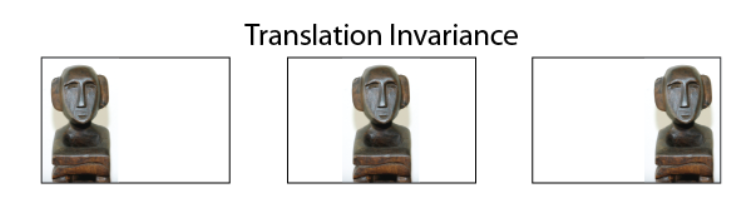
\includegraphics[width=0.8\textwidth]{img/translation_invariance.png}
    \caption{Las tres estatuas deben identificarse como iguales, aunque se ecuentren desplazadas.}
    \label{fig:invarianza_traslaciones}
\end{figure}

\medskip

\noindent Por otro lado, se conoce la \textbf{Invarianza frente a pequeñas deformaciones} (difeomorfismos) a la capacidad de reconocer la identidad de un objeto en una imagen a pesar de que este pueda haber sido alterado con pequeñas deformaciones.


\begin{figure}[!h]
  \centering
  
\includegraphics[width=0.5\textwidth]{img/Diffeomorphism.png}
  \caption{Acción de un difeomorfismo en una rejilla.}
  \label{fig:difeomorfismo}
\end{figure}

\begin{figure}[!h]
  \centering
  
\includegraphics[width=0.8\textwidth]{img/5_deformado.png}
  \caption{Todas las imágenes deberían clasificarse como 5, pese a las deformaciones.}
  \label{fig:deformaciones_5}
\end{figure}

\begin{figure}[!h]
  \centering
  
\includegraphics[width=0.5\textwidth]{img/1_excesivamente_deformado.png}
  \caption{Deformación excesiva que permite confundir el 1 con el 2 cuando se le aplica el difeomorfismo. Por eso nos centramos en \entrecomillado{pequeñas} deformaciones, para no alterar la identidad del objeto en la imagen.}
  \label{fig:deformaciones_1}
\end{figure}

\medskip


\noindent Esto motiva el estudio de las representaciones de traslaciones e invarianzas en las funciones de $L^2(\mathbb{R}^d)$, que son Lipschitz-continuas por la acción de difeomorfismos y que mantienen información de alta frecuencia para diferenciar entre distintos tipos de señales, con el objetivo de encontrar un operador que verifique todas estas propiedades y que presentaremos como la modelización matemática de una CNN.

\medskip

\noindent De esta manera, la invarianza por traslaciones, entendida en el contexto de las imágenes puede verse como trasladar cada pixel de la imagen en una misma dirección la misma distancia. En este sentido : 

\begin{definicion}
$L_cf(x)=f(x-c)$ es la traslación de $f \in L^2(\mathbb{R}^d)$ por $c \in \mathbb{R}^d$ .
\end{definicion}

\noindent Así, decimos que un operador $\Phi$ de  $L^2(\mathbb{R}^d)$ en un espacio de Hilbert $\mathcal{H}$ es invariante por traslaciones si $\Phi(L_cf(x))=\Phi(f)$ para todo $f \in L^2(\mathbb{R}^d)$ y para todo $c \in \mathbb{R}^d$. En el siguiente apartado trataremos el caso del módulo de la transformada de Fourier de $f$ como un ejemplo de un operador invariante por traslaciones. Sin embargo, es conocido el hecho de que aparecen inestabilidades frente a deformaciones en las altas frecuencias, y el mayor reto es preservar la Lipschitz-continuidad en esta situación.

\medskip

\noindent Para preservar la estabilidad en $L^2(\mathbb{R}^d)$ queremos que $\Phi$ sea no-expansiva. 

\begin{definicion}
Decimos que $\Phi$ es no-expansiva si: 
$$\forall (f,h) \in L^2(\mathbb{R}^d)^2 \; || \Phi(f)-\Phi(h)||_\mathcal{H} \leq ||f-h||$$
\end{definicion}

\noindent Por otro lado: 


\begin{definicion}
  Una función diferenciable $f: X \rightarrow \Omega$ dónde $X$ y $\Omega$ son variedades, es un \entrecomillado{Difeomorfismo} si $f$ es una biyección y su inversa $f^{-1}:\Omega \rightarrow X$ es también diferenciable. 
\end{definicion}


\noindent En nuestro caso, vamos a encargarnos de verificar la Lipschitz-continuidad relativa a la acción de pequeños difeomorfismos cercanos a las traslaciones. Dichos difeomorfismos transforman $x \in \mathbb{R}^d$ en $x-\tau (x)$ dónde $\tau$ es el campo de desplazamiento. 

\begin{definicion}
Denotemos $L_{\tau} f(x)=f(x-\tau(x))$ como la acción del difeomorfismo $\mathbb{1}-\tau$ en $f$.
\end{definicion} 

\medskip

\noindent Por otro lado, la condición de Lipschitz es la siguiente: 

\begin{definicion}
  Sea $f: M \rightarrow N$ una función entre dos espacios métricos $M$ y $N$ con sus respectivas distancias $d_M$ y $d_N$. Se dice que $f$ satisface la condición de Lipschitz si $\exists C>0$ tal que: 

  $$d_N(f(x),f(y))\leq C d_M(x,y), \; \; \forall x,y \in M$$
\end{definicion}

\noindent En nuestro caso, la $d_N$ que utilizaremos será la norma del espacio de Hilbert $\mathcal{H}$ de llegada, pero necesitamos definir de alguna manera una distancia $d_M$ entre los difeomorfismo $\mathbb{1}$ y $\mathbb{1}-\tau$ para escribir correctamente la condición de Lipschitz. Además, dado que el espacio de partida es $L^2(\mathbb{R}^d)$ y los puntos que vamos a comparar son las funciones $f$ y $L_\tau f=f(x-\tau(x))$ sabemos que $\|\Phi(f) - \Phi(L_cf) \|$ estará acotada por $\|f\| · d(\mathbb{1}, \mathbb{1}-\tau)$, de manera que necesitamos definir una distancia entre el difeomorfismo $\mathbb{1}$ y $\mathbb{1}-\tau$. Para ello, la topología débil \footnote{ recordemos que es la topología menos fina de un espacio normado que hace continuas todas las aplicaciones de su dual} en los difeomorfismos $C^2$  permite definir la siguiente aplicación, que utilizaremos como distancia:

\begin{definicion}
Así, se define una distancia entre $\mathbb{1}-\tau$ y $\mathbb{1}$ en cualquier subconjunto compacto $\Omega$ de $\mathbb{R}^d$ como 

\begin{equation} \label{eq::distancia}
  d_\Omega(\mathbb{1},\mathbb{1}-\tau) = \sup_{x \in \Omega} |\tau (x)| + \sup_{x \in \Omega} |\nabla \tau (x)| + \sup_{x \in \Omega}|H \tau (x)|
\end{equation}

\end{definicion}
\medskip

\noindent Dónde $|\tau (x)|$ es la norma euclídea en $\mathbb{R}^d$, $\nabla |\tau (x)|$ la norma del supremo de la matriz $\nabla \tau (x)$, y $|H \tau (x)|$ la norma del supremo del Hessiano.

\medskip

\noindent Así, podemos finalmente expresar la condición de Lipschitz que un operador debería satisfacer en nuestro caso:  

\medskip

\begin{definicion} \label{def::Lipschitz_cont}
\noindent Un operador invariante por traslaciones $\Phi$ se dice \entrecomillado{Lipchitz-continuo} por la acción de los difeomorfismos $C^2$  si para cualquier compacto $\Omega \subset \mathbb{R}^d$ existe una constante $C$ tal que para todo $f \in L^2(\mathbb{R}^d)$ con Soporte en $\Omega$ y para todo $\tau \in C^2(\mathbb{R}^d)$ se cumple:

\begin{equation} \label{eq::Lipschitz_condition}
  || \Phi(f)-\Phi(L_{\tau}f)||_\mathcal{H} \leq C||f||(\sup_{x \in \mathbb{R}^d} |\nabla \tau (x)| + \sup_{x \in \mathbb{R}^d}|H \tau (x)|)
\end{equation}
con  $|| \nabla \tau ||_\infty + ||H \tau ||_\infty < 1$ para asegurarnos de que la deformación sea invertible \cite{doi:10.1137/S0036141002404838}.
\end{definicion}

\medskip

\noindent Debido a que $\Phi$ es invariante a traslaciones, la cota superior de Lipschitz no depende de la amplitud máxima de traslación $\sup_{x \in \mathbb{R}^d}|\tau (x)|$ de la métrica del difeomorfismo \eqref{eq::distancia}. Por otro lado la continuidad Lipschitz de \eqref{eq::Lipschitz_condition} implica que $\Phi$ es invariante por traslaciones globales, pero es mucho más fuerte. $\Phi$ se ve poco afectada por los términos de primer y segundo grado de difeomorfismos que son traslaciones locales.

\medskip


\noindent Una vez presentadas las principales herramientas con las que trabajaremos, en las futuras secciones veremos como para la elección de ciertos operadores como el módulo de la transformada de Fourier existen problemas para satisfacer la condición de Lipschitz en altas frecuencias. Para solucionar el problema se optará por utilizar transformadas de ondeletas, pero esto abre nuevos problemas como serán el hecho de que no son invariantes por traslaciones. Por ello será necesario componer la transformada con un operador no lineal que será el módulo para obtener coeficientes invariantes por traslaciones. Este nuevo operador que consistirá en una cascada de convoluciones de operadores no lineales y no conmuntativos de manera que cada uno de ellos calcula el módulo de la transfomada de odeletas, y será este nuevo operador el que podremos interpretar como la modelización matemática de una CNN.

\subsection{Notación}

\begin{itemize}
    \item $|| \tau ||_\infty := \sup_{x \in \mathbb{R}^d} |\tau(x)|$
    \item $||\nabla \tau ||_\infty := \sup_{x \in \mathbb{R}^d} |\nabla \tau(x)|$
    \item $||\mathcal{H} \tau ||_\infty := \sup_{x \in \mathbb{R}^d} |\mathcal{H} \tau(x)|$ dónde $|\mathcal{H} \tau(x)|$ es la norma del tensor Hessiano. 
    \item La norma en $L^2(\mathbb{R}^d)$ de $f$ lo denotamos $||f||$.
    \item La norma de $f$ en $L^1(\mathbb{R}^d)$ lo denotamos $||f||_1=\int{|f(x)| dx}$.
    \item Se denota $g \circ f(x)=f(gx)$ a la acción de un elemento del grupo $g\in G$.
    \item Un operador  $\mathcal{R}$ parametrizado por $p$ es denotado por $\mathcal{R}[p]$ y $\mathcal{R}[\Omega]=\lbrace \mathcal{R}[p] \rbrace_{p \in \Omega}$. 
\end{itemize}

\section{Modelización Matemática de una Red Neuronal Convolucional} \label{ch:seccion12}

\noindent Nuestro primer objetivo será tratar de llegar a la modelización matemática de lo que es una \textbf{CNN}, para ello necesitamos en primer lugar definir un operador que denominaremos \textbf{propagador de dispersión} (PD) que será el que aplicaremos de forma recursiva en la cascada de convoluciones que modeliza una CNN, para ello explicaremos la problemática de elegir una operador \textit{lipschitz-continuo} bajo la acción de difeomorfismos e \textit{invariante por traslaciones}, para evitar problemas como las inestabilidades en altas frecuencias que se producen en las señales bajo la acción de difeomorfismos como ocurre si usamos la transformada de Fourier. 

\medskip

\noindent Tras esto  veremos posibles alternativas para evitar que se produzcan estas inestabilidades, mediante el uso de bases de la transformada de ondeletas de \textbf{Littlewood-Paley}. En concreto con esta segunda alternativa obtendremos un operador que es \textbf{Lipschitz-continuo} bajo la acción de difeomorfismos. 

\medskip

\noindent Después, nuestra tarea será conseguir calcular coeficientes que sean invariantes por traslaciones, y para ello necesitaremos utilizar un operador no lineal como es el módulo. 

\medskip

\noindent Una vez tengamos un operador con todas las propiedades anteriores presentaremos el \textbf{PD}, y será la aplicación en cadena de este operador anterior sobre un \entrecomillado{camino} de frecuencias y rotaciones el que definirá la modelización matemática de una Red Neuronal Convolucional.


\subsection{De Fourier a las ondeletas de Littlewood-Paley}

\subsubsection{El módulo de la Transformada de Fourier}

\noindent El análisis de Fourier tradicionalmente ha jugado un papel fundamental en el procesamiento de señales \cite{DigitalImageProcessing}, por lo que podría parecer un buen punto de partida para la construcción del \textbf{propagador de dispersión} emplear la \textbf{transformada de Fourier}, una de las herramientas matemáticas más potente en este campo. La intuición detrás de su fórmula es la de representar funciones no periódicas (pero que tienen área bajo la curva finita) como la integral de senos y cosenos multiplicados por una función que determina los pesos en cada instante. Formalmente tiene la siguiente expresión:

\begin{equation}
\widehat{f}(\omega):= \int{f(x)e^{-ix\omega}dx}=\int{f(x)\left[\cos{x\omega} -i\sin{x\omega}\right]dx}.
\end{equation}

\noindent Entre las propiedades más destacables de la transformada encontramos el hecho de que una función se puede recuperar sin pérdida de información a partir de su transformada de Fourier, lo cual nos permite poder trabajar en el \entrecomillado{Dominio de Fourier}\footnote{También llamado \entrecomillado{Dominio de Frecuencia}} ya que al calcular la integral, la función resultante sólo depende de $\omega$ (la frecuencia), y posteriormente pasar de nuevo al dominio original de la función, aplicando la inversa de la transformada sin pérdida de información.

\medskip

\noindent Esto a priori es algo atractivo, pues nos permitiría trabajar en un dominio más sencillo y extraer conclusiones que podemos traducir al dominio original de la señal sin pérdida de información. Además, en el estudio de señales se suele emplear el módulo de la transformada de Fourirer para evitar fases complejas en el análisis, de esta forma el operador que vamos a probar en primer lugar es: 

\begin{definicion}
$\Phi(f)=|\widehat{f}|$ módulo de la transformada de Fourier. 
\end{definicion}

\noindent Vamos a comprobar si se trata de un operador válido para nuestro propósito. Para ello necesitamos en primer lugar que sea un operador \textbf{Invariante por traslaciones}. Veamos  que sí cumple esta propiedad.

\begin{lema} \label{lema::invarianza_traslaciones}
    El operador $\Phi(f)=|\widehat{f}|$ es invariante por traslaciones.
\end{lema}

\begin{proof}
    \noindent Para ello tenemos que ver que si definimos para cada $c \in \mathbb{R}^d$, la traslación $L_cf(x)=f(x-c)$ se tiene que :  
    
    $$\widehat{L_cf}(w)=\int_{\mathbb{R}^d}{L_cf(x) e^{-ixw} dx}=\int_{\mathbb{R}^d}{f(x-c)e^{-ixw}dx}$$
    
    \noindent Y realizando el cambio de variable $x-c=y$ se tendría que: 
    
    \begin{align*}
        \int_{\mathbb{R}^d}{f(x-c)e^{-ixw}dx} &= \int_{\mathbb{R}^d}{f(y)e^{-i(y+c)w}dy}= \\      &=\int_{\mathbb{R}^d}{f(y)e^{-iyw}e^{-icw}dy}= \\ &=\int_{\mathbb{R}^d}=e^{-icw}\int_{\mathbb{R}^d}{f(y)e^{-iyw}dy}=e^{-icw}\widehat{f}(w)
    \end{align*}
    
    \noindent Por lo que se tiene que $|\widehat{L_cf}(w)|=|e^{-icw}| |\widehat{f}(w)|=|\widehat{f}(w)|$ y entonces $\Phi(f)=|\widehat{f}|$ es invariante a traslaciones. \qedhere
\end{proof}

\medskip
    
\noindent Sin embargo, la invaianza por traslaciones no es suficiente, necesitamos también que nuestro operador sea invariante frente a pequeñas deformaciones (difeomorfismos). De esta forma, un operador $\Phi(f)$ diremos que es estable frente a deformaciones si verifica \autoref{def::Lipschitz_cont}. Sin embargo, esta propiedad no la verifica el módulo de la Transformada de Fourier, como podemos ver a continuación:

\begin{lema} \label{lemma:TF_inestable_difeomorfismos}
El módulo de la Transformada de Fourier no es estable frente a pequeñas deformaciones y no es \entrecomillado{Lipschitz-continuo}.
\end{lema}

\begin{proof}
\noindent Vamos a considerar la función $\tau(x)\coloneqq \epsilon x$ con $0 < \epsilon << 1$. De esta forma $||\nabla \tau (x) ||_\infty = \epsilon$ y $||H\tau(x)||_\infty=0$ con esto, la condición de Lipschitz debería ser

$$\left|\left| \; |\widehat{f}| -|\widehat{L_\tau f}| \; \right|\right| \leq c ||f|| (||\nabla \tau ||_{\infty} + ||H\tau||_\infty) \leq c ||f|| \epsilon$$

\noindent Vamos a ver un contraejemplo con una función de una dimensión por simplicidad.

\medskip

\noindent Supongamos que tenemos $f(x)=e^{i \xi x} \Theta(x)=e^{i \xi x}e^{-|x|}$. Calculamos ahora $|\widehat{f}|$ y $|\widehat{L_\tau f}|$ teniendo en cuenta que :


\begin{align*}
  |\widehat{f}(\omega)|&=\left|  \int{f(x)e^{-ix\omega}dx}  \right | \\
  &=\left|  \int{f(x)e^{-ix\omega}dx}  \right | \\
  &=\left|  \int{e^{i \xi x}e^{-|x|}e^{-ix\omega}dx}  \right | \\
  &=\left|  \int{e^{-ix(\xi-\omega)}dx}  \right | \\
  &=\left|  \int{e^{-|x|}\left[\cos{x(\xi-\omega)} -i\sin{x(\xi-\omega)}\right]dx} \right| \\
\end{align*}

\noindent En el último paso podemos descomponer la integral en suma de dos, y para simplificar las operaciones llamamos $\beta=(\xi - \omega)$. Así, aplicando las siguientes fórmulas conocidas para el cálculo de integrales,


\begin{equation} \label{eq:res_auxiliar_1}
  \int_\mathbb{R} \cos(\beta x) e^{-|x|} dx= \frac{1}{1+\beta^2}
\end{equation}

\noindent y 

\begin{equation}\label{eq:res_auxiliar_2}
  \int_\mathbb{R} \sin(\beta x) e^{-|x|} dx= 0
\end{equation}

\noindent a nuestro caso concreto, obtenemos que: 

\begin{align*}
  |\widehat{f}(\omega)|&=\left|  \int{\cos{x\beta}e^{-|x|} dx} - i \int{\sin{x\beta}e^{-|x|} dx} \right| \\
  &=\frac{1}{1+\beta^2} \\
  &=\frac{1}{1+(\xi - \omega)^2}.
\end{align*} 

\noindent Ahora pasamos a calcular $|\widehat{L_\tau f}|$:

\begin{align*}
  |\widehat{L_\tau f}(\omega)| &= |\widehat{f}((1-\epsilon)\omega)| \\
  &=\left|  \int{f((1-\epsilon)x)e^{-ix\omega}dx}  \right | \\
  &=\left|  \int{e^{i \xi (1-\epsilon) x}e^{-|(1-\epsilon)x|}e^{-ix\omega}dx}  \right |. \\
\end{align*}

\noindent Ahora realizamos el siguiente cambio de variable

\begin{equation}
  \tilde{x}=(1-\epsilon) x \implies x=\frac{\tilde{x}}{1-\epsilon} 
\end{equation}

\begin{equation}
 d\tilde{x}=(1-\epsilon) dx \implies dx=\frac{1}{(1-\epsilon)}d\tilde{x}
\end{equation}

\noindent y aplicando los cambios a lo que teníamos nos queda

\begin{align*}
  |\widehat{L_\tau f}(\omega)| 
  &= \frac{1}{(1-\epsilon)}\left|  \int{f((1-\epsilon)x)e^{-ix\omega}dx}  \right | \\
  &=\frac{1}{(1-\epsilon)}\left|  \int{e^{i \xi \tilde{x}}e^{-|\tilde{x}|}e^{-i\frac{\tilde{x}}{(1-\epsilon)}\omega}d\tilde{x}}  \right | \\
  &=\frac{1}{(1-\epsilon)}\left|  \int{e^{i \left[ \frac{(1-\epsilon) \xi - \omega}{(1-\epsilon)}\right]\tilde{x}}e^{-|\tilde{x}|} d\tilde{x}}  \right | \\
  &=\frac{1}{(1-\epsilon)}\left|  \int{e^{i \tilde{\beta}\tilde{x}}e^{-|\tilde{x}|} d\tilde{x}}  \right |, \\
\end{align*}

\noindent como podemos ver, llegamos a una integral que se resuelve de la misma manera que en el caso anterior haciendo uso de \eqref{eq:res_auxiliar_1} y \eqref{eq:res_auxiliar_2}:

\begin{align*}
  |\widehat{L_\tau f}(\omega)| 
  &= \frac{1}{(1-\epsilon)} \frac{1}{1+\tilde{\beta}^2} \\
  &= \frac{1}{(1-\epsilon)} \frac{1}{1+\left[ \frac{(1-\epsilon) \xi - \omega}{(1-\epsilon)}\right]^2}. \\
\end{align*}


\noindent De esta forma hemos obtenido que para nuestro caso concreto de $f(x)=e^{i \xi x}e^{-|x|}$ ,


\begin{align*}
  \left\| |\widehat{L_\tau f}|-|\widehat{f}| \right\| &= \left\| \frac{1}{(1-\epsilon)} \frac{1}{1+\left[ \frac{(1-\epsilon) \xi - \omega}{(1-\epsilon)}\right]^2}-\frac{1}{1+(\xi - \omega)^2} \right\| \\
  &\geq  \left\| \frac{1}{1+\left[ \frac{(1-\epsilon) \xi - \omega}{(1-\epsilon)}\right]^2}-\frac{1}{1+(\xi - \omega)^2} \right\| \\
  &=\left(\int_{\mathbb{R}} \left| \frac{1}{1+\left[ \frac{(1-\epsilon) \xi - \omega}{(1-\epsilon)}\right]^2}-\frac{1}{1+(\xi - \omega)^2} \right|^2 d\omega\right)^{1/2}.
\end{align*}


\noindent A continuación vamos a intentar aproximar el valor del módulo de la integral, para ello en primer lugar vamos a realizar el siguiente cambio de variable 

\begin{align*}
  &t=\omega-\xi \implies \omega-(1-\epsilon)\xi= \omega-\xi + \epsilon\xi = t +\epsilon\xi \\
  &dt=d\omega.
\end{align*}

\noindent Así, obtenemos que: 

\begin{align*}
  \int_{\mathbb{R}} \left| \frac{1}{1+(\xi - \omega)^2} - \frac{1}{1+\left[ \frac{(1-\epsilon) \xi - \omega}{(1-\epsilon)}\right]^2} \right|^2 d\omega &\geq
  \left|\int_{\mathbb{R}} \left(  \frac{1}{1+(\xi - \omega)^2} - \frac{1}{1+\left[ \frac{(1-\epsilon) \xi - \omega}{(1-\epsilon)}\right]^2}  \right)^2 d\omega \right| \\
  &=\left|\int_{\mathbb{R}} \left(  \frac{1}{1+t^2} - \frac{1}{1+\left[ \frac{t+\epsilon\xi}{(1-\epsilon)}\right]^2}  \right)^2 d\omega \right| \\
\end{align*}

\noindent Representando la gráfica $g_1(t)= \frac{1}{1+t^2}$, podemos ver cómo el valor de su integral se acumula en torno al origen de coordenadas, y en cambio $g_2(t)=\frac{1}{1+\left[ \frac{t+\epsilon\xi}{(1-\epsilon)}\right]^2}$ e una traslación y escalado de la función anterior. De esta forma, si $\epsilon\xi$ es muy grande, el área de la función $g_2(t)$ será prácticamente cero en la región del espacio dónde $g_1(t)$ concentra su integral. Dicho de otra forma, las dos funciones tendrían soporte disjunto.

\noindent De esta forma, podemos tomar una constante $M>0$ tal que para un valor de $\xi$ elevado se cumpla que: 

\begin{align*}
  \int_{\mathbb{R}} \left| \frac{1}{1+(\xi - \omega)^2} - \frac{1}{1+\left[ \frac{(1-\epsilon) \xi - \omega}{(1-\epsilon)}\right]^2} \right|^2 d\omega 
  &\geq \int_{-M}^{M} (g_1(t)-g_2(t))^2 dt \\
  &\approx \int_{-M}^{M} g_1(t)^2 dt. \\
\end{align*}

\noindent Y como $\xi$ puede ser arbitrariamente grande, intuitivamente el intervalo en el que ambas funciones tienen soporte disjunto crece de forma indefinida lo cual nos permite realizar la siguiente aproximación teniendo en cuenta que $g_1(t)=\widehat{f}$:

\begin{equation} \label{eq::1.1}
  \left\| |\widehat{f}| -|\widehat{L_\tau f}| \; \right\| \sim \|g_1(t) \|=\|f\|. 
\end{equation}

\noindent Dónde la última igualdad la hemos realizado gracias a la fórmula de Plancharel que en el caso de $\mathbb{R}^d$ es: 

\begin{equation} \label{eq::Plancharel}
  \int_{\mathbb{R}^d} \left|f(x)\right|^2 dx= \int_{\mathbb{R}^d}\left|\widehat{f}(\omega)\right|^2 d\omega.
\end{equation}

\noindent Luego hemos demostrado que en este caso particular el operador $|\widehat{f}|$ no cumple la condición de Lipschitz, pues como hemos mencionado antes, $\xi$ puede ser arbitrariamente grande y de esta forma, que la diferencia anterior pueda ser todo lo grande que se quiera.

\begin{figure}[!h]
  \centering
  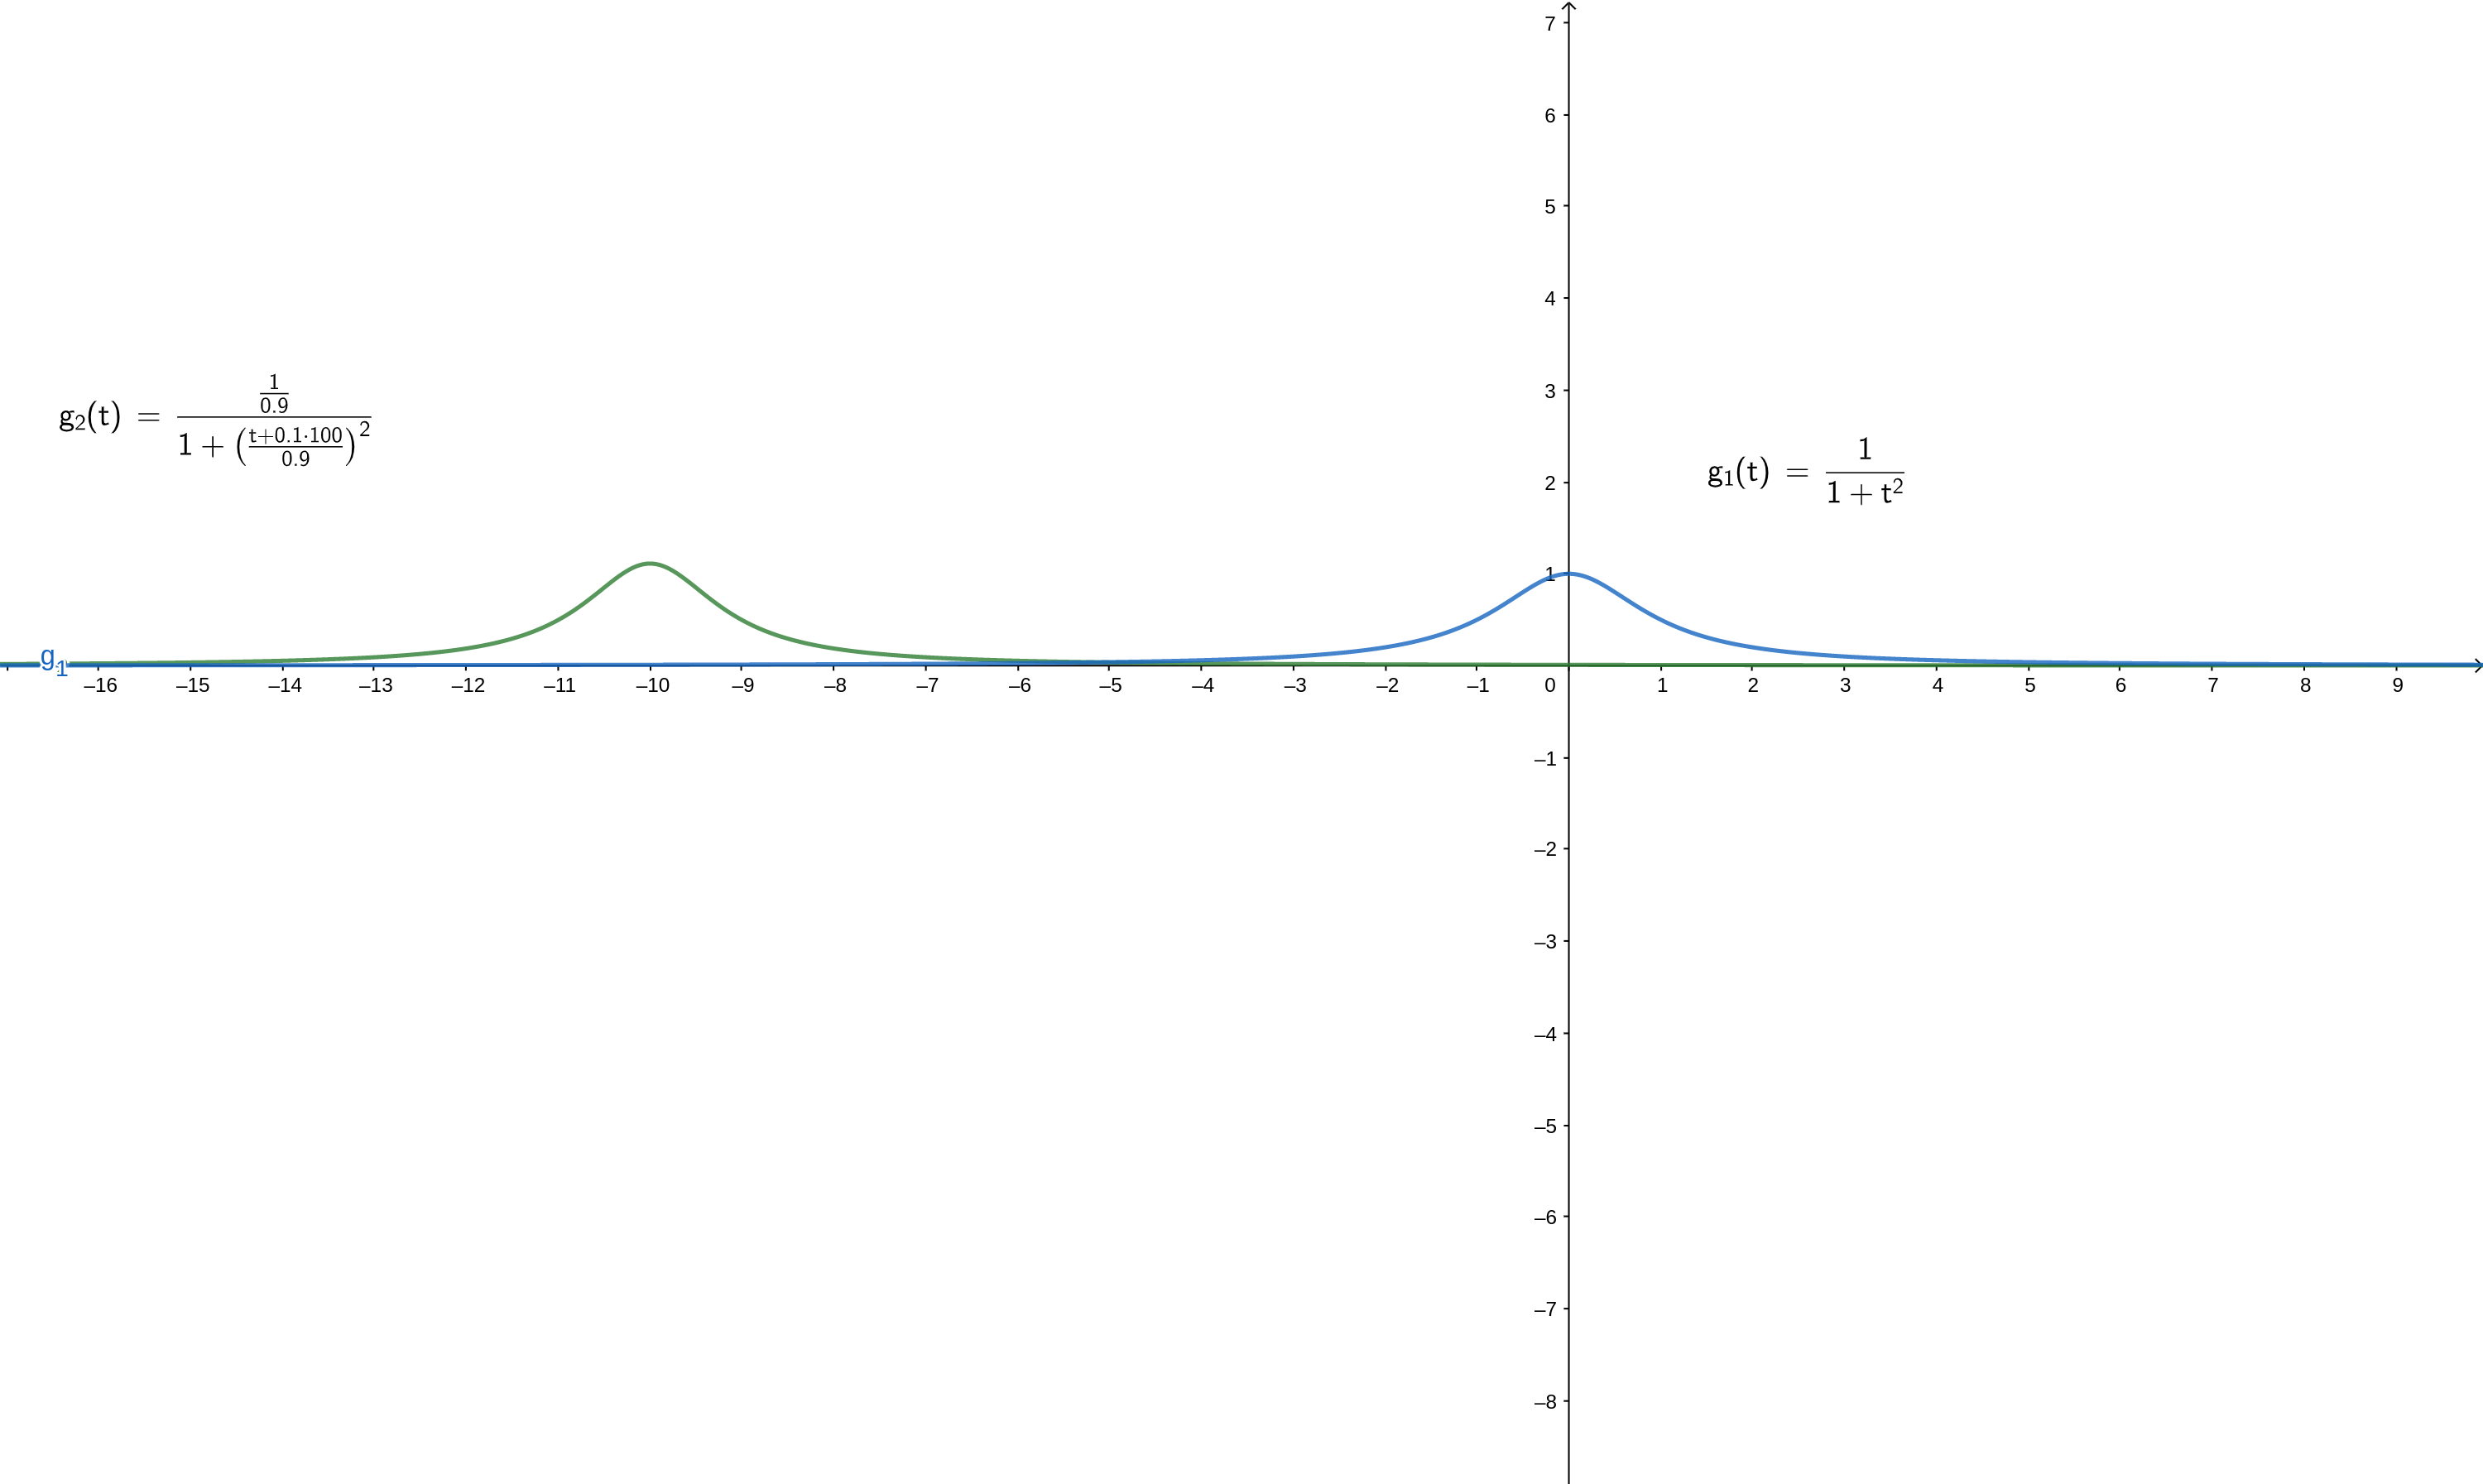
\includegraphics[width=1.0\textwidth]{img/geogebra-export_contraejemplo_Fourier.png}
  \caption{Como podemos ver en la imagen, para los valores $\epsilon=0.1$, $\xi=100$ y $M=5$ ambas funciones tienen soporte casi disjunto de manera que la diferencia entre ellas en el intervalo $[-5,5]$ coincide prácticamente con la integral de $g_1(t)$.}
  \label{fig:Grafica_funciones}
\end{figure}

\end{proof}
    
\medskip

\noindent Por esto, lo que haremos será reemplazar las ondas sinusoidales de la transformada de Fourier por funciones localizadas con un soporte mayor en altas frecuencias que nos permitan evitar estas complicaciones, que tendrán un mejor rendimiento en nuestro propósito. Estas funciones se denominan \textbf{ondeletas}. 

\medskip

\subsubsection{Alternativa: Las ondeletas}

\noindent Las ondeletas \cite{MallatWavelets} son pequeñas ondas estables bajo la acción de deformaciones, al contrario que las ondas sinusoidales de Fourier. Definiremos la transformada de ondeletas y veremos que calcula, mediante convoluciones con bases de ondeletas, coeficientes estables bajo la acción de difeomorfismos.

\medskip

\noindent Al contrario que las bases de Fourier, las bases de ondeletas definen  representaciones dispersas de señales regulares a trozos, que podrían incluir transiciones y singularidades. En las imágenes, los mayores coeficientes de las ondeletas se localizan en el entorno de las esquinas y en las texturas irregulares.

\medskip

\noindent A modo de ejemplo vamos a ver la base de Haar que, aunque no sea la que utilicemos para construir nuestro propagador de dispersión, puede ayudar a entender mejor la filosofía de las ondeletas. Se construye a partir de la siguiente función: 

$$ \psi(t)= \begin{cases} 
      1 & 0\leq t < 1/2 \\
      -1 & 1/2\leq t < 1 \\
      0 & \; en \; otro \; caso
   \end{cases}$$

\begin{figure}[!h]
  \centering
  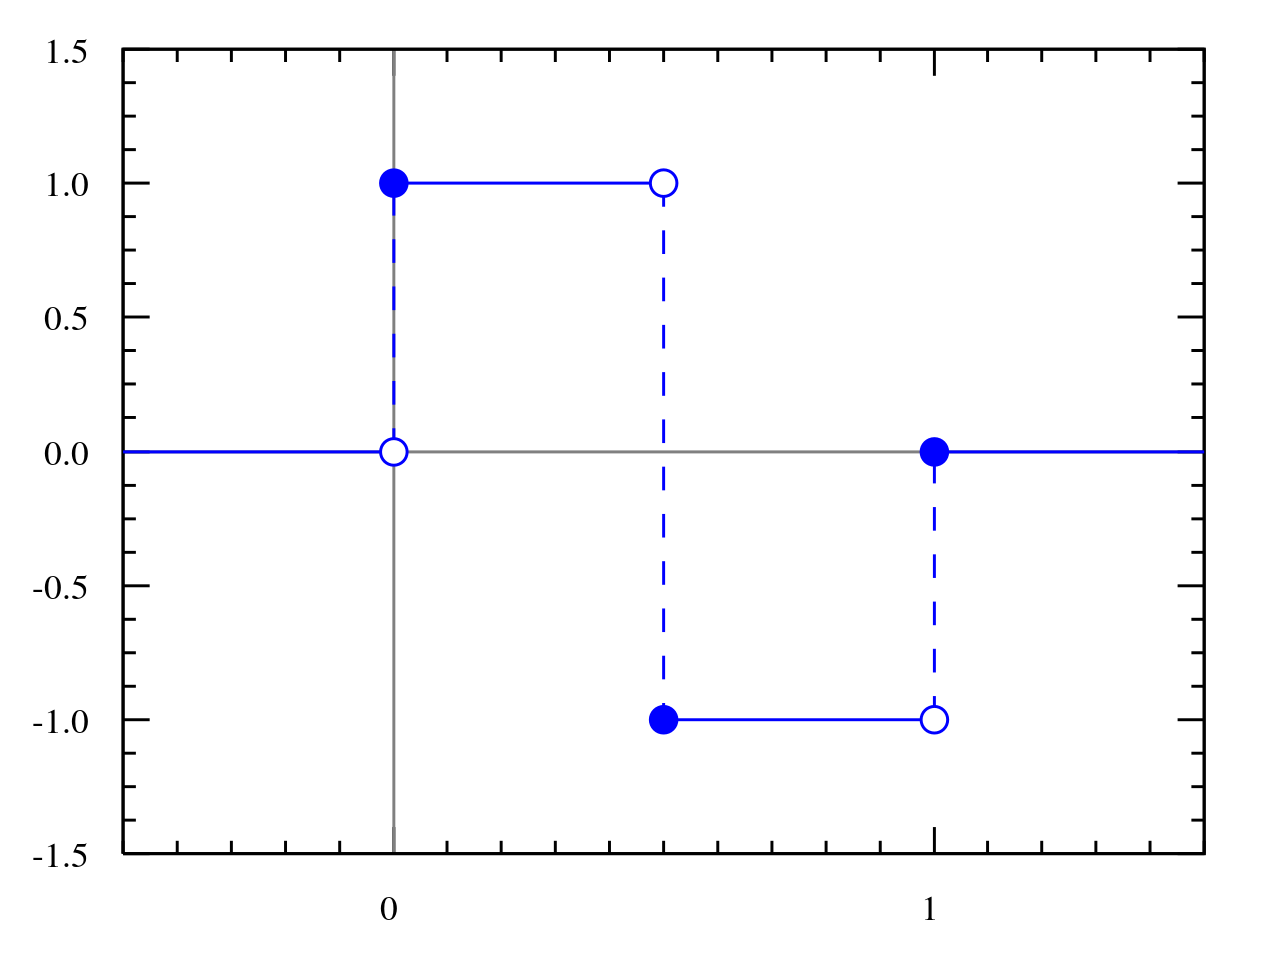
\includegraphics[width=0.5\textwidth]{img/Haar_wavelet.png}
  \caption{Representación gráfica de la ondeleta de Haar.}
  \label{fig:Ondeleta_de_Haar}
\end{figure}

\noindent A esta ondeleta la denominamos \textbf{ondeleta Madre}, pues a partir de ella, podemos generar la siguiente base ortonormal

\medskip

$$\left \lbrace \psi_{j,n}(t)= \frac{1}{\sqrt{2^j}} \psi\left(\frac{t-2^jn}{2^j}\right) \right\rbrace_{(j,n) \in \mathbb{Z}^2}$$

\noindent del espacio $L^2(\mathbb{R})$ de señales con energía finita. Si recordamos, en este espacio la norma se define como 

  $$||f||^2=\int_{-\infty}^{+\infty} |f(t)|^2 dt < +\infty.$$

\noindent Así, cualquier señal $f$ de energía finita puede ser representada por los coeficientes que se obtienen mediante el producto interno en $L^2(\mathbb{R})$ con la base anterior: 

$$\langle f,\psi_{j,n} \rangle =\int_{-\infty}^{+\infty} f(t) \psi_{j,n} (t) dt  $$

\noindent y puede recuperarse sumando en su base ortonormal:

$$f=\sum_{j=-\infty}^{+\infty}\sum_{n=-\infty}^{+\infty}  \langle f,\psi_{j,n} \rangle \psi_{j,n} $$

\noindent Esto nos permite (igual que pasaba con el módulo de la Transformada de Fourier) trabajar en un dominio más sencillo que nos permite procesar la información con mayor rapidez y posteriormente reconstruir la señal a partir de los coeficientes sin perder información. Algunas propiedades serían: 

\newpage

\begin{itemize}
  \item Cada ondeleta $\psi_{j,n}$ tiene media $0$ en su soporte $[2^jn, 2^j(n+1)]$.
  \item Si $f$ es localmente regular y $2^j$ es pequeño, entonces es casi constante en su intervalo y su coeficiente de ondeleta $\langle f,\psi_{j,n} \rangle$ es prácticamente cero.
  \item los mayores coeficientes se localizan en los cambios bruscos de intensidad de señal, como pueden ser los bordes, las esquinas o las texturas en las imágenes.
\end{itemize}

\noindent Para el caso concreto de imágenes \footnote{ver por ejemplo sección 1.1 de \cite{MallatWavelets}}, las bases de ondeletas ortonormales pueden construirse a partir de bases ortonormales en señales de una dimensión. Así, a partir de tres ondeletas $\psi^1(x)$, $\psi^2(x)$ y$\psi^3(x)$ con $x=(x_1,x_2)\in \mathbb{R}^2$, dilatadas por el factor $2^j$ y trasladadas por $2^jn$ con $n=(n1,n2)\in \mathbb{Z}^2$, se construye una base ortonormal para el espacio $L^2(\mathbb{R}^2)$: 
$$\left \lbrace \psi_{j,n}^k(x)= \frac{1}{\sqrt{2^j}} \psi^k\left(\frac{x-2^jn}{2^j}\right) \right \rbrace_{(j,n) \in \mathbb{Z}^2}$$

\medskip

\noindent El soporte de la ondeleta $\psi_{j,n}^k(x)$ es un cuadrado proporcional a la escala $2^j$. Las bases de ondeletas en dos dimensiones se discretizan para definir bases ortonormales de imágenes de N píxeles.


\noindent Del mismo modo que en una dimensión, los coeficientes de ondeletas $\langle f,\psi_{j,n}^k \rangle$ serán pequeños si $f(x)$ es regular, y serán grandes cerca de los cambios bruscos de frecuencias como en los bordes o esquinas de las imágenes, como podemos ver en \autoref{fig:ejemplo_haar}. Los filtros resaltan los bordes en tres direcciones, horizontal (derecha) vertical (abajo) y en diagonal (abajo derecha).

\begin{figure} [!h]
  \centering
  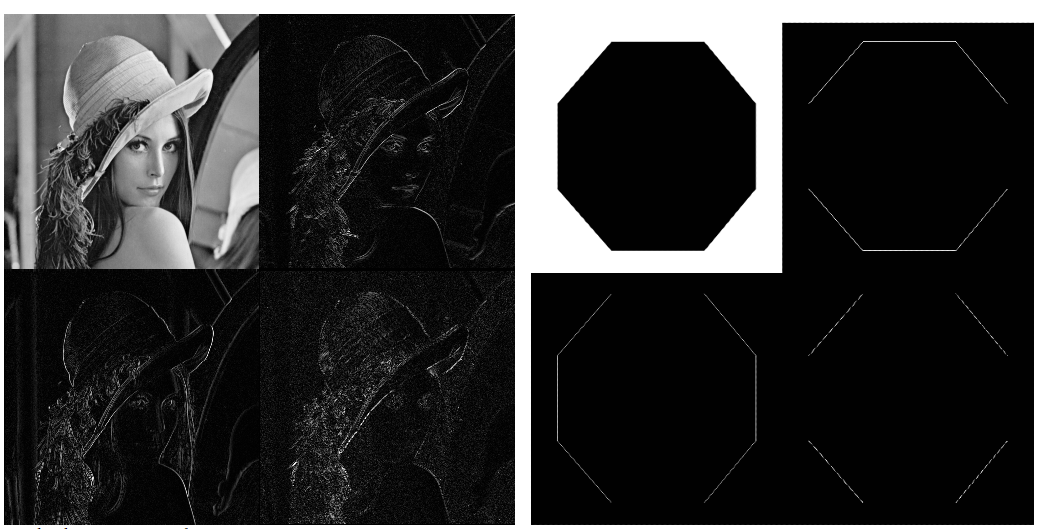
\includegraphics[width=0.8\textwidth]{img/ejemplos_haar_basis.png}
  \caption{Ejemplos de aplicar la base de Haar a dos imágenes \cite{HaarBasis}.}
  \label{fig:ejemplo_haar}
\end{figure}

\medskip 

\noindent Volviendo al propósito de definir el propagador de dispersión, la ondeleta madre que elijamos y la base ortogonal que forme se verán afectadas normalmente por escalados y rotaciones, por lo tanto definimos: 

\begin{definicion}
  Una ondeleta madre escalada por un factor $2^{-j}$ con $j \in \mathbb{Z}$ y rotada por $r \in G$ siendo $G$ el grupo finito de rotaciones, se escribe: 

  $$\psi_{2^j r}(x)=2^{dj} \psi(2^j r^{-1} x).$$
\end{definicion}


\medskip

\noindent Su transformada de Fourier es $\widehat{\psi_{2^j r}}(\omega)=\widehat{\psi}(2^j r^{-1} \omega)$.

\medskip

\noindent La transformada de dispersión que usaremos tendra una base de ondeletas generada por una ondeleta madre del tipo:

$$\psi(x)=e^{i\eta x} \Theta(x)$$

\noindent Donde $\widehat{\Theta}(x)$ es una función real centrada en una bola de baja frecuencia en $x=0$, cuyo radio es del orden de $\pi$.

\medskip

\noindent Y como podemos ver:

\begin{equation}
  \widehat{\psi}(\omega)=\int_{\mathbb{R}^d}e^{i \eta x} \Theta(x) e^{-i\omega x} dx=\int_{\mathbb{R}^d}\Theta(x) e^{ix(\omega-\eta)} dx=\widehat{\Theta}(\omega-\eta).
\end{equation}

\medskip

\noindent Por lo tanto, $\widehat{\psi}(\omega)$ es real y centrada en una bola de mismo radio pero centrada en $\omega=\eta$ que tras el escalado y rotación: 
$$\widehat{\psi}_\lambda(\omega)= \widehat{\Theta} (\lambda^{-1}\omega-\eta),$$ 

\noindent donde $\lambda=2^jr \in 2^{\mathbb{Z}}\times G$. 

\noindent Por lo tanto $\widehat{\psi}_\lambda(\omega)$ recubre una bola centrada en $\lambda^{-1}\eta$ con radio proporcional a $|\lambda|=2^j$.
 
\medskip 

\subsubsection{La Transformada de Littlewood-Paley}

\noindent Una vez conocemos un poco más en profundidad las ondeletas y su funcionamiento, pasamos a presentar la \textbf{Transformada de ondeleta de Littlewood-Paley}, que es la que emplearemos para construir el propagador de dispersión.

\medskip

\noindent Se trata de una representacion redundante que calcula convoluciones para todo $x \in \mathbb{R}^d$ sin realizar sub-muestreo: 

\begin{equation}
  \forall x \in  \mathbb{R}^d \;\; W[\lambda]f(x)= f \ast \psi_\lambda(x)=\int f(u)\psi_\lambda(x-u) du .
\end{equation}

\noindent Dónde $\ast$ denota la operación de convolución. 

\medskip

\noindent Calculamos su transformada de Furier, para ello tendremos en cuenta el teorema de Convolución de la Transformada de Fourier, el cual dice: 

\begin{teorema} \label{Teorema::Convolucion}
 Sean $f$ y $g$ dos funciones integrables.

 Si 

 $$h(x)=(f\ast g)(x)=\int f(y)g(x-y) dy$$

 Entonces: 

 $$\widehat{h}(\omega)=\widehat{f}(\omega) \widehat{g}(\omega)$$

 y 

 $$h(x)=(f \ast g)(x)= \int \widehat{f}(\omega) \widehat{g}(\omega) e^{-i\Omega x} d\omega$$
 
\end{teorema}

De esta manera, se tiene que: 

$$\widehat{W[\lambda]f(\omega)}=\widehat{f}(\omega)\widehat{\psi_\lambda}(\omega)=\widehat{f}(\omega)\widehat{\psi}(\lambda^{-1}\omega).$$

\noindent Además, teniendo en cuenta la propiedad que nos dice que si la función $f$ es real, entonces su transformada coincide con el conjugado complejo $\widehat{f}(-\omega)=\overline{\widehat{f}(\omega)}$ podemos ver que: 

\begin{itemize}
  \item si $\widehat{\psi}(\omega)$ y $f$ son reales entonces $W[-\lambda]f= \overline{W[\lambda]f}$, utilizando la misma propiedad de antes. Además, si denotamos por $G^{+}$ al cociente de G con $\lbrace-\mathbb{1},\mathbb{1}\rbrace$, conjunto en el cual las dos rotaciones $r$ y $-r$ son equivalentes, sería suficiente calcular $W[2^jr]f$ para las rotaciones "positivas" de $G^{+}$.
  \item En cambio, si $f$ fuese compleja, entonces $W[2^jr]f$ tendría que calcularse para todo $r \in G$.
\end{itemize}

\medskip
 
\noindent La transformada de Littlewood-Paley a una cierta escala $2^J$ sólo mantiene las ondeletas de frecuencias $2^j>2^{-J}$ pues el resto de ondeletas de la base no tendrían soporte. De esta forma, las bajas frecuencias que no son cubiertas por estas ondeletas vienen dadas por un promedio en el dominio proporcional a $2^J$:

\begin{equation}
  A_Jf=f \ast \phi_ {2^J} \; \; con \; \phi_ {2^J}(x)=2^{-dJ} \phi(2^{-J}x).
\end{equation}

\medskip

\noindent Así, si $f$ fuese real, entonces la transformada de ondeleta tendría la siguiente expresión: 

$$W_J f=\lbrace A_Jf,(W[\lambda]f)_{\lambda \in \Lambda_J} \rbrace$$ 

\noindent Es decir, estaría formada por el promedio de todas las odeletas de la base que no tienen soporte a la escala fijada $2^J$, y el conjunto de coeficientes producidos al convolucionar cada elemento de la base con $2^j>2^{-J}$ con la señal $f$. Para denotar esto indexamos por $\Lambda_J=\lbrace \lambda=2^jr:\;r\in G^{+}, \; 2^j>2^{-J}\rbrace$. 

\medskip

\noindent Su norma sería: 

\begin{equation}
  ||W_Jf||^2=||A_Jf||^2+\sum_{\lambda \in \Lambda_j} ||W[\lambda]f||^2.
\end{equation}

\medskip
 
\noindent Si $J=\infty$ entonces todas las ondeletas de la base obtendrían coeficientes no nulos y por lo tanto 
$$W_\infty f=\lbrace W[\lambda]f\rbrace_{\lambda \in \Lambda_\infty},$$ 

\noindent con $\Lambda_\infty=2^\mathbb{Z} \times G^{+}$. 

\noindent Su norma en este caso sería 

$$||W_\infty f||^2=\sum_{\lambda \in \Lambda_\infty} ||W[\lambda]f||^2.$$

\noindent En el caso en que $f$ sea compleja, se incluyen todas las rotaciones $W_Jf=\lbrace A_J f,(W[\lambda]f)_{-\lambda,\lambda \in \Lambda_J} \rbrace$ y $W_\infty f=\lbrace W[\lambda]f\rbrace_{-\lambda,\lambda \in \Lambda_\infty}$. 

\medskip

\noindent La siguiente proposición da una condición estándar de Littlewood-Paley para que $W_J$ sea unitario.

\begin{proposicion} \label{unitario}
 Para cualquier $J \in \mathbb{Z}$ o $J=\infty$, $W_J$ es unitario en el espacio de funciones reales o complejas de $L^2(\mathbb{R}^d)$ si y sólo si para casi todo $\omega \in \mathbb{R}^d$: 
    \begin{equation}\label{eq::1.2}
        \beta \sum_{j=-\infty}^\infty \sum_{r \in G} |\widehat{\psi}(2^{-j}r^{-1}\omega)|^2=1 \; \; y
        \;\;|\widehat{\phi}(\omega)|^2= \beta \sum_{j=-\infty}^0 \sum_{r\in G} |\widehat{\psi}(2^{-j}r^{-1}\omega)|^2,
    \end{equation}
 Dónde $\beta=1$ para funciones complejas y $\beta=\frac{1}{2}$ para funciones reales.
\end{proposicion}

\begin{proof}
\noindent Si $f$ es una función compleja, $\beta=1$, y vamos a demostrar que \eqref{eq::1.2} es equivalente a : 

\begin{equation} \label{eq::1.3}
  \forall J \in \mathbb{Z} \; \; \; \left|\widehat{\phi}\left(2^J\omega\right)\right|^2 + \sum_{j>-J,r\in G}\left|\widehat{\psi}\left(2^{-j}r^{-1}\omega\right)\right|^2=1.
\end{equation}

\noindent Para ello partimos de que si $\beta=1$ se tiene sustituyendo en \eqref{eq::1.2} que: 
     \begin{align*}
        \sum_{j=-\infty}^\infty \sum_{r \in G} |\widehat{\psi}(2^{-j}r^{-1}\omega)|^2=1 & \; \; y
        \;\;|\widehat{\phi}(\omega)|^2= \sum_{j=-\infty}^0 \sum_{r\in G} |\widehat{\psi}(2^{-j}r^{-1}\omega)|^2.
    \end{align*}

\noindent Si ahora sumamos $\sum_{j=0}^{\infty} \sum_{r\in G} |\widehat{\psi}(2^{-j}r^{-1}\omega)|^2$ en el segundo término obtenemos: 

$$|\widehat{\phi}(\omega)|^2 + \sum_{j=0}^{\infty} \sum_{r\in G} |\widehat{\psi}(2^{-j}r^{-1}\omega)|^2=1.$$

\noindent Por otro lado si vamos a la expresión a la que queremos llegar se tiene que: 

$$\forall J \in \mathbb{Z} \; \; \; \left|\widehat{\phi}\left(2^J\omega\right)\right|^2 + \sum_{j>-J,r\in G}\left|\widehat{\psi}\left(2^{-j}r^{-1}\omega\right)\right|^2=1 \iff \forall J \in \mathbb{Z} \; \; \; \left|\widehat{\phi}\left(2^J\omega\right)\right|^2=\sum_{j=-\infty}^{-J} \sum_{r\in G} |\widehat{\psi}(2^{-j}r^{-1}\omega)|^2.$$

\noindent Con lo que si demostramos esto último tendríamos que \eqref{eq::1.2} y \eqref{eq::1.3} son equivalentes para el caso $\beta=1$. 


     \begin{align*}
        \left|\widehat{\phi}\left(2^J\omega\right)\right|^2 & =\sum_{j=-\infty}^{0} \sum_{r\in G} |\widehat{\psi}(2^{-j}r^{-1}2^J\omega)|^2 \\
        & = \sum_{j=-\infty}^{0} \sum_{r\in G} |\widehat{\psi}(2^{J-j}r^{-1}\omega)|^2  \\
        & =\sum_{j=-\infty}^{-J} \sum_{r\in G} |\widehat{\psi}(2^{-j}r^{-1}\omega)|^2  
    \end{align*}
    
\noindent con lo que queda demostrado que \eqref{eq::1.2} y \eqref{eq::1.3} son equivalentes. Teniendo en cuenta que $\widehat{W\left[2^jr\right]f}(\omega)=\widehat{f}(\omega)\widehat{\psi}_{s^jr}(\omega)$, multiplicando \eqref{eq::1.3} por $|\widehat{f}(\omega)|^2$ obtenemos: 

$$\forall J \in \mathbb{Z} \; \; \; \left|\widehat{\phi}\left(2^J\omega\right)\right|^2 \left|\widehat{f}(\omega)\right|^2 + \sum_{j>-J,r\in G}\left|\widehat{f}(\omega)\right|^2\left|\widehat{\psi}\left(2^{-j}r^{-1}\omega\right)\right|^2=\left|\widehat{f}(\omega)\right|^2.$$

\noindent Si ahora integramos en ambos miembros en $\mathbb{R}^d$ obtenemos: 

     \begin{align*}
        \int_{\mathbb{R}^d}\left(\left|\widehat{\phi}\left(2^J\omega\right)\right|^2 \left|\widehat{f}(\omega)\right|^2 + \sum_{j>-J,r\in G}\left|\widehat{f}(\omega)\right|^2\left|\widehat{\psi}\left(2^{-j}r^{-1}\omega\right)\right|^2 \right) d\omega=\int_{\mathbb{R}^d}\left|\widehat{f}(\omega)\right|^2 d\omega.
    \end{align*}

\noindent Si la aplicamos \eqref{eq::Plancharel} se obtiene:

$$\int_{\mathbb{R}^d}\left(\left|\phi\left(2^J\omega\right)\right|^2 \left|f(\omega)\right|^2 + \sum_{j>-J,r\in G}\left|f(\omega)\right|^2\left|\psi\left(2^{-j}r^{-1}\omega\right)\right|^2 \right) d\omega=\int_{\mathbb{R}^d}\left|f(\omega)\right|^2 d\omega.$$

\noindent Si ahora recordamos la expresión (2.6), tenemos que la expresión anterior equivale a:

$$||A_Jf||^2+\sum_{\lambda \in \Lambda_j} ||W[\lambda]f||^2=||W_J f||^2=||f||^2,$$

\noindent que es válido para todo $J$ y en particular también cuando $J=\infty$.

\medskip

\noindent Recíprocamente, si tenemos que $||W_J f||^2=||f||^2$ entonces \eqref{eq::1.3} se verifica para casi todo $\omega$. De no ser así podríamos contruir una función $f$ no nula cuya transformada de fourier $\widehat{f}$ tuviera soporte en el dominio de $\omega$ dónde \eqref{eq::1.3} no fuera válido, y en estos casos al aplicar la fórmula de Plancherel se verificaría que $||W_J f||^2 \neq ||f||^2$ contradiciendo la hipótesis. Y como la expresión \eqref{eq::1.3} era equivalente a la que nos daba el teorema tenemos demostrado el resultado para el caso en que $f$ sea compleja. 

\medskip

\noindent Si ahora $f$ es real entonces $|\widehat{f}(\omega)|=|\widehat{f}(-\omega)|$ lo que implica que $||W[2^jr]f||=||W[-2^jr]f||$. Por lo que $||W_J f||$ permanece constante si restringimos $r$ a $G^+$ y multiplicando $\psi$ por $\sqrt{2}$ se obtiene la condición \eqref{eq::1.2} con $\beta=\frac{1}{2}$. \qedhere

\end{proof}

\medskip


\subsubsection{Convenios para futuras secciones}

\noindent Llegados a este punto, ya tenemos la transformada de ondeletas que vamos a utilizar para la construcción del PD, ahora vamos a establecer algunas características que impondremos a los distintos elementos que la componen y que usaremos de ahora en adelante: 

\begin{itemize}
    \item $\widehat{\psi}$ es una función real que satisface la condición \eqref{eq::1.2}. Lo que implica que $\widehat{\psi}(0)=\int \psi(x)dx=0$ y $|\widehat{\phi}(r\omega)|=|\widehat{\phi}(\omega)| \;\; \forall r\in G$.
    \item $\widehat{\phi}(\omega)$ es real y simétrica, por lo que $\phi$ también lo será y $\phi(rx)=\phi(x) \;\; \forall r \in G$. 
    \item Suponemos que $\phi$ y $\psi$ son dos veces diferenciables y su decrecimineto así como el de sus derivadas de primer y segundo orden es $O((1+|x|)^{-d-2})$.
\end{itemize}

\medskip

\noindent Un cambio de variable en la integral de la transformada de ondeleta nos muestra que si $f$ se escala y rota, $2^lg \circ f=f(2^lgx)$ con $2^lg \in 2^{\mathbb{Z}} \times G$, entonces la transformada de ondeleta se escala y rota de acuerdo a: 

\begin{equation}
  W[\lambda](2^lg\circ f)=2^lg \circ W[2^{-l}g\lambda]f.
\end{equation}

\medskip

\noindent Como $\phi$ es invariante a traslaciones en $G$, podemos comprobar que $A_J$ conmuta con las rotaciones de $G$: $A_J(g\circ f)=g\circ A_J f \;\; \forall g \in G$. 

\subsection{El operador de dispersión sobre un camino ordenado}

%Esto debería intentar explicarlo mejor?
\noindent La transformada de Littlewood-Paley definida anteriormente es Lipschitz-conitnua bajo la acción de difeomorfismos, porque las ondeletas son funciones regulares y localizadas. Sin embargo, todavía no es invariante a traslaciones y $W[\lambda]f=f\ast\psi_\lambda$ se traslada cuando lo hace $f$. Así, nuestro próximo objetivo será conseguir calcular coeficientes que sean invariantes a traslaciones, que permanezcan estables bajo la acción de difeomorfismos y que retengan la información en altas frecuencias que proporcionan las ondeletas, reuniendo todas estas características tendríamos el operador que necesitamos para la construcción del PD. 

\medskip 

\noindent Los coeficientes invariantes por traslaciones los obtendremos gracias a la acción de un operador no lineal aplicando el siguiente lema: 

%No se si perder tiempo en buscar la dem
\begin{lema} \label{lema:Invarianza_traslaciones_integral}
  Si $U[\lambda]$ es un operador definido en $L^2(\mathbb{R}^d)$, no necesariamente lineal pero que conmuta con traslaciones, entonces $\int_{\mathbb{R}^d} U[\lambda]f(x)dx$ es invariante a traslaciones si es finito.
\end{lema}

\begin{proof}
  Sea $f \in L^2(\mathbb{R}^d)$, $c \in \mathbb{R}^d$ y $L_cf(x)=f(x-c)$ una traslación de $f$, como $U[\lambda]f$ conmuta con traslaciones se tiene que: 
  \begin{align*}
    U[\lambda]L_cf(x)&=U(f(x-c)) \\
    &=U(f)(x-c) \\
    &=L_cU[\lambda]f(x)\\
  \end{align*}

  \noindent Vamos a comprobar ahora que si $\int_{\mathbb{R}^d} U[\lambda]f(x)dx$ es finito, entonces la integral es invariante a traslaciones. En otras palabras, queremos comprobar que : 

  $$\int_{\mathbb{R}^d} U[\lambda]L_cf(x)dx=\int_{\mathbb{R}^d} U[\lambda]f(x)dx$$

  Para ello, si tenemos en cuenta la conmutatividad del operador $U[\lambda]$ se tiene que 
  
  \begin{align*}
    \int_{\mathbb{R}^d} U[\lambda]L_cf(x)dx &= \int_{\mathbb{R}^d} U[\lambda](f(x-c))dx \\
    &= \int_{\mathbb{R}^d} U[\lambda](f)(x-c)dx. \\
  \end{align*}

  \noindent Y tras esto basta tener en cuenta el cambio de variable $y=x-c$ que tiene Jacobiano $J=1$ y se tendría que en la expresión anterior
  \begin{align*}
    \int_{\mathbb{R}^d} U[\lambda](f)(x-c)dx = \int_{\mathbb{R}^d} U[\lambda](f)(y)dy .\\
  \end{align*}
  
  \noindent Por lo que la integral es invariante por traslaciones.
\end{proof}

\noindent En nuestro caso $W[\lambda]f=f\ast\psi_\lambda$ es un ejemplo trivial de este lema, pues se trata de un operador que conmuta con traslaciones y $\int_{\mathbb{R}^d} f \ast \psi(x) dx=0$ porque $\int_{\mathbb{R}^d} \psi(x)dx=0$.

\medskip

\noindent Esto nos enseña, que para obtener un operador invariante por traslaciones y no trivial $U[\lambda]f$, es necesario componer $W[\lambda]$ con un operador extra $M[\lambda]$ que sea \entrecomillado{no lineal}, y que se conoce como "demodulación", que transforma $W[\lambda]f$ en una función de menor frecuencia con integral distinta de cero. Además, la elección de $M[\lambda]$ debe preservar la Lipschitz-continuidad bajo la acción de difeomorfismos.    
En resumen, queremos un operador no lineal que produzca coeficientes invariantes por traslaciones no triviales y que además conserve la Lipschitz-continuidad.


\medskip

\noindent Vamos a poner un ejemplo para entender mejor lo que se ha comentado anteriormente: 

\subsubsection{Ejemplo para obtener coeficientes invariantes por traslaciones}

\noindent Si la \textbf{ondeleta madre} fuese $\psi(x)=e^{i\eta x}\Theta(x)$, entonces los elementos de la base tendrían la forma $\psi_\lambda(x)=e^{i\lambda\eta x}\Theta_\lambda(x)$, y por lo tanto 


\begin{align} \label{eq::1.4}
  W[\lambda]f(x) &= f \ast \phi_\lambda (x) \\
  &= f \ast e^{i\lambda\eta x}\Theta_\lambda(x) \\
  &=e^{i\lambda\eta x}(e^{-i\lambda\eta x}f(x) \ast \Theta_\lambda(x)) \\
  &=e^{i\lambda\eta x}(f^\lambda \ast \Theta_\lambda(x)),\\
\end{align}

\noindent con $f^\lambda(x)=e^{-i\lambda\eta x}f(x)$.

\medskip

\noindent En este caso, se podría obtener un operador invariante por traslaciones si se cancela el término de modulación $e^{i\lambda\eta x}$ con una función $M[\lambda]$ pertinente. Por ejemplo: 

\begin{equation}
  M[\lambda]h(x)=e^{-i\lambda\eta x} e^{-i \Phi(\widehat{h}(\lambda\eta))}h(x).
\end{equation}

\noindent Dónde $\Phi(\widehat{h}(\lambda\eta))$ es la fase compleja de $\widehat{h}(\lambda\eta)$. Este registro de fase no lineal garantiza que $M[\lambda]$ conmuta con las traslaciones, ya que: 


\begin{align*}
  \int_{\mathbb{R}^d} M[\lambda]W[\lambda] f(x) dx &= \int_{\mathbb{R}^d} e^{-i\lambda \eta} e^{-i \Phi (\widehat{W[\lambda\eta]f})} \left( e^{i\lambda\eta x} \left( e^{-i\lambda\eta x} f \ast \Theta_\lambda (x)\right)\right) dx \\
  &= e^{-i \Phi (\widehat{f}(\lambda\eta)\widehat{\psi_\lambda}(\lambda\eta))} \int_{\mathbb{R}^d} e^{-i\lambda\eta x} f \ast \Theta_\lambda (x) dx \\
  &=e^{-i \Phi (\widehat{f}(\lambda\eta)\widehat{\psi_\lambda}(\lambda\eta))} \int_{\mathbb{R}^d}e^{-i\lambda\eta x} f(x) dx  \int_{\mathbb{R}^d}\Theta_\lambda (x) dx  \\
  &=e^{-i \Phi (\widehat{f}(\lambda\eta)\widehat{\psi_\lambda}(\lambda\eta))} \cdot \widehat{f}(\lambda\eta) \cdot  \widehat{\Theta_\lambda}(0)\\
  &=\left| \widehat{f}(\lambda\eta) \cdot  \widehat{\Theta_\lambda}(0) \right|^2 \\
  &=\left| \widehat{f}(\lambda\eta)\right|^2 \left| \widehat{\Theta_\lambda}(0) \right|^2  \\
  &=\left| \widehat{f}(\lambda\eta)\right|^2 \left| \widehat{\Theta}(0) \right|^2 
\end{align*}

\noindent que como podemos ver, la integral tiene un valor no trivial y por otra parte obtenemos el módulo de la transformada que como habíamos visto \autoref{lema::invarianza_traslaciones} era invariante por traslaciones. No obstante, no utilizaremos este operador para nuestro propósito pues además de ser complejo no verifica la invarianza bajo la acción de difeomorfismos.

\subsubsection{El operador módulo.}

\noindent En nuestro caso, para preservar la Lipschitz-continuidad bajo la acción de difeomorfismos necesitamos que $M[\lambda]$ conmute con estos y que además sea no expansiva para garantizar la estabilidad en $L^2(\mathbb{R}^d)$. Se puede comprobar que entonces $M[\lambda]$ tiene que ser necesariamente un operador punto a punto \cite{JBrunaOperatorsCommutingDiff}, lo que significa que el operador $M[\lambda]h(x)$ que buscamos dependería únicamente del valor de $h$ en el punto $x$.

\medskip

\noindent Para obtener mejores propiedades vamos a imponer también que $||M[\lambda]h||=||h|| \; \; \forall h \in L^2(\mathbb{R}^d)$, lo que implica entonces que $|M[\lambda]h|=|h|$, ya que:  

\begin{align*}
  ||M[\lambda]h||=||h|| &\iff \left(\int_{\mathbb{R}^d} |M[\lambda]h (x)|^2 dx \right)^{\frac{1}{2}} =\left(\int_{\mathbb{R}^d} |h(x)|^2 dx \right)^{\frac{1}{2}} \\
  & \iff \int_{\mathbb{R}^d} |M[\lambda]h (x)|^2 dx=\int_{\mathbb{R}^d} |h(x)|^2 dx \\
  & \iff |M[\lambda]h (x)|^2=|h(x)|^2 \\
  & \iff |M[\lambda]h (x)|=|h(x)|
\end{align*}

\medskip

\noindent Para satisfacer todas las restricciones, utilizaremos el operador $M[\lambda]h=|h|$, que además elimina todas las variaciones de fase \cite{bruna2013invariant}. Se obtiene entonces de \eqref{eq::1.4} que este módulo transforma $W[\lambda]f$ en una señal de menor frecuencia que la original:

$$M[\lambda]W[\lambda]f=|W[\lambda]f|=|f^\lambda \ast \Theta_\lambda|.$$

%Ejemplo:
\noindent Vamos a visualizar con un ejemplo cómo al interferir dos señales con este operador, la frecuencia resultante es menor que cada una de las originales. 

\medskip

\noindent Por ejemplo, si 

$$f(x)=\cos(\xi_1 x)+a\cos(\xi_2 x)$$

\noindent dónde $\xi_1$ y $\xi_2$ están en la banda de frecuencia cubierta por $\widehat{\psi}_\lambda$, entonces al aplicar el operador módulo: 

$$|f \ast \psi_\lambda (x) |=2^{-1} |\widehat{\psi}_\lambda(\xi_1)+a\widehat{\psi}_\lambda(\xi_2)e^{i(\xi_2-\xi_1)x}|$$

\noindent que oscila entre la frecuencia de interferencias $|\xi_2-\xi_1|$, que como vemos es menor que $|\xi_1|$ y $|\xi_2|$.

\medskip

\noindent De esta manera, por la forma en que hemos construido el operador $U[\lambda] f$ la integración de $\int_{\mathbb{R}^d}U[\lambda]f(x) dx= \int_{\mathbb{R}^d} | f \ast \psi_\lambda(x)|dx$ es invariante por traslaciones pero elimina todas las altas frecuencias de $|f \ast \psi_\lambda(x)|$. Para recuperarlas, el PD calcula los coeficientes de ondeletas para cada $U[\lambda]f$ que son $\lbrace U[\lambda]f \ast \psi_{\lambda'}\rbrace_{\lambda'}$. De nuevo, los coeficientes invariantes a traslaciones se obtienen con el módulo $U[\lambda']U[\lambda]f=|U[\lambda]f \ast \psi_{\lambda'}|$ y después integrando $\int_{\mathbb{R}^d} U[\lambda']U[\lambda]f(x) dx$. 

\medskip

\noindent Veamos esto con el mismo ejemplo de antes $f(x)=\cos(\xi_1 x)+a\cos(\xi_2 x)$ pero con $a<1$. Si $|\xi_2-\xi_1| << |\lambda|$ con $|\xi_2 - \xi_1|$ en el soporte de $\widehat{\psi}_{\lambda'}$, entonces $U[\lambda']U[\lambda]f$ es proporcional a $a\cdot |\psi_\lambda(\xi_1)|\cdot |\psi_{\lambda'}(|\xi_2-\xi_1|)|$. La segunda ondeleta $\widehat{\psi}_{\lambda'}$ captura las interferencias creadas por el módulo, entre la frecuencia de las componentes de f y el soporte de $\widehat{\psi_\lambda}$.

\medskip

\noindent A continuación introducimos el PD que extiende estas descomposiciones.

\medskip

\begin{definicion}
Una secuencia ordenada $p=(\lambda_1,\lambda_2, ... , \lambda_m)$ con $\lambda_k \in \Lambda_\infty=2^{\mathbb{Z}} \times G^{+} $ se denomina \textbf{camino}. Al camino vacío se le denota por $p=\emptyset$. 
\end{definicion}


\begin{definicion}
Un PD es un producto de operadores de la forma $U[\lambda]f=M[\lambda]W[\lambda]f=|f \ast \psi_\lambda|=\left | \int_{\mathbb{R}^d} f(u)\psi_\lambda(x-u) du \right|$ para $f \in L^2(\mathbb{R}^d)$ no conmuntativos por un camino ordenado:

\begin{equation}
  U[p]f=U[\lambda_m]...U[\lambda_2]U[\lambda_1],
\end{equation}

con $U[\emptyset]=Id$
\end{definicion}

\noindent El operador $U[p]$ está bien definido en $L^2(\mathbb{R}^d)$ porque $\left|\left| U[\lambda]f \right|\right| = ||f|| \leq ||\psi_\lambda||_1 ||f||$ para todo $\lambda \in \Lambda_\infty$. 

\noindent El PD es por tanto una cascada de convoluciones y módulos: 

\begin{equation}
  \left| |f \ast \psi_{\lambda_1} | \ast \psi_{\lambda_2} | ... | \ast \psi_{\lambda_m} \right|  
\end{equation}

\medskip

\noindent Cada $U[\lambda]$ filtra la frecuencia del componente en la banda cubierta por $\widehat{\psi}_\lambda$ y lo mapea en un espacio de frecuencias menores con la operación módulo.

\subsubsection{Propiedades de un camino de frecuencias.}

\noindent A continuación vamos a probar ciertas propiedades que tienen los caminos de frecuencias tal y como los hemos descrito anteriormente. Para ello empezamos con algunas definiciones que serán de utilidad:

\begin{definicion}
Escribimos la rotación y reescalo de un camino $p$ mediante $2^lg \in 2^\mathbb{Z}\times G$ como $2^lgp=(2^lg\lambda_1,2^lg\lambda_2,...,2^lg\lambda_m)$.
\end{definicion}

\begin{definicion}
La concatenación de dos caminos $p$ y $p'$ se denota por $p+p'=(\lambda_1,\lambda_2,...,\lambda_m,\lambda_1',\lambda_2',...,\lambda_{m'}')$. 

En el caso particular de $p+\lambda=(\lambda_1,\lambda_2,...,\lambda_m,\lambda)$
\end{definicion}

\noindent Con todo lo que sabemos sobre caminos, podemos probar la siguiente propiedad: 

\begin{proposicion} \label{proposicionSumaCaminos}
Sean $p, p'$ dos caminos, se tiene que :
$$U[p+p']=U[p']U[p]$$
\end{proposicion}

\begin{proof}
Como $p+p'=(\lambda_1,\lambda_2,...,\lambda_m,\lambda_1',\lambda_2',...,\lambda_{m'}')$ entonces siguiendo la definición de $U[p]$ se tiene que: 
$$U[p+p']=U[\lambda'_{m'}]...U[\lambda'_2]U[\lambda'_1]U[\lambda_{m}]...U[\lambda_2]U[\lambda_1]=U[p']U[p]$$ \qedhere
\end{proof}

\medskip

\noindent En la \autoref{ch:seccion12} veíamos que si $f$ era compleja, entonces su transformada de ondeletas era $ W_\infty=\lbrace W[\lambda]f \rbrace_{\lambda , -\lambda  \in \Lambda_{\infty} }$. Pero en este caso, gracias al módulo si $f$ es compleja, tras la iteración $U[\lambda_1]f=\left|W[\lambda_1]f\right|$ sería una función real, luego para las siguientes transfomadas de ondeletas sólo haría falta calcularlas para $\lambda_k \in \Lambda_\infty$. Por lo tanto para los propagadores de dispersión de funciones complejas se definen sobre caminos "positivos" $p=(\lambda_1,\lambda_2, ... , \lambda_m)$ y caminos "negativos" $-p=(-\lambda_1,\lambda_2, ... , \lambda_m)$.

\medskip

\noindent Sin embargo para simplificar cálculos, todos los resultados siguientes se haran sobre PD aplicados a funciones reales.

\subsubsection{Construcción del operador de dispersión.}

\noindent En este momento ya disponemos de un operador $U[\lambda] f$ que cumple todas las condiciones deseables , por lo que en esta sección vamos a ser capaces de llegar finalmente a la modelización matemática de una CNN.

\begin{definicion} \label{def:S_barra}
Sea $\mathcal{P}_\infty$ el conjunto de todos los caminos finitos. La transformada de dispersión de $f \in L^1(\mathbb{R}^d)$ se define para cualquier camino $p \in \mathcal{P}_\infty$ como:

\begin{equation}
  \overline{S}f(p)=\int_{\mathbb{R}^d}U[p]f(x)dx 
\end{equation}

\end{definicion}

\medskip

\noindent El operador $\overline{S}f(p)$ es invariante a traslaciones de $f$, pues el operador $U[p]$ hemos visto que cumple las propiedades necesarias para que el valor de la integral sea finito y por lo tanto sea invariante por traslaciones, y transforma $f \in L^1(\mathbb{R}^d)$ en una función en el camino de frecuencias variable $p$.

\medskip

\noindent Esta defnición guarda muchas similitudes con la el módulo de la transformada de Fourier, pero en este caso la transformada es Lipschitz-continua bajo la acción de difeomorfismos, porque se calcula iterando en transformadas de ondeletas y módulos que, como hemos visto anteriormente, son estables. 

\medskip

\noindent No obstante, para problemas de clasificación, es mucho más frecuente calcular pequeños descriptores que sean invariantes por traslaciones frente a una escala predefinida $2^J$, manteniendo las frecuencias superiores a $2^J$, lo que nos permite ver esta variabilidad espacial. Esto se consigue convolucionando la transformada con una ventana escalada a la frecuencia deseada, en nuestro caso $\phi_{2^J}(x)=2^{-dJ}\phi(2^{-J}x)$. 

\begin{definicion}
Sea $J \in \mathbb{Z}$ y $\mathcal{P}_J$ el conjunto de caminos finitos $p=(\lambda_1,\lambda_2,...,\lambda_m)$ con $\lambda_k \in \Lambda_J$ y $|\lambda_k|=2^{jk}>2^{-J}$. Una ventana de transformada de dispersión se define para todo $p \in \mathcal{P}_J$ por

\begin{equation}
  S_J[p]f(x)=U[p]f \ast \phi_{2^J}(x)=\int_{\mathbb{R}^d}U[p]f(u)\phi_{2^J}(x-u)du.
\end{equation}

\noindent Dónde la convolución con $\phi_{2^J}$ locliza el propagador de dsipersión en dominios proporcionales a $2^J$.

\begin{equation}
  S_J[p]f(x)=\left| |f \ast \psi_{\lambda_1} | \ast \psi_{\lambda_2} | ... | \ast \psi_{\lambda_m} \right| \ast \phi_{2^J}(x).
\end{equation}

Con $S_J[\emptyset] f= f \ast \phi_{2^j}$.
\end{definicion}


\noindent Esto define una familia infinita de funciones indexadas por $\mathcal{P}_J$, denotada por

$$S_J[\mathcal{P}_J]f \coloneqq \lbrace S_J[p]f \rbrace_{p\in\mathcal{P}_J}.$$

\medskip

\noindent Si nos fijamos, para cada camino $p$, $S_J[p]f(x)$ es una función que actúa sobre la ventana centrada en la posición $x$ cuyo tamaño serían intervalos de dimensión $2^J$.

\medskip

\noindent Para el caso de funciones complejas solo tendríamos que inculir en $\mathcal{P}_J$ los caminos negativos, y si $f$ es real $S_J[-p]=S_J[p]f$.
\noindent En la \autoref{ch:seccion13} se comprueba que para ondeletas apropiadas, $||f||^2=\sum_{p\in\mathcal{P}_J}\left|\left|S_J[p]f\right|\right|^2$. 

\medskip

\noindent Sin embargo, la energía de señal se concentra en un conjunto mucho más pequeño de caminos de frecuencias descendentes $p=(\lambda_k)_{k\leq m}$ en el cual $|\lambda_{k+1}| \leq |\lambda_k|$. Esto ocurre porque como mencionamos antes, el propagador $U[\lambda]$ progresivamente lleva la energía de la señal a frecuencias cada vez menores, hasta que en cierto punto es nula.

\medskip

\noindent Veamos ahora la relación que guarda este propagador de ventana con el que se definió originalmente en \autoref{def:S_barra}. Como $\phi(x)$ es continua en $0$, si $f\in L^1 (\mathbb{R}^d)$ se tiene que su transformada de dispersión de ventana converge punto a punto a la transformada de dispersión cuando la escala $2^J$ tiende a $\infty$: 

\begin{align*}
    \forall x \in \mathbb{R}^d \;\; \lim_{J \rightarrow \infty} 2^{dJ} S_J[p]f(x) 
    &=\lim_{J \rightarrow \infty} 2^{dJ} U[p]f \ast \phi_{2^J}(x) \\
    &=\lim_{J \rightarrow \infty} 2^{dJ} \int_{\mathbb{R}^d} U[p]f(u)\phi_{2^J}(x-u) du \\
    &=\lim_{J \rightarrow \infty} 2^{dJ} \int_{\mathbb{R}^d} U[p]f(u) 2^{-dJ} \phi(2^{-J}(x-u)) du   \\
    &= \int_{\mathbb{R}^d} U[p]f \phi(0) du  \\
    &=\phi(0)\int_{\mathbb{R}^d}U[p]f(u) du \\
    &= \phi(0)\overline{Sf}(p).\\ 
\end{align*}

\subsection{Propagador de dispersión y conservación de la Norma} \label{ch:seccion13}


\subsubsection{Proceso de dispersión del propagador.}

\noindent Hasta ahora hemos probado que el propagador $S_J$ es no-expansivo y que preserva la norma de $L^2(\mathbb{R}^d)$. A partir de ahora denotamos por $S_J[\Omega] \coloneqq \lbrace S_J[p] \rbrace_{p\in\Omega}$ y $U[\Omega]\coloneqq \lbrace U[p] \rbrace_{p\in\Omega}$ a la familia de operadores indexados por el conjunto de caminos $\Omega \subset \mathcal{P}_\infty$.

\medskip

\noindent Un dispersor de ventanas $S_J$ puede calcularse iterando en el propagador de un paso definido anteriormente como: 

$$U_Jf=\lbrace A_Jf, (U[\lambda]f)_{\lambda\in\Lambda_J} \rbrace,$$

\noindent con $A_J=f\ast \phi_{2^J}$ y $U[\lambda]f=\left| f\ast \psi_\lambda \right|$. 

\medskip

\noindent Tras calcular $U_Jf$, aplicando de nuevo $U_J$ a cada coeficiente $U[\lambda]f$ se genera una familia infinita aún más grande de funciones. La descomposición se continúa iterando  por recursividad aplicando $U_J$ a cada $U[p]f$. 

\medskip

\noindent Teniendo en cuenta \autoref{proposicionSumaCaminos} se tiene que  $U[\lambda]U[p]=U[p+\lambda]$, y $A_JU[p]=S_J[p]$, esto dando lugar a : 

\begin{equation}
  U_JU[p]=\lbrace S_J[p]f,(U[p+\lambda]f)_{\lambda\in\Lambda_J}\rbrace. 
\end{equation}



\medskip

\noindent Podemos por tanto establecer el comportamiento de al transformada de dispersión según la longitud $m$ del camino que estamos empleando. Sea $\Lambda_J^m$ el conjunto de caminos de longitud $m$ con $\Lambda_J^0={\emptyset}$, entonces:


\begin{equation} \label{eq::1.5}
  U_J U[\Lambda_J^m]=\lbrace S_J[\Lambda_J^m]f,(U[\Lambda_J^{m+1}]f)_{\lambda\in\Lambda_J}\rbrace.
\end{equation}

\noindent Del hecho de que $\mathcal{P}_J=\cup_{m\in \mathbb{N}}\Lambda_J^m$, uno puede calcular $S_J[\mathcal{P}_J]f$ a partir de $f=U[\emptyset]f$ iterativamente calculando $U_J U[\Lambda_J^m]f$ para $m$ tendiendo a $\infty$, tal y cómo se puede ver en la imagen \autoref{fig:scattering_propagator}. 

\begin{figure} [!h]
  \centering
  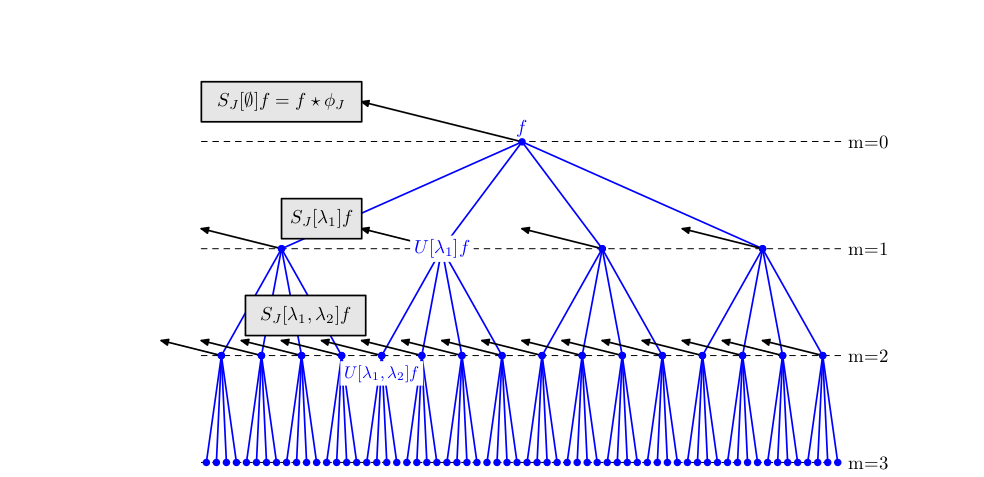
\includegraphics[width=0.8\textwidth]{img/ScatteringPropagator.png}
  \caption{Un PD $U_J$ aplicado a un punto de una señal $f(x)$ calcula $U[\lambda_1]f(x)=|f(x)\ast \psi_{\lambda_1}|$ y como salida a la capa $m=0$ se promedian los coeficientes que han dado $0$ (por tener $2^j<2^-j$) obteniendo como salida $S_J[\emptyset]f(x)=f(x)\ast \phi_{2^J}$ (como se puede ver en la flecha negra). Después se aplica de nuevo $U_J$ a cada coeficiente $U[\lambda_1]f(x)$ del paso anterior ($m=1$) $U[\lambda_1,\lambda2]f(x)$ obteniendo como salida $S_J[\lambda_1]f(x)=U[\lambda_1]f(x) \ast \phi_{2^J}$. Se repite este proceso de manera recursiva para cada coeficiente $U[p]f(x)$ y obteniendo como resultado $S_J[p]f(x)=U[p]f(x) \ast \phi_{2^J}$. }
  \label{fig:scattering_propagator}
\end{figure}


\subsubsection{Diferencias y similitudes con una CNN}


Las operaciones de la transformada de dispersión que hemos descrito siguen la estructura general de la red neuronal convolucional introducida por LeCun \cite{lecun2015deep}, pues se describen las redes convolucionales como una cascada de convoluciones (la transfomada de ondeletas $W[\lambda]$) y capas de "pooling" que usan funciones no lineales (el operador módulo $M[\lambda]$), las cuales se representan en este modelo como módulos de números complejos. También se puede considerar como un operador de \entrecomillado{pooling} la función $\phi_{2^J}$ que se emplea para agregar coeficientes y contruir un operador invariante.

\medskip

\noindent Las redes neuronales convolucionales han sido empleadas con mucho éxito en tareas de reconocimiento de objetos o personas y usan normalmente Kernels que no son predefinidos, sino que se aprenden mediante la técnica de back-propagation al entrenar la red, en cambio, en la modelización que se ha presentado las ondeletas que usamos son prefijadas y no se aprenden.

\medskip

\noindent Siguiendo con las similitudes entre ambos modelos, si $p$ es un camino de longitud $m$, entonces a $S_J[p] f(x)$ se le denomina coeficiente de orden $m$ a escala $2^J$, que en el caso de una CNN,equivaldría al tensor formado por los mapas de activación tras la convolución con el kernel de la capa $m$ de la red. 

\medskip


\subsubsection{Relación con herramientas clásicas de visión por computador}
\noindent Por otro lado, la modelización  con los algoritmos clásicos de visión por computador como \textbf{SIFT}  \cite{DistinctiveImageFeatures} para calcular puntos de interés en imágenes. Así, con la ondeletas apropiadas, los coeficientes de primer orden $S[\lambda_1] f$ serían equivalentes a los coeficientes del algoritmo. De hecho, en el artículo sobre el descriptor DAISY \cite{Daisy} se muestra cómo esos coeficientes son aproximados por $S_J[2^j r] f= | f \ast \psi_{2^j r} | \ast \phi_{2^J}(x)$, dónde $\psi_{2^j r}$ es la derivada parcial de una Gaussiana calculada en imagen de escala $2^j$ de mayor calidad, para 8 rotaciones distintas $r$. El filtro para promediar $\phi_{2^J}$ es un filtro Gaussiano escalado.


\subsubsection{Operador no expansivo.}

\noindent El propagador $U_Jf=\lbrace A_Jf, \left(\left| W[\lambda]f\right|\right)_{\lambda\in\Lambda_J} \rbrace$ es no expansivo, porque la transformada de ondas $W_J$ es unitaria pues cumple las hipótesis de la \autoref{unitario} y el módulo no es expansivo en el sentido de que $||a|-|b||\leq |a-b|$ para cualquier $(a,b)\in \mathbb{C}^2$. Esto es válido tanto si $f$ es real o compleja. Como consecuencia: 

\begin{align*} 
    ||U_J f-U_J h||^2 &= ||A_J f-A_J h||^2+\sum_{\lambda\in\Lambda_J} \left\| |W[\lambda]f|-|W[\lambda]h| \right\|^2 \\
    &\leq \left| \left| W_J f- W_J h \right| \right|^2 \leq ||f-h||^2
\end{align*}

\noindent Al ser $W_J$ unitaria, tomando la función nula $h=0$ y siguiendo el mismo razonamiento anterior, también se comprueba que $||U_J f||=||f||$ por lo que el operador $U_J$ preserva la norma.

\medskip

\noindent Para todo conjunto de caminos $\Omega$, las normas de $S_J[\Omega]f$ y $U[\Omega]f$ son: 

$$\left|\left| S_J[\Omega]f \right|\right|^2=\sum_{p\in\Omega} \left|\left| S_J[p]f\right|\right|^2 \;\; y \;\; \left|\left|U[\Omega]f\right|\right|^2=\sum_{p\in\Omega} \left|\left| U[p]f\right|\right|^2$$

\noindent Como $S_J[\mathcal{P}_J]$ itera en $U_J$, que es no expansivo, la siguiente proposición prueba que $S_J[\Omega]f$ es también no expansivo. 

\begin{proposicion} \label{proposicion::NoExpansiva}
La transformada de dispersión de ventana es no expansiva: 

\begin{equation}
  \forall (f,h)\in L^2(\mathbb{R}^d)^2 \;\; ||S_J[\mathcal{P}_J]f-S_J[\mathcal{P}_J]h|| \leq ||f-h||
\end{equation}
\end{proposicion}

\begin{proof}
Como $U_J$ es no expansiva, partiendo de \eqref{eq::1.5} que nos dice: 
$$U_J U[\Lambda_J^m]=\lbrace S_J[\Lambda_J^m]f,(U[\Lambda_J^{m+1}]f)_{\lambda\in\Lambda_J}\rbrace,$$

se tiene que:

\begin{align*}
    ||U[\Lambda_J^m]f-U[\Lambda_J^m]h||^2 &\geq ||U_J U[\Lambda_J^m]f-U_J U[\Lambda_J^m]h||^2 \\
    & = ||S_J[\Lambda_J^m]f - S_J[\Lambda_J^m]h||^2 + ||U[\Lambda_J^{m+1}]f-U[\Lambda_J^{m+1}]h||^2.
\end{align*}

\medskip

\noindent Si ahora sumamos en $m$ cuando tiende a $\infty$ se obtiene que: 

\begin{align*}
  \sum_{m=0}^{\infty}||U[\Lambda_J^m]f-U[\Lambda_J^m]h||^2 &\geq \sum_{m=0}^{\infty} ||S_J[\Lambda_J^m]f - S_J[\Lambda_J^m]h||^2 + \sum_{m=0}^{\infty} ||U[\Lambda_J^{m+1}]f-U[\Lambda_J^{m+1}]h||^2,\\
\end{align*}

\noindent que equivale a:

\begin{align*}
  \sum_{m=0}^{\infty}||U[\Lambda_J^m]f-U[\Lambda_J^m]h||^2 - \sum_{m=0}^{\infty} ||U[\Lambda_J^{m+1}]f-U[\Lambda_J^{m+1}]h||^2 &\geq \sum_{m=0}^{\infty} ||S_J[\Lambda_J^m]f - S_J[\Lambda_J^m]h||^2\\
\end{align*}

\noindent Si ahora nos fijamos en el lado izquierdo de la desigualdad, se cancelan todos los términos salvo $m=0$, y teniendo en cuenta que $\Lambda^0_J=\emptyset$ queda: 

\begin{align*}
  \sum_{m=0}^{\infty}||U[\Lambda_J^0]f-U[\Lambda_J^0]h||^2 &= \sum_{m=0}^{\infty}||U[\emptyset]f-U[\emptyset]h||^2 = || f - h ||^2 \\
\end{align*}

\noindent Por otro lado, se tiene que

\begin{align*}
  \sum_{m=0}^{\infty} ||S_J[\Lambda_J^m]f - S_J[\Lambda_J^m]h||^2 = ||S_J[\mathcal{P}_J]f - S_J[\mathcal{P}_J]h||^2. \\
\end{align*}

\noindent Luego hemos probado que 

$$||S_J[\mathcal{P}_J]f - S_J[\mathcal{P}_J]h||^2 \leq || f - h ||^2$$

\noindent y por lo tanto que la transfomada de dispersión de ventana es no expansiva. \qedhere
\end{proof}

\subsubsection{Conservación de la norma.}

En la \autoref{ch:seccion12} se obtuvo que cada coeficiente $U[\lambda]f=|f \ast \psi_\lambda|$ capturaba la energía de frecuencia de $f$ en una banda de frecuencia cubierta por $\widehat{\psi}_\lambda$ y propagaba dicha energía a frecuencias decrecientes, este hecho lo demuestra el siguiente teorema, mostrando que toda la energía del propagador de dispersión alncanza la frecuencia mínima $2^J$ y es atrapada por el filtro paso bajo $\phi_ {2^J}$. La energía propagada tiende a $0$ conforme se incrementa la longitud del camino, y el teorema implica que $||S_J[\mathcal{P}_J]f||=||f||$. Esto se aplica también a funciones complejas en caminos negativos.

\medskip

\noindent Para la demostración de la conservación de la norma necesitamos unos resultados previos: 

\begin{lema} \label{lema::Cota_inferior}
  Si $h$ es una funciones tal que $h\geq 0$ entonces $\forall f \in L^2(\mathbb{R}^d)$: 
  
  \begin{equation}
    |f \ast \psi_\lambda | \ast h \geq \sup_{\eta \in \mathbb{R}^d} |f\ast \psi_\lambda \ast h_\eta | \; \; con \; h_\eta=h(x)e^{i\eta x}
  \end{equation}
\end{lema}
  
\begin{proof}
  
  \begin{align*}
      |f \ast \psi_\lambda | \ast h (x) &= \int \left| \int f(v)\psi_\lambda(u-v)dv \right| h(x-u)du \\
      &=\int \left | \int f(v) \psi_\lambda(u-v) e^{i\eta(x-u)} h(x-u) dv \right| du \\
      &\geq \left | \int \int f(v) \psi_\lambda(u-v) e^{i\eta(x-u)} h(x-u) dv du \right| = \\
      &= \left | \int f(v) \int  \psi_\lambda(x-v-u')h(u') e^{i\eta u'}  du' dv \right| \\
      &= \left | \int f(v) \psi_\lambda \ast h_\eta(x-v) dv \right| = |f\ast \psi_\lambda \ast h_\eta|
  \end{align*}

  \noindent Dónde se ha usado el cambio de variabel $u'=x-u$ con $J=1$.
\end{proof}

\noindent A continuación definimos el concepto de \entrecomillado{ondeleta admisible:}
\begin{definicion}
  Una ondeleta de dispersión se dice que es admisible si existe $\eta \in \mathbb{R}^d$ y una función $\rho \geq 0$, con $|\widehat{\rho}(\omega)| \leq |\widehat{\phi}(2\omega)|$ y $\widehat{\rho}(0)=1$, tal que la función: 

\begin{equation}\label{eq::1.6}
  \widehat{\Psi}(\omega)=|\widehat{\rho}(\omega - \eta)|^2 - \sum_{k=1}^{+\infty} k(1-|\widehat{\rho}(2^{-k}(\omega - \eta))|^2)
\end{equation}
  
\noindent satisface: 
\begin{equation} \label{eq::1.7}
  \alpha= \inf_{1\leq|w|\leq2} \sum_{j=-\infty}^{\infty} \sum_{r\in G} \widehat{\Psi} (2^{-j}r^{-1}\omega)|\widehat{\psi}(2^{-j}r^{-1}\omega)|^2>0.
\end{equation}

\end{definicion}

\noindent Con esta definición en mente podemos comprobar que se da el siguiente lema que demuestra que el propagador dispersa la energía progresivamente hacia bajas frecuencias.

\begin{lema} \label{lema::Admisibilidad}
Si \eqref{eq::1.7} se satisface y 

\begin{equation}
  ||f||_w^2=\sum_{j=0}^\infty \sum_{r\in G^+} j ||W[2^j r] f||^2 < \infty
\end{equation}

\noindent Entonces se tiene: 

\begin{equation}\label{eq::1.9}
  \frac{\alpha}{2}||U[\mathcal{P_J}]f||^2 \geq \max (J+1,1) ||f||^2 + ||f||_w^2.
\end{equation}

\end{lema}

\medskip

\noindent La demostración de lema se encuentra en el apéndice A de \cite{GroupInvariantScattering}.

\medskip

\noindent Con todos estos resultados podemos presentar el principal teorema de esta sección, que nos dará como resultado la preservación de la norma del operador de ventana:


\begin{teorema} \label{teoremaOndeletasAdmisibles}
\noindent Si las ondeletas son admisibles, entonces para toda $f\in L^2(\mathbb{R}^d)$
\begin{equation}
  \lim_{m\rightarrow\infty} ||U[\Lambda_J^m]f||^2=\lim_{m\rightarrow\infty} \sum_{n=m}^{\infty} ||S_J[\Lambda_J^n]f||^2=0
\end{equation}

y

\begin{equation}
  ||S_J[\mathcal{P_J}]f||=||f||
\end{equation}

\end{teorema}

\begin{proof}
  Esta demostración tiene dos partes, la primera consistirá en demostrar que la condición \eqref{eq::1.6} implica que $\lim_{m\rightarrow \infty} ||U[\Lambda_J^m]f||^2=0$. 
  
  \medskip

  \noindent La clave de esto reside en el \autoref{lema::Cota_inferior}, que nos da una cota inferior de $|f\ast\psi_\lambda|$ convolucionada con una función positiva. La clase de funciones para las que $||f||_w < \infty$ es una clase logarítmica de Sobolev correspondiente a funciones que tienen un módulo promedio continuo en $L^2(\mathbb(R)^d)$. Como 

  $$ || U[\mathcal{P}_J]f ||^2= \sum_{m=0}^{+\infty} ||U[\Lambda_J^m]f||^2,$$

  \noindent si $||f||_w < \infty$ entonces \eqref{eq::1.9} implica que $\lim_{m\rightarrow\infty}||U[\Lambda_J^m]f||= 0$. Este resultado se extiende en $L^2(\mathbb{R}^d)$ por densidad. Como $\phi \in L^1(\mathbb{R}^d)$ y $\widehat{\phi}(0)=1$, cualquier $f\in L^2(\mathbb{R}^d)$ satisface $\lim_{n\rightarrow - \infty} ||f-f_n||=0$, dónde $f_n=f \ast \phi_{2^n}$ y $\phi_{2^n}=2^{-nd} \phi(2^{-n}x)$. Se demuestra por tanto que $\lim_{m\rightarrow \infty} ||U[\Lambda_J^m]f_n||=0$ viendo que $||f_n||_w < \infty$. De hecho, 


  \begin{align*}
      ||W[2^jr]f_n||^2 &= \int |\widehat{f}(\omega)|^2 |\widehat{\phi}(2^n \omega)|^2 |\widehat{\psi}(2^{-j}r^{-1}\omega)|^2 d\omega \\
      &\leq C 2^{-2n-2j} \int |\widehat{f}(\omega)|^2 d\omega,
  \end{align*}

  \noindent porque $\psi$ hay un momento en que desaparece entonce $|\widehat{\psi}(\omega)=O(|\omega|)$, y las derivadas de $\phi$ están en $L^1(\mathbb{R}^d)$ luego $|\omega||\widehat{\phi}\omega|$ están acotadas. Por lo que se tiene que $||f_n||_w < \infty$.

  \medskip

  \noindent Como $U[\Lambda^m]$ es no expansiva, $||U[\Lambda_J^m]f-U[\Lambda_J^m]f_m|| \leq ||f - f_n||$, por lo que 

  $$||U[\Lambda_J^m]f|| \leq || f-f_n|| + ||U[\Lambda_J^m]f_n||.$$

  \noindent Como $\lim_{n\rightarrow -\infty}||f-f_n||=0$ y $\lim_{m\rightarrow\infty}||U[\Lambda_J^m]f_n||=0$ tenemos que 

  $$\lim_{m\rightarrow\infty} ||U[\Lambda_J^m]f||^2=0$$

  \noindent para toda $f \in L^2(\mathbb{R}^d)$. 

  \medskip

  \noindent \textbf{En segundo lugar} vamos a ver que las siguientes expresiones son equivalentes: 
  \begin{align*}
    \lim_{m\rightarrow \infty} ||U[\Lambda_J^m]f||^2=0 \iff \lim_{m\rightarrow\infty} \sum_{n=m}^{\infty} ||S_J[\Lambda_J^n]f||^2=0 \iff ||S_J[\mathcal{P_J}]f||^2 = ||f||
  \end{align*}

  En primer lugar probamos que 
  $$\lim_{m\rightarrow \infty} ||U[\Lambda_J^m]f||^2=0 \iff \lim_{m\rightarrow\infty} \sum_{n=m}^{\infty} ||S_J[\Lambda_J^n]f||^2=0$$
  
  \noindent Como $||U_J h||=||h|| \; \forall h \in L^2(\mathbb{R}^d)$ y $U_J U[\Lambda_J^n]f=\lbrace S_J[\Lambda_J^n]f,U[\Lambda_J^{n+1}]\rbrace$,

 \begin{equation} \label{eq::1.8}
  ||U[\Lambda_J^n]f||^2=||U_JU[\Lambda_J^n]f||^2=||S_J[\Lambda_J^n]f||^2+||U[\Lambda_J^{n+1}]f||^2. 
 \end{equation}

  \noindent Sumando en $m\leq n < \infty$ se obtiene : 
  
  \begin{align*}
    \sum_{n=m}^\infty ||U[\Lambda_J^n]f||^2=&\sum_{n=m}^\infty ||S_J[\Lambda_J^n]f||^2 + \sum_{n=m}^\infty||U[\Lambda_J^{n+1}]f||^2 \\
    \Big\Updownarrow \\
    \sum_{n=m}^\infty ||U[\Lambda_J^n]f||^2 -& \sum_{n=m}^\infty||U[\Lambda_J^{n+1}]f||^2 =\sum_{n=m}^\infty ||S_J[\Lambda_J^n]f||^2  \\
  \end{align*}
  
  \noindent En el término de la izquierda se anulan entre si todos los sumandos salvo $n=m$, luego queda: 

  \begin{align*}
    ||U[\Lambda_J^m]f||^2 =\sum_{n=m}^\infty ||S_J[\Lambda_J^n]f||^2  \\
  \end{align*}
  \noindent Y tomando límites cuando $m\rightarrow \infty$
  \begin{align*}
    \lim_{m\rightarrow \infty}||U[\Lambda_J^m]f||^2 =\lim_{m\rightarrow \infty}\sum_{n=m}^\infty ||S_J[\Lambda_J^n]f||^2  \\
  \end{align*}
  \noindent Llegados a este punto se puede apreciar claramente que
  
  $$Si \; \; \lim_{m\rightarrow \infty} ||U[\Lambda_J^m]f||^2=0 \implies \lim_{m\rightarrow\infty} \sum_{n=m}^{\infty} ||S_J[\Lambda_J^n]f||^2=0$$

  \noindent Y el recíproco también es cierto, luego ambas expresiones son equivalentes.

  \medskip

  \noindent Por otro lado, sumando en \eqref{eq::1.8} para $0\leq n < m$ se obtine:

  \begin{align*}
    \sum_{n=0}^{m-1} ||U[\Lambda_J^n]f||^2=&\sum_{n=0}^{m-1} ||S_J[\Lambda_J^n]f||^2 +\sum_{n=0}^{m-1}||U[\Lambda_J^{n+1}]f||^2 \\
    \Big\Updownarrow \\
    \sum_{n=0}^{m-1} ||U[\Lambda_J^n]f||^2 -& \sum_{n=0}^{m-1}||U[\Lambda_J^{n+1}]f||^2 = \sum_{n=0}^{m-1} ||S_J[\Lambda_J^n]f||^2.  \\
  \end{align*}
  
  \noindent En el término de la izquierda se anulan entre si todos los sumandos salvo $n=0$, y teniendo en cuenta que $f=U[\Lambda_J^0]f$ queda:
  
  \begin{equation}
    ||f||^2=\sum_{n=0}^{m-1} ||S_J[\Lambda_J^n]f||^2 + ||U[\Lambda_J^m]f||^2.
  \end{equation}

  \noindent Si ahora tomamos límite cuando $m\rightarrow \infty$ obtenemos: 
  \begin{align*}
    \lim_{m\rightarrow \infty}||f||^2 =\lim_{m\rightarrow \infty}\sum_{n=0}^{m-1} ||S_J[\Lambda_J^n]f||^2 &+ \lim_{m\rightarrow \infty} ||U[\Lambda_J^m]f||^2  \\
    \Big\Updownarrow \\
    ||f||^2 =\sum_{n=0}^{\infty} ||S_J[\Lambda_J^n]f||^2 &+ \lim_{m\rightarrow \infty} ||U[\Lambda_J^m]f||^2  \\
    \Big\Updownarrow \\
    ||f||^2 =||S_J[\mathcal{P_J}]f||^2 &+ \lim_{m\rightarrow \infty} ||U[\Lambda_J^m]f||^2.  \\
  \end{align*}

  \noindent De manera que se puede apreciar claramente que  
  \begin{align*}
    ||f||^2 =||S_J[\mathcal{P_J}]f||^2 + \lim_{m\rightarrow \infty} ||U[\Lambda_J^m]f||^2  = ||S_J[\mathcal{P_J}]f||^2 \iff \lim_{m\rightarrow \infty} ||U[\Lambda_J^m]f||^2=0. \\
  \end{align*}

  \noindent Con lo que queda demostrado el teorema \qedhere
\end{proof}

\subsubsection{Conclusiones extraidas del teorema}
\noindent La demostración muestra que el propagador dispersa la energía progresivamente a frecuencias menores. La energía de $U[p]f$ se concentra principalmente en los caminos de frecuencia decrecientes $p=(\lambda_k)_{k\leq m}$ para los que $|\lambda_{k+1}|<|\lambda_k|$.


\medskip

\noindent El decrecimiento de $\sum_{n=m}^\infty || S_J[\Lambda_J^n]f||^2$ nos sugiere que podemos descartar todos los caminos de longitud mayor que un cierto $m>0$. De hecho, en tareas de tratamiento de imágenes y audio el decrecimiento numérico de $||S_J[\Lambda_J^n]f||^2$ puede llegar a ser exponencial, lo que conlleva a que en problemas de clasificación, por ejemplo, el de camino se liminte a $m=3$.

\medskip

\noindent El teorema además requiere de una transformada de ondeleta unitaria y admisible que satisfaga la condición de Littlewood-Paley $\beta \sum_{(j,r)\in \mathbb{Z}\times G}|\widehat{\psi}(2^jr\omega)|^2=1$. 

\medskip

\noindent Debe también existir una función $\rho \geq 0$ y un $\eta \in \mathbb{R}^d$ con $|\widehat{\rho}(\omega)|\leq |\widehat{\phi}(2\omega)|$ tal que: 

$$\sum_{(j,r)\in\mathbb{Z}\times G}|\widehat{\psi}(2^jr\omega)|^2|\widehat{\rho}(2^jr\omega-\eta)|^2$$

\noindent sea suficientemente grande para que $\alpha>0$. Esto se puede obtener como se indica en $(2.3)$, con $\psi(x)=e^{i\eta x}\Theta(x)$ y de hecho $\widehat{\psi}=\widehat{\Theta}(\omega-\eta)$, dónde $\widehat{\Theta}$ y $\widehat{\rho}$ tienen su energía concentrada en los mismos dominos de frecuencia, que son bajos.

\section{Invarianza por Traslaciones} \label{ch:seccion14}

\noindent Hasta ahora hemos definido el propagador de dispersión y hemos visto algunas propiedades como la conservación de la norma de la señal $f$. No obstante, aún quedan por demostrar propiedades que son esenciales como son la invaianza por traslaciones o la estabilidad bajo la acción de difeomorfismos. En esta sección nos centraremos en el estudio de la invarianza por traslaciones.

\subsection{No expansividad del operador de ventana en conjuntos de caminos}
Vamos a demostrar en primer lugar que $||S_J[\overline{\mathcal{P}}_J] f- S_J[\overline{\mathcal{P}}_J] h ||$ es no expansiva cuando se incrementa $J$, y que de hecho converge cuando $J \rightarrow \infty$. Esto define una distancia límite que como veremos a continuación es invariante por traslaciones.

\medskip

\begin{proposicion}
\noindent Para todo $(f,h) \in L^2(\mathbb{R}^d)^2$ y $J\in \mathbb{Z}$, 

\begin{equation} \label{eq::1.10}
  || S_{J+1} [\mathcal{P}_{j+1}]f- S_{J+1}[\mathcal{P}_{J+1}]h || \leq ||S_J[\mathcal{P}_J]f - S_J[\mathcal{P}_J]h || 
\end{equation}

\end{proposicion}

\begin{proof}

\noindent En primer lugar, vamos a transformar la condición que queremos demostrar en \eqref{eq::1.10} en otra equivalente y que será más fácil de probar.

\medskip

\noindent Si recordamos la definición de $\mathcal{P}_J$, era un conjunto de caminos finitos $p=(\lambda_1,...,\lambda_m)$ tal que $\lambda_k\in\Lambda_J$ y $|\lambda_k|=2^{jk}>2^{-J}$. Luego todo camino $p' \in \mathcal{P}_{J+1}$, puede ser unívocamente escrito como una extensión de un camino $p\in \mathcal{P}_J$ dónde $p$ es el prefijo más grande de $p'$ que pertenece a $\mathcal{P}_J$, y $p'=p+q$ para algún $q\in \mathcal{P}_{J+1}$. De hecho, podemos definir el conjunto de todas las extensiones de $p\in \mathcal{P}_J$ en $\mathcal{P}_{J+1}$ como: 

\begin{equation}
  \mathcal{P}_{J+1}^{p}={p} \cup {p+2^{-J}r+p''}_{r\in G^{+},p''\in \mathcal{P}_{J+1}}
\end{equation}

Esto define una partición disjunta de $\mathcal{P}_{J+1}=\cup_{p \in \mathcal{P}_J} \mathcal{P}_{J+1}^{p}$. Y deberíamos probar que dichas extensiones son no expansivas,

\begin{equation}\label{eq::1.11}
  \sum_{p' \in \mathcal{P}_{J+1}^p} || S_{J+1}[p']f-S_{J+1}[p']h||^2 \leq ||S_{J}[p]f-S_J [p]h||^2.
\end{equation}

\noindent Finalmente, si nos fijamos, la condición \eqref{eq::1.11} equivale a \eqref{eq::1.10} sumando en todo $p\in \mathcal{P}_J$, luego probando \eqref{eq::1.11} tendríamos el resultado que buscamos. 


\medskip


\noindent Para ello vamos a necesitar el siguiente lema:

\begin{lema}
  Para Ondeletas que satisfacen la propiedad \autoref{unitario}, para toda función \textbf{real} $f\in L^2(\mathbb{R}^d)$ y todo $q \in \mathbb{Z}$ se verifica: 

  $$\sum_{-q\geq l > -J} \sum_{r \in G^+} || f \ast \psi_{2^lr}||^2 + || f \ast \phi_{2^J}||^2 = || f \ast \phi_{2^q} ||^2$$

\end{lema}

\begin{proof}

  \noindent En primer lugar vamos a ver que de \autoref{unitario} se deduce la siguiente expresión: 

  $$|\widehat{\phi}(2^J \omega)|^2 + \sum_{-q\geq l > -J} \sum_{r \in G^+}|\widehat{\psi}(2^{-l}r^{-1} \omega)|^2=|\widehat{\phi}(2^q \omega) |^2$$

  \noindent Para ello, de la expresión

  \begin{align*}
    \frac{1}{2} \sum_{j=-\infty}^\infty \sum_{r \in G} |\widehat{\psi}(2^{-j}r^{-1}\omega)|^2=1 & \; \; y
    \;\;|\widehat{\phi}(\omega)|^2= \frac{1}{2} \sum_{j=-\infty}^0 \sum_{r\in G} |\widehat{\psi}(2^{-j}r^{-1}\omega)|^2,
  \end{align*}

  \noindent se tiene de la misma forma que vimos en la demostración del teorema que:

  $$\forall J \in \mathbb{Z} \; \; \; \left|\widehat{\phi}\left(2^J\omega\right)\right|^2 + \frac{1}{2} \sum_{j>-J,r\in G}\left|\widehat{\psi}\left(2^{-j}r^{-1}\omega\right)\right|^2=1. $$

  \noindent Y partiendo el sumatorio obtenemos que: 

  $$\left|\widehat{\phi}\left(2^J\omega\right)\right|^2 + \frac{1}{2}  \sum_{-q \geq j >-J,r \in G}\left|\widehat{\psi}\left(2^{-j}r^{-1}\omega\right)\right|^2= \frac{1}{2} \sum_{j>-q,r \in G}\left|\widehat{\psi}\left(2^{-j}r^{-1}\omega\right)\right|^2=|\widehat{\phi}(2^q \omega)|^2$$
  
  \noindent Ahora multiplicamos en la expresión anterior por $|\widehat{f}(\omega)|^2$, 
  
  $$\left|\widehat{f}(\omega)\right|^2 \left|\widehat{\phi}\left(2^J\omega\right)\right|^2 + \frac{1}{2} \sum_{-q \geq j >-J,r \in G} \left|\widehat{f}(\omega)\right|^2 \left|\widehat{\psi}\left(2^{-j}r^{-1}\omega\right)\right|^2=\left|\widehat{f}(\omega)\right|^2 \left|\widehat{\phi}(2^q \omega)\right|^2.$$

  \noindent Integramos en $\omega$, 

  $$\int \left|\widehat{f}(\omega)\right|^2 \left|\widehat{\phi}\left(2^J\omega\right)\right|^2 d\omega + \frac{1}{2} \sum_{-q \geq j >-J,r \in G} \int \left|\widehat{f}(\omega)\right|^2 \left|\widehat{\psi}\left(2^{-j}r^{-1}\omega\right)\right|^2 d\omega=\int \left|\widehat{f}(\omega)\right|^2 \left|\widehat{\phi}(2^q \omega)\right|^2 d\omega.$$

  \noindent Ahora estamos en condiciones de aplicar el \autoref{Teorema::Convolucion}, y nos quedaría que la expresión anterior equivale a: 

  \begin{align*}
    \int \left|(f \ast \phi_{2^J}) (x)\right|^2 dx + \sum_{-q \geq j >-J,r \in G} \int \left|(f \ast \psi_{2^{j}r})(x)\right|^2 dx=\int \left|(f \ast \phi_{2^q}) (x)\right|^2 dx,
  \end{align*}

  \noindent Y teniendo en cuenta que $f$ es real y por lo tanto que $||f \ast \psi_{2^j r}||= ||f \ast \psi_{2^j -r}||$ junto con la defnición de la norma de $L^2(\mathbb{R}^d)$, se tiene  

  \begin{align*}
    \sum_{-q\geq l > -J} \sum_{r \in G^+} || f \ast \psi_{2^lr}||^2 + || f \ast \phi_{2^J}||^2 = || f \ast \phi_{2^q} ||^2
  \end{align*}

\end{proof}


Vamos ahora a usar el lema anterior con la función $g=U[p]f-U[p]h$ junto con que $U[p]f\ast \phi_{2^J}=S_J[p]f$. De esta forma se tiene:

$$||g \ast \phi_{2^{J+1}} ||^2 + \sum_{r\in G^+} || g\ast \psi_{2^{-J}r} ||^2=||g \ast \phi_{2^J}||^2.$$

\noindent Así, sustituyendo el valor de $g$ por el que hemos definido antes y aplicando la propiedad distributiva de la convolución:

\begin{align*}
  ||U[p]f \ast \phi_{2^J} -U[p]h \ast \phi_{2^J}||^2 = &||U[p]f \ast \phi_{2^{J+1}} - U[p]h \ast \phi_{2^{J+1}} ||^2 \\
  & + \sum_{r\in G^+} || U[p]f\ast \psi_{2^{-J}r} -U[p]h \ast \psi_{2^{-J}r}||^2.
\end{align*}

\noindent Y esto equivale a

\begin{align*}
  ||S_{J}[p]f-S_J[p]h||^2 = &|| S_{J+1}[p]f-S_{J+1}[p]h||^2 \\
  & + \sum_{r\in G^+} || U[p]f\ast \psi_{2^{-J}r} -U[p]h \ast \psi_{2^{-J}r}||^2.
\end{align*}

\noindent Aplicando ahora la propiedad de la norma de que $\left|\left|a - b \right|\right| \geq \left|\left| |a| - |b| \right|\right|$. Y como $$|U[p]f\ast\psi_{2^{-J}r}|=U[p+2^{-J}r]f$$ se concluye que:

\begin{align*}
    ||S_{J}[p]f-S_J[p]h||^2 \geq & || S_{J+1}[p]f-S_{J+1}[p]h||^2 \\
    & + \sum_{r\in G^+} ||U[p+2^{-J}r]f-U[p+2^{-J}r]h||^2.
\end{align*}


\noindent Como $S_{J+1}[\mathcal{P}_{J+1}]U[p+2^{-J}r]f=\lbrace S_{J+1} [p+2^{-J}r+p'']\rbrace_{p''\in\mathcal{P}_{J+1}}$  y $S_{J+1}[\mathcal{P}_{J+1}]f$ es no expansiva por \autoref{proposicion::NoExpansiva}, esto implica que

\begin{align*}
    ||S_{J}[p]f - S_J[p]h||^2 \geq & ||S_{J+1}[p]f-S_{J+1}[p]h||^2 \\
    & + \sum_{p''\in \mathcal{P}_{J+1}} \sum_{r\in G^+} || S_{J+1}[p+2^{-J}r+p'']f- S_{J+1}[p+2^{-J}r+p'']h||^2,
\end{align*}

\noindent y en particular

\begin{align*}
  ||S_{J}[p]f - S_J[p]h||^2 \geq & \sum_{p''\in \mathcal{P}_{J+1}} \sum_{r\in G^+} || S_{J+1}[p+2^{-J}r+p'']f- S_{J+1}[p+2^{-J}r+p'']h||^2,
\end{align*}

\noindent que demuestra \eqref{eq::1.11}. \qedhere
\end{proof}


\subsection{Invarianza por traslaciones}

\noindent Esta proposición anterior nos demuestra que $||S_J[\mathcal{P}_J]-S_J[\mathcal{P}_J]h||$ es positivo y no creciente cuando $J$ se incrementa, y de hecho converge. Como $S_J[\mathcal{P}_J]$ es no expansiva, el límite tampoco: 

$$\forall (f,h)\in L^2(\mathbb{R}^d)^2 \lim_{J\rightarrow\infty} ||S_J[\mathcal{P}_J]f-S_{J}[\mathcal{P}_J]h|| \leq ||f-h||.$$

\medskip

\noindent Para ondeletas de dispersión admisibles que satisfacen \eqref{eq::1.7}, El \autoref{teoremaOndeletasAdmisibles} nos demuestra que $||S_J[\mathcal{P}_J]f||=||f||$ entonces $\lim_{J\rightarrow\infty}||S_J[\mathcal{P}_J]f||=||f||$. El siguiente teorema demuestra que el límite es invariante por traslaciones, pero para la demostración del teorema necesitaremos de un resultado auxiliar: 

\begin{lema} \label{lema::constante}
  Existe una constante $C$ tal que para todo $\tau \in \C^2(\mathbb{R}^d)$ con $||\nabla \tau ||_\infty \leq \frac{1}{2}$ se tiene que 
  
  $$||L_\tau A_J f - A_J f|| \leq C ||f||2^{-J}||\tau||_{\infty}.$$
\end{lema}

\begin{proof}

  \noindent En esta prueba, al igual que en otras cotas superiores para normas, vamos a necesitar el Lema de Schur \cite{SchurLemma}. De esta manera, el Lema de Schur nos recuerda que para cualquier operador $Kf(x)=\int f(u)k(x,u)du$ se tiene 

  $$\int |k(x,u)| dx \leq C,$$

  \noindent y además 

  $$\int |k(x,u)|du \leq C \implies ||K||\leq C.$$

  \noindent Dónde $||K||$ es la norma en $L^2(\mathbb{R}^d)$ de $K$.

  \medskip

  El operador norma de $k_J=L_\tau A_J - A_J$ se calcula aplicando el lema de Schur a su kernel,

  $$k_J(x,u)=\phi_{s^J}(x-\tau(x)-u)-\phi_{2^J}(x-u).$$

  \noindent Si nos fijamos en la expresión anterior, cuando $x=0=u$ se tiene que: 

  $$k_J(0,0)=\phi_{2^J}(0)-\phi_{2^J}(0)=0.$$

  \noindent Si ahora calculamos su serie de primer orden de Taylor centrado en el $(0,0)$ se obtiene: 

  $$k_J=k_J(0,0)+\int_0^1 \nabla \phi_{2^J} (x-t\tau(x)-u)\tau(x). dt$$

  \noindent Si ahora calculamos el módulo obtenemos que:

  \begin{align*}
    |k_J|&=|k_J(0,0)+\int_0^1 \nabla \phi_{2^J} (x-t\tau(x)-u)\tau(x) dt| \\
    &\leq |k_J(0,0)|+\left|\int_0^1 \nabla \phi_{2^J} (x-t\tau(x)-u)\tau(x) dt \right| \\
    & \leq \left|\int_0^1 \nabla \phi_{2^J} (x-t\tau(x)-u)\tau(x) dt \right| \\ 
    & \leq \int_0^1 \left| \nabla \phi_{2^J} (x-t\tau(x)-u)\tau(x)  \right|dt= |\tau(x)|\int_0^1 \left| \nabla \phi_{2^J} (x-t\tau(x)-u)\right|dt  \\ 
    & \leq ||\tau(x)||_\infty \int_0^1 \left| \nabla \phi_{2^J} (x-t\tau(x)-u)\right|dt.
  \end{align*}

  \noindent Si ahora integramos en $u$ y aplicamos el teorema de Fubini para itercambiar las integrales del lado derecho de la desigualdad obtenemos:

  \begin{align*}
    \int |k_J| du &\leq ||\tau(x)||_\infty \int \int_0^1 \left| \nabla \phi_{2^J} (x-t\tau(x)-u)\right|dt \; du = ||\tau(x)||_\infty \int_0^1 \int  \left| \nabla \phi_{2^J} (x-t\tau(x)-u)\right| du \; dt. 
  \end{align*}

  \noindent por otro lado, vamos a comprobar que 
  $$\nabla\phi_{2^J}(x)=2^{-dJ-J} \nabla \phi(2^{-J}x).$$

  \noindent Para ello debemos recordar que $\phi_{2^J}(x)=2^{-dJ}\phi(2^{-J}x)$ luego

  \begin{align*}
    \nabla \phi_{2^J}(x) &= \nabla(2^{-dJ}\phi(2^{-J}x)) \\
    &= 2^{-dJ} \nabla(\phi(2^{-J}x)).
  \end{align*}

  \noindent Si nos fijamos, debido a que x está multiplicado por $2^{-J}$ en cada componente del vector, siempre que derivemos con respecto a alguna componente, vamos a poder sacar como factor común $2^{-J}$ por lo tanto:

  \begin{align*}
    \nabla \phi_{2^J}(x) = 2^{-dJ-J} \nabla(\phi(2^{-J}x)).
  \end{align*}

  \noindent De esta forma, realizando un cambio de variable tendríamos: 

  \begin{align*}
    \int |k_J| du &\leq ||\tau(x)||_\infty  2^{-dJ-J} \int \left| \nabla \phi (2^J u')\right|du' \\
    & = 2^{-J} ||\tau(x)||_\infty ||\nabla\phi||_1. 
  \end{align*}

  \noindent Si ahora realizamos el mismo procedimiento integrando en $x$ en vez de en $u$ tenemos que 

  \begin{align*}
    \int |k_J(x,u)| dx &\leq ||\tau(x)||_\infty \int_0^1 \int \left| \nabla \phi_{2^J} (x-t\tau(x)-u)\right| dx \; dt
  \end{align*}

  \noindent Si ahora aplicamos el cambio de variable $v=x - t\tau(x)$ y calculamos su Jacobiano

  \begin{align*}
    Jv& =J(x-t\tau(x))=J(x)-J(t\tau(x)) \\
    & = Id - tJ(\tau(x)) \\
    & = Id - t\nabla \tau(x).
  \end{align*}

  \noindent Vamos a buscar una cota para el determinante del Jacobiano

  \begin{align*}
    |J| & =(1-t\tau(x))^d \\
    & \geq (1-||\tau||_\infty)^d \\
    & \geq 2^{-d}.
  \end{align*}

  \noindent Aplicando ahora el cambio de variable a la integral

  \begin{align*}
    \int |k_J(x,u)| dx &\leq ||\tau(x)||_\infty 2^d \int_0^1 \int \left| \nabla \phi_{2^J} (v-u)\right| dv \; dt \\
    &= 2^{-J} ||\tau||_\infty ||\nabla \phi ||_1 2^{d}.
  \end{align*}

  \noindent De las dos cotas superiores obtenidas esta es la mayor, por lo que aplicamos el lema de Schur a esta y terminamos la demostración del lema

  $$ ||L_{\tau} A_J - A_J || \leq 2^{-J+d} ||\nabla \phi ||_1 ||\tau||_\infty. $$
\end{proof}


\noindent Con esto ya tenemos todas las herramientas necesarias para enunciar y demostrar el teorema central de esta sección, aquel que nos garantiza que el operador que estamos construyendo que modeliza una red neuronal convolucional es invariante a traslaciones.

\begin{teorema} \label{invarianzaTraslaciones}
Para ondeletas de dispersión admisibles se tiene que 

$$\forall f \in L^2(\mathbb{R}^d), \; \forall c\in \mathbb{R}^d \;\;\; \lim_{J\rightarrow \infty}||S_J[\mathcal{P}_J] f-S_J[\mathcal{P}_J] L_cf||=0$$
\end{teorema}

\begin{proof}

\noindent Fijamos $f\in L^2(\mathbb{R}^d)$. Teniendo en cuenta la conmutatividad $S_J[\mathcal{P}_J] L_cf = L_cf S_J[\mathcal{P}_J]$ y la definición $S_J[\mathcal{P}_J]f=A_J U[\mathcal{P}_J]f$,

\begin{align*}
    ||S_J[\mathcal{P}_J] L_cf - S_J[\mathcal{P}_J]f || &= ||L_c A_J U[\mathcal{P}_J]f - A_J U[\mathcal{P}_J]f|| \\
    &\leq ||L_c A_J - A_J|| ||U[\mathcal{P}_J]f||.
\end{align*}

\medskip

\noindent Si ahora aplicamos el \autoref{lema::constante} con $\tau=c$, se tiene que $||\tau||_\infty=|c|$ y además

$$||L_c A_J - A_J|| \leq C 2^{-J} |c|.$$

\noindent Y si tenemos en cuenta esto en la expresión anterior nos da que: 

\begin{align*}
  ||S_J[\mathcal{P}_J] L_cf - S_J[\mathcal{P}_J]f || & \leq ||L_c A_J - A_J|| ||U[\mathcal{P}_J]f|| \\
  & \leq C 2^{-J} |c| ||U[\mathcal{P}_J]f||
\end{align*}

\noindent Como la admisibilidad de la condición \eqref{eq::1.7} se satisface, \autoref{lema::Admisibilidad} se demuestra en \eqref{eq::1.9} que para $J>1$

$$\frac{\alpha}{2}||U[\mathcal{P}_J]f||^2 \leq (J+1)||f||^2+||f||^2_w.$$

\noindent Y de esta expresión podemos sacar una cota superior para $||U[\mathcal{P}_J]f||$: 

\begin{align*}
  ||U[\mathcal{P}_J]f||^2 \leq ((J+1)||f||^2+||f||^2_w) 2 \alpha^{-1}
\end{align*}

\noindent Si $||f||_w < \infty$ entonces elevando al cuadrado en la desigualdad de antes tenemos

$$||S_J[\mathcal{P}_J] L_cf - S_J[\mathcal{P}_J]f ||^2 \leq ((J+1)||f||^2+||f||_w^2)C^2 2 \alpha^{-1} 2^{-2J} |c|^2,$$

\noindent y tomando límite en ambo lados cuando $J\rightarrow \infty$ tenemos que 

\begin{align*}
  \lim_{J\rightarrow \infty} ||S_J[\mathcal{P}_J] L_cf - S_J[\mathcal{P}_J]f ||^2 &\leq \lim_{J\rightarrow \infty} ((J+1)||f||^2+||f||_w^2)C^2 2 \alpha^{-1} 2^{-2J} |c|^2 \\
  &= 0.
\end{align*}

\noindent Luego $\lim_{J\rightarrow\infty}||S_J[\mathcal{P}_J] L_cf - S_J[\mathcal{P}_J]f ||=0$.

\medskip

\noindent Finalmente vamos a probar ahora que el límite anterior se da $\forall f \in L^2(\mathbb{R}^d)$, con un argumento similar al de la prueba del \autoref{teoremaOndeletasAdmisibles}. Cualquier $f\in L^2(\mathbb{R}^d)$ se puede escribir como el límite de una sucesión de funciones $\lbrace f_n \rbrace_{n\in\mathbb{N}}$ con $||f_n||_w < \infty$, y como $S_J[\mathcal{P}_J]$ es no expansivo y $L_c$ es unitario, se puede verificar que 

$$||L_c S_J[\mathcal{P}_J]f-S_J[\mathcal{P}_J]f|| \leq ||L_c S_J [\mathcal{P}_J]f_n -S_J[\mathcal{P}_J]f_n|| + 2||f-f_n||.$$

\noindent Haciendo tender $n \rightarrow \infty$ se prueba que $\lim_{J\rightarrow \infty}||S_J[\mathcal{P}_J] f-S_J[\mathcal{P}_J] L_cf||=0$ con lo que acaba la demostración. \qedhere
\end{proof}



































\begin{itemize}
  \item La  memoria  debe  realizarse  con  un  procesador  de  texto  científico,  preferiblemente (La)TeX.
  \item La portada  debe contener  el  logo  de  la UGR,  incluir  el  título del TFG, el nombre del estudiante y especificar el grado, la facultad y el curso actual.
  \item La contraportada contendrá además el nombre del tutor o tutores.
  \item La memoria debe necesariamente incluir:
    \begin{itemize}
      \item un índice detallado de capítulos y secciones,
      \item un resumen amplio en inglés del trabajo realizado (se recomienda entre 800 y 1500 palabras),
      \item una introducción en la que se describan claramente los objetivos previstos inicialmente en la propuesta de TFG, indicando si han sido o no alcanzados, los antecedentes importantes para el desarrollo, los resultados obtenidos, en su caso y las principales fuentes consultadas,
      \item una bibliografía final que incluya todas las referencias utilizadas.
    \end{itemize}
  \item Se recomienda que la extensión de la memoria sea entre 30 y 60 páginas, sin incluir posibles apéndices.
\end{itemize}

Para generar el pdf a partir de la plantilla basta compilar el fichero \texttt{libro.tex}. Es conveniente leer los comentarios contenidos en dicho fichero pues ayudarán a entender mejor como funciona la plantilla. 

La estructura de la plantilla es la siguiente\footnote{Los nombres de las carpetas no se han acentuado para evitar problemas en sistemas con Windows}: 
\begin{itemize}
  \item Carpeta \textbf{preliminares}: contiene los siguientes archivos
    \begin{description}
      \item[\texttt{dedicatoria.tex}] Para la dedicatoria del trabajo (opcional)
      \item[\texttt{agradecimientos.tex}] Para los agradecimientos del trabajo (opcional)
      \item[\texttt{introduccion.tex}] Para la introducción (obligatorio)
      \item[\texttt{summary.tex}] Para el resumen en inglés (obligatorio)
      \item[\texttt{tablacontenidos.tex}] Genera de forma automática la tabla de contenidos, el índice de figuras y el índice de tablas. Si bien la tabla de contenidos es conveniente incluirla, el índice de figuras y tablas es opcional. Por defecto está desactivado. Para mostrar dichos índices hay que editar este fichero y quitar el comentario a \verb+\listoffigures+ o \verb+\listoftables+ según queramos uno de los índices o los dos. En este archivo también es posible habilitar la inclusión de un índice de listados de código (si estos han sido incluidos con el paquete \texttt{listings})
  \end{description}
  El resto de archivos de dicha carpeta no es necesario editarlos pues su contenido se generará automáticamente a partir de los metadatos que agreguemos en \texttt{libro.tex}

  \item Carpeta \textbf{capitulos}: contiene los archivos de los capítulos del TFG. Añadir tantos archivos como sean necesarios. Este capítulo es \texttt{capitulo01.tex}.

  \item Carpeta \textbf{apendices}: Para los apéndices (opcional)
  \item Carpeta \textbf{img}: Para incluir los ficheros de imagen que se usarán en el documento.
  \item Carpeta \textbf{paquetes}: Incluye dos ficheros 
    \begin{description}
      \item[\texttt{hyperref.tex}] para la configuración de hipervínculos al generar el pdf (no es necesario editarlo) 
      \item[\texttt{comandos-entornos.tex}] donde se pueden añadir los comandos y entornos personalizados que precisemos para la elaboración del documento. Contiene algunos ejemplos
    \end{description}
    
  \item Fichero \texttt{library.bib}: Para incluir las referencias bibliográficas en formato \texttt{bibtex}. Son útiles las herramientas \href{https://www.doi2bib.org/}{doi2bib} y \href{https://www.ottobib.com/}{OttoBib} para generar de forma automática el código bibtex de una referencia a partir de su \textsc{doi} o su \textsc{isbn}. Para que una referencia aparezca en el pdf no basta con incluirla en el fichero \texttt{library.bib}, es necesario además \emph{citarla} en el documento usando el comando \verb+\cite+. Si queremos mostrar todos las referencias incluidas en el fichero \texttt{library.bib} podemos usar \verb+\cite{*}+ aunque esta opción no es la más adecuada. Se aconseja que los elementos de la bibliografía estén citados al menos una vez en el documento (y de esa forma aparecerán de forma automática en la lista de referencias).

  \item Fichero \texttt{glosario.tex}: Para incluir un glosario en el trabajo (opcional). Si no queremos incluir un glosario deberemos borrar el comando \verb+% !TeX root = ../libro.tex
% !TeX encoding = utf8

\chapter*{Glosario}
\addcontentsline{toc}{chapter}{Glosario} % Añade el glosario a la tabla de contenidos

La inclusión de un glosario es opcional.

Archivo: \texttt{glosario.tex}

\begin{description} 
  \item[$\mathbb{R}$] Conjunto de números reales.

  \item[$\mathbb{C}$] Conjunto de números complejos.

  \item[$\mathbb{Z}$] Conjunto de números enteros.
\end{description}
\endinput
+ del fichero \texttt{libro.tex} y posteriormente borrar el fichero \texttt{glosario.tex}

   \item Fichero \texttt{libro.tex}: El documento maestro del TFG que hay que compilar con \LaTeX\ para obtener el pdf. En dicho documento hay que cambiar la \emph{información del título del \textsc{tfg} y el autor así como los tutores}.
\end{itemize}

Finalmente y de forma también opcional se puede incluir in índice terminológico. Por defecto dicha opción está desabilitada. Para habilitar la inclusión de dicho índice terminológico basta con quitar los comentarios a las líneas finales de \texttt{libro.tex} y cargar el paquete \texttt{makeindex} en el preámbulo del documento (ver comentarios en \texttt{libro.tex})


\section{Elementos del texto}

En esta sección presentaremos diferentes ejemplos de los elementos de texto básico. Conviene consultar el contenido de \texttt{capitulos/capitulo01.tex} para ver cómo se han incluido.

\subsection{Listas}
En \LaTeX\ tenemos disponibles los siguientes tipos de listas:

Listas enumeradas:
\begin{enumerate}
  \item item 1
  \item item 2
  \item item 3
\end{enumerate}

Listas no enumeradas
\begin{itemize}
  \item item 1
  \item item 2
  \item item 3
  \end{itemize}

Listas descriptivas
\begin{description}
  \item[termino1] descripción 1
  \item[termino2] descripción 2
\end{description}
  
\subsection{Tablas y figuras}

En la \autoref{tb:ejemplo-tabla} o la \autoref{fig:logo-ugr} podemos ver\ldots

\begin{table}[htpb]
  \centering
  \begin{tabular}{ccc} \toprule
    \multicolumn{2}{c}{Agrupados} \\ \cmidrule(r){1-2}
    cabecera & cabecera & cabecera          \\ \midrule
    elemento & elemento & elemento          \\ 
    elemento & elemento & elemento          \\ 
    elemento & elemento & elemento          \\ \bottomrule
  \end{tabular}
  \caption{Ejemplo de tabla}
  \label{tb:ejemplo-tabla}
\end{table}

\begin{figure}[htpb]
  \centering
  
\includegraphics[width=0.8\textwidth]{logo-ugr}
  \caption{Logotipo de la Universidad de Granada}
  \label{fig:logo-ugr}
\end{figure}

\section{Entornos matemáticos}

\begin{teorema}\label{thm:teorema}
Esto es un ejemplo de teorema.
\end{teorema}

\begin{proposicion}
Ejemplo de proposición
\end{proposicion}

\begin{lema}
Ejemplo de lema
\end{lema}

\begin{corolario}
Ejemplo de corolario
\end{corolario}

\begin{definicion}
Ejemplo de definición
\end{definicion}

\begin{observacion}
Ejemplo de observación
\end{observacion}

Y esto es una referencia al \autoref{thm:teorema}. 

Identidad Pitagórica~\eqref{eq:identidad-pitagorica}\index{Identidad pitagórica}
\begin{equation}\label{eq:identidad-pitagorica}
  \cos^2 x + \sin^2 x = 1
\end{equation}

La fórmula de Gauss-Bonnet\index{Gauss-Bonnet!fórmula} para una superficie compacta $S$ viene dada por:
\begin{equation}
  \int_S K = 2\pi\chi(S)
\end{equation}


\section{Bibliografía e índice}

Además incluye varias entradas al índice alfabético mediante el comando \verb+\index+ \index{Leonard!Euler|textbf}


\endinput




\chapter{Modelización Matemática de una Red Neuronal Convolucional} 

\noindent Nuestro primer objetivo será tratar de llegar a la modelización matemática de lo que es una \textbf{CNN}. Para ello, necesitamos definir un operador, que denominaremos \textbf{propagador de dispersión} (PD), que será el que aplicaremos de forma recursiva en una cascada de convoluciones. Explicaremos la problemática de elegir un operador \textit{lipschitz-continuo} bajo la acción de difeomorfismos e \textit{invariante por traslaciones} para evitar problemas como la inestabilidad en altas frecuencias que se producen en las señales bajo la acción de difeomorfismos. 

\medskip

\noindent En segundo lugar,  veremos posibles alternativas para evitar que se produzcan estas inestabilidades mediante el uso de bases de la transformada de ondeletas de \textbf{Littlewood-Paley}. En concreto con esta alternativa obtendremos un operador \textbf{Lipschitz-continuo} bajo la acción de difeomorfismos. 

\medskip

\noindent Después, nuestra tarea será conseguir calcular coeficientes que sean invariantes por traslaciones, y para ello necesitaremos utilizar un operador no lineal como es el módulo. 

\medskip

\noindent Una vez tengamos un operador con todas las propiedades anteriores presentaremos el \textbf{PD}, y será la aplicación en cadena de este operador sobre un \entrecomillado{camino} de frecuencias y rotaciones el que definirá la modelización matemática de una Red Neuronal Convolucional. Todo este capítulo está basado en la investigación de Mallat y sigue como hilo conductor su publicación \cite{GroupInvariantScattering} junto con otros autores que serán citados debidamente.


\section{De Fourier a las ondeletas de Littlewood-Paley}

\subsection{El módulo de la Transformada de Fourier}

\noindent El análisis de Fourier, tradicionalmente, ha jugado un papel fundamental en el procesamiento de señales \cite{DigitalImageProcessing}, por lo que podría parecer un buen punto de partida para la construcción del \textit{propagador de dispersión} emplear la \textbf{transformada de Fourier}, una de las herramientas matemáticas más potentes en este campo. La intuición detrás de su fórmula, es la de representar funciones no periódicas (pero que tienen área finita bajo su gráfica) como la integral de senos y cosenos multiplicados por una función que determina los pesos en cada instante. Formalmente, tiene la siguiente expresión:

\begin{equation}
\widehat{f}(\omega):= \int{f(x)e^{-ix\omega}dx}=\int{f(x)\left[\cos{x\omega} -i\sin{x\omega}\right]dx}.
\end{equation}

\noindent Entre las propiedades más destacables de la transformada encontramos el hecho de que una función se puede recuperar sin pérdida de información a partir de su transformada de Fourier, lo cual nos permite poder trabajar en el \entrecomillado{Dominio de Fourier}\footnote{También llamado \entrecomillado{Dominio de Frecuencia}} ya que al calcular la integral, la función resultante sólo depende de $\omega$ (la frecuencia), y posteriormente pasar de nuevo al dominio original de la función, aplicando la inversa de la transformada sin pérdida de información.

\medskip

\noindent Esto, a priori, es algo atractivo, pues nos permitiría trabajar en un dominio más sencillo y extraer conclusiones que podemos traducir al dominio original de la señal sin pérdida de información. Además, en el estudio de señales se suele emplear el módulo de la transformada de Fourier para evitar fases complejas en el análisis. De esta forma, el operador que vamos a probar en primer lugar es: 

\begin{definicion}
$\Phi(f)=|\widehat{f}|$ módulo de la transformada de Fourier. 
\end{definicion}

\noindent Vamos a comprobar si se trata de un operador válido para nuestro propósito. Para ello necesitamos en primer lugar que sea un operador \textbf{invariante por traslaciones}.

\begin{lema} \label{lema::invarianza_traslaciones}
    El operador $\Phi$ es invariante por traslaciones.
\end{lema}

\begin{proof}
    \noindent Consideramos, para cada $c \in \mathbb{R}^d$, la traslación $L_cf(x)=f(x-c)$. Se tiene que:  
    
    $$\widehat{L_cf}(w)=\int_{\mathbb{R}^d}{L_cf(x) e^{-ixw} dx}=\int_{\mathbb{R}^d}{f(x-c)e^{-ixw}dx}$$
    
    \noindent y realizando el cambio de variable $x-c=y$ se obtiene: 
    
    \begin{align*}
        \int_{\mathbb{R}^d}{f(x-c)e^{-ixw}dx} &= \int_{\mathbb{R}^d}{f(y)e^{-i(y+c)w}dy}= \\      &=\int_{\mathbb{R}^d}{f(y)e^{-iyw}e^{-icw}dy}= \\ &=e^{-icw}\int_{\mathbb{R}^d}{f(y)e^{-iyw}dy}=e^{-icw}\widehat{f}(w)
    \end{align*}
    
    \noindent Por lo que se tiene que $|\widehat{L_cf}(w)|=|e^{-icw}| |\widehat{f}(w)|=|\widehat{f}(w)|$ y entonces $\Phi$ es invariante por traslaciones. \qedhere
\end{proof}

\medskip
    
\noindent Sin embargo, la invarianza por traslaciones no es suficiente. Necesitamos también que nuestro operador sea invariante frente a pequeñas deformaciones (difeomorfismos). De esta forma, diremos que un operador $\Phi(f)$ es estable frente a deformaciones si verifica la Definición \ref{def::Lipschitz_cont}.

\noindent Consideramos la función $\tau(x)\coloneqq \epsilon x$ con $0 < \epsilon << 1$. De esta forma $\|\nabla \tau (x) \|_\infty = \epsilon$ y $\|H\tau(x)\|_\infty=0$. Con esto, la condición de Lipschitz para el módulo de la transfomada de Fourier nos daría la existencia de una constante $c>0$ de modo que la desigualdad que se tendría que cumplir para cada $f \in L^2(\mathbb{R}^d)$ y cada $0 < \epsilon << 1$ sería:


  \begin{equation} \label{eq::lipschitz_condition}
    \|\;|\widehat{f}| -|\widehat{L_\tau f}| \; \| \leq c \|f\| (\|\nabla \tau \|_{\infty} + \|H\tau\|_\infty) = c \|f\| \epsilon.
  \end{equation}

  \noindent Lo que implica encontrar una constante $c\in \mathbb{R}$ que cumpla la desigualdad para cualquier valor de $\epsilon$.Vamos a ver un contraejemplo con una función de una dimensión por simplicidad.

  \medskip

  \noindent Supongamos que tenemos $f(x)=e^{i \xi x}e^{-|x|}$ donde $\xi$ está por determinar. Calculamos ahora $|\widehat{f}|$ y $|\widehat{L_\tau f}|$ teniendo en cuenta que :


  \begin{align*}
    |\widehat{f}(\omega)|&=\left|  \int{f(x)e^{-ix\omega}dx}  \right | \\
    &=\left|  \int{f(x)e^{-ix\omega}dx}  \right | \\
    &=\left|  \int{e^{i \xi x}e^{-|x|}e^{-ix\omega}dx}  \right | \\
    &=\left|  \int{e^{-ix(\xi-\omega)}dx} \right |e^{-|x|} \\
    &=\left|  \int{e^{-|x|}\left[\cos{x(\xi-\omega)} -i\sin{x(\xi-\omega)}\right]dx} \right| \\
  \end{align*}

  \noindent En el último paso podemos descomponer la integral en suma de dos, y para simplificar las operaciones llamamos $\beta=(\xi - \omega)$. Así, aplicando las siguientes fórmulas conocidas para el cálculo de integrales,


  \begin{equation} \label{eq:res_auxiliar_1}
    \int_\mathbb{R} \cos(\beta x) e^{-|x|} dx= \frac{2}{1+\beta^2}
  \end{equation}

  \noindent y 

  \begin{equation}\label{eq:res_auxiliar_2}
    \int_\mathbb{R} \sin(\beta x) e^{-|x|} dx= 0
  \end{equation}

  \noindent a nuestro caso concreto, obtenemos que: 

  \begin{align*}
    |\widehat{f}(\omega)|&=\left|  \int{\cos(x\beta)e^{-|x|} dx} - i \int{\sin(x\beta)e^{-|x|} dx} \right| \\
    &=\frac{2}{1+\beta^2} \\
    &=\frac{2}{1+(\xi - \omega)^2}.
  \end{align*} 

  \noindent Ahora pasamos a calcular $|\widehat{L_\tau f}|$:

  \begin{align*}
    |\widehat{L_\tau f}(\omega)| &= |\widehat{f}((1-\epsilon)\omega)| \\
    &=\left|  \int{f((1-\epsilon)x)e^{-ix\omega}dx}  \right | \\
    &=\left|  \int{e^{i \xi (1-\epsilon) x}e^{-|(1-\epsilon)x|}e^{-ix\omega}dx}  \right |. \\
  \end{align*}

  \noindent Ahora realizamos el siguiente cambio de variable

  \begin{equation}
    \tilde{x}=(1-\epsilon) x \implies x=\frac{\tilde{x}}{1-\epsilon} 
  \end{equation}

  \begin{equation}
  d\tilde{x}=(1-\epsilon) dx \implies dx=\frac{1}{(1-\epsilon)}d\tilde{x}
  \end{equation}

  \noindent y aplicando los cambios a lo que teníamos nos queda

  \begin{align*}
    |\widehat{L_\tau f}(\omega)| 
    &= \frac{1}{(1-\epsilon)}\left|  \int{f((1-\epsilon)x)e^{-ix\omega}dx}  \right | \\
    &=\frac{1}{(1-\epsilon)}\left|  \int{e^{i \xi \tilde{x}}e^{-|\tilde{x}|}e^{-i\frac{\tilde{x}}{(1-\epsilon)}\omega}d\tilde{x}}  \right | \\
    &=\frac{1}{(1-\epsilon)}\left|  \int{e^{i \left[ \frac{(1-\epsilon) \xi - \omega}{(1-\epsilon)}\right]\tilde{x}}e^{-|\tilde{x}|} d\tilde{x}}  \right | \\
    &=\frac{1}{(1-\epsilon)}\left|  \int{e^{i \tilde{\beta}\tilde{x}}e^{-|\tilde{x}|} d\tilde{x}}  \right |. \\
  \end{align*}

  \noindent Como podemos ver, llegamos a una integral que se resuelve de la misma manera que en el caso anterior haciendo uso de \eqref{eq:res_auxiliar_1} y \eqref{eq:res_auxiliar_2}:

  \begin{align*}
    |\widehat{L_\tau f}(\omega)| 
    &= \frac{1}{(1-\epsilon)} \frac{2}{1+\tilde{\beta}^2} \\
    &= \frac{1}{(1-\epsilon)} \frac{2}{1+\left[ \frac{(1-\epsilon) \xi - \omega}{(1-\epsilon)}\right]^2}. \\
  \end{align*}


  \noindent De esta forma hemos obtenido que para nuestro caso concreto de $f(x)=e^{i \xi x}e^{-|x|}$,


  \begin{align*}
    \left\| |\widehat{L_\tau f}|-|\widehat{f}| \right\| &= \left\| \frac{1}{(1-\epsilon)} \frac{2}{1+\left[ \frac{(1-\epsilon) \xi - \omega}{(1-\epsilon)}\right]^2}-\frac{2}{1+(\xi - \omega)^2} \right\| \\
    &= 2 \left(\int_{\mathbb{R}} \left| \frac{\frac{1}{(1-\epsilon)}}{1+\left[ \frac{(1-\epsilon) \xi - \omega}{(1-\epsilon)}\right]^2}-\frac{1}{1+(\xi - \omega)^2} \right|^2 d\omega\right)^{1/2}.
  \end{align*}


  \noindent A continuación vamos a intentar aproximar el valor del módulo de la integral, para ello en primer lugar vamos a realizar el siguiente cambio de variable 

  \begin{align*}
    &t=\omega-\xi \implies \omega-(1-\epsilon)\xi= \omega-\xi + \epsilon\xi = t +\epsilon\xi \\
    &dt=d\omega.
  \end{align*}

  \noindent Así, obtenemos que: 

  \begin{align*}
    \int_{\mathbb{R}} \left| \frac{1}{1+(\xi - \omega)^2} - \frac{\frac{1}{(1-\epsilon)}}{1+\left[ \frac{(1-\epsilon) \xi - \omega}{(1-\epsilon)}\right]^2} \right|^2 d\omega &=
    \int_{\mathbb{R}} \left(  \frac{1}{1+(\xi - \omega)^2} - \frac{\frac{1}{(1-\epsilon)}}{1+\left[ \frac{(1-\epsilon) \xi - \omega}{(1-\epsilon)}\right]^2}  \right)^2 d\omega \\
    &=\int_{\mathbb{R}} \left(  \frac{1}{1+t^2} - \frac{\frac{1}{(1-\epsilon)}}{1+\left[ \frac{t+\epsilon\xi}{(1-\epsilon)}\right]^2}  \right)^2 dt \\
  \end{align*}

  \noindent Representando la gráfica de $g_1(t)= \frac{1}{1+t^2}$, podemos ver cómo el valor de su integral se acumula en torno al origen de coordenadas, y en cambio $g_2(t)=\frac{\frac{1}{(1-\epsilon)}}{1+\left[ \frac{t+\epsilon\xi}{(1-\epsilon)}\right]^2}$ es una traslación y escalado de la función anterior. De esta forma, si $\epsilon\xi$ es muy grande, el área encerrada por la función $g_2(t)$ será prácticamente cero en la región del espacio donde $g_1(t)$ concentra su integral. Dicho de otra forma, las dos funciones tendrían soporte \entrecomillado{casi disjunto}. Véase la \autoref{fig:Grafica_funciones}.

  \noindent De esta forma, podemos tomar una constante $M>0$ tal que para un valor de $\xi$ elevado se cumpla que: 

  \begin{align*}
    \left| \int_{\mathbb{R}}\frac{1}{1+(\xi - \omega)^2} - \frac{1}{1+\left[ \frac{(1-\epsilon) \xi - \omega}{(1-\epsilon)}\right]^2} \right|^2 d\omega 
    &\geq \int_{-M}^{M} (g_1(t)-g_2(t))^2 dt \\
    &\approx \int_{-M}^{M} g_1(t)^2 dt. \\
  \end{align*}

  \noindent Y como $\xi$ puede ser arbitrariamente grande, intuitivamente el intervalo en el que ambas funciones tienen soporte \entrecomillado{casi disjunto} crece de forma indefinida lo cual nos permite realizar la siguiente aproximación teniendo en cuenta que $g_1(t)=\widehat{f}$:

  \begin{equation} \label{eq::1.1}
    \left\| |\widehat{f}| -|\widehat{L_\tau f}| \; \right\| \sim \|g_1(t) \|=\|f\|. 
  \end{equation}

  \noindent Donde la última igualdad la hemos realizado gracias a la fórmula de Plancharel que en el caso de $\mathbb{R}^d$ es: 

  \begin{equation} \label{eq::Plancharel}
    \int_{\mathbb{R}^d} \left|f(x)\right|^2 dx= \int_{\mathbb{R}^d}\left|\widehat{f}(\omega)\right|^2 d\omega.
  \end{equation}

  \noindent Así, en vista de lo obtenido anteriormente, no es posible encontrar una constante $c \in \mathbb{R}$ tal que la desigualdad \eqref{eq::lipschitz_condition} se cumpla para cualquier valor de $\epsilon$.

  \begin{figure}[!h]
    \centering
    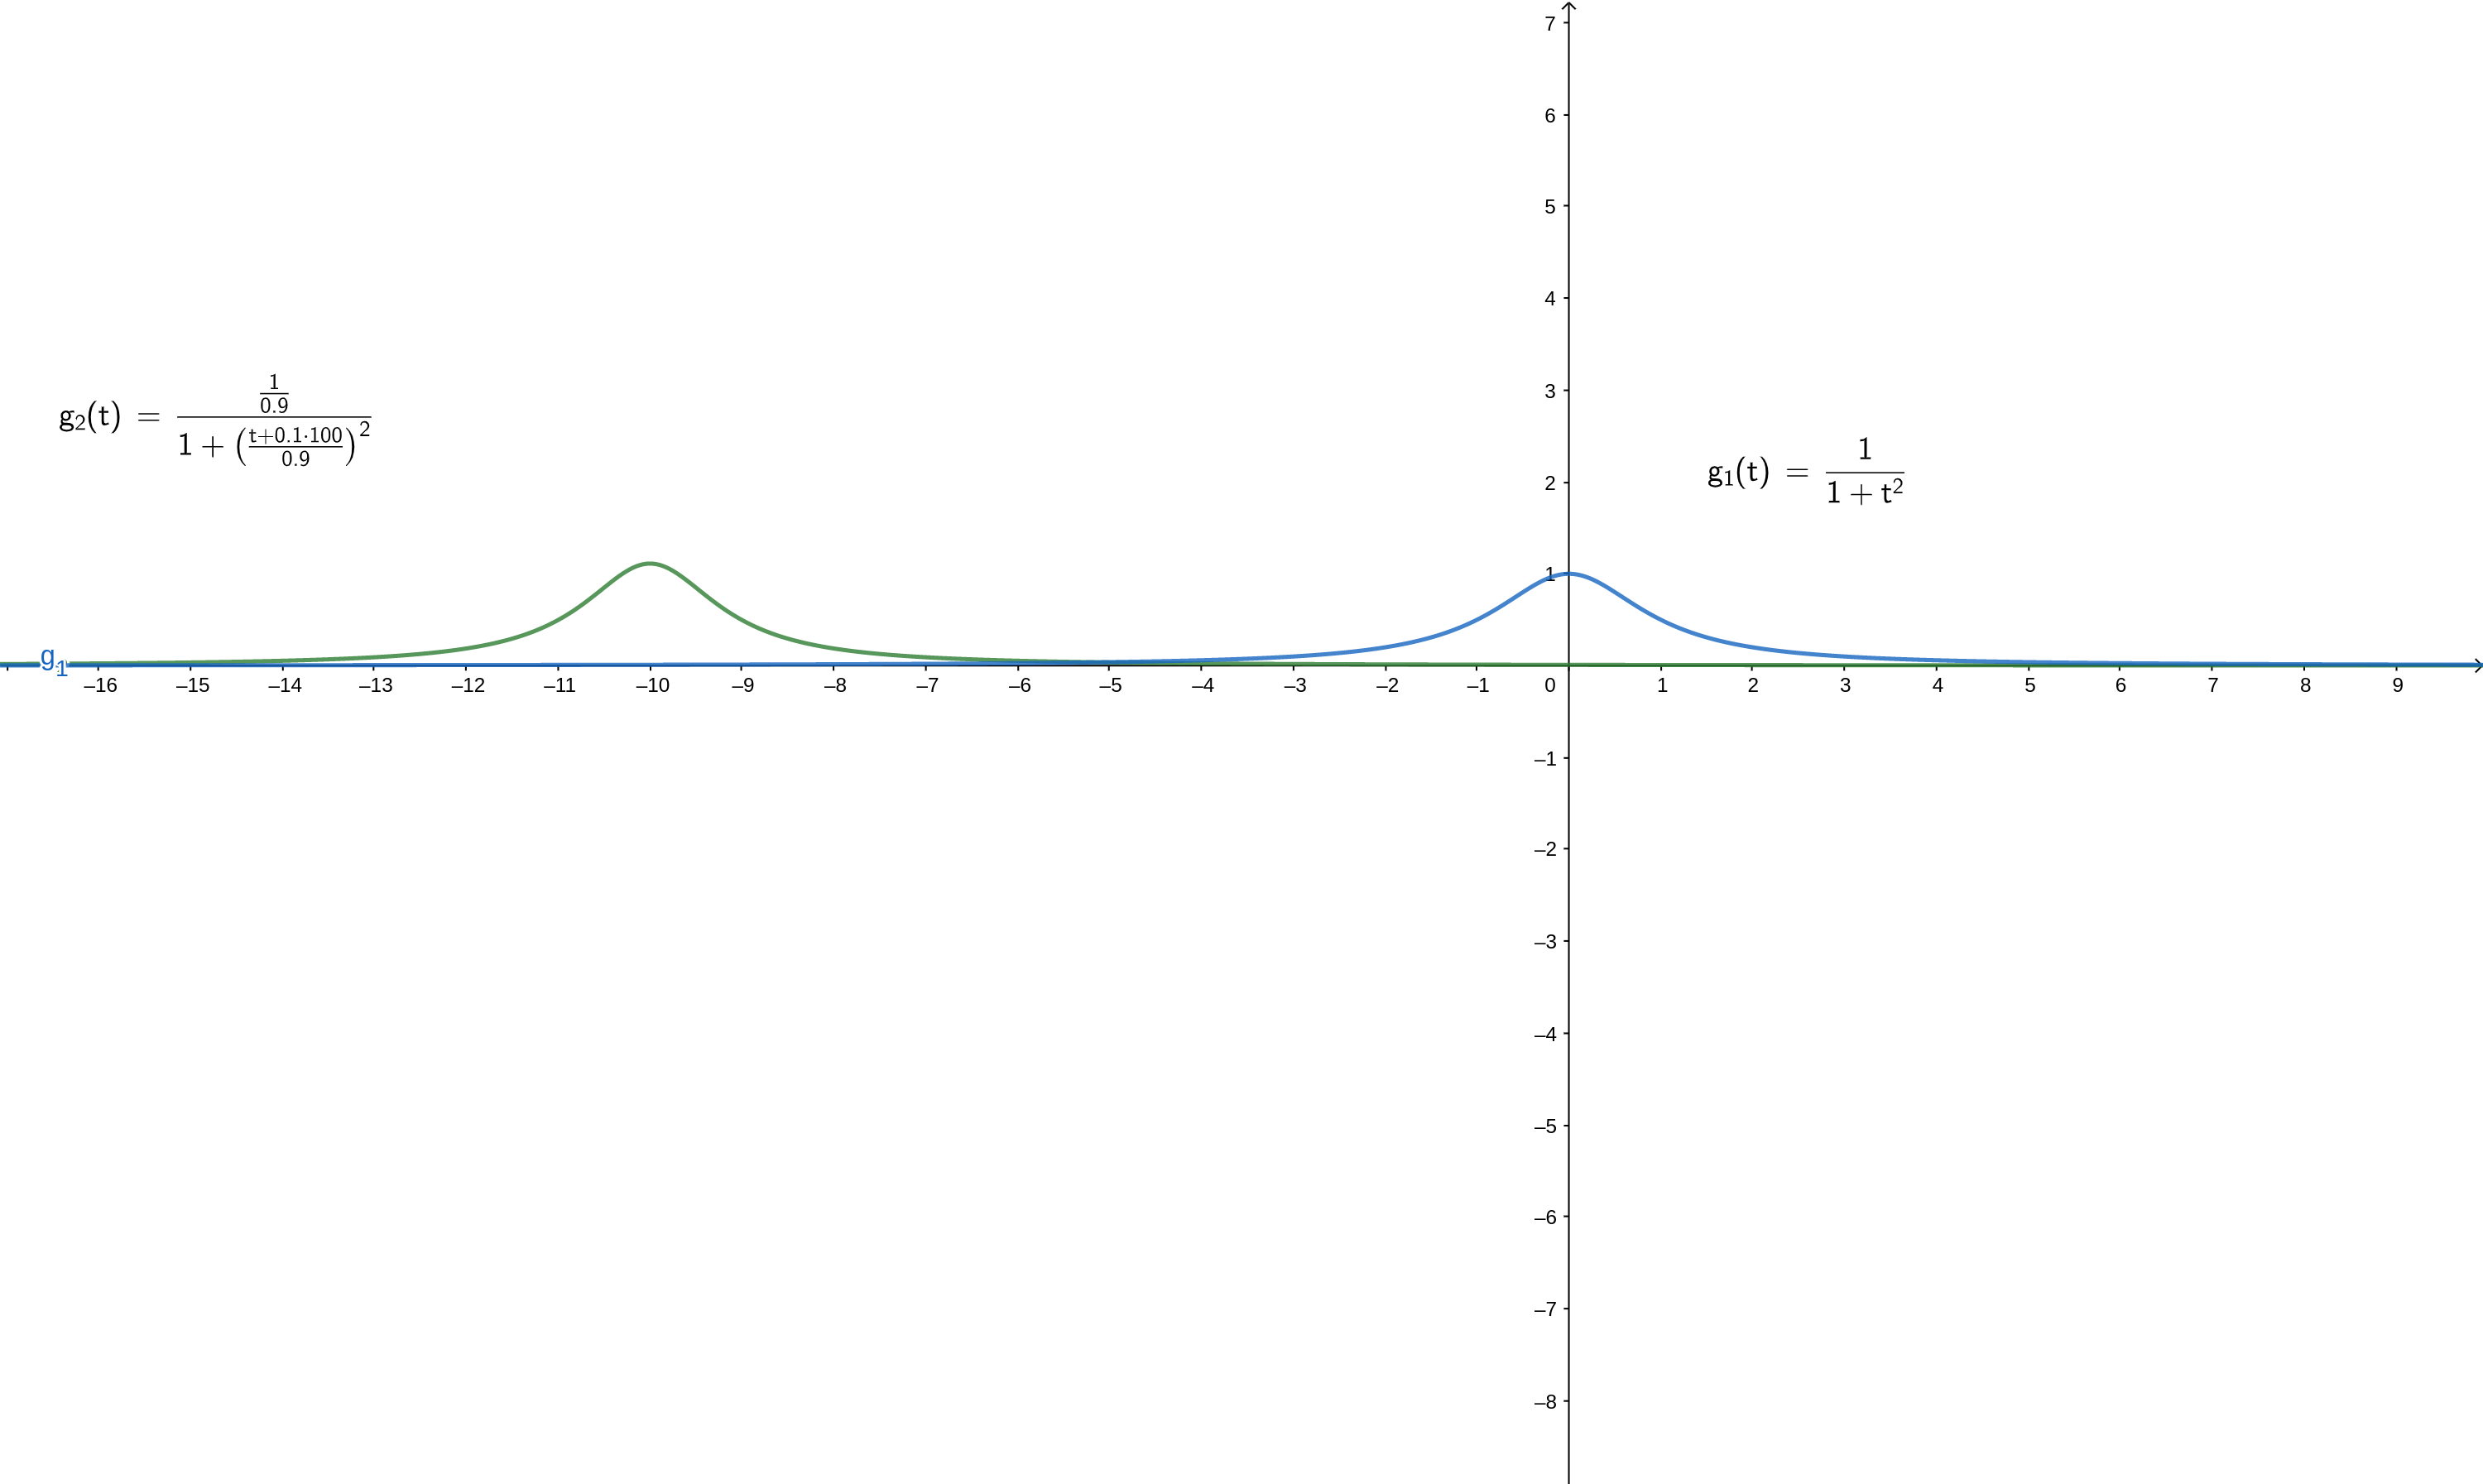
\includegraphics[width=1.0\textwidth]{img/geogebra-export_contraejemplo_Fourier.png}
    \caption{Como podemos ver en la imagen, para los valores $\epsilon=0.1$, $\xi=100$ y $M=5$ ambas funciones tienen soporte casi disjunto de manera que la diferencia entre ellas en el intervalo $[-5,5]$ coincide prácticamente con $g_1(t)$.}
    \label{fig:Grafica_funciones}
  \end{figure}


 
\medskip

\noindent El razonamiento anterior no ha tenido en cuenta la hipótesis de que la función $f$ debe tener soporte compacto, pero se ha realizado de esta manera por simplicidad en las cuentas, aunque puede adaptarse a este caso también.

\medskip

\noindent Para tratar de arreglar el problema del módulo de la transformada de Fourier  reemplazaremos las ondas sinusoidales de la transformada de Fourier por funciones localizadas con un soporte mayor en altas frecuencias que tendrán un mejor rendimiento para nuestro propósito. Estas funciones se denominan \textbf{ondeletas}. 

\medskip

\subsection{Alternativa: Las ondeletas}

\noindent Las ondeletas son pequeñas ondas estables bajo la acción de deformaciones, a diferencia de las ondas sinusoidales de Fourier. Definiremos la transformada de ondeletas y veremos que calcula, mediante convoluciones con bases de ondeletas, coeficientes estables bajo la acción de difeomorfismos.

\medskip

\noindent Al contrario que las bases de Fourier, las bases de ondeletas definen  representaciones dispersas de señales regulares a trozos, que podrían incluir transiciones y singularidades. En las imágenes, los mayores coeficientes de las ondeletas se localizan en el entorno de las esquinas y en las texturas irregulares.

\medskip

\noindent A modo de ejemplo vamos a ver la base de Haar que, aunque no sea la que utilicemos para construir nuestro propagador de dispersión, puede ayudar a entender mejor la filosofía de las ondeletas. Lo que sigue está basado en  \cite{MallatWavelets}.

\medskip

\noindent Se construye a partir de la siguiente función: 

$$ \psi(t)= \begin{cases} 
      1 & 0\leq t < 1/2 \\
      -1 & 1/2\leq t < 1 \\
      0 & \; \text{en otro caso},
   \end{cases}$$
\noindent podemos ver una representación gráfica en la \autoref{fig:Ondeleta_de_Haar}.
\begin{figure}[!h]
  \centering
  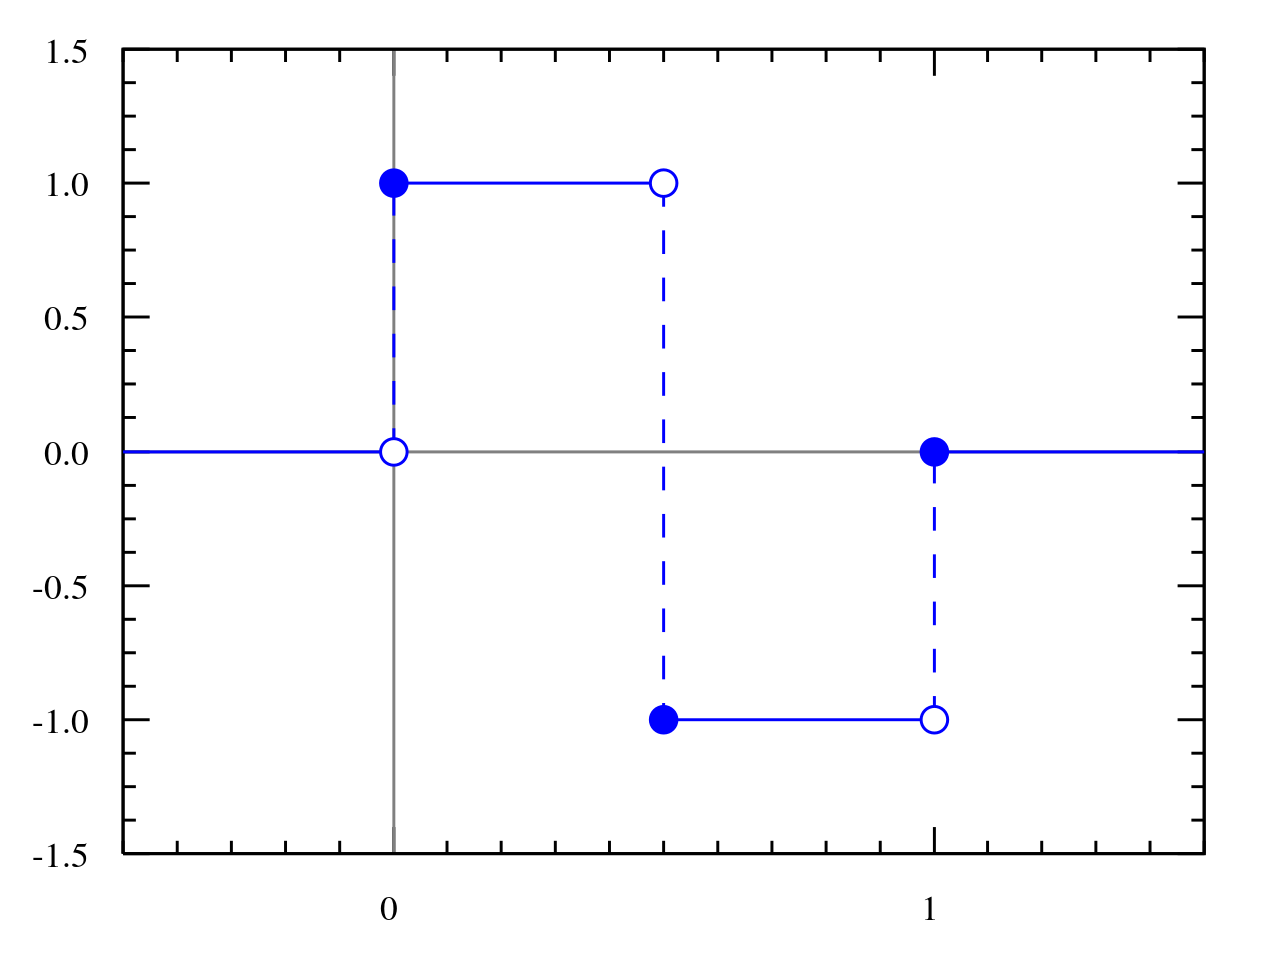
\includegraphics[width=0.5\textwidth]{img/Haar_wavelet.png}
  \caption{Representación gráfica de la ondeleta de Haar.}
  \label{fig:Ondeleta_de_Haar}
\end{figure}

\noindent A esta ondeleta la denominamos \textbf{ondeleta madre}, pues a partir de ella, podemos generar la siguiente base ortonormal

\medskip

$$\left \lbrace \psi_{j,n}(t)= \frac{1}{\sqrt{2^j}} \psi\left(\frac{t-2^jn}{2^j}\right) \right\rbrace_{(j,n) \in \mathbb{Z}^2}$$

\noindent del espacio $L^2(\mathbb{R})$ de señales con energía finita.

\noindent Así, cualquier señal $f$ de energía finita puede ser representada por los coeficientes que se obtienen mediante el producto interno en $L^2(\mathbb{R})$ con la base anterior: 

$$\langle f,\psi_{j,n} \rangle =\int_{-\infty}^{+\infty} f(t) \psi_{j,n} (t) dt  $$

\noindent y puede recuperarse sumando en su base ortonormal:

$$f=\sum_{j=-\infty}^{+\infty}\sum_{n=-\infty}^{+\infty}  \langle f,\psi_{j,n} \rangle \psi_{j,n} $$

\noindent Esto nos permite (igual que pasaba con el módulo de la Transformada de Fourier) trabajar en un dominio más sencillo donde procesar la información con mayor rapidez y posteriormente reconstruir la señal a partir de los coeficientes sin perder información. Algunas propiedades de la base de Haar son: 

\newpage

\begin{itemize}
  \item Cada ondeleta $\psi_{j,n}$ tiene media $0$ en su soporte $[2^jn, 2^j(n+1)]$.
  \item Si $f$ es localmente regular y el intervalo donde tiene soporte la ondeleta correspondiente es muy pequeño, debido a las propiedades de $f$, la función en el intervalo  $[2^jn, 2^j(n+1)]$ será prácticamente constante, lo que se traduce en que su coeficiente de ondeleta $\langle f,\psi_{j,n} \rangle$ es prácticamente cero.
  \item Los mayores coeficientes se localizan en los cambios bruscos de intensidad de señal, como pueden ser los bordes, las esquinas o las texturas en las imágenes, pues en estos casos somos capaces de encontrar un elemento de la base de Haar con cuyo soporte esté en el intervalo dónde se produzca el cambio de intensidad, y por lo tanto que tenga un coeficiente de ondeletas distinto de cero.
\end{itemize}

\noindent Para el caso concreto de imágenes (ver sección 1.1 de \cite{MallatWavelets}), las bases de ondeletas ortonormales pueden construirse a partir de bases ortonormales en señales de una dimensión. Lo haremos a partir de tres ondeletas para capturar las variaciones horizontales, verticales y diagonales presentes en la imagen. Así, denominamos a las ondeletas usadas como $\psi^1(x)$, $\psi^2(x)$ y $\psi^3(x)$ con $x=(x_1,x_2)\in \mathbb{R}^2$, dilatadas por el factor $2^j$ y trasladadas por $2^jn$ con $n=(n_1,n_2) \in \mathbb{Z}^2$, se construye una base ortonormal para el espacio $L^2(\mathbb{R}^2)$: 
$$\left \lbrace \psi_{j,n}^k(x)= \frac{1}{\sqrt{2^j}} \psi^k\left(\frac{x-2^jn}{2^j}\right) \right \rbrace_{(j,n) \in \mathbb{Z}^2}$$

\medskip

\noindent El soporte de la ondeleta $\psi_{j,n}^k(x)$ es un cuadrado proporcional a la escala $2^j$ como podemos ver en la \autoref{fig:base_haar}. Las bases de ondeletas en dos dimensiones se discretizan para definir bases ortonormales de imágenes de N píxeles.


\begin{figure} [!h]
  \centering
  
\includegraphics[width=0.8\textwidth]{img/base_haar_2d.png}
  \caption{En el ejemplo $1)$ podemos ver un ejemplo de filtro generado por el soporte de una ondeleta para la detección de líneas bordes verticales, en la imagen $2)$ podemos ver un ejemplo de filtro generado por el soporte de una ondeleta para la detección de bordes horizontales, y en el ejemplo $3)$ para las diagonales. Todas tienen soporte cuadrado.}
  \label{fig:base_haar}
\end{figure}

\noindent Igual que en el caso unidimensional, los coeficientes de ondeletas $\langle f,\psi_{j,n}^k \rangle$ serán pequeños si $f(x)$ es regular, y serán grandes cerca de los cambios bruscos de frecuencias como en los bordes o esquinas de las imágenes, como podemos ver en \autoref{fig:ejemplo_haar}.

\begin{figure} [!h]
  \centering
  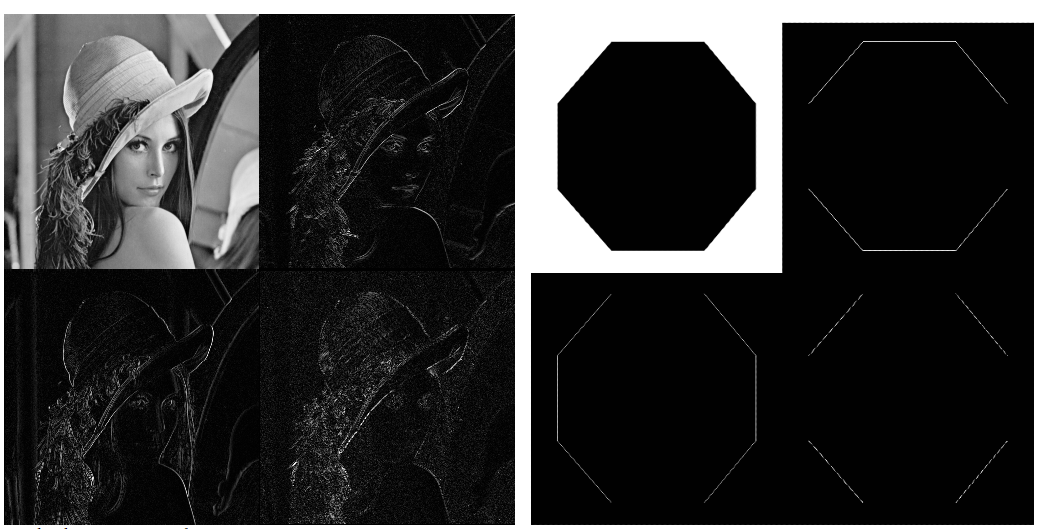
\includegraphics[width=0.8\textwidth]{img/ejemplos_haar_basis.png}
  \caption{Ejemplos de aplicar la base de Haar a dos imágenes. Los filtros resaltan los bordes en tres direcciones, horizontal (derecha) vertical (abajo) y en diagonal (abajo derecha). Imagen extraída de \cite{HaarBasis}.}
  \label{fig:ejemplo_haar}
\end{figure}

\medskip 

\noindent Volviendo al propósito de definir el propagador de dispersión, la ondeleta madre que elijamos y la base ortogonal que forme se verán afectadas normalmente por escalados y rotaciones, por lo tanto definimos: 

\begin{definicion}
  Una ondeleta madre escalada por un factor $2^{j}$ con $j \in \mathbb{Z}$ y rotada por $r \in G$ siendo $G$ el grupo finito de rotaciones, se escribe: 

  $$\psi_{2^j r}(x)=2^{j} \psi(2^j r^{-1} x).$$
\end{definicion}


\medskip

\noindent Su transformada de Fourier es $\widehat{\psi_{2^j r}}(\omega)=\widehat{\psi}(2^{-j} r^{-1} \omega)$.

\medskip

\noindent La transformada de dispersión que usaremos tendrá una base de ondeletas generada por una ondeleta madre del tipo:

$$\psi(x)=e^{i\eta x} \Theta(x)$$

\noindent donde $\Theta(x)$ es una función real con soporte en una bola de baja frecuencia en $x=0$, cuyo radio es del orden de $\pi$.

\medskip

\noindent Y como podemos ver:

\begin{equation}
  \widehat{\psi}(\omega)=\int_{\mathbb{R}^d}e^{i \eta x} \Theta(x) e^{-i\omega x} dx=\int_{\mathbb{R}^d}\Theta(x) e^{ix(\omega-\eta)} dx=\widehat{\Theta}(\omega-\eta).
\end{equation}

\medskip

\noindent Por lo tanto, $\widehat{\psi}(\omega)$ es real y con soporte en una bola de mismo radio pero centrada en $\omega=\eta$, que tras el escalado y rotación, queda: 
$$\widehat{\psi}_\lambda(\omega)= \widehat{\Theta} (\lambda^{-1}\omega-\eta),$$ 

\noindent donde $\lambda=2^jr \in 2^{\mathbb{Z}}\times G$. 

\noindent Por lo tanto $\widehat{\psi}_\lambda(\omega)$ tiene soporte en una bola centrada en $\lambda^{-1}\eta$ con radio proporcional a $|\lambda|=2^j$.
 
\medskip 

\subsection{La Transformada de Littlewood-Paley} \label{ch:seccion12}

\noindent Una vez conocemos, un poco más en profundidad, las ondeletas y su funcionamiento, pasamos a presentar la \textbf{Transformada de ondeleta de Littlewood-Paley}, que es la que emplearemos para construir el propagador de dispersión. Su expresión es la siguiente: 

\begin{equation}
  \forall x \in  \mathbb{R}^d \;\; W[\lambda]f(x)= f \ast \psi_\lambda(x)=\int f(u)\psi_\lambda(x-u) du .
\end{equation}

\noindent Donde $\ast$ denota la operación de convolución. 

\medskip

\noindent Calculamos su transformada de Fourier, para ello tendremos en cuenta el teorema de Convolución de la Transformada de Fourier: 

\begin{teorema} \label{Teorema::Convolucion}
 Sean $f$ y $g$ dos funciones integrables. Si 

 $$h(x)=(f\ast g)(x)=\int f(y)g(x-y) dy$$

 entonces: 

 $$\widehat{h}(\omega)=\widehat{f}(\omega) \widehat{g}(\omega)$$

 y 

 $$h(x)=(f \ast g)(x)= \int \widehat{f}(\omega) \widehat{g}(\omega) e^{-i\omega x} d\omega.$$
 
\end{teorema}

De esta manera, se tiene que: 

$$\widehat{W[\lambda]f}(\omega)=\widehat{f}(\omega)\widehat{\psi_\lambda}(\omega)=\widehat{f}(\omega)\widehat{\psi}(\lambda^{-1}\omega).$$

\noindent Además, teniendo en cuenta la propiedad que nos dice que si la función $f$ es real entonces su transformada coincide con el conjugado complejo $\widehat{f}(-\omega)=\overline{\widehat{f}(\omega)}$, podemos ver que: 

\begin{itemize}
  \item si $\widehat{\psi}(\omega)$ y $f$ son reales entonces $W[-\lambda]f= \overline{W[\lambda]f}$, utilizando la misma propiedad de antes. Además, si denotamos por $G^{+}$ al cociente de G sobre $\lbrace-\mathbb{1},\mathbb{1}\rbrace$, conjunto en el cual las dos rotaciones $r$ y $-r$ son equivalentes, sería suficiente calcular $W[2^jr]f$ para las rotaciones "positivas" de $G^{+}$.
  \item En cambio, si $f$ fuese compleja, entonces $W[2^jr]f$ tendría que calcularse para todo $r \in G$.
\end{itemize}

\medskip
 
\noindent Podemos entender, que cuanto menor sea el factor de escala que afecta a la ondeleta, más \entrecomillado{comprimida} estará esta, y viceversa. Por lo tanto podemos establecer una relación entre la frecuencia y la escala: 

\begin{itemize}
  \item A menor escala, más comprimida estará la ondeleta, los cambios en la señal se detectarán más rápidamente y las frecuencias obtenidas serán mayores. Véase la \autoref{fig:small_long_scale}.
  \item A mayor escala, la ondeleta estará más dilatada, los cambios se detectan en menor medida (solo si son lo suficientemente bruscos) y las frecuencias obtenidas serán menores.
\end{itemize}

\begin{figure} [!h]
  \centering
  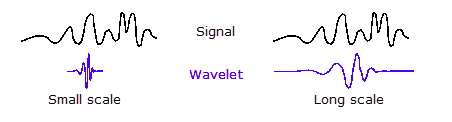
\includegraphics[width=0.8\textwidth]{img/Relacion_escala_frecuencia.png}
  \caption{Como podemos ver, en el caso de la izquierda la ondeleta (en color morado) se ve afectada por una menor escala, lo que le permitirá detectar con mayores frecuencias los cambios que se producen en la señal al convolucionar con esta a lo largo del tiempo. En cambio, en el segundo caso, se ve afectada por una escala mayor, lo que le impedirá detectar con tanta precisión los cambios que se produzcan en la señal. Imagen extraída de \cite{WAVELETS}.}
  \label{fig:small_long_scale}
\end{figure}

\medskip

\noindent Con la transformada de Littlewood-Paley ocurre lo mismo, a una cierta escala $2^J$ (con $J \in \mathbb{Z}$ fijo), solo retiene las ondeletas afectadas por un factor de escala $2^j > 2^{-J}$. Así, podemos obtener un umbral a partir del cual la base ortonormal de ondeletas no sería capaz de identificar cambios de frecuencias. Surge la necesidad, por tanto, de promediar las bajas frecuencias que no son cubiertas por estas ondeletas en un dominio proporcional al factor $2^J$:

\begin{equation}
  A_Jf=f \ast \phi_ {2^J} \; \; \text{con} \quad \; \phi_ {2^J}(x)=2^{-J} \phi(2^{-J}x).
\end{equation}

\medskip

\noindent Donde $\phi$ es una función fija, de la que dependerá la transformada de ondeleta.

\medskip

\noindent Así, si $f$ fuese real, entonces la transformada de ondeleta tendría la siguiente expresión: 

$$W_J f=\lbrace A_Jf,(W[\lambda]f)_{\lambda \in \Lambda_J} \rbrace$$ 

\noindent Es decir, estaría formada por el promedio de todas las odeletas de la base que no tienen soporte a la escala fijada $2^J$, y el conjunto de coeficientes producidos al convolucionar cada elemento de la base con $2^j>2^{-J}$ con la señal $f$. Para denotar esto indexamos por $\Lambda_J=\lbrace \lambda=2^jr:\;r\in G^{+}, \; 2^j>2^{-J}\rbrace$. 

\medskip

\noindent Su norma sería: 

\begin{equation} \label{eq::norma}
  \|W_Jf\|^2=\|A_Jf\|^2+\sum_{\lambda \in \Lambda_J} \|W[\lambda]f\|^2.
\end{equation}

\medskip
 
\noindent Si $J=\infty$ entonces todas las ondeletas de la base obtendrían coeficientes no nulos y por lo tanto 
$$W_\infty f=\lbrace W[\lambda]f\rbrace_{\lambda \in \Lambda_\infty},$$ 

\noindent con $\Lambda_\infty=2^\mathbb{Z} \times G^{+}$. 

\noindent Su norma en este caso sería 

$$\|W_\infty f\|^2=\sum_{\lambda \in \Lambda_\infty} \|W[\lambda]f\|^2.$$

\noindent En el caso en que $f$ sea compleja, se incluyen todas las rotaciones y obtnemos $W_Jf=\lbrace A_J f,(W[\lambda]f)_{-\lambda,\lambda \in \Lambda_J} \rbrace$ y $W_\infty f=\lbrace W[\lambda]f\rbrace_{-\lambda,\lambda \in \Lambda_\infty}$. 

\medskip

\noindent La siguiente proposición da una condición estándar de Littlewood-Paley para que $W_J$ sea unitario.

\begin{proposicion} \label{unitario}
 Para cualquier $J \in \mathbb{Z}$ o $J=\infty$, $W_J$ es unitario en el espacio de funciones reales o complejas de $L^2(\mathbb{R}^d)$ si y solo si para casi todo $\omega \in \mathbb{R}^d$ se cumple: 
    \begin{equation}\label{eq::1.2}
        \beta \sum_{j=-\infty}^\infty \sum_{r \in G} |\widehat{\psi}(2^{-j}r^{-1}\omega)|^2=1 \; \; y
        \;\;|\widehat{\phi}(\omega)|^2= \beta \sum_{j=-\infty}^0 \sum_{r\in G} |\widehat{\psi}(2^{-j}r^{-1}\omega)|^2,
    \end{equation}
 donde $\beta=1$ para funciones complejas y $\beta=\frac{1}{2}$ para funciones reales.
\end{proposicion}

\begin{proof}
\noindent Si $f$ es una función compleja, tenemos que $\beta=1$ y vamos a demostrar que \eqref{eq::1.2} es equivalente a : 

\begin{equation} \label{eq::1.3}
  \forall J \in \mathbb{Z} \; \; \; \left|\widehat{\phi}\left(2^J\omega\right)\right|^2 + \sum_{j>-J,r\in G}\left|\widehat{\psi}\left(2^{-j}r^{-1}\omega\right)\right|^2=1.
\end{equation}

\noindent Para ello, partimos de que si sustituimos $\beta=1$ en \eqref{eq::1.2} se tiene que: 
     \begin{align*}
        \sum_{j=-\infty}^\infty \sum_{r \in G} |\widehat{\psi}(2^{-j}r^{-1}\omega)|^2=1 & \; \; y
        \;\;|\widehat{\phi}(\omega)|^2= \sum_{j=-\infty}^0 \sum_{r\in G} |\widehat{\psi}(2^{-j}r^{-1}\omega)|^2.
    \end{align*}

\noindent Si ahora sumamos $\sum_{j=0}^{\infty} \sum_{r\in G} |\widehat{\psi}(2^{-j}r^{-1}\omega)|^2$ en el segundo término obtenemos: 

$$|\widehat{\phi}(\omega)|^2 + \sum_{j=0}^{\infty} \sum_{r\in G} |\widehat{\psi}(2^{-j}r^{-1}\omega)|^2=1.$$

\noindent Por otro lado si vamos a la expresión a la que queremos llegar se tiene que: 

\begin{align*}
  &\forall J \in \mathbb{Z} \; \; \; \left|\widehat{\phi}\left(2^J\omega\right)\right|^2 + \sum_{j>-J,r\in G}\left|\widehat{\psi}\left(2^{-j}r^{-1}\omega\right)\right|^2=1 \iff \\
  &\iff \forall J \in \mathbb{Z} \; \; \; \left|\widehat{\phi}\left(2^J\omega\right)\right|^2=\sum_{j=-\infty}^{-J} \sum_{r\in G} |\widehat{\psi}(2^{-j}r^{-1}\omega)|^2.
\end{align*}

\noindent Con lo que si demostramos esto último tendríamos que \eqref{eq::1.2} y \eqref{eq::1.3} son equivalentes para el caso $\beta=1$. 


     \begin{align*}
        \left|\widehat{\phi}\left(2^J\omega\right)\right|^2 & =\sum_{j=-\infty}^{0} \sum_{r\in G} |\widehat{\psi}(2^{-j}r^{-1}2^J\omega)|^2 \\
        & = \sum_{j=-\infty}^{0} \sum_{r\in G} |\widehat{\psi}(2^{J-j}r^{-1}\omega)|^2  \\
        & =\sum_{j=-\infty}^{-J} \sum_{r\in G} |\widehat{\psi}(2^{-j}r^{-1}\omega)|^2  
    \end{align*}
    
\noindent con lo que queda demostrado que \eqref{eq::1.2} y \eqref{eq::1.3} son equivalentes. Teniendo en cuenta que $\widehat{W\left[2^jr\right]f}(\omega)=\widehat{f}(\omega)\widehat{\psi}_{s^jr}(\omega)$, multiplicando \eqref{eq::1.3} por $|\widehat{f}(\omega)|^2$ obtenemos: 

$$\forall J \in \mathbb{Z} \; \; \; \left|\widehat{\phi}\left(2^J\omega\right)\right|^2 \left|\widehat{f}(\omega)\right|^2 + \sum_{j>-J,r\in G}\left|\widehat{f}(\omega)\right|^2\left|\widehat{\psi}\left(2^{-j}r^{-1}\omega\right)\right|^2=\left|\widehat{f}(\omega)\right|^2.$$

\noindent Si ahora integramos en ambos miembros en $\mathbb{R}^d$ obtenemos: 

     \begin{align*}
        \int_{\mathbb{R}^d}\left(\left|\widehat{\phi}\left(2^J\omega\right)\right|^2 \left|\widehat{f}(\omega)\right|^2 + \sum_{j>-J,r\in G}\left|\widehat{f}(\omega)\right|^2\left|\widehat{\psi}\left(2^{-j}r^{-1}\omega\right)\right|^2 \right) d\omega=\int_{\mathbb{R}^d}\left|\widehat{f}(\omega)\right|^2 d\omega.
    \end{align*}

\noindent Si le aplicamos la identidad de Plancharel \eqref{eq::Plancharel} se obtiene:

$$\int_{\mathbb{R}^d}\left(\left|\phi\left(2^J\omega\right)\right|^2 \left|f(\omega)\right|^2 + \sum_{j>-J,r\in G}\left|f(\omega)\right|^2\left|\psi\left(2^{-j}r^{-1}\omega\right)\right|^2 \right) d\omega=\int_{\mathbb{R}^d}\left|f(\omega)\right|^2 d\omega.$$

\noindent Si ahora recordamos la expresión \eqref{eq::norma}, tenemos que la expresión anterior equivale a:

$$\|A_Jf\|^2+\sum_{\lambda \in \Lambda_j} \|W[\lambda]f\|^2=\|W_J f\|^2=\|f\|^2,$$

\noindent que es válido para todo $J$ y en particular también cuando $J=\infty$.

\medskip

\noindent Recíprocamente, si tenemos que $\|W_J f\|^2=\|f\|^2$ entonces \eqref{eq::1.3} se verifica para casi todo $\omega$. De no ser así podríamos contruir una función $f$ no nula cuya transformada de fourier $\widehat{f}$ tuviera soporte en el dominio de $\omega$ donde \eqref{eq::1.3} no fuera válido, y en estos casos al aplicar la fórmula de Plancherel se verificaría que $\|W_J f\|^2 \neq \|f\|^2$ contradiciendo la hipótesis. Y como la expresión \eqref{eq::1.3} era equivalente a la que nos daba el teorema tenemos demostrado el resultado para el caso en que $f$ sea compleja. 

\medskip

\noindent Si ahora $f$ es real entonces $|\widehat{f}(\omega)|=|\widehat{f}(-\omega)|$ lo que implica que $\|W[2^jr]f\|=\|W[-2^jr]f\|$. Por lo que $\|W_J f\|$ permanece constante si restringimos $r$ a $G^+$ y multiplicando $\psi$ por $\sqrt{2}$ se obtiene la condición \eqref{eq::1.2} con $\beta=\frac{1}{2}$. \qedhere

\end{proof}

\medskip


\subsection{Convenios para futuras secciones}

\noindent Llegados a este punto, ya tenemos la transformada de ondeletas que vamos a utilizar para la construcción del PD, ahora vamos a establecer algunas características que impondremos a los distintos elementos que la componen y que usaremos de ahora en adelante: 

\begin{itemize}
    \item $\widehat{\psi}$ es una función real que satisface la condición \eqref{eq::1.2}. Lo que implica que $\widehat{\psi}(0)=\int \psi(x)dx=0$ y $|\widehat{\phi}(r\omega)|=|\widehat{\phi}(\omega)| \;\; \forall r\in G$.
    \item $\widehat{\phi}(\omega)$ es real y simétrica, por lo que $\phi$ también lo será y $\phi(rx)=\phi(x) \;\; \forall r \in G$. 
    \item Las derivadas de $\phi$ pertenecen a $L^1(\mathbb{R}^d)$.
\end{itemize}

\medskip

\noindent A continuación introducimos algo de notación que emplearemos de ahora en adelante: 

\begin{itemize}

  \item Se denota $g \circ f(x)=f(gx)$ a la acción de un elemento del grupo $g\in G$.
  \item Un operador  $\mathcal{R}$ parametrizado por $p$ es denotado por $\mathcal{R}[p]$ y $\mathcal{R}[\Omega]=\lbrace \mathcal{R}[p] \rbrace_{p \in \Omega}$. 
\end{itemize}

\noindent Un cambio de variable en la integral de la transformada de ondeleta nos muestra que si $f$ se escala y rota, $2^lg \circ f=f(2^lgx)$ con $2^lg \in 2^{\mathbb{Z}} \times G$, entonces la transformada de ondeleta se escala y rota de acuerdo a: 

\begin{equation}
  W[\lambda](2^lg\circ f)=2^lg \circ W[2^{-l}g\lambda]f.
\end{equation}

\medskip

\noindent Como $\phi$ es invariante a rotaciones en $G$, podemos comprobar que $A_J$ conmuta con las rotaciones de $G$: $A_J(g\circ f)=g\circ A_J f \;\; \forall g \in G$. 

\section{El operador de dispersión sobre un camino ordenado}

%Esto debería intentar explicarlo mejor?
\noindent La transformada de Littlewood-Paley definida anteriormente es Lipschitz-continua bajo la acción de difeomorfismos porque las ondeletas son funciones regulares y localizadas. Sin embargo, todavía no es invariante a traslaciones y $W[\lambda]f=f\ast\psi_\lambda$ se traslada cuando lo hace $f$. Así, nuestro próximo objetivo será conseguir calcular coeficientes que sean invariantes a traslaciones, que permanezcan estables bajo la acción de difeomorfismos y que retengan la información en altas frecuencias que proporcionan las ondeletas, reuniendo todas estas características tendríamos el operador que necesitamos para la construcción del PD. 

\medskip 

\noindent Los coeficientes invariantes por traslaciones los obtendremos gracias a la acción de un operador no lineal aplicando el siguiente lema: 

%No se si perder tiempo en buscar la dem
\begin{lema} \label{lema:Invarianza_traslaciones_integral}
  Si $U[\lambda]$ es un operador definido en $L^2(\mathbb{R}^d)$, no necesariamente lineal pero que conmuta con traslaciones, entonces $\int_{\mathbb{R}^d} U[\lambda]f(x)dx$ es invariante a traslaciones si es finito.
\end{lema}

\begin{proof}
  Sea $f \in L^2(\mathbb{R}^d)$, $c \in \mathbb{R}^d$ y $L_cf(x)=f(x-c)$ una traslación de $f$, como $U[\lambda]f$ conmuta con traslaciones se tiene que: 
  \begin{align*}
    U[\lambda]L_cf(x)&=U(f(x-c)) \\
    &=U(f)(x-c) \\
    &=L_cU[\lambda]f(x)\\
  \end{align*}

  \noindent Vamos a comprobar ahora que si $\int_{\mathbb{R}^d} U[\lambda]f(x)dx$ es finito, entonces la integral es invariante a traslaciones. En otras palabras, queremos comprobar que : 

  $$\int_{\mathbb{R}^d} U[\lambda]L_cf(x)dx=\int_{\mathbb{R}^d} U[\lambda]f(x)dx$$

  Para ello, si tenemos en cuenta la conmutatividad del operador $U[\lambda]$ se tiene que 
  
  \begin{align*}
    \int_{\mathbb{R}^d} U[\lambda]L_cf(x)dx &= \int_{\mathbb{R}^d} U[\lambda](f(x-c))dx \\
    &= \int_{\mathbb{R}^d} U[\lambda](f)(x-c)dx. \\
  \end{align*}

  \noindent Y tras esto basta tener en cuenta el cambio de variable $y=x-c$ que tiene Jacobiano $J=1$ y se tendría que en la expresión anterior
  \begin{align*}
    \int_{\mathbb{R}^d} U[\lambda](f)(x-c)dx = \int_{\mathbb{R}^d} U[\lambda](f)(y)dy .\\
  \end{align*}
  
  \noindent Por lo que la integral es invariante por traslaciones.
\end{proof}

\noindent En nuestro caso $W[\lambda]f=f\ast\psi_\lambda$ es un ejemplo trivial de este lema, pues se trata de un operador que conmuta con traslaciones y $\int_{\mathbb{R}^d} f \ast \psi(x) dx=0$ porque $\int_{\mathbb{R}^d} \psi(x)dx=0$.

\medskip

\noindent Esto nos enseña, que para obtener un operador invariante por traslaciones y no trivial $U[\lambda]f$, es necesario componer $W[\lambda]$ con un operador extra $M[\lambda]$ que sea no lineal, y que se conoce como \entrecomillado{demodulación}, que transforma $W[\lambda]f$ en una función de menor frecuencia con integral distinta de cero. Además, la elección de $M[\lambda]$ debe preservar la Lipschitz-continuidad bajo la acción de difeomorfismos.    
En resumen, queremos un operador no lineal que produzca coeficientes invariantes por traslaciones no triviales y que además conserve la Lipschitz-continuidad.


\medskip

\noindent Vamos a poner un ejemplo para entender mejor lo que se ha comentado anteriormente: 

\subsection{Ejemplo para obtener coeficientes invariantes por traslaciones}

\noindent Si la \textbf{ondeleta madre} fuese $\psi(x)=e^{i\eta x}\Theta(x)$, entonces los elementos de la base tendrían la forma $\psi_\lambda(x)=e^{i\lambda\eta x}\Theta_\lambda(x)$, y por lo tanto 


\begin{align} \label{eq::1.4}
  W[\lambda]f(x) &= f \ast \phi_\lambda (x) \\
  &= f \ast e^{i\lambda\eta x}\Theta_\lambda(x) \\
  &=e^{i\lambda\eta x}(e^{-i\lambda\eta x}f(x) \ast \Theta_\lambda(x)) \\
  &=e^{i\lambda\eta x}(f^\lambda \ast \Theta_\lambda(x)),\\
\end{align}

\noindent con $f^\lambda(x)=e^{-i\lambda\eta x}f(x)$.

\medskip

\noindent En este caso, se podría obtener un operador invariante por traslaciones si se cancela el término de modulación $e^{i\lambda\eta x}$ con una función $M[\lambda]$ pertinente. Por ejemplo: 

\begin{equation}
  M[\lambda]h(x)=e^{-i\lambda\eta x} e^{-i \Phi(\widehat{h}(\lambda\eta))}h(x).
\end{equation}

\noindent Dónde $\Phi(\widehat{h}(\lambda\eta))$ es la fase compleja de $\widehat{h}(\lambda\eta)$. Este registro de fase no lineal garantiza que $M[\lambda]$ conmuta con las traslaciones, ya que: 


\begin{align*}
  \int_{\mathbb{R}^d} M[\lambda]W[\lambda] f(x) dx &= \int_{\mathbb{R}^d} e^{-i\lambda \eta} e^{-i \Phi (\widehat{W[\lambda\eta]f})} \left( e^{i\lambda\eta x} \left( e^{-i\lambda\eta x} f \ast \Theta_\lambda (x)\right)\right) dx \\
  &= e^{-i \Phi (\widehat{f}(\lambda\eta)\widehat{\psi_\lambda}(\lambda\eta))} \int_{\mathbb{R}^d} e^{-i\lambda\eta x} f \ast \Theta_\lambda (x) dx \\
  &=e^{-i \Phi (\widehat{f}(\lambda\eta)\widehat{\psi_\lambda}(\lambda\eta))} \int_{\mathbb{R}^d}e^{-i\lambda\eta x} f(x) dx  \int_{\mathbb{R}^d}\Theta_\lambda (x) dx  \\
  &=e^{-i \Phi (\widehat{f}(\lambda\eta)\widehat{\psi_\lambda}(\lambda\eta))} \cdot \widehat{f}(\lambda\eta) \cdot  \widehat{\Theta_\lambda}(0)\\
  &=\left| \widehat{f}(\lambda\eta) \cdot  \widehat{\Theta_\lambda}(0) \right|^2 \\
  &=\left| \widehat{f}(\lambda\eta)\right|^2 \left| \widehat{\Theta_\lambda}(0) \right|^2  \\
  &=\left| \widehat{f}(\lambda\eta)\right|^2 \left| \widehat{\Theta}(0) \right|^2 
\end{align*}

\noindent que como podemos ver, la integral tiene un valor no trivial y por otra parte obtenemos el módulo de la transformada que como habíamos visto en el Lema \ref{lema::invarianza_traslaciones} era invariante por traslaciones. No obstante, no utilizaremos este operador para nuestro propósito pues además de ser complejo no verifica la invarianza bajo la acción de difeomorfismos.

\subsection{El operador módulo}

\noindent En nuestro caso, para preservar la Lipschitz-continuidad bajo la acción de difeomorfismos necesitamos que $M[\lambda]$ conmute con éstos y que además sea no expansiva para garantizar la estabilidad en $L^2(\mathbb{R}^d)$. Se puede comprobar que entonces $M[\lambda]$ tiene que ser necesariamente un operador punto a punto \cite{JBrunaOperatorsCommutingDiff}, lo que significa que el operador $M[\lambda]h(x)$ que buscamos dependería únicamente del valor de $h$ en el punto $x$.

\medskip

\noindent Para obtener mejores propiedades vamos a imponer también que $\|M[\lambda]h\|=\|h\| \; \; \forall h \in L^2(\mathbb{R}^d)$, lo que implica entonces que $|M[\lambda]h|=|h|$, ya que:  

\begin{align*}
  \|M[\lambda]h\|=\|h\| &\iff \left(\int_{\mathbb{R}^d} |M[\lambda]h (x)|^2 dx \right)^{\frac{1}{2}} =\left(\int_{\mathbb{R}^d} |h(x)|^2 dx \right)^{\frac{1}{2}} \\
  & \iff \int_{\mathbb{R}^d} |M[\lambda]h (x)|^2 dx=\int_{\mathbb{R}^d} |h(x)|^2 dx \\
  & \iff \int_{\mathbb{R}^d} |M[\lambda]h (x)|^2-|h(x)|^2 dx = 0 \\
  & \iff |M[\lambda]h (x)|^2 - |h(x)|^2 = 0 \\
  & \iff |M[\lambda]h (x)| = |h(x)|.
\end{align*}

\medskip

\noindent Para llegar a la conclusión que sugiere el autor \cite{GroupInvariantScattering}, se ha supuesto que $\left|M[\lambda]h(x) \right| \geq \left| h(x)\right| \;\; \forall x \in \mathbb{R}^d$, que junto con el hecho de que las dos funciones que se restan en el integrando son positivas, nos dan el resultado buscado.  

\medskip

\noindent Para satisfacer todas las restricciones, utilizaremos el operador $M[\lambda]h=|h|$, que además elimina todas las variaciones de fase \cite{bruna2013invariant}. Se obtiene entonces de \eqref{eq::1.4} que este módulo transforma $W[\lambda]f$ en una señal de menor frecuencia que la original:

$$M[\lambda]W[\lambda]f=|W[\lambda]f|=|f^\lambda \ast \Theta_\lambda|.$$

\noindent Vamos a visualizar con un ejemplo cómo, al interferir dos señales con este operador, la frecuencia resultante es menor que cada una de las originales. 

\medskip

\noindent Si 

$$f(x)=\cos(\xi_1 x)+a\cos(\xi_2 x)$$

\noindent donde $\xi_1 > 0$ y $\xi_2 > 0$ están en la banda de frecuencia cubierta por $\widehat{\psi}_\lambda$, entonces al aplicar el operador módulo obtenemos: 

$$|f \ast \psi_\lambda (x) |=2^{-1} |\widehat{\psi}_\lambda(\xi_1)+a\widehat{\psi}_\lambda(\xi_2)e^{i(\xi_2-\xi_1)x}|$$

\noindent que oscila entre la frecuencia de interferencias $|\xi_2-\xi_1|$, que como vemos es menor que $|\xi_1|$ y $|\xi_2|$.

\medskip

\noindent De esta manera, por la forma en que hemos construido el operador $U[\lambda] f$ la integración de $\int_{\mathbb{R}^d}U[\lambda]f(x) dx= \int_{\mathbb{R}^d} | f \ast \psi_\lambda(x)|dx$ es invariante por traslaciones, pero elimina todas las altas frecuencias de $|f \ast \psi_\lambda(x)|$. Para recuperarlas, el PD calcula los coeficientes de ondeletas para cada $U[\lambda]f$ que son $\lbrace U[\lambda]f \ast \psi_{\lambda'}\rbrace_{\lambda'}$. De nuevo, los coeficientes invariantes a traslaciones se obtienen con el módulo $U[\lambda']U[\lambda]f=|U[\lambda]f \ast \psi_{\lambda'}|$ y después integrando $\int_{\mathbb{R}^d} U[\lambda']U[\lambda]f(x) dx$. 

\medskip

\noindent Veamos esto con el mismo ejemplo de antes $f(x)=\cos(\xi_1 x)+a\cos(\xi_2 x)$ pero con $a<1$. Si $|\xi_2-\xi_1| << |\lambda|$ con $|\xi_2 - \xi_1|$ en el soporte de $\widehat{\psi}_{\lambda'}$, entonces $U[\lambda']U[\lambda]f$ es proporcional a $a\cdot |\psi_\lambda(\xi_1)|\cdot |\psi_{\lambda'}(|\xi_2-\xi_1|)|$. La segunda ondeleta $\widehat{\psi}_{\lambda'}$ captura las interferencias creadas por el módulo, entre la frecuencia de las componentes de $f$ y el soporte de $\widehat{\psi_\lambda}$.

\medskip

\subsection{Definición de camino de frecuencias y propiedades.}

\begin{definicion}
Una secuencia ordenada $p=(\lambda_1,\lambda_2, \ldots , \lambda_m)$ con $\lambda_k \in \Lambda_\infty=2^{\mathbb{Z}} \times G^{+} $ se denomina \textbf{camino}. Al camino vacío se le denota por $p=\emptyset$. 
\end{definicion}


\begin{definicion}
Un propagador de dispersión (PD) es un producto de operadores de la forma $U[\lambda]f=M[\lambda]W[\lambda]f=|f \ast \psi_\lambda|=\left | \int_{\mathbb{R}^d} f(u)\psi_\lambda(x-u) du \right|$ para $f \in L^2(\mathbb{R}^d)$ no conmuntativos por un camino ordenado:

\begin{equation}
  U[p]f=U[\lambda_m] \ldots U[\lambda_2]U[\lambda_1],
\end{equation}

con $U[\emptyset]=Id$
\end{definicion}

\noindent El operador $U[p]$ está bien definido en $L^2(\mathbb{R}^d)$ porque $\left|\left| U[\lambda]f \right|\right| = \|f\| \leq \|\psi_\lambda\|_1 \|f\|$ para todo $\lambda \in \Lambda_\infty$. 

\noindent El PD es por tanto una cascada de convoluciones y módulos: 

\begin{equation}
  \left| |f \ast \psi_{\lambda_1} | \ast \psi_{\lambda_2} | \ldots | \ast \psi_{\lambda_m} \right|  
\end{equation}

\medskip

\noindent Cada $U[\lambda]$ filtra la frecuencia del componente en la banda cubierta por $\widehat{\psi}_\lambda$ y lo aplica en un espacio de frecuencias menores con la operación módulo.

\noindent A continuación vamos a probar ciertas propiedades que tienen los caminos de frecuencias tal y como los hemos descrito anteriormente. Para ello empezamos con algunas definiciones que serán de utilidad:

\begin{definicion}
Escribimos la rotación y reescalado de un camino $p$ mediante $2^lg \in 2^\mathbb{Z}\times G$ como $2^lgp=(2^lg\lambda_1,2^lg\lambda_2,\ldots,2^lg\lambda_m)$.
\end{definicion}

\begin{definicion}
La concatenación de dos caminos $p$ y $p'$ se denota por $$p+p'=(\lambda_1,\lambda_2,\ldots,\lambda_m,\lambda_1',\lambda_2',\ldots,\lambda_{m'}').$$

\noindent En el caso particular de $p+\lambda=(\lambda_1,\lambda_2,\ldots,\lambda_m,\lambda)$
\end{definicion}

\noindent Con esta notación: 

\begin{proposicion} \label{proposicionSumaCaminos}
Sean $p, p'$ dos caminos, se tiene que :
$$U[p+p']=U[p']U[p]$$
\end{proposicion}

\begin{proof}
Como $p+p'=(\lambda_1,\lambda_2,...,\lambda_m,\lambda_1',\lambda_2',...,\lambda_{m'}')$ entonces siguiendo la definición de $U[p]$ se tiene que: 

\begin{equation}
  U[p+p']=U[\lambda'_{m'}]\ldots U[\lambda'_2]U[\lambda'_1]U[\lambda_{m}]\ldots U[\lambda_2]U[\lambda_1]=U[p']U[p] 
\end{equation}
\end{proof}

\medskip

\noindent En la \autoref{ch:seccion12} veíamos que si $f$ era compleja, entonces su transformada de ondeletas era $ W_\infty=\lbrace W[\lambda]f \rbrace_{\lambda , -\lambda  \in \Lambda_{\infty} }$. Pero en este caso, gracias al módulo, tras la iteración $U[\lambda_1]f=\left|W[\lambda_1]f\right|$ sería una función real. Por tanto, las siguientes transfomadas de ondeletas solo haría falta calcularlas para $\lambda_k \in \Lambda_\infty$. Por eso, los propagadores de dispersión de funciones complejas se definen sobre caminos \entrecomillado{positivos} $p=(\lambda_1,\lambda_2, \ldots , \lambda_m)$ y caminos \entrecomillado{negativos} $-p=(-\lambda_1,\lambda_2, \ldots , \lambda_m)$.

\medskip

\noindent Sin embargo, para simplificar cálculos, todos los resultados siguientes se haran sobre PD aplicados a funciones reales.

\subsection{Construcción del operador de dispersión.}

\noindent En este momento, disponemos de un operador $U[\lambda]$ que cumple todas las condiciones deseables, por lo que en esta sección vamos a ser capaces de llegar finalmente a la modelización matemática de una CNN.

\begin{definicion} \label{def:S_barra}
Sea $\mathcal{P}_\infty$ el conjunto de todos los caminos finitos. La transformada de dispersión de $f \in L^1(\mathbb{R}^d)$ se define para cualquier camino $p \in \mathcal{P}_\infty$ como:

\begin{equation}
  \overline{S}f(p)=\int_{\mathbb{R}^d}U[p]f(x)dx 
\end{equation}

\end{definicion}

\medskip

\noindent El operador $\overline{S}f(p)$ es invariante a traslaciones de $f$, pues el operador $U[p]$ hemos visto que cumple las propiedades necesarias para que el valor de la integral sea finito y por lo tanto sea invariante por traslaciones, y transforma $f \in L^1(\mathbb{R}^d)$ en una función en el camino de frecuencias variable $p$.

\medskip

\noindent Esta defnición, guarda muchas similitudes con la el módulo de la transformada de Fourier. Pero en este caso, la transformada es Lipschitz-continua bajo la acción de difeomorfismos, porque se calcula iterando en transformadas de ondeletas y módulos que, como hemos visto anteriormente, son estables. 

\medskip

\noindent No obstante, para problemas de clasificación, es mucho más frecuente calcular pequeños descriptores que sean invariantes por traslaciones frente a una escala predefinida $2^J$, manteniendo las frecuencias superiores a $2^{-J}$, lo que nos permite ver esta variabilidad espacial. Esto se consigue convolucionando la transformada con una ventana escalada a la frecuencia deseada, en nuestro caso $\phi_{2^J}(x)=2^{-J}\phi(2^{-J}x)$. 

\begin{definicion}
Sea $J \in \mathbb{Z}$ y $\mathcal{P}_J$ el conjunto de caminos finitos $p=(\lambda_1,\lambda_2,...,\lambda_m)$ con $\lambda_k \in \Lambda_J$ y $|\lambda_k|=2^{k}>2^{-J}$. Una ventana de transformada de dispersión se define para todo $p \in \mathcal{P}_J$ por

\begin{equation}
  S_J[p]f(x)=U[p]f \ast \phi_{2^J}(x)=\int_{\mathbb{R}^d}U[p]f(u)\phi_{2^J}(x-u)du.
\end{equation}

\noindent Donde la convolución con $\phi_{2^J}$ localiza el propagador de dispersión en dominios proporcionales a $2^J$.

\begin{equation}
  S_J[p]f(x)=\left| |f \ast \psi_{\lambda_1} | \ast \psi_{\lambda_2} | \ldots | \ast \psi_{\lambda_m} \right| \ast \phi_{2^J}(x).
\end{equation}

Con $S_J[\emptyset] f= f \ast \phi_{2^J}$.
\end{definicion}


\noindent Esto define una familia infinita de funciones indexadas por $\mathcal{P}_J$, denotada por

$$S_J[\mathcal{P}_J]f \coloneqq \lbrace S_J[p]f \rbrace_{p\in\mathcal{P}_J}.$$

\medskip

\noindent Si nos fijamos, para cada camino $p$, $S_J[p]f(x)$ es una función que actúa sobre la ventana centrada en la posición $x$ cuyo tamaño serían intervalos de dimensión $2^J$. Para el caso de funciones complejas, solo tendríamos que inculir en $\mathcal{P}_J$ los caminos negativos, y si $f$ es real $S_J[-p]=S_J[p]f$.
\noindent En la \autoref{ch:seccion13} se comprueba que para ondeletas apropiadas, $\|f\|^2=\sum_{p\in\mathcal{P}_J}\left|\left|S_J[p]f\right|\right|^2$. 

\medskip

\noindent Sin embargo, la energía de señal se concentra en un conjunto mucho más pequeño de caminos de frecuencias descendentes $p=(\lambda_k)_{k\leq m}$ en el cual $|\lambda_{k+1}| \leq |\lambda_k|$. Esto ocurre porque el propagador $U[\lambda]$ progresivamente lleva la energía de la señal a frecuencias cada vez menores, hasta que en cierto punto es nula.

\medskip

\noindent Veamos ahora la relación que guarda este propagador de ventana con el que se definió originalmente en la Definición \ref{def:S_barra}. Como $\phi(x)$ es continua en $0$, si $f\in L^1 (\mathbb{R}^d)$ se tiene que su transformada de dispersión de ventana converge punto a punto a la transformada de dispersión cuando la escala $2^J$ tiende a $\infty$: 

\begin{align*}
    \forall x \in \mathbb{R}^d \;\; \lim_{J \rightarrow \infty} 2^{J} S_J[p]f(x) 
    &=\lim_{J \rightarrow \infty} 2^{J} U[p]f \ast \phi_{2^J}(x) \\
    &=\lim_{J \rightarrow \infty} 2^{J} \int_{\mathbb{R}^d} U[p]f(u)\phi_{2^J}(x-u) du \\
    &=\lim_{J \rightarrow \infty} 2^{J} \int_{\mathbb{R}^d} U[p]f(u) 2^{-J} \phi(2^{-J}(x-u)) du   \\
    &= \int_{\mathbb{R}^d} U[p]f \phi(0) du  \\
    &=\phi(0)\int_{\mathbb{R}^d}U[p]f(u) du \\
    &= \phi(0)\overline{Sf}(p).\\ 
\end{align*}

\medskip

\noindent  Además de la convergencia punto a punto cabe destacar que, mientras que hasta ahora se ha trabajado exclusivamente en $L^2(\mathbb{R}^d)$, el operador presentado se encuentra en $L^1(\mathbb{R}^d)$. Sin embargo, en la sección $3.2$ de \cite{GroupInvariantScattering}, se demuestra que el operador $\overline{S}f(p), \; \forall f \in L^2(\mathbb{R}^d)$ y para todo camino $p$, pertenece a $L^2(\mathbb{R}^d)$. Además se da una condición suficiente que garantiza la convergencia uniforme del operador de ventana $S_Jf$ en $\overline{S}f$. Sin embargo, no se consigue dar una demostracion para el recíproco, a pesar de que puede apreciarse en numerosos ejemplos. Debido a la falta de tiempo y la gran complejidad técnica de la sección referenciada anteriormente, se ha optado por citarla para justificar así el motivo por el que se define en $L^1(\mathbb{R}^d)$.



\section{Propagador de dispersión y conservación de la Norma} \label{ch:seccion13}


\subsection{Proceso de dispersión del propagador.}

\noindent A partir de ahora denotamos por $S_J[\Omega] \coloneqq \lbrace S_J[p] \rbrace_{p\in\Omega}$ y $U[\Omega]\coloneqq \lbrace U[p] \rbrace_{p\in\Omega}$ a la familia de operadores indexados por el conjunto de caminos $\Omega \subset \mathcal{P}_\infty$. Así, un dispersor de ventanas $S_J$ puede calcularse iterando en el propagador de un paso definido anteriormente como: 

$$U_Jf=\lbrace A_Jf, (U[\lambda]f)_{\lambda\in\Lambda_J} \rbrace,$$

\noindent con $A_J=f\ast \phi_{2^J}$ y $U[\lambda]f=\left| f\ast \psi_\lambda \right|$. 

\medskip

\noindent Tras calcular $U_Jf$, aplicando de nuevo $U_J$ a cada coeficiente $U[\lambda]f$ se genera una familia infinita aún más grande de funciones. La descomposición se continúa iterando  por recursividad aplicando $U_J$ a cada $U[p]f$. 

\medskip

\noindent Teniendo en cuenta la Proposición \ref{proposicionSumaCaminos} se tiene que  $U[\lambda]U[p]=U[p+\lambda]$, y $A_JU[p]=S_J[p]$, dando lugar a: 

\begin{equation}
  U_J U[p]=\lbrace S_J[p]f,(U[p+\lambda]f)_{\lambda\in\Lambda_J}\rbrace. 
\end{equation}



\medskip

\noindent Podemos por tanto establecer el comportamiento de la transformada de dispersión según la longitud $m$ del camino que estamos empleando. Sea $\Lambda_J^m$ el conjunto de caminos de longitud $m$ con $\Lambda_J^0={\emptyset}$, entonces:


\begin{equation} \label{eq::1.5}
  U_J U[\Lambda_J^m]=\lbrace S_J[\Lambda_J^m]f,(U[\Lambda_J^{m+1}]f)_{\lambda\in\Lambda_J}\rbrace.
\end{equation}

\noindent Del hecho de que $\mathcal{P}_J=\cup_{m\in \mathbb{N}}\Lambda_J^m$, uno puede calcular $S_J[\mathcal{P}_J]f$ a partir de $f=U[\emptyset]f$ iterativamente calculando $U_J U[\Lambda_J^m]f$ para $m$ tendiendo a $\infty$, tal y como se puede ver en la imagen \autoref{fig:arbol_propag}. 

\begin{figure} [!h]
  \centering
  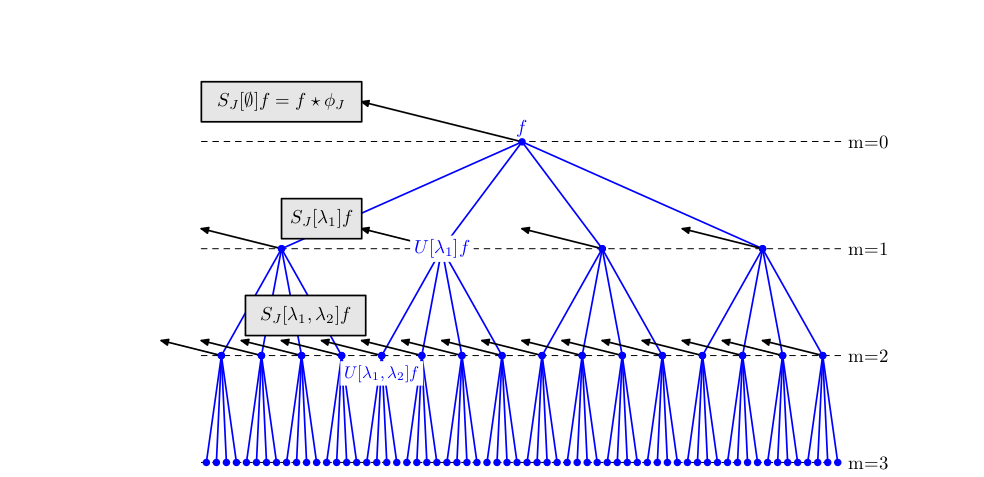
\includegraphics[width=0.8\textwidth]{img/ScatteringPropagator.png}
  \caption{Un PD $U_J$ aplicado a un punto de una señal $f(x)$ calcula $U[\lambda_1]f(x)=|f(x)\ast \psi_{\lambda_1}|$ y como salida a la capa $m=0$ se promedian los coeficientes que han dado $0$ (por tener $2^j<2^{-J}$) obteniendo como salida $S_J[\emptyset]f(x)=f(x)\ast \phi_{2^J}$ (como se puede ver en la flecha negra). Después se aplica de nuevo $U_J$ a cada coeficiente $U[\lambda_1]f(x)$ del paso anterior ($m=1$) $U[\lambda_1,\lambda2]f(x)$ obteniendo como salida $S_J[\lambda_1]f(x)=U[\lambda_1]f(x) \ast \phi_{2^J}$. Se repite este proceso de manera recursiva para cada coeficiente $U[p]f(x)$ y obteniendo como resultado $S_J[p]f(x)=U[p]f(x) \ast \phi_{2^J}$. Imagen extraída de \cite{bruna2013invariant}.}
  \label{fig:arbol_propag}
\end{figure}


\subsection{Diferencias y similitudes con una CNN}


Las operaciones de la transformada de dispersión que hemos descrito siguen la estructura general de la red neuronal convolucional introducida por LeCun \cite{lecun2015deep}, pues se describen las redes convolucionales como una cascada de convoluciones (la transfomada de ondeletas $W[\lambda]$) y capas de "pooling" que usan funciones no lineales (el operador módulo $M[\lambda]$), las cuales se representan en este modelo como módulos de números complejos. También se puede considerar como un operador de \entrecomillado{pooling} la función $\phi_{2^J}$ que se emplea para agregar coeficientes y construir un operador invariante.

\medskip

\noindent Las redes neuronales convolucionales han sido empleadas con mucho éxito en tareas de reconocimiento de objetos o personas y usan normalmente kernels que no son predefinidos, sino que se aprenden mediante la técnica de back-propagation al entrenar la red. En cambio, en la modelización que se ha presentado las ondeletas que usamos son prefijadas y no se aprenden.

\medskip

\noindent Siguiendo con las similitudes entre ambos modelos, si $p$ es un camino de longitud $m$, entonces a $S_J[p] f(x)$ se le denomina coeficiente de orden $m$ a escala $2^J$, que en el caso de una CNN, equivaldría al tensor formado por los mapas de activación tras la convolución con el kernel de la capa $m$ de la red. 

\medskip


\subsection{Relación con herramientas clásicas de visión por computador}
\noindent Por otro lado, la modelización  con los algoritmos clásicos de visión por computador como \textbf{SIFT}  \cite{DistinctiveImageFeatures}, se usa para calcular puntos de interés en imágenes. Así, con la ondeletas apropiadas, los coeficientes de primer orden $S[\lambda_1] f$ serían equivalentes a los coeficientes del algoritmo. De hecho, en el artículo sobre el descriptor DAISY \cite{Daisy} se muestra cómo esos coeficientes son aproximados por $S_J[2^j r] f= | f \ast \psi_{2^j r} | \ast \phi_{2^J}(x)$, donde $\psi_{2^j r}$ es la derivada parcial de una Gaussiana calculada en imagen de escala $2^j$ de mayor calidad, para 8 rotaciones distintas $r$. El filtro para promediar $\phi_{2^J}$ es un filtro Gaussiano escalado.


\subsection{Operador no expansivo.}

\noindent El propagador $U_Jf=\lbrace A_Jf, \left(\left| W[\lambda]f\right|\right)_{\lambda\in\Lambda_J} \rbrace$ es no expansivo, porque la transformada de ondas $W_J$ es unitaria pues cumple las hipótesis de la Proposición \ref{unitario} y el módulo no es expansivo en el sentido de que $\|a|-|b\|\leq |a-b|$ para cualquier $(a,b)\in \mathbb{C}^2$. Esto es válido tanto si $f$ es real o compleja. Como consecuencia: 

\begin{align*} 
    \|U_J f-U_J h\|^2 &= \|A_J f-A_J h\|^2+\sum_{\lambda\in\Lambda_J} \left\| \; |W[\lambda]f|-|W[\lambda]h| \; \right\|^2 \\
    &\leq \left\| W_J f- W_J h \right\|^2 \leq \|f-h\|^2
\end{align*}

\noindent Al ser $W_J$ unitaria, tomando la función nula $h=0$ y siguiendo el mismo razonamiento anterior, también se comprueba que $\|U_J f\|=\|f\|$ por lo que el operador $U_J$ preserva la norma.

\medskip

\noindent Para todo conjunto de caminos $\Omega$, las normas de $S_J[\Omega]f$ y $U[\Omega]f$ son: 

$$\left|\left| S_J[\Omega]f \right|\right|^2=\sum_{p\in\Omega} \left|\left| S_J[p]f\right|\right|^2 \;\; y \;\; \left|\left|U[\Omega]f\right|\right|^2=\sum_{p\in\Omega} \left|\left| U[p]f\right|\right|^2$$

\noindent Como $S_J[\mathcal{P}_J]$ itera en $U_J$, que es no expansivo, la siguiente proposición prueba que $S_J[\Omega]f$ es también no expansivo. 

\begin{proposicion} \label{proposicion::NoExpansiva}
La transformada de dispersión de ventana es no expansiva: 

\begin{equation}
  \forall (f,h)\in L^2(\mathbb{R}^d)^2 \;\; \|S_J[\mathcal{P}_J]f-S_J[\mathcal{P}_J]h\| \leq \|f-h\|
\end{equation}
\end{proposicion}

\begin{proof}
Como $U_J$ es no expansiva, partiendo de \eqref{eq::1.5} que nos dice: 
$$U_J U[\Lambda_J^m]=\lbrace S_J[\Lambda_J^m]f,(U[\Lambda_J^{m+1}]f)_{\lambda\in\Lambda_J}\rbrace,$$

se tiene que:

\begin{align*}
    \|U[\Lambda_J^m]f-U[\Lambda_J^m]h\|^2 &\geq \|U_J U[\Lambda_J^m]f-U_J U[\Lambda_J^m]h\|^2 \\
    & = \|S_J[\Lambda_J^m]f - S_J[\Lambda_J^m]h\|^2 + \|U[\Lambda_J^{m+1}]f-U[\Lambda_J^{m+1}]h\|^2.
\end{align*}

\medskip

\noindent Si ahora sumamos en $m$ cuando tiende a $\infty$ se obtiene que: 

\begin{align*}
  \sum_{m=0}^{\infty}\|U[\Lambda_J^m]f-U[\Lambda_J^m]h\|^2 &\geq \sum_{m=0}^{\infty} \|S_J[\Lambda_J^m]f - S_J[\Lambda_J^m]h\|^2 + \sum_{m=0}^{\infty} \|U[\Lambda_J^{m+1}]f-U[\Lambda_J^{m+1}]h\|^2,\\
\end{align*}

\noindent que equivale a:

\begin{align*}
  \sum_{m=0}^{\infty}\|U[\Lambda_J^m]f-U[\Lambda_J^m]h\|^2 - \sum_{m=0}^{\infty} \|U[\Lambda_J^{m+1}]f-U[\Lambda_J^{m+1}]h\|^2 &\geq \sum_{m=0}^{\infty} \|S_J[\Lambda_J^m]f - S_J[\Lambda_J^m]h\|^2\\
\end{align*}

\noindent Si ahora nos fijamos en el lado izquierdo de la desigualdad, se cancelan todos los términos salvo $m=0$, y teniendo en cuenta que $\Lambda^0_J=\emptyset$ queda: 

\begin{align*}
  \|U[\Lambda_J^0]f-U[\Lambda_J^0]h\|^2 &= \|U[\emptyset]f-U[\emptyset]h\|^2 = \| f - h \|^2 \\
\end{align*}

\noindent Por otro lado para el miembro derecho de la desigualdad anterior, se tiene que

\begin{align*}
  \sum_{m=0}^{\infty} \|S_J[\Lambda_J^m]f - S_J[\Lambda_J^m]h\|^2 = \|S_J[\mathcal{P}_J]f - S_J[\mathcal{P}_J]h\|^2. \\
\end{align*}

\noindent Luego hemos probado que 

$$\|S_J[\mathcal{P}_J]f - S_J[\mathcal{P}_J]h\|^2 \leq \| f - h \|^2$$

\noindent y por lo tanto que la transfomada de dispersión de ventana es no expansiva. \qedhere
\end{proof}

\subsection{Conservación de la norma.}

En la \autoref{ch:seccion12} se obtuvo que cada coeficiente $U[\lambda]f=|f \ast \psi_\lambda|$ capturaba la energía de frecuencia de $f$ en una banda de frecuencia cubierta por $\widehat{\psi}_\lambda$ y propagaba dicha energía a frecuencias decrecientes, este hecho lo demuestra el siguiente resultado, mostrando que toda la energía del propagador de dispersión alncanza la frecuencia mínima $2^J$ y es atrapada por el filtro de paso bajo $\phi_ {2^J}$. La energía propagada tiende a $0$ conforme se incrementa la longitud del camino, y el teorema implica que $\|S_J[\mathcal{P}_J]f\|=\|f\|$. Esto se aplica también a funciones complejas en caminos negativos.

\medskip

\noindent Para la demostración de la conservación de la norma necesitamos unos resultados previos: 

\begin{lema} \label{lema::Cota_inferior}
  Si $h$ es una función tal que $h\geq 0$ entonces $\forall f \in L^2(\mathbb{R}^d)$: 
  
  \begin{equation}
    |f \ast \psi_\lambda | \ast h \geq \sup_{\eta \in \mathbb{R}^d} |f\ast \psi_\lambda \ast h_\eta | \; \; con \; h_\eta=h(x)e^{i\eta x}.
  \end{equation}
\end{lema}
  
\begin{proof}
  
  \begin{align*}
      |f \ast \psi_\lambda | \ast h (x) &= \int \left| \int f(v)\psi_\lambda(u-v)dv \right| h(x-u)du \\
      &=\int \left | \int f(v) \psi_\lambda(u-v) e^{i\eta(x-u)} h(x-u) dv \right| du \\
      &\geq \left | \int \int f(v) \psi_\lambda(u-v) e^{i\eta(x-u)} h(x-u) dv du \right| = \\
      &= \left | \int f(v) \int  \psi_\lambda(x-v-u')h(u') e^{i\eta u'}  du' dv \right| \\
      &= \left | \int f(v) \psi_\lambda \ast h_\eta(x-v) dv \right| = |f\ast \psi_\lambda \ast h_\eta|
  \end{align*}

  \noindent Donde se ha usado el cambio de variable $u'=x-u$ con Jacobiano igual a $1$.
\end{proof}

\noindent A continuación definimos el concepto de \entrecomillado{ondeleta admisible:}
\begin{definicion}
  Una ondeleta de dispersión se dice que es admisible si existe $\eta \in \mathbb{R}^d$ y una función $\rho \geq 0$, con $|\widehat{\rho}(\omega)| \leq |\widehat{\phi}(2\omega)|$ y $\widehat{\rho}(0)=1$, tal que la función: 

\begin{equation}\label{eq::1.6}
  \widehat{\Psi}(\omega)=|\widehat{\rho}(\omega - \eta)|^2 - \sum_{k=1}^{+\infty} k(1-|\widehat{\rho}(2^{-k}(\omega - \eta))|^2)
\end{equation}
  
\noindent satisface: 
\begin{equation} \label{eq::1.7}
  \alpha= \inf_{1\leq|w|\leq2} \sum_{j=-\infty}^{\infty} \sum_{r\in G} \widehat{\Psi} (2^{-j}r^{-1}\omega)|\widehat{\psi}(2^{-j}r^{-1}\omega)|^2>0.
\end{equation}

\end{definicion}

\noindent Con esta definición en mente podemos comprobar que se da el siguiente lema que demuestra que el propagador dispersa la energía progresivamente hacia bajas frecuencias.

\begin{lema} \label{lema::Admisibilidad}
Si \eqref{eq::1.7} se satisface y 

\begin{equation}
  \|f\|_w^2=\sum_{j=0}^\infty \sum_{r\in G^+} j \|W[2^j r] f\|^2 < \infty
\end{equation}

\noindent entonces se tiene: 

\begin{equation}\label{eq::1.9}
  \frac{\alpha}{2}\|U[\mathcal{P}_J]f\|^2 \geq \max (J+1,1) \|f\|^2 + \|f\|_w^2.
\end{equation}

\end{lema}

\medskip

\noindent La demostración de lema se encuentra en el apéndice A de \cite{GroupInvariantScattering}. No se ha incluido en este trabajo por tratarse de una demostración muy técnica y de gran complejidad.

\medskip

\noindent Con todos estos resultados podemos presentar el principal teorema de esta sección, que nos dará como resultado la preservación de la norma del operador de ventana:


\begin{teorema} \label{teoremaOndeletasAdmisibles}
\noindent Si las ondeletas son admisibles, entonces para toda $f\in L^2(\mathbb{R}^d)$ se tiene que
\begin{equation}  
  \lim_{m\rightarrow\infty} \|U[\Lambda_J^m]f \|^2=\lim_{m\rightarrow\infty} \sum_{n=m}^{\infty} \|S_J[\Lambda_J^n]f\|^2=0
\end{equation}

y

\begin{equation}
  \|S_J[\mathcal{P}_J]f\|=\|f\|.
\end{equation}

\end{teorema}

\begin{proof}
  Esta demostración tiene dos partes, la primera consistirá en demostrar que la condición \eqref{eq::1.6} implica que $\lim_{m\rightarrow \infty} \| U[\Lambda_J^m]f \|^2=0$. 
  
  \medskip

  \noindent La clave de esto reside en el Lema \ref{lema::Cota_inferior}, que nos da una cota inferior de $|f\ast\psi_\lambda|$ convolucionada con una función positiva. Como 

  $$ \| U[\mathcal{P}_J]f \|^2= \sum_{m=0}^{+\infty} \|U[\Lambda_J^m]f\|^2,$$

  \noindent si $\|f\|_w < \infty$ entonces \eqref{eq::1.9} implica que $\lim_{m\rightarrow\infty}\|U[\Lambda_J^m]f\|= 0$. Este resultado se extiende a $L^2(\mathbb{R}^d)$ por densidad. Como $\phi \in L^1(\mathbb{R}^d)$ y $\widehat{\phi}(0)=1$, cualquier $f\in L^2(\mathbb{R}^d)$ satisface $\lim_{n\rightarrow - \infty} \|f-f_n\|=0$, donde $f_n=f \ast \phi_{2^n}$ y $\phi_{2^n}=2^{-nd} \phi(2^{-n}x)$. Se demuestra por tanto que $\lim_{m\rightarrow \infty} \|U[\Lambda_J^m]f_n\|=0$ viendo que $\|f_n\|_w < \infty$. De hecho, 


  \begin{align*}
      \|W[2^jr]f_n\|^2 &= \int |\widehat{f}(\omega)|^2 |\widehat{\phi}(2^n \omega)|^2 |\widehat{\psi}(2^{-j}r^{-1}\omega)|^2 d\omega \\
      &\leq C 2^{-2n-2j} \int |\widehat{f}(\omega)|^2 d\omega,
  \end{align*}

  \noindent porque hay un momento en que $\psi$ desaparece, entonces $|\widehat{\psi}(\omega)|=O(|\omega|)$, y las derivadas de $\phi$ están en $L^1(\mathbb{R}^d)$ luego $|\omega\|\widehat{\phi}\omega|$ están acotadas. Por lo que se tiene que $\|f_n\|_w < \infty$.

  \medskip

  \noindent Como $U[\Lambda^m]$ es no expansiva, se tiene $\|U[\Lambda_J^m]f-U[\Lambda_J^m]f_n\| \leq \|f - f_n\|$, por lo que 

  $$\|U[\Lambda_J^m]f\| \leq \| f-f_n\| + \|U[\Lambda_J^m]f_n\|.$$

  \noindent Como $\lim_{n\rightarrow -\infty}\|f-f_n\|=0$ y $\lim_{m\rightarrow\infty}\|U[\Lambda_J^m]f_n\|=0$ tenemos que 

  $$\lim_{m\rightarrow\infty} \|U[\Lambda_J^m]f\|^2=0$$

  \noindent para toda $f \in L^2(\mathbb{R}^d)$. 

  \medskip

  \noindent \textbf{En segundo lugar} vamos a ver que las siguientes expresiones son equivalentes: 
  \begin{align*}
    \lim_{m\rightarrow \infty} \|U[\Lambda_J^m]f\|^2=0 \iff \lim_{m\rightarrow\infty} \sum_{n=m}^{\infty} \|S_J[\Lambda_J^n]f\|^2=0 \iff \|S_J[\mathcal{P}_J]f\|^2 = \|f\|.
  \end{align*}

  \noindent Primero probamos que 
  $$\lim_{m\rightarrow \infty} \|U[\Lambda_J^m]f\|^2=0 \iff \lim_{m\rightarrow\infty} \sum_{n=m}^{\infty} \|S_J[\Lambda_J^n]f\|^2=0.$$
  
  \noindent Como $\|U_J h\|=\|h\| \; \forall h \in L^2(\mathbb{R}^d)$ y $U_J U[\Lambda_J^n]f=\lbrace S_J[\Lambda_J^n]f,U[\Lambda_J^{n+1}]\rbrace$,

 \begin{equation} \label{eq::1.8}
  \|U[\Lambda_J^n]f\|^2=\|U_JU[\Lambda_J^n]f\|^2=\|S_J[\Lambda_J^n]f\|^2+\|U[\Lambda_J^{n+1}]f\|^2. 
 \end{equation}

  \noindent Sumando en $m\leq n < \infty$ se obtiene : 
  
  \begin{align*}
    \sum_{n=m}^\infty \|U[\Lambda_J^n]f\|^2=&\sum_{n=m}^\infty \|S_J[\Lambda_J^n]f\|^2 + \sum_{n=m}^\infty\|U[\Lambda_J^{n+1}]f\|^2 \\
    \Big\Updownarrow \\
    \sum_{n=m}^\infty \|U[\Lambda_J^n]f\|^2 -& \sum_{n=m}^\infty\|U[\Lambda_J^{n+1}]f\|^2 =\sum_{n=m}^\infty \|S_J[\Lambda_J^n]f\|^2  \\
  \end{align*}
  
  \noindent En el término de la izquierda se anulan entre si todos los sumandos salvo $n=m$, luego queda: 

  \begin{align*}
    \|U[\Lambda_J^m]f\|^2 =\sum_{n=m}^\infty \|S_J[\Lambda_J^n]f\|^2  \\
  \end{align*}
  \noindent Y tomando límites cuando $m\rightarrow \infty$
  \begin{align*}
    \lim_{m\rightarrow \infty}\|U[\Lambda_J^m]f\|^2 =\lim_{m\rightarrow \infty}\sum_{n=m}^\infty \|S_J[\Lambda_J^n]f\|^2.  \\
  \end{align*}

  \medskip

  \noindent Por otro lado, sumando en \eqref{eq::1.8} para $0\leq n < m$ se obtiene:

  \begin{align*}
    \sum_{n=0}^{m-1} \|U[\Lambda_J^n]f\|^2=&\sum_{n=0}^{m-1} \|S_J[\Lambda_J^n]f\|^2 +\sum_{n=0}^{m-1}\|U[\Lambda_J^{n+1}]f\|^2 \\
    \Big\Updownarrow \\
    \sum_{n=0}^{m-1} \|U[\Lambda_J^n]f\|^2 -& \sum_{n=0}^{m-1}\|U[\Lambda_J^{n+1}]f\|^2 = \sum_{n=0}^{m-1} \|S_J[\Lambda_J^n]f\|^2.  \\
  \end{align*}
  
  \noindent En el término de la izquierda se anulan entre si todos los sumandos salvo $n=0$, y teniendo en cuenta que $f=U[\Lambda_J^0]f$ queda:
  
  \begin{equation}
    \|f\|^2=\sum_{n=0}^{m-1} \|S_J[\Lambda_J^n]f\|^2 + \|U[\Lambda_J^m]f\|^2.
  \end{equation}

  \noindent Si ahora tomamos límite cuando $m\rightarrow \infty$ obtenemos: 
  \begin{align*}
    \lim_{m\rightarrow \infty}\|f\|^2 =\lim_{m\rightarrow \infty}\sum_{n=0}^{m-1} \|S_J[\Lambda_J^n]f\|^2 &+ \lim_{m\rightarrow \infty} \|U[\Lambda_J^m]f\|^2  \\
    \Big\Updownarrow \\
    \|f\|^2 =\sum_{n=0}^{\infty} \|S_J[\Lambda_J^n]f\|^2 &+ \lim_{m\rightarrow \infty} \|U[\Lambda_J^m]f\|^2  \\
    \Big\Updownarrow \\
    \|f\|^2 =\|S_J[\mathcal{P}_J]f\|^2 &+ \lim_{m\rightarrow \infty} \|U[\Lambda_J^m]f\|^2.  \\
  \end{align*}

  \noindent De manera que se puede apreciar claramente que  
  \begin{align*}
    \|f\|^2 =\|S_J[\mathcal{P}_J]f\|^2 + \lim_{m\rightarrow \infty} \|U[\Lambda_J^m]f\|^2  = \|S_J[\mathcal{P}_J]f\|^2 \iff \lim_{m\rightarrow \infty} \|U[\Lambda_J^m]f\|^2=0. \\
  \end{align*}

  \noindent Con lo que queda demostrado el teorema. \qedhere
\end{proof}

\subsection{Conclusiones extraídas del teorema}
\noindent La demostración muestra que el propagador dispersa la energía progresivamente a frecuencias menores. La energía de $U[p]f$ se concentra principalmente en los caminos de frecuencia decrecientes $p=(\lambda_k)_{k\leq m}$ para los que $|\lambda_{k+1}|<|\lambda_k|$.


\medskip

\noindent El decrecimiento de $\sum_{n=m}^\infty \| S_J[\Lambda_J^n]f\|^2$ nos sugiere que podemos descartar todos los caminos de longitud mayor que un cierto $m>0$. De hecho, en tareas de tratamiento de imágenes y audio el decrecimiento numérico de $\|S_J[\Lambda_J^n]f\|^2$ puede llegar a ser exponencial, lo que lleva a que en problemas de clasificación, por ejemplo, la longitud del camino se limite a $m=3$.

\medskip

\noindent El teorema además requiere de una transformada de ondeleta unitaria y admisible que satisfaga la condición de Littlewood-Paley $\beta \sum_{(j,r)\in \mathbb{Z}\times G}|\widehat{\psi}(2^jr\omega)|^2=1$. 

\medskip

\noindent Debe también existir una función $\rho \geq 0$ y un $\eta \in \mathbb{R}^d$ con $|\widehat{\rho}(\omega)|\leq |\widehat{\phi}(2\omega)|$ tal que: 

$$\sum_{(j,r)\in\mathbb{Z}\times G}|\widehat{\psi}(2^jr\omega)|^2|\widehat{\rho}(2^jr\omega-\eta)|^2$$

\noindent sea suficientemente grande para que $\alpha>0$. Esto se puede obtener como se indica en $(2.3)$, con $\psi(x)=e^{i\eta x}\Theta(x)$ y de hecho $\widehat{\psi}=\widehat{\Theta}(\omega-\eta)$, donde $\widehat{\Theta}$ y $\widehat{\rho}$ tienen su energía concentrada en los mismos dominos de frecuencia, que son bajos.

\endinput


\chapter{Invarianza por Traslaciones} \label{ch:seccion14}

\noindent Hasta ahora hemos definido el propagador de dispersión y hemos visto algunas propiedades como la conservación de la norma de la señal $f$. No obstante, aún queda por demostrar la invarianza por traslaciones.

\section{No expansividad del operador de ventana en conjuntos de caminos}
Vamos a demostrar en primer lugar que $||S_J[\mathcal{P}_J] f- S_J[\mathcal{P}_J] h ||$ es no expansiva cuando se incrementa $J$, y que de hecho converge cuando $J \rightarrow \infty$. Esto define una distancia límite que como veremos a continuación es invariante por traslaciones.

\medskip

\begin{proposicion}
\noindent Para $f,h \in L^2(\mathbb{R}^d)$ y $J\in \mathbb{Z}$ se cumple

\begin{equation} \label{eq::1.10}
  || S_{J+1} [\mathcal{P}_{J+1}]f- S_{J+1}[\mathcal{P}_{J+1}]h || \leq ||S_J[\mathcal{P}_J]f - S_J[\mathcal{P}_J]h ||. 
\end{equation}

\end{proposicion}

\begin{proof}

\noindent En primer lugar, vamos a transformar la condición que queremos demostrar en \eqref{eq::1.10} en otra equivalente y que será más fácil de probar.

\medskip

\noindent Si recordamos la definición de $\mathcal{P}_J$, era un conjunto de caminos finitos $p=(\lambda_1,\ldots,\lambda_m)$ tal que $\lambda_k\in\Lambda_J$ y $|\lambda_k|=2^{k}>2^{-J}$. Luego todo camino $p' \in \mathcal{P}_{J+1}$, puede ser unívocamente escrito como una extensión de un camino $p\in \mathcal{P}_J$ donde $p$ es el prefijo más grande de $p'$ que pertenece a $\mathcal{P}_J$, y $p'=p+q$ para algún $q\in \mathcal{P}_{J+1}$. De hecho, podemos definir el conjunto de todas las extensiones de $p\in \mathcal{P}_J$ en $\mathcal{P}_{J+1}$ como: 

\begin{equation}
  \mathcal{P}_{J+1}^{p}={p} \cup {p+2^{-J}r+p''} \; \; r\in G^{+},p''\in \mathcal{P}_{J+1}.
\end{equation}

\noindent Esto define una partición disjunta de $\mathcal{P}_{J+1}=\cup_{p \in \mathcal{P}_J} \mathcal{P}_{J+1}^{p}$. Y deberíamos probar que dichas extensiones son no expansivas,

\begin{equation}\label{eq::1.11}
  \sum_{p' \in \mathcal{P}_{J+1}^p} || S_{J+1}[p']f-S_{J+1}[p']h||^2 \leq ||S_{J}[p]f-S_J [p]h||^2.
\end{equation}

\noindent Finalmente, si nos fijamos, la condición \eqref{eq::1.11} equivale a \eqref{eq::1.10} sumando en todo $p\in \mathcal{P}_J$, luego probando \eqref{eq::1.11} tendríamos el resultado que buscamos. 


\medskip


\noindent Para ello vamos a necesitar el siguiente lema:

\begin{lema}
  Para ondeletas que satisfacen la propiedad presentada en la Proposición \ref{unitario}, para toda función \textbf{real} $f\in L^2(\mathbb{R}^d)$ y todo $q \in \mathbb{Z}$ se verifica: 

  $$\sum_{-q\geq l > -J} \sum_{r \in G^+} || f \ast \psi_{2^lr}||^2 + || f \ast \phi_{2^J}||^2 = || f \ast \phi_{2^q} ||^2.$$

\end{lema}

\begin{proof}

  \noindent En primer lugar vamos a ver que de la Proposición \ref{unitario} se deduce la siguiente expresión: 

  $$|\widehat{\phi}(2^J \omega)|^2 + \sum_{-q\geq l > -J} \sum_{r \in G^+}|\widehat{\psi}(2^{-l}r^{-1} \omega)|^2=|\widehat{\phi}(2^q \omega) |^2.$$

  \noindent Para ello, de la expresión

  \begin{align*}
    \frac{1}{2} \sum_{j=-\infty}^\infty \sum_{r \in G} |\widehat{\psi}(2^{-j}r^{-1}\omega)|^2=1 & \; \; y
    \;\;|\widehat{\phi}(\omega)|^2= \frac{1}{2} \sum_{j=-\infty}^0 \sum_{r\in G} |\widehat{\psi}(2^{-j}r^{-1}\omega)|^2,
  \end{align*}

  \noindent se tiene de la misma forma que vimos en la demostración de la Proposición \ref{unitario} que:

  $$\forall J \in \mathbb{Z} \; \; \; \left|\widehat{\phi}\left(2^J\omega\right)\right|^2 + \frac{1}{2} \sum_{j>-J,r\in G}\left|\widehat{\psi}\left(2^{-j}r^{-1}\omega\right)\right|^2=1. $$

  \noindent Y partiendo el sumatorio obtenemos que: 

  $$\left|\widehat{\phi}\left(2^J\omega\right)\right|^2 + \frac{1}{2}  \sum_{-q \geq j >-J,r \in G}\left|\widehat{\psi}\left(2^{-j}r^{-1}\omega\right)\right|^2= \frac{1}{2} \sum_{j>-q,r \in G}\left|\widehat{\psi}\left(2^{-j}r^{-1}\omega\right)\right|^2=|\widehat{\phi}(2^q \omega)|^2.$$
  
  \noindent Ahora multiplicamos la expresión anterior por $|\widehat{f}(\omega)|^2$, 
  
  $$\left|\widehat{f}(\omega)\right|^2 \left|\widehat{\phi}\left(2^J\omega\right)\right|^2 + \frac{1}{2} \sum_{-q \geq j >-J,r \in G} \left|\widehat{f}(\omega)\right|^2 \left|\widehat{\psi}\left(2^{-j}r^{-1}\omega\right)\right|^2=\left|\widehat{f}(\omega)\right|^2 \left|\widehat{\phi}(2^q \omega)\right|^2.$$

  \noindent Integramos en $\omega$, 

  \begin{align*}
    \int \left|\widehat{f}(\omega)\right|^2 \left|\widehat{\phi}\left(2^J\omega\right)\right|^2 d\omega &+ \frac{1}{2} \sum_{-q \geq j >-J,r \in G} \int \left|\widehat{f}(\omega)\right|^2 \left|\widehat{\psi}\left(2^{-j}r^{-1}\omega\right)\right|^2 d\omega \\ 
    &=\int \left|\widehat{f}(\omega)\right|^2 \left|\widehat{\phi}(2^q \omega)\right|^2 d\omega.
  \end{align*}


  \noindent Ahora estamos en condiciones de aplicar el \autoref{Teorema::Convolucion}, y nos queda que la expresión anterior equivale a: 

  \begin{align*}
    \int \left|(f \ast \phi_{2^J}) (x)\right|^2 dx + \sum_{-q \geq j >-J,r \in G} \int \left|(f \ast \psi_{2^{j}r})(x)\right|^2 dx=\int \left|(f \ast \phi_{2^q}) (x)\right|^2 dx,
  \end{align*}

  \noindent y teniendo en cuenta que $f$ es real y por lo tanto que $||f \ast \psi_{2^j r}||= ||f \ast \psi_{2^j -r}||$ junto con la defnición de la norma de $L^2(\mathbb{R}^d)$, se tiene  

  \begin{align*}
    \sum_{-q\geq l > -J} \sum_{r \in G^+} || f \ast \psi_{2^lr}||^2 + || f \ast \phi_{2^J}||^2 = || f \ast \phi_{2^q} ||^2& \\ 
    &\qedhere
  \end{align*} 

\end{proof}


\noindent Vamos ahora a usar el lema anterior con la función $g=U[p]f-U[p]h$ junto con que $U[p]f\ast \phi_{2^J}=S_J[p]f$. De esta forma se tiene:

$$||g \ast \phi_{2^{J+1}} ||^2 + \sum_{r\in G^+} || g\ast \psi_{2^{-J}r} ||^2=||g \ast \phi_{2^J}||^2.$$

\noindent Así, sustituyendo el valor de $g$ por el que hemos definido antes y aplicando la propiedad distributiva de la convolución, obtenemos:

\begin{align*}
  ||U[p]f \ast \phi_{2^J} -U[p]h \ast \phi_{2^J}||^2 = &||U[p]f \ast \phi_{2^{J+1}} - U[p]h \ast \phi_{2^{J+1}} ||^2 \\
  & + \sum_{r\in G^+} || U[p]f\ast \psi_{2^{-J}r} -U[p]h \ast \psi_{2^{-J}r}||^2.
\end{align*}

\noindent Y esto equivale a

\begin{align*}
  ||S_{J}[p]f-S_J[p]h||^2 = &|| S_{J+1}[p]f-S_{J+1}[p]h||^2 \\
  & + \sum_{r\in G^+} || U[p]f\ast \psi_{2^{-J}r} -U[p]h \ast \psi_{2^{-J}r}||^2.
\end{align*}

\noindent Aplicando ahora la propiedad de la norma de que $\|g - h \| \geq \| |g| - |h| \|$ y como $$|U[p]f\ast\psi_{2^{-J}r}|=U[p+2^{-J}r]f,$$ se concluye que

\begin{align*}
    ||S_{J}[p]f-S_J[p]h||^2 \geq & || S_{J+1}[p]f-S_{J+1}[p]h||^2 \\
    & + \sum_{r\in G^+} ||U[p+2^{-J}r]f-U[p+2^{-J}r]h||^2.
\end{align*}


\noindent Como $S_{J+1}[\mathcal{P}_{J+1}]U[p+2^{-J}r]f=\lbrace S_{J+1} [p+2^{-J}r+p'']\rbrace_{p''\in\mathcal{P}_{J+1}}$  y $S_{J+1}[\mathcal{P}_{J+1}]f$ es no expansiva por la Proposición \ref{proposicion::NoExpansiva}, usando la desigualdad anterior podemos escribir

\begin{align*}
    ||S_{J}[p]f - S_J[p]h||^2 \geq & ||S_{J+1}[p]f-S_{J+1}[p]h||^2 \\
    & + \sum_{p''\in \mathcal{P}_{J+1}} \sum_{r\in G^+} || S_{J+1}[p+2^{-J}r+p'']f- S_{J+1}[p+2^{-J}r+p'']h||^2,
\end{align*}

\noindent y en particular

\begin{align*}
  ||S_{J}[p]f - S_J[p]h||^2 \geq & \sum_{p''\in \mathcal{P}_{J+1}} \sum_{r\in G^+} || S_{J+1}[p+2^{-J}r+p'']f- S_{J+1}[p+2^{-J}r+p'']h||^2,
\end{align*}

\noindent que demuestra \eqref{eq::1.11}. \qedhere
\end{proof}


\section{Invarianza por traslaciones}

\noindent La proposición anterior nos demuestra que $||S_J[\mathcal{P}_J]-S_J[\mathcal{P}_J]h||$ es positivo y no creciente cuando $J$ se incrementa, y de hecho converge. Como $S_J[\mathcal{P}_J]$ es no expansiva, el límite también lo es: 

$$\forall f,h \in L^2(\mathbb{R}^d) \lim_{J\rightarrow\infty} ||S_J[\mathcal{P}_J]f-S_{J}[\mathcal{P}_J]h|| \leq ||f-h||.$$

\medskip

\noindent Para ondeletas de dispersión admisibles que satisfacen \eqref{eq::1.7}, el \autoref{teoremaOndeletasAdmisibles} nos demuestra que si $||S_J[\mathcal{P}_J]f||=||f||$ entonces $\lim_{J\rightarrow\infty}||S_J[\mathcal{P}_J]f||=||f||$. El siguiente teorema demuestra que el límite es invariante por traslaciones, pero para la demostración del teorema necesitaremos dos resultados auxiliares:

\begin{lema} \label{lemma:Schur}
  Para cualquier operador $Kf(x)=\int f(u)k(x,u)du \; \in L^2(\mathbb{R}^d)$ se tiene 

  $$\int |k(x,u)| dx \leq C,$$

  \noindent con $C >0$, y además 

  $$\int |k(x,u)|du \leq C \implies ||K||\leq C.$$

  \noindent Donde $||K||$ es la norma en $L^2(\mathbb{R}^d)$ de $K$.
\end{lema}

\medskip

\noindent Para la demostración del lema anterior se necesita el Lema de Schur \cite{SchurLemma}. Debido a que se trata de un lema auxiliar que emplearemos para la demostración del teorema principal de la sección, no lo demostraremos.
 
\begin{lema} \label{lema::constante}
  Existe una constante $C$ tal que para todo $\tau \in \C^2(\mathbb{R}^d)$ con $||\nabla \tau ||_\infty \leq \frac{1}{2}$ se tiene que 
  
  $$||L_\tau A_J f - A_J f|| \leq C ||f||2^{-J}||\tau||_{\infty}.$$
\end{lema}

\begin{proof}

  \noindent En esta prueba, vamos a necesitar el Lema \ref{lemma:Schur}. 

  \medskip

  \noindent El operador norma de $k_J=L_\tau A_J - A_J$ se calcula aplicando el lema de Schur a su kernel,

  $$k_J(x,u)=\phi_{s^J}(x-\tau(x)-u)-\phi_{2^J}(x-u).$$

  \noindent Si nos fijamos en la expresión anterior, cuando $x=0=u$ se tiene que: 

  $$k_J(0,0)=\phi_{2^J}(0)-\phi_{2^J}(0)=0.$$

  \noindent Si ahora calculamos su polinomio de Taylor de primer orden centrado en el $(0,0)$ se obtiene: 

  $$k_J=k_J(0,0)+\int_0^1 \nabla \phi_{2^J} (x-t\tau(x)-u)\tau(x). dt$$

  \noindent Si ahora calculamos el módulo obtenemos que:

  \begin{align*}
    |k_J|&=|k_J(0,0)+\int_0^1 \nabla \phi_{2^J} (x-t\tau(x)-u)\tau(x) dt| \\
    &\leq |k_J(0,0)|+\left|\int_0^1 \nabla \phi_{2^J} (x-t\tau(x)-u)\tau(x) dt \right| \\
    & \leq \left|\int_0^1 \nabla \phi_{2^J} (x-t\tau(x)-u)\tau(x) dt \right| \\ 
    & \leq \int_0^1 \left| \nabla \phi_{2^J} (x-t\tau(x)-u)\tau(x)  \right|dt= |\tau(x)|\int_0^1 \left| \nabla \phi_{2^J} (x-t\tau(x)-u)\right|dt  \\ 
    & \leq ||\tau(x)||_\infty \int_0^1 \left| \nabla \phi_{2^J} (x-t\tau(x)-u)\right|dt.
  \end{align*}

  \noindent Si ahora integramos en $u$ y aplicamos el teorema de Fubini para itercambiar las integrales del lado derecho de la desigualdad obtenemos:

  \begin{align*}
    \int |k_J| du &\leq ||\tau(x)||_\infty \int \int_0^1 \left| \nabla \phi_{2^J} (x-t\tau(x)-u)\right|dt \; du = ||\tau(x)||_\infty \int_0^1 \int  \left| \nabla \phi_{2^J} (x-t\tau(x)-u)\right| du \; dt. 
  \end{align*}

  \noindent por otro lado, vamos a comprobar que 
  $$\nabla\phi_{2^J}(x)=2^{-dJ-J} \nabla \phi(2^{-J}x).$$

  \noindent Para ello debemos recordar que $\phi_{2^J}(x)=2^{-dJ}\phi(2^{-J}x)$ luego

  \begin{align*}
    \nabla \phi_{2^J}(x) &= \nabla(2^{-dJ}\phi(2^{-J}x)) \\
    &= 2^{-dJ} \nabla(\phi(2^{-J}x)).
  \end{align*}

  \noindent Si nos fijamos, debido a que $x$ está multiplicado por $2^{-J}$ en cada componente del vector, siempre que derivemos con respecto a alguna componente, vamos a poder sacar como factor común $2^{-J}$ por lo tanto:

  \begin{align*}
    \nabla \phi_{2^J}(x) = 2^{-dJ-J} \nabla(\phi(2^{-J}x)).
  \end{align*}

  \noindent De esta forma, realizando un cambio de variable obtenemos: 

  \begin{align*}
    \int |k_J| du &\leq ||\tau(x)||_\infty  2^{-dJ-J} \int \left| \nabla \phi (2^J u')\right|du' \\
    & = 2^{-J} ||\tau(x)||_\infty ||\nabla\phi||_1. 
  \end{align*}

  \noindent Si ahora realizamos el mismo procedimiento integrando en $x$ en vez de en $u$ tenemos que 

  \begin{align*}
    \int |k_J(x,u)| dx &\leq ||\tau(x)||_\infty \int_0^1 \int \left| \nabla \phi_{2^J} (x-t\tau(x)-u)\right| dx \; dt
  \end{align*}

  \noindent Ahora, aplicamos el cambio de variable $v=x - t\tau(x)$ y calculamos su Jacobiano

  \begin{align*}
    Jv& =J(x-t\tau(x))=J(x)-J(t\tau(x)) \\
    & = Id - tJ(\tau(x)) \\
    & = Id - t\nabla \tau(x).
  \end{align*}

  \noindent Vamos a buscar una cota para el determinante del Jacobiano

  \begin{align*}
    |J| & =(1-t\tau(x))^d \\
    & \geq (1-||\tau||_\infty)^d \\
    & \geq 2^{-d}.
  \end{align*}

  \noindent Aplicando ahora el cambio de variable a la integral

  \begin{align*}
    \int |k_J(x,u)| dx &\leq ||\tau(x)||_\infty 2^d \int_0^1 \int \left| \nabla \phi_{2^J} (v-u)\right| dv \; dt \\
    &= 2^{-J} ||\tau||_\infty ||\nabla \phi ||_1 2^{d}.
  \end{align*}

  \noindent De las dos cotas superiores obtenidas esta es la mayor, por lo que aplicamos el lema de Schur a esta y terminamos la demostración del lema

  $$ ||L_{\tau} A_J - A_J || \leq 2^{-J+d} ||\nabla \phi ||_1 ||\tau||_\infty. \;\;\; \qedhere$$
\end{proof}


\noindent Con esto ya tenemos todas las herramientas necesarias para enunciar y demostrar el teorema central de esta sección, que nos garantiza que el operador que estamos construyendo y que modeliza una red neuronal convolucional, es invariante por traslaciones.

\begin{teorema} \label{invarianzaTraslaciones}
Para ondeletas de dispersión admisibles se tiene que 

$$\forall f \in L^2(\mathbb{R}^d), \; \forall c\in \mathbb{R}^d \;\;\; \lim_{J\rightarrow \infty}||S_J[\mathcal{P}_J] f-S_J[\mathcal{P}_J] L_cf||=0.$$
\end{teorema}

\begin{proof}

\noindent Fijamos $f\in L^2(\mathbb{R}^d)$. Teniendo en cuenta la conmutatividad $S_J[\mathcal{P}_J] L_cf = L_cf S_J[\mathcal{P}_J]$ y la definición $S_J[\mathcal{P}_J]f=A_J U[\mathcal{P}_J]f$, obtenemos

\begin{align*}
    ||S_J[\mathcal{P}_J] L_cf - S_J[\mathcal{P}_J]f || &= ||L_c A_J U[\mathcal{P}_J]f - A_J U[\mathcal{P}_J]f|| \\
    &\leq ||L_c A_J - A_J|| ||U[\mathcal{P}_J]f||.
\end{align*}

\medskip

\noindent Si ahora aplicamos el Lema \ref{lema::constante} con $\tau=c$, se tiene que $||\tau||_\infty=|c|$ y además

$$||L_c A_J - A_J|| \leq C 2^{-J} |c|.$$

\noindent Y si tenemos en cuenta esto en la expresión anterior nos da que: 

\begin{align*}
  ||S_J[\mathcal{P}_J] L_cf - S_J[\mathcal{P}_J]f || & \leq ||L_c A_J - A_J|| ||U[\mathcal{P}_J]f|| \\
  & \leq C 2^{-J} |c| ||U[\mathcal{P}_J]f||
\end{align*}

\noindent Como la admisibilidad de la condición \eqref{eq::1.7} se satisface, en el Lema \ref{lema::Admisibilidad} se demuestra en \eqref{eq::1.9} que para $J>1$ se cumple

$$\frac{\alpha}{2}||U[\mathcal{P}_J]f||^2 \leq (J+1)||f||^2+||f||^2_w.$$

\noindent Y de esta expresión podemos sacar una cota superior para $||U[\mathcal{P}_J]f||$: 

\begin{align*}
  ||U[\mathcal{P}_J]f||^2 \leq ((J+1)||f||^2+||f||^2_w) 2 \alpha^{-1}
\end{align*}

\noindent Si $||f||_w < \infty$ entonces elevando al cuadrado en la desigualdad anterior, tenemos

$$||S_J[\mathcal{P}_J] L_cf - S_J[\mathcal{P}_J]f ||^2 \leq ((J+1)||f||^2+||f||_w^2)C^2 2 \alpha^{-1} 2^{-2J} |c|^2,$$

\noindent y tomando límite en ambos lados cuando $J\rightarrow \infty$ tenemos que 

\begin{align*}
  \lim_{J\rightarrow \infty} ||S_J[\mathcal{P}_J] L_cf - S_J[\mathcal{P}_J]f ||^2 &\leq \lim_{J\rightarrow \infty} ((J+1)||f||^2+||f||_w^2)C^2 2 \alpha^{-1} 2^{-2J} |c|^2 \\
  &= 0.
\end{align*}

\noindent Luego $\lim_{J\rightarrow\infty}||S_J[\mathcal{P}_J] L_cf - S_J[\mathcal{P}_J]f ||=0$.

\medskip

\noindent Finalmente vamos a probar ahora que el límite anterior se da $\forall f \in L^2(\mathbb{R}^d)$, con un argumento similar al de la prueba del \autoref{teoremaOndeletasAdmisibles}. Cualquier $f\in L^2(\mathbb{R}^d)$ se puede escribir como el límite de una sucesión de funciones $\lbrace f_n \rbrace_{n\in\mathbb{N}}$ con $||f_n||_w < \infty$, y como $S_J[\mathcal{P}_J]$ es no expansivo y $L_c$ es unitario, usando la desigualdad triangular, deducimos que 

$$||L_c S_J[\mathcal{P}_J]f-S_J[\mathcal{P}_J]f|| \leq ||L_c S_J [\mathcal{P}_J]f_n -S_J[\mathcal{P}_J]f_n|| + 2||f-f_n||.$$

\noindent Haciendo tender $n \rightarrow \infty$ se prueba que $\lim_{J\rightarrow \infty}||S_J[\mathcal{P}_J] f-S_J[\mathcal{P}_J] L_cf||=0$ con lo que acaba la demostración. \qedhere
\end{proof}


\endinput


\chapter{Conclusiones y Trabajos futuros}

\noindent En el primer capítulo dimos una introducción a las \textbf{CNN} y establecimos dos objetivos principales:

\begin{itemize}
  \item Tratar de dar una posible modelización matemática para una CNN.
  \item Demostrar la propiedad básica de la invarianza por traslaciones. 
\end{itemize}


\medskip

\noindent En primer lugar expusimos el problema de conseguir un operador adecuado que se pudiera aplicar de manera recursiva del mismo modo que hacen las CNN. Para ello se llegó a la conclusión de que dicho operador debía ser \textbf{invariante por traslaciones} y \textbf{Lipschitz-continuo} bajo la acción de difeomorfismos y vimos que debíamos rechazar el operador módulo de la transfomada de Fourier como candidato por no cumplir esta segunda propiedad. 

\medskip

\noindent Una vez rechazado el operador anterior vimos que la alternativa más prometedora era la de usar una transformada de Ondeletas, en concreto la de \textbf{Littlewood-Paley}:

\begin{equation}
  \forall x \in  \mathbb{R}^d \;\; W[\lambda]f(x)= f \ast \psi_\lambda(x)=\int f(u)\psi_\lambda(x-u) du .
\end{equation}

\noindent Este operador, al contrario que el módulo de la transformada de Fourier, es Lipschitz-continuo bajo la acción de difeomorfismos, pero produce coeficientes que no son invariantes por traslaciones. Para ello se necesita la ayuda de un operador no lineal auxiliar $M[\lambda]W[\lambda]f=|W[\lambda]f|$ y vimos que usando el módulo conseguíamos obtener un operador invariante por traslaciones definido en cualquier camino $p \in \mathcal{P}_\infty$ como:

\begin{equation}
  \overline{S}f(p)=\int_{\mathbb{R}^d}U[p]f(x)dx 
\end{equation} 

\medskip

\noindent No obstante, en la práctica se empleará el operador de ventana:

\begin{equation}
  S_J[p]f(x)=\left| |f \ast \psi_{\lambda_1} | \ast \psi_{\lambda_2} | \ldots | \ast \psi_{\lambda_m} \right| \ast \phi_{2^J}(x).
\end{equation}

\noindent Con este operador se consigue definir el que será la modelización de una CNN, y que además tiene unas propiedades deseables como la preservación de la norma o que es un operador no expansivo. Finalmente, con la modelización propuesta (el operador de ventana) se comprueba que no es expansivo en conjuntos de caminos a medida que decrece el umbral y con esta propiedad se consigue demostrar la invarianza por traslaciones del operador.

\medskip

\noindent Llegados a este punto podemos afirmar haber conseguido todos los objetivos que nos habíamos marcado. Sin embargo el camino para lograrlos ha sido complicado y ha estado marcado por la consecución de retos menores que me han hecho aprender mucho sobre conceptos que se explicaron durante el grado y otros totalmente. Es la prmiera vez que me enfrento a un trabajo de iniciación a la investigación, y por lo tanto en muchas situaciones me he visto envuelto de conceptos que no comprendía del todo y de los cuales no había mucha información viéndome en la necesidad clasificar y seleccionar lo mejor posible la información siempre pensando en los objetivos marcados. 

\medskip

\noindent En primer lugar tuve que recordar conceptos básicos del análisis de Fourier como son el cálculo de series de Fourirer y transformada de Fourier así como sus interpretaciones y aplicaciones. Por otro lado tuve que recordar conceptos de análisis como son la Lipschitz-continuidad y con esto pude entender y explicar la demostración de que el módulo de la transformada de Fourier no es lipschitz-continuo bajo la acción de difeomorfismos. También he aprendido teoremas conocidos en el ámbito del análisis de Fourier como son la fórmula de Plancharel o el Teorema de convolución de la transformada de Fourier. 

\medskip

\noindent Todas estas herramientas me han permitido introducirme en el mundo de las ondeletas, un mundo desconocido para mi y que es esencial en áreas de conocimiento como el procesamiento de señales y la visión por computador. Tuve que aprender y entender el concepto de ondeleta y transformada de ondeletas, y tuve que realizar una investigación sobre el tratamiento de señales (especialmente de imágenes) por medio de estas heramientas.

\medskip

\noindent Por otro lado, esta investigación me ha ayudado a comprender mejor el funcionamiento de una red neuronal convolucional y las posibles motivaciones matemáticas y propiedades subyacentes. Este tipo de estudio, de nuevo da sentido y sirve como nexo de unión a los dos grados que he cursado. Me he habituado a consultar y leer publicaciones matemática que trataran sobre estos temas, una destreza que considero de vital importancia y que sin duda será de gran utilidad para el futuro.

\endinput

\cleardoublepage\part{Localización de landmarks cefalométricos por medio de técnicas de few-shot learning}
% !TeX root = ../libro.tex
% !TeX encoding = utf8

\chapter{Introducción}  \label{ch:Introduccion_informatica}

\noindent Hoy en día vivimos en una sociedad en la que la tecnología se encuentra presente en prácticamente todas las tareas y disciplinas. Particularmente, en los últimos años hemos podido ver cómo el desarrollo \textbf{Inteligencia Artificial} ha permitido que tareas que antes se consideraban lentas o complicadas puedan realizarse rápidamente y con precisión con ayuda de un ordenador. En cambio, hay otras tareas que todavía resultan complicadas de resolver de forma rápida tanto para expertos en la materia como para ordenadores. Es dentro de este conjunto dónde se va a desarrollar el presente trabajo, pues como veremos a continuación y en posteriores secciones apenas hay publicaciones relacionadas con el tema. En particular se desarrollará en el ámbito de las ciencias forenses, que explicaremos a continuación.

\medskip

\noindent Las \textbf{ciencias forenses} son aquellas que aplican el método científico a hechos presuntamente delictivos con la finalidad de aportar pruebas a efectos judiciales. Dentro de este campo destacan principalmente dos disciplinas: 

\begin{itemize}
    \item La \textbf{Criminalística}: disciplina encargada del descubrimiento y verificación científica de presuntos hechos delictivos y quienes los cometen.
    \item La \textbf{Medicina Forense}: disciplina encargada de determinar el origen de las lesiones, las caisas de muerte o la identificación de seres humanos vivos o muertos.
\end{itemize}

\medskip

\noindent Dentro de la medicina forense se encuentra la \textbf{antropología forense}, que principalmente se encarga de la identificación de personas a partir de restos óseos. Y es en este ambiente dónde se encuentra el proceso que da sentido a este trabajo.


\section{Descripción del problema}

\noindent Los antropólogos forenses emplean diversas técnicas para la identificación de personas a partir de restos óseos como son la reconstrucción de huesos, el cotejo fotográfico con el cráneo o el análisis de imágenes. De entre estas técnicas, destaca la \textbf{Superposición Craneofacial} por ser la que se encuentra más relacionada con el fin de este trabajo. Se trata de una técnica de identificación forense mediante la cual se comparan imágenes de la persona difunta (imágenes se le denominan imágenes ante-mortem) con una representación 3D de un cráneo candidato, con el fin de determinar si el cráneo pertenece a la persona de las imágenes o no. Se distinguen cuatro etapas en el proceso: 

\begin{enumerate}
    \item Se recogen todos los datos necesarios para el proceso. Se recogen todas las imágenes disponibles de los sujetos ante-mortem, se realiza un escaneo $3D$ de los cráneos candidatos y se realiza el marcado de \textit{landmarks} o puntos de referencia. 
    
    \medskip
    
    \noindent El marcado de landmarks se realiza \textbf{de acuerdo a correspondencias morfológicas} tanto en la cara del sujeto en las imágenes como en el modelo $3D$ del cráneo candidato, de manera que cada punto marcado sobre el rosto tiene un homólogo marcado sobre el cráneo. Estos puntos de referencia reciben el nombre de \textbf{puntos craneométricos} cuando se marcan sobre el cráneo y \textbf{puntos cefalométricos} cuando se marcan sobre el rostro.
    \item Análisis morfológico y morfométrico. En esta etapa se realiza la selección de parejas imagen modelo $3D$ sobre las que realizar la superposición craneofacial.
    \item Se realiza la superposición cráneo-cara por parte del experto con ayuda de alguna herramienta como puede ser photoshop tratando de hacer corresponder cada landmark cefalométrico con su homólogo craneométrico.
    \item Se realiza la toma de decisiones en función de la bondad de los ajustes realizados.
\end{enumerate}

\begin{figure}[!h]
    \centering
    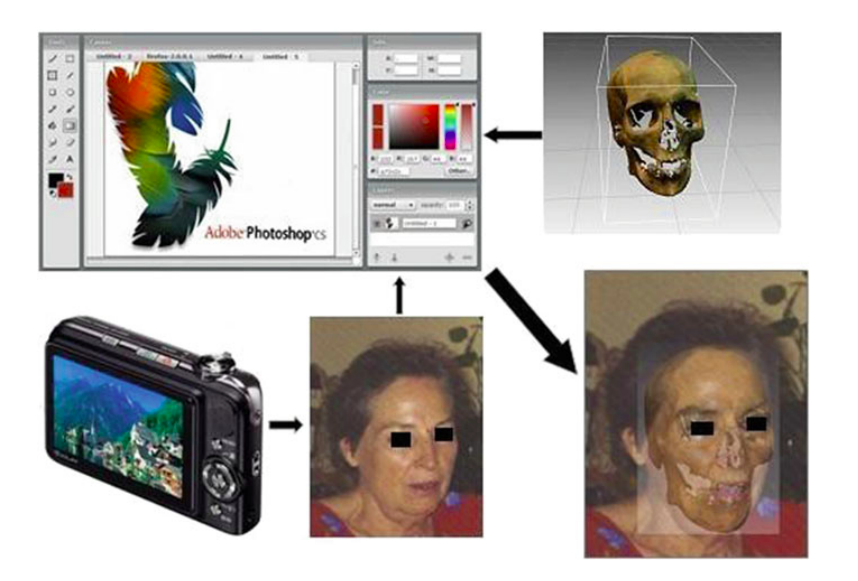
\includegraphics[width=0.8\textwidth]{img/ejemplo_SCF_intro.png}
    \caption{Ejemplo del proceso a seguir por el antropólogo forense en la superposición cráneo facial. Imagen extraida de \cite{damas2020handbook}.}
\end{figure}

\medskip

\noindent Sin embargo, esta tarea no es sencilla por factores diversos a tener en cuenta como son la grasa, la calidad de la imagen y el tejido blando facial que separa el punto craneométrico de su homólogo cefalométrico y que se traduce en una ligera traslación del punto. El desplazamiento ocasionado por el tejido blando facial no es constante ni se produce siempre en la misma dirección. Estos problemas, ocasionan que el experto forense tarde mucho en la tarea del marcado de landmarks. Una vez determinados los landmarks, un algoritmo automático puede encargarse de realziar el solapamiento del cráneo 3D y la imagen 2D acelerando el proceso y ahorrando tiempo en esta tarea al experto.

\begin{figure}[!h]
    \centering
    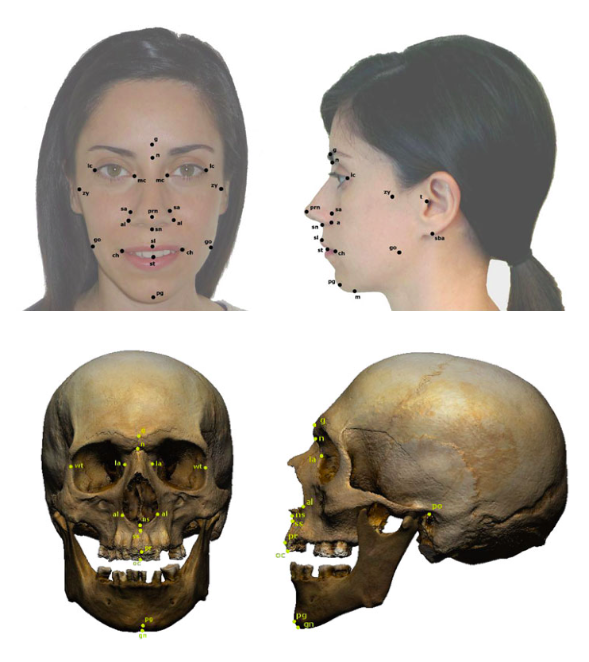
\includegraphics[width=0.9\textwidth]{img/marcado_landmarks.png}
    \caption{En esta imagen podemos ver algunos de los landmarks que se van a estudiar marcados tanto en rostro (cefalométricos) como en cráneo (craneométricos). Imagen extraida de \cite{damas2020handbook}.}
\end{figure}


\newpage

\noindent En este trabajo se estudiarán un total de $30$ landmarks, que son los siguientes: 

\begin{center}
    \begin{tabular}{ |c|l|l|c| } 
        \hline
         & \textbf{Landmarks} & \textbf{notación} \\
        \hline
        1 & Menton & Me \\ 
        2 & Gnathion & Gn \\ 
        3 & Pogonion & Pg \\ 
        4 & Prosthion & Pr \\ 
        5 & Labiale Superius & Ls \\ 
        6 & Subnasale & Sn \\ 
        7 & Nasion & N \\ 
        8 & Glabella & G’ \\ 
        9 & Vertex & v \\ 
        10 & Left Gonion & GoL \\ 
        11 & Right Gonion & GoR\\ 
        12 & Left Zygion & zyL \\ 
        13 & Right Zygion & zyR\\ 
        14 & Left Alare & alL \\ 
        15 & Right Alare & alR \\ 
        16 & Left Endocanthion & EnL \\ 
        17 & Right Endocanthion & EnR \\ 
        18 & Left Exocanthion & ExL \\ 
        19 & Right Exocanthion & ExR \\ 
        20 & Left Tragion & T’L \\ 
        21 & Right Tragion & T’R \\ 
        22 & Infradentale & Id \\ 
        23 & Trichion & Tr \\ 
        24 & Supramentale & sm\\ 
        25 & Left Frontotemporale & FtL \\ 
        26 & Right Frontotemporale & FtR \\ 
        27 & Left Frontozygomaticus & fzL \\ 
        28 & Right Frontozygomaticus & fxR \\ 
        29 & Left Midsurpaorbital & msoL \\ 
        30 & Right Midsupraorbital & msoR \\ 
        \hline
    \end{tabular}
\end{center}

\medskip 


\section{Motivación}

Tradicionalmente, este proceso del marcado de landmarks es esencialmente manual y complicado de replicar, y pese a los avances actuales que se están llevando a cabo para automatizar esta tarea \cite{Huete2015PastPA}, la identificación de \textit{landmarks} sigue realizándose a mano normalmente. Sin embargo en la identificación de landmarks \textbf{craneométricos} podemos encontrar algunos trabajos publicados como \cite{bermejo2021automatic} que permiten una atomatización de esta parte del proceso. En este contexto, el presente trabajo se centrará en esta etapa del marcado de \textbf{landmarks cefalométricos} (en las imágenes ante-mortem), de manera que se intentará automatizar este proceso.

\medskip

\noindent El algoritmo que buscamos, debido a la importancia de la tarea que debe cumplir, tiene que cumplir con unos requisitos mínimos deseables: 

\begin{itemize}
    \item Debe ser un método \textbf{robusto}, en el sentido de que debe abarcar todos los posibles casos y variaciones del problema. En nuestro caso se traduce en saber lidiar con imágenes frontales, de perfil o $3/4$ junto con otros factores como la calidad de la imagen, iluminación y oclusiones parciales. En todos los casos anteriores, el algoritmo debería tener un buen comportamiento.
    
    \medskip

    \noindent Esta propiedad es deseable porque generalmente, en los problemas forenses reales, no se dispone de una amplia variedad de imágenes de la persona desaparecida, en algunos casos sólo se dispone de unas pocas imágenes y no todas van a ser frontales y con buena calidad e iluminación.

    \item Capaz de operar con un \textbf{pequeño conjunto de datos}, ya que como hemos comentado anteriormente, se dispone generalmente de pocas imágenes para realizar el marcado de landmarks.
    \item Debe proporcionar una solución \textbf{correcta} o al menos lo más correcta posible.  
    \item Debe ser \textbf{completo}, contando con todos los recursos necesarios para poder operar.
    \item Debe ser \textbf{eficaz} y \textbf{eficiente}. Buscamos acelerar el proceso del marcado de landmarks considerablemente a la par que conseguir resolver el objetivo principal.
\end{itemize}

\noindent Remarcamos que la intención no es reemplazar al experto en su labor del marcado de landmarks sino proporcionar una ayuda para acelerar el proceso, que hoy en día se sigue considerando un proceso lento.

\medskip 

\noindent Debido a que el algoritmo va a operar con imágenes, buscamos una solución dentro del área de la \textbf{visión por computador}. Actualmente existen  multitud de trabajos relacionados con el marcado de landmarks en imágenes dentro de este área, la mayoría usando algoritmos de \textbf{deep learning} y enfocadas al reconocimiento de individuos en imágenes. Los landmarks que marcan en estas propuestas no siguen correspondencias morfológicas, y dependen únicamente de la estructura facial del individuo. Dichos algoritmos son entrenados con grandes bases de datos de imágenes etiquetadas y actualmente se obtienen excelentes resultados en este tipo de problemas.

\medskip

\noindent En particular nos hemos fijado en el framework \textbf{3FabRec}\cite{browatzki20203fabrec}.Dicho framework cuenta con excelentes resultados en la tarea de detección de landmarks en imágenes y sobre todo nos interesa porque obtiene buenos resultados entrenando con pocas imágenes. Es por esto por lo que nos parece una buena alternativa tratar de adaptar este framework a la detección de landmarks cefalométricos en imágenes usando un dataset forense que contiene pocas imágenes etiquetadas.

\section{Objetivos}

\noindent Los objetivos a resolver en el trabajo son los siguientes: 

\begin{enumerate}
    \item Realizar una investigación sobre el estado del arte en la localización de landmarks cefalométricos en fotografías en el ámbito de la antropología forense.
    \item Afianzar conocimientos adquiridos sobre Aprendizaje Automático y Visión por computador.
    \item Realizar una investigación sobre los modelos de Auteoncoders y redes Adversarias existentes.
    \item Realizar un estudio en el dataset proporcionado para identificar errores o anomalías.
    \item Generar un nuevo dataset a partir del proporcionado realizando un cropping de las imágenes originales para quedarnos únicamente con la cara del sujeto y poder entrenar la red.
    \item Realizar un estudio experimental realizando diversas pruebas sobre el framework con el conjunto de datos proporcionado.
\end{enumerate}

\section{Planificación}
    \noindent La planificación del proyecto desde un comienzo fue pensada para llevar a cabo el desarrollo del software siguiendo un modelo en cascada, un modelo que evita la vuelta atrás entre etapas. Sin embargo, debido a que el desarrollo consistirá principalmente en una adaptación de un software ya existente a un problema concreto, se estimó desde un principio que en esta etapa no se desarrollaría un programa de gran complejidad, sabíamos que el software podría sufrir ligeras modificaciones en función de los resultados obtenidos durante la experimentación, es por ello que se optó por un modelo de ciclo de vida en cascada retroalimentado como se puede ver en \autoref{Fig::Ciclo de vida}:


    \begin{figure}[!h]
        \centering
        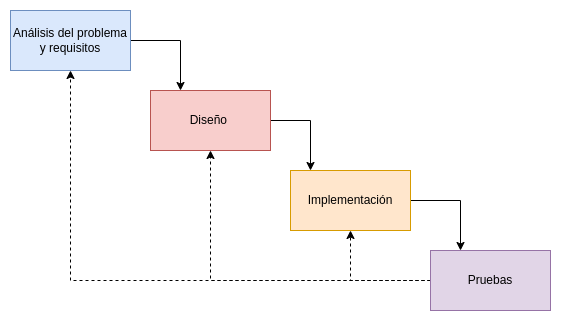
\includegraphics[width=0.8\textwidth]{img/disenio_cascada.png}
        \caption{Diseño en cascada retroalimentado empleado.}
        \label{Fig::Ciclo de vida}
    \end{figure}

    \medskip

    \noindent Las etapas que se seguirán serán las siguientes:

    \begin{enumerate}
        \item \textbf{Análisis del problema y requisitos}: En esta tapa se profundizará sobre el contexto y la importancia del problema a resolver y se llevarán a cabo reuniones con los tutores del trabajo para aclarar los requisitos y objetivos concreto del software a desarrollar. 
        \item \textbf{Diseño}: En nuestro caso, en esta etapa se realizarán dos tareas: 
        
        En primer lugar se diseñará el estudio de la base de datos que emplearemos así como las transformaciones que deban sufrir los datos para poder ser empleados por el software que emplearemos en la fase de experimentación. 

        En segundo lugar se diseñarán los experimentos a realizar así como las técnicas que se aplicarán, las métricas y los protocolos de validación que se usarán.

        \item \textbf{Implementación}: Se implementan todas las técnicas diseñadas en la etapa anterior.
        \item \textbf{Experimentación}: Se ponen en práctica todos los experimentos diseñados de forma teórica y se obtienen resultados. En función de estos se valora una vuelta atrás en el ciclo de vida del software para realizar modificaciones en el software.
    \end{enumerate}
    
    \medskip

    \noindent Debido a la alta carga de trabajo durante el curso, desde un comienzo, el desarrollo del trabajo se planificó pensando en su defensa para la convocatoria extraordinaria de Septiembre o para la convocatoria especial de Noviembre. Por ello, la planificación original por meses se puede observar en la \autoref{Fig::Planificacion original}.


    \begin{figure}[!h]
        \centering
        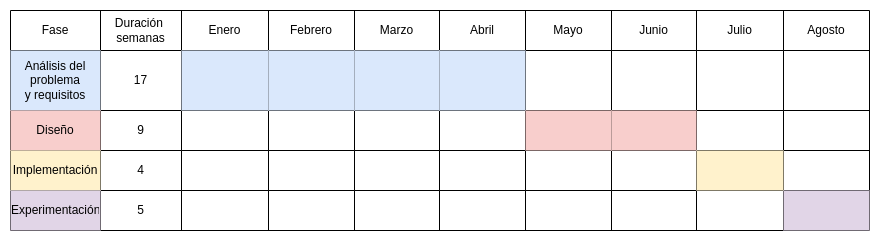
\includegraphics[width=0.8\textwidth]{img/plan_provisional.png}
        \caption{Planificación original.}
        \label{Fig::Planificacion original}
    \end{figure}

    \medskip

    \noindent Dentro de la semana computan únicamente los días de Lunes a Viernes. Resalta a la vista la gran cantidad de semanas invertidas en las primeras dos etapas con respecto a las invertidas en las dos últimas. El principal motivo para repartir el tiempo de esta manera es que durante el curso se calculó que sería imposible dedicar al trabajo más de \textbf{cuatro horas por semana}. En cambio, una vez terminado el curso se previó dedicar una media de \textbf{seis horas diarias al trabajo}. Es por ello que a pesar de la gran diferencia de semanas, si miramos las horas obtenemos:
    
    \begin{itemize}
        \item Para la primera fase se invirtieron un total de \textbf{68 horas}.
        \item Para la segunda fase un total de \textbf{36 horas}.
        \item Para la tercera y cuarta fase se invirtieron un total de \textbf{120 horas} para cada una.
        \item En total el tiempo estimado de desarrollo del proyecto fue de \textbf{344 horas}.
    \end{itemize}
        
    \noindent No obstante, esta estimación resultó ser muy ajustada para completar el trabajo, lo que ocasionó que se retrasara la entrega del mismo a Noviembre, es por ello que el plan definitivo del proyecto se puede ver en la \autoref{Fig::Planificacion final}. Aquí se puede ver cómo desde Septiembre, a causa de los resultados obtenidos en la experimentación se vuelve atrás en el ciclo de vida del software a la parte de análisis del problema y requisitos para consultar a los tutores con los resultados obtenidos y modeificar el resto de etapas sucesivas. El tiempo invertido por día en esta segunda fase fue de \textbf{4 horas} diarias. Lo que incrementa el tiempo total invertido a:

    \begin{itemize}
        \item \textbf{148 horas} para la primera fase.
        \item Para la segunda fase un total de \textbf{76 horas}.
        \item Para la tercera y cuarta fase se invirtieron un total de \textbf{160 horas} para cada una.
        \item En total el tiempo estimado de desarrollo del proyecto fue de \textbf{544 horas}.
    \end{itemize}

    \begin{figure}[!h]
        \centering
        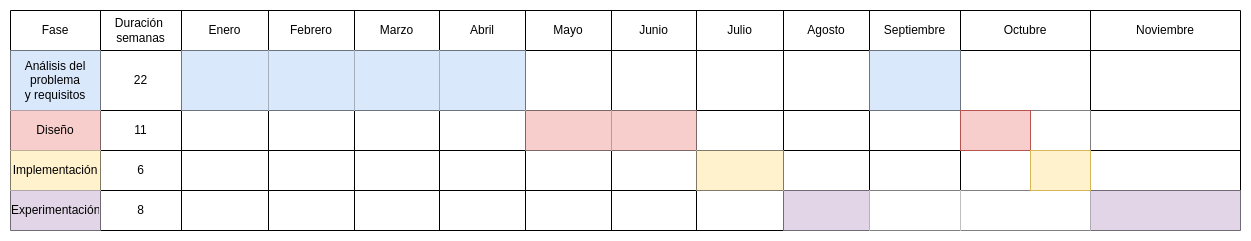
\includegraphics[width=0.8\textwidth]{img/plan_definitivo.png}
        \caption{Planificación original.}
        \label{Fig::Planificacion final}
    \end{figure}

    \medskip

    \noindent Como consecuencia, en un principio se preveía usar un total de \textbf{344} horas para finalizar el trabajo, pero finalmente hicieron falta \textbf{544} horas, de esta forma, si se supone que un Investigador en una empresa de base tecnológica es de 35€/hora, a partir de los resultados obtenidos, el trabajo tenía un presupuesto inicial de \textbf{12.040 €} que finalmente fue ampliado a \textbf{19.040 €}.
    
\endinput
%------------------------------------------------------------------------------------
% FIN DEL CAPÍTULO. 
%------------------------------------------------------------------------------------




\chapter{Fundamentos Teóricos}

En esta sección vamos a introducir cuales serían los conceptos teóricos más importantes que conviene tener presentes para la correcta comprensión del trabajo y sus resultados.

\section{Aprendizaje Automático}
    \noindent Actualmente la \textbf{Inteligencia Artificial} (IA) es una rama de la informática muy popular y de gran importancia que pretende dotar a los ordenadores de una manera de razonar o solucionar problemas inteligente. En este contexto, la IA ha explorado diversos métodos para conseguir este propósito como son el estudio de Metaheurísticas, la Ingeniería del Conocimiento y más recientemente el conocido \textbf{Aprendizaje Automático} (AA). 
    
    \medskip

    \noindent Los métodos que empleamos en este trabajo pretenecen a la rama del AA, y por lo tanto es importante comenzar definiendo qué es este concepto. Para ello, disponemos de diversas definiciones proporcionadas por distintos autores: 

    \medskip

    \noindent La primera y más clásica nos la proporciona Arthur Samuel en 1959, en la cual define el AA como \textbf{el campo de estudio que da a los ordenadores la capacidad de aprender sin ser programados explícitamente}. Esta definición es muy general, pero nos permite hacernos una idea de lo que pretende conseguir este campo de estudio, que es dotar a los ordenadores de la capacidad de \entrecomillado{aprender}, generalmente a partir de una base de datos, con la idea de poder usar este conocimiento adquirido durante el aprendizaje para resolver casos nuevos del problema que la máquina no conozca previamente.
    
    \medskip

    \noindent Una definición un poco más reciente de Tom Mitchell (1998) nos dice que: \textbf{Un programa de ordenador se dice que aprende de la experiencia E respecto de alguna tarea T y alguna medida de rendimiento P, si su rendimiento en T, medido por P, mejora con la experiencia E}. Esta segunda definición nos permite identificar los elementos necesarios para poder resolver un problema mediante técnicas de AA. Así, en primer lugar necesitamos una tarea (T) que queremos resolver con ayuda de un ordenador, una experiencia (E) en esa tarea, que generalmente es una base de datos asociada al problema, y una medida de rendimiento (P) que generalmente se asocia con una función objetivo que se pretende minimizar/maximizar.

    \medskip

    \noindent Tradicionalmente, los algoritmos de AA se dividen en dos conjuntos:

    \begin{itemize}
        \item Aprendizaje Supervisado.
        \item Aprendizaje no Supervisado.
    \end{itemize}

    \medskip 
    
    \noindent No obstante, han aparecido otras técnicas más recientes como el Aprendizaje por Refuezo que son muy interesantes y usadas actualmente, pero no vamos a profindizar en ellas pues no son necesarias para el trabajo que nos ocupa.

    \subsection{Aprendizaje Supervisado}
        \noindent Los algoritmos de AA que se emplean en este conjunto se caracterizan porque disponen de una base de datos \textbf{etiquetados} de manera que para cada dato $x$ conocemos su etiqueta asociada $y$, y nuestro objetivo sería tratar de conocer la función $f$ que los relaciona, de manera que $f(x)=y$.

        \medskip

        \noindent Dentro de este grupo podemos encontrar problemas de \textbf{regresión} y de \textbf{clasificación}.

        \subsubsection{Regresión}
            \noindent En los problemas de regresión se pretende obtener la función $f$ que asocia correctamente a cada dato su etiqueta: 
            \begin{equation}
                f(x)=y \; \; con \; \; x\in \mathbb{R}^m \; \; y \in \mathbb{R}^n
            \end{equation}
            
            \noindent Generalmente, obtener la función $f$ exacta es complicado, por lo que se pretende aproximar mediante una función $f'$ que elegimos y que entrenaremos a partir de los datos etiquetados que se nos proporcionan. Volviendo a la definición de Tom Mitchell, en este tipo de problemas tendríamos que 
            
            \begin{itemize}
                \item T= regresión (aproximar $f$)
                \item E= El conjunto de datos $X$ etiquetados que se proporcionan para entrenar el modelo $f'$.
                \item P= función de coste asociada (generalmente se emplea el error cuadrático medio) que nos mide lo \entrecomillado{bien} que nuestra función $f'$ aproxima a $f$.
            \end{itemize}
            
            \medskip 

            \noindent Por ejemplo el si intentamos predecir $f$ mediante un modelo lineal: 

            \begin{equation}
                f'(x)= \alpha^T x \; \; x,\alpha \in \mathbb{R}^m
            \end{equation}

            \noindent Disponemos de un conjunto de $N$ datos 
            
            \begin{equation}
                X= \lbrace x_1, x_2 , \ldots , x_N \rbrace \; \; x_i \in \mathbb{R}^m
            \end{equation}

            \noindent Además de un conjunto de etiquetas

            \begin{equation}
                Y= \lbrace y_1, y_2 , \ldots , y_N \rbrace \; \; y_i \in \mathbb{R}^n
            \end{equation}

            \noindent Y usamos como medida de error el error cuadrático medio: 

            \begin{equation}
               J(\alpha)= \frac{1}{N} \sum_{i=1}^{N}(f'(x_i) - f(x_i))^2 = \frac{1}{N} \sum_{i=1}^{N}(y_i' - y_i)^2
            \end{equation}

            \noindent Dónde $y_i'$ es la etiqueta predicha por $f'$ para $x_i$.

            \medskip

            \noindent Nuestro objetivo sería encontrar el vector de pesos $\alpha$ que minimice la función de coste $J$ y para ello utilizamos los datos de entrenamiento $X$.
            
        \subsubsection{clasificación}
            \noindent Por otro lado tenemos los problemas de clasificación, en los datos se encuentran agrupados en clases y se pretende clasificar cada dato de entrada en la clase correcta. Los casos más sencillos de este problema son los de \textbf{clasificación binaria}, y en ellos se pretende agrupar los datos en dos posibles clases que suelen codificarse como $0$ y $1$.

    \subsection{Aprendizaje no Supervisado}
            \noindent El aprendizaje no supervisado se caracteriza porque los datos que se proporcionan no están etiquetados, y no se busca una salida concreta, sino que se pretende analizar las características de nuestro conjunto de datos. 

            Así, por ejemplo, tareas que pueden resolverse con esta técnica pueden ser la agrupación de clientes de cierta compañía en distintas clases según sus características.
            
    \subsection{Nuestro Problema}
        \noindent En nuestro problema, los frameworks de los que disponemos resuelven problemas de aprendizaje supervisado y no supervisado. 
        
        \medskip
        
        \noindent Por ejemplo vamos a intentar predecir los landmarks cefalométricos para una cierta imagen de entrada, lo que nos llevaría a un problema típico de aprendizaje supervisado en el que pretendemos a partir de la imagen de entrada conocer la función que nos proporciona la salida correcta (la imagen con los landmarks marcados correctametne).

        \medskip

        \noindent Por otro lado, uno de nuestros frameworks tiene una etapa de entrenamiento previa al problema de los landmarks en la cual mediante conjuntos de datos de imágenes sin etiquetar de rostros humanos, se pretende reconstruir imágenes preservando al máximo posible la estructura de la cara. Esto, como podemos ver, es un problema típico de aprendizaje no supervisado, porque no se busca obtener una etiqueta para cada imagen, sino analizar la estructura de los distintos elementos de los datos de entrada para ser capaces de reconstruirlos preservando su estructura.

\section{Visión por Computador}


\section{Deep Learning}

\section{Redes Neuronales Convolucionales Profundas}

\section{Tratamiento de imágenes 2D y técnicas de few-shot learning}

\endinput
%------------------------------------------------------------------------------------
% FIN DEL CAPÍTULO. 
%------------------------------------------------------------------------------------



\chapter{Estado del Arte}

    \noindent En esta sección nuestro objetivo será realizar una investigación por la literatura y los artículos publicados relacionados con el reconocimiento automático de landmarks cefalométricos en tareas de antropología forense para finalmente justificar nuestra elección en el presente trabajo para tratar de resolver el problema. Para ello utilizaremos la base de datos \textit{Scopus} para realizar la búsqueda y consulta de artículos científico publicados.

    \section{Localización de landmarks cefalométricos en imágenes}

        \noindent Para hacernos una primera idea del estado actual del problema de reconocimiento de landmarks faciales en imágenes realizamos una primera consulta en \textit{SCOPUS} \autoref{fig:SCOPUS1} con la siguiente \textit{keyword} restringiendo los artículos a aquellos relacionados con la informática:
        
        \begin{verbatim}
            TITLE-ABS-KEY ( 
                facial  
                AND  
                ( landmarks  OR  keypoints )  
                AND  
                detection 
                )  
                AND  
                ( LIMIT-TO ( SUBJAREA ,  "COMP" ) )
        \end{verbatim}
        
        \medskip
        
        \noindent Como podemos observar, actualmente existe una tendencia creciente en la publicación de papers relacionados con este tema, en particular esta tendencia comienza en los años en que surge el Deep Learning y las CNN comienzan a utilizarse en visión por computador para el tratamiento de imágenes. 

        \begin{figure}[htpb]
            \centering
            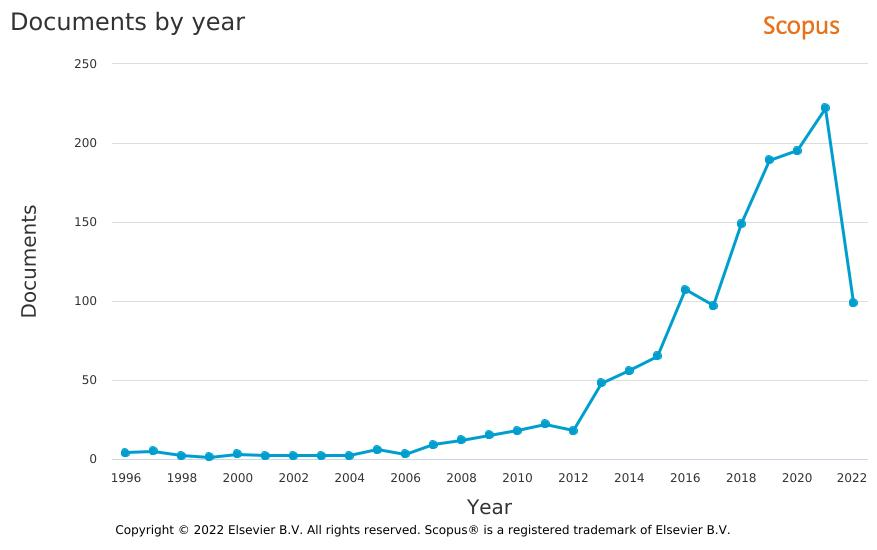
\includegraphics[width=0.6\textwidth]{img/Scopus_1.jpg}
            \caption{Gráfica de publicaciones por año obtenida con la primera \textit{keyword} el $14$ de Julio de $2022$. Destaca el notable incremento de papers a partir de 2012, año en que aparece la red AlexNet y comienza a ganar popularidad el Deep Learning en el tratamiento de imágenes.}
            \label{fig:SCOPUS1}
        \end{figure}

        \medskip

        \noindent Sin embargo los artículos que se han encontrado en \autoref{fig:SCOPUS1} no guardan una relación muy estrecha con el problema de deteción de landmarks cefalométricos en problemas de antropología forense, por ello para descubrir el estado del arte en este campo nos vemos obligados a realizar otra consulta en scopus un poco más concreta y que nos permita conocer mejor las publicaciones más relevantes en este campo en los últimos años descartando los que no sean artículos relacionados con informática. La consulta que realizamos es la siguiente: 

        \begin{verbatim}
            TITLE-ABS-KEY ( 
                ( 
                    ( anthropology  OR  ( anthropology  AND  forensic ) )  
                    AND  
                    ( cephalometric  AND  ( landmarks  OR  keypoints ) ) 
                )  
                
                OR  
                
                ( 
                    ( anthropology  OR  ( anthropology  AND  forensic ) )  
                    AND  
                    ( facial  AND  ( landmarks  OR  keypoints ) ) 
                ) 
                )  
                AND  
                ( LIMIT-TO ( SUBJAREA ,  "COMP" ) )
        \end{verbatim}

        \medskip

        \noindent Con la búsqueda anterior se obtienen un total de $14$ artículos, algo que nos confirma que es un área de investigación en la que apenas hay bibliografía o artículos. Podemos ver un gráfico de resultados de la búsqueda en \autoref{fig:SCOPUS2}.

        \begin{figure}[htpb]
            \centering
            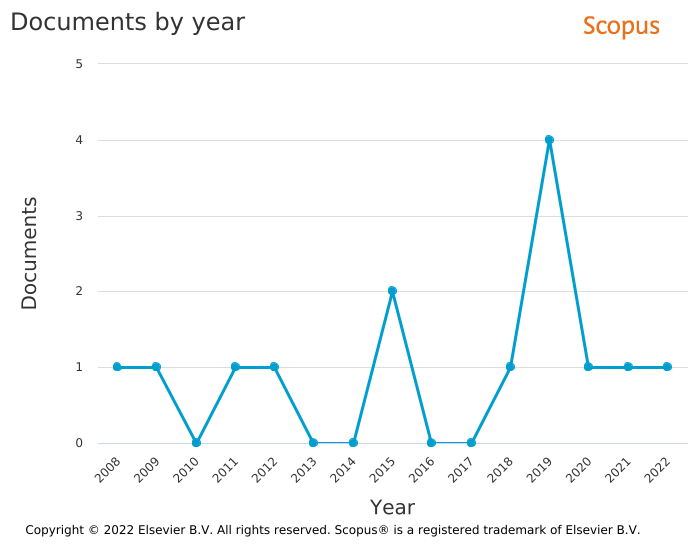
\includegraphics[width=0.6\textwidth]{img/Scopus_2.png}
            \caption{Gráfica de publicaciones por año obtenida con la segunda \textit{keyword} el $14$ de Julio de $2022$. La tendencia es a un artículo por año, aunque destaca el pico de tres artículos en 2015 y el de cuatro en 2019.}
            \label{fig:SCOPUS2}
        \end{figure}

        \subsection{Evolución en la identificación forense de landmarks cefalométricos}
            
            \noindent Como hemos visto antes, la literatura existente es prácticamente nula, además de los catorce artículos obtenidos con la búsqueda anterior, la mayoría no se centran en el reconocimiento de landmarks cefalométricos en imágenes de rostros, hay artículos que se centran en la superposición craneofacial y otros basados en la identificación de landmarks en cráneos. Por lo tanto, de los catorce artículos vamos a destacar los siguientes por la relación directa con nuestro problema ordenados de mayor a menor antigüedad: 

            \subsubsection{Two different approaches to handle landmark location uncertainty in skull-face overlay: coevolution vs fuzzy landmarks}
                \noindent Se trata de un artículo pulicado en $2011$ por Óscar Ibáñez et al \cite{ibanez2011two} en el cual abordan el problema de la superposición craneofacial diseñando un nuevo algoritmo basado en coevolución capaz de reducir el proceso de \textit{Skull-face overlay} (SFO) que tradicionalmente podía llegar a tardar unas 24 horas y comparándolo con un algoritmo ya existente basado en landmarks imprecisos en el cual el antropólogo forense marca regiones de la imagen en las que se encuentra cada landmark (esta tarea no está automatizada en este algoritmo). Aunque no guarda una relación directa con el problema, el algoritmo propuesto realiza una identificación de landmarks cefalométricos en imágenes, por lo que hemos decidido incluirlo en el estudio.

                \medskip

                \noindent Durante el proceso de SFO se dispone de un modelo $3$D de un cráneo y de una imagen, de manera que se considera exitoso el proceso cuando se coloca el cráneo en la misma posición en que aparece en la imagen. Durante este proceso se deben tener en cuenta factores como la edad de la persona, el peso o las expresiones faciales, que añaden un grado más de dificultad a la tarea.

                \medskip

                \noindent Generalmente se dispone de un conjunto de landmarks marcados tanto en la imagen como en el cráneo, y la tarea del SFO se reduce en calcular la transformación que permite llevar los landmarks del cráneo a ocupar la misma posición que en la imagen.

                \medskip

                \noindent La alternativa al algoritmo basado en landmarks imprecisos es un algorimto coevolutivo en el cual el valor de la función de fitness de cada elemento depende de la de él mismo y otros individuos que pueden interaccionar de forma cooperativa o conflictiva. Adaptado al problema de SFO tendríamos dos poblaciones: el conjunto de parámetros que definen la transformación que se aplica al modelo $3$D del cráneo y por otro lado las localizaciones de los landmarks cefalométricos. Ambas poblaciones colaboran para encontrar la mejor transformación posible y solucionar el SFO.

                \medskip

                \noindent En el experimento se disponía de seis procesos distintos de SFO correspondientes a tres casos reales proporcionados por el laboratorio de Antropología Física de la Universidad de Granada en colaboración con la policía científica. Se disponía así de tres modelos $3$D de cráneos pertenecientes a personas desaparecidas junto con un dataset de seis imágenes. Las imágenes, a pesar de ser pocas, presentan una gran variedad en iluminación, posición (hay imágenes frontales y en $3/4$) y con problemas de oclusión en algunos casos para los landmarks a causa del cabello. Por otro lado la calidad de las imágenes es muy variada, habiendo imágenes de gran resolución y otras de baja calidad. Finalmente se disponen cuatro imágenes para el caso de estudio $3$ y una única imagen para el caso de estudio $1$ y $2$.

                \medskip
                

                \noindent En el experimento, el algoritmo empleado para la técnica de encontrar landmarks imprecisos es CMA-ES, y se comparó con el algoritmo coevolutivo desarrollado. Las conclusiones fueron que el nuevo algoritmo reducía considerablemente los tiempos de ejecución del algoritmo basado en landmarks imprecisos y que realizaba una Localización de landmarks cefalométricos apropiada. 
                
                \medskip

                \noindent Por lo tanto podemos considerar este primer algoritmo coevolutivo como la primera aproximación a nuestro problema de detección automática de landmarks. A pesar de lo pobre que es el conjunto de datos de entrenamiento, se emplean imágenes que se encuentran en nuestro dataset y con diversas posturas y resolución de imagen. No obstante, la parte de detección de landmarks no es la principal de este artículo, pues aunque es una consecuencia del algoritmo que se desarrolla, se pretende realizar con el mayor éxito posible la fase SFO.

            \subsubsection{Automatic craniofacial anthropometry landmarks detection and measurements for the orbital region}
                \noindent Se trata de un artículo publicado en $2014$ por Salina Mohd et al \cite{asi2014automatic} en el que se pretende diseñar un método para calcular en una imagen de los ojos de un sujeto el \textit{endocathion} y el \textit{exocanthion} basado en el uso de un clasificador entrenado sobre filtros de Haar usados para la identificación de caras por Viola-Jones.

                \medskip

                \noindent Lo primero que llama la atención del artículo es que tan solo pretende ser capaz de identificar dos landmarks, mientras que en nuestro problema por ejemplo tratamos de predecir la posición de unos treinta (incluyendo en \textit{endocathion} y el \textit{exocanthion}).

                \medskip

                \noindent En segundo lugar, cabe destacar la manera en que se resuelve el problema, pues se hace uso de un clasificador en cascada basado en filtros de tipo Haar como se pueden ver en la \autoref{fig:asi2014}. Este es un método tradicional de la visión por computador en el que mediante el paso y convolución de este tipo de filtros por la imagen se obtiene información de esta relativa a los contornos. No obstante se trata de un método que ya se ha visto superado por otras técnicas más recientes de deep learning.

                \begin{figure}[!h]
                    \centering
                    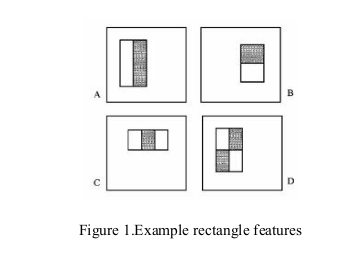
\includegraphics[width=0.8\textwidth]{img/caracteristicas_haar.png}
                    \caption{Ejemplo de filtros empleados en el artículo \cite{asi2014automatic} de donde procede esta imagen.}
                    \label{fig:asi2014}
                \end{figure}

                \medskip

                \noindent Por otro lado, el conjunto de datos que se emplea se ha obtenido en entornos controlados con buena iluminación, algo que no guarda relación con nuestro problema pues se trata de imágenes en diversas posturas, iluminación, y resolución.

            \subsubsection{Automated facial landmark detection, comparison and visualization}
                \noindent Se trata de un trabajo realizado en $2015$ por Marek Galvánek et al. \cite{galvanek2015automated} para la detección automática de landmarks en modelos $3D$ de imágenes de personas. 

                \medskip

                \noindent Los landmarks detectados por el modelo son en total $14$ y todos ellos pertenecen también al conjunto de landmarks que se detectan en este trabajo fin de grado.

                \medskip

                \noindent El algoritmo propuesto se basa en la curvatura de la superficie del modelo $3$D y en la simetría del perfil. En primer lugar se alinea el modelo $3$D con el plano horizontal de Frankfort \autoref{fig:Frankfort}, un plano utilizado por los antropólogos forenses para marcar landmarks. En segundo lugar se realiza un estudio de la curvatura del modelo $3$D en la zona de la nariz, boca y ojos. Finalmente con el perfil del modelo y la simetría se rectifican y perfeccionan los landmarks marcados en etapas previas.

                \begin{figure}[!h]
                    \centering
                    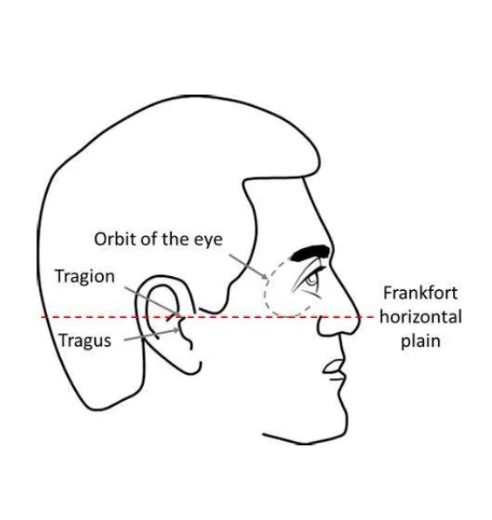
\includegraphics[width=0.5\textwidth]{img/frankfort.png}
                    \caption{Cara alineada con el plano horizontal de Frankfort. Imagen extraida de \url{https://www.slideshare.net/NiharikaSupriya/cephalometrics-landmarkslines-and-planes-93890774
                    }}
                    \label{fig:Frankfort}
                \end{figure}

                \medskip

                \noindent El algoritmo propuesto resulta interesante, aunque no detecta un elevado número de landmarks y se hace de una forma parecida a como un antropólogo forense actuaría. Podemos ver también que es muy preciso en la detección si comparamos los landmarks marcados por el algoritmo con los marcados por un experto manualmente en la \autoref{fig:landmarks_comparativa}.


                \begin{figure}[!h]
                    \centering
                    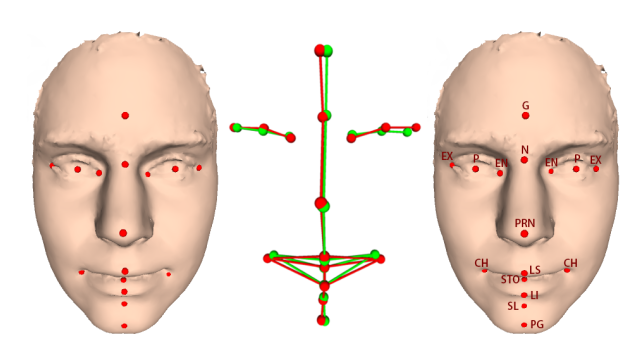
\includegraphics[width=0.8\textwidth]{img/comparativa_landmarks.png}
                    \caption{Comparativa entre los landmarks marcados por el algoritmo (izquierda) y los marcados por un experto (derecha). Imagen extraida de \cite{galvanek2015automated}.}
                    \label{fig:landmarks_comparativa}
                \end{figure}

                \medskip

                \noindent En este trabajo, comenzamos a ver ya un problema similar al nuestro, la detección automática de landmarks cefalométricos con un mayor número de landmarks ($14$ frente a los $2$ del estudio anterior). Aunque se realiza sobte modelos $3$D de caras que evitan problemas de oclusión, mala iluminación o resolución.

            \subsubsection{Automatic cephalometric landmarks detection on frontal faces: An approach based on supervised learning techniques}

                \noindent El siguiente artículo es de $2019$ y fue realizado por Lucas Faria et al. Pretende desarrollar un algoritmo para el reconocimiento automático de landmarks cefalométricos en imágenes frontales a partir de técnicas de visión por computador y de métodos de aprendizaje supervisado \cite{porto2019automatic}.

                \medskip

                \noindent El algoritmo tiene tres componentes:

                \begin{itemize}
                    \item En la primera fase se realiza un pre-procesamiento de las imágenes para resaltar sus caracteristicas faciales. 
                    \item En la segunda fase se aplica la cascada de filtros de Haar de Viola-Jones para identificar las regiones de interés de la imagen: ojos, nariz, boca.
                    \item Finalmente se aplica el algoritmo de machine learning supervisado a cada una de las regiones anteriores. Creando un detector automático de landmarks para cada región.
                \end{itemize}

                \medskip

                \noindent Por otro lado el conjunto de entrenamiento es de $1000$ individuos de los cuales se tomaron fotografías frontales en las mismas condiciones de iluminación y de distancia a la cámara, por lo que no presenta las mismas complicaciones que el dataset del que disponemos. 

                \medskip

                \noindent Destaca este artículo por ser el primero en el cual comienzan a usarse técnicas de aprendizaje automático para la resolución del problema. Además en las imágenes de entrenamiento fueron marcados 28 landmarks que se emplearon para el entrenamiento, que coinciden con los mismos que tenemos en nuestro problema.

            \subsubsection{The Improved Faster R-CNN for Detecting Small Facial Landmarks on Vietnamese Human Face Based on Clinical Diagnosis}
            
                \noindent Este artículo es el más reciente pues fue publicado en Junio de $2022$ por Ho Nguyen Anh Tuan et al \cite{ImprovedfasterRCNN}. En él se utiliza una versión mejorada de la red faster R-CNN aplicada a la tarea del reconocimiento de landmarks cefalométricos. 

                \medskip

                \noindent Los resultados obtenidos son muy buenos pero como ocurre en la mayoría de trabajos de este tipo, la base de datos usada ha sido de imágenes tomadas de voluntarios en unas mismas condiciones de iluminación frontales y de perfil. 

                \medskip

                \noindent No obstante el trabajo restalta la gran importancia que está teniendo el Deep Learning y las CNN en tareas de reconocimiento de landmarks faciales (usualmente landmarks no biológicos como los que se emplean en tareas de antropología forense), y partiendo de esta base podemos justificar el trabajo que vamos a desarrollar, pues nos proponemos adaptar una red que ya ha sido entrenada para la identificación de landmarks faciales en grandes volúmenes de datos de imágenes en diversas posturas y resolución para la tarea del reconocimiento de landmarks forense.

                \medskip

                \noindent Todos los métodos que se han presentado en esta sección trataban de cumplir con el mismo objetivo, y han ido evolucionando con el paso de los años a la par que la informática, empezando por tratar de aplicar algoritmos coevolutivos, después filtros de Haar y técnicas de visión por computador y finalmente usar CNN de Deep Learning. De esta manera y viendo con perspectiva el estado del arte en el campo, consideramos que la propuesta que presentamos puede traer buenos resultados, pues pretendemos enseñar a un sistema experto en el reconocimiento de landmarks no biológicos a identificar estos otros puntos, lo cual puede suponer un nexo de unión entre las dos líneas de investigación.

        \subsection{Nuestra propuesta}
            \noindent El reconocimiento automático de landmarks faciales es una área de gran importancia en la actualidad en tareas como el reconocimiento de personas y que se está viendo muy desarrollado actualmente por la gran capacidad de las CNN para tareas de procesamiento automático de imágenes. 


            \medskip 

            \noindent La principal diferencia entre este enfoque y el forense explicado en la sección anterior radica en el tipo de landmarks que se utilizan. Los utilizados en antropología forense son landmarks con justificación biológica, a diferencia de los que se emplean en las tareas de reconocimiento facial, que generalmente atienden a puntos de interés de la cara para su correcto reconocimiento y son independientes del cráneo del sujeto. Así pues existen diversas bases de datos empleadas para este cometido con multitud de imágenes etiquetadas, destacamos entre ellas: 

            \begin{itemize}
                \item \textbf{300-W}: Se trata de un dataset compuesto por $3148$ imágenes de entrenamiento y $689$ imágenes de test \textit{in-the-wild}, es decir con multitud de poses, distinta iluminación y expresiones faciales. Está anotada por 51 landmarks o 68 landmarks si contamos el contorno del rostro \cite{300W}. Podemos ver los landmarks en la imagen \autoref{fig:300W}
                
                \begin{figure}[!h]
                    \centering
                    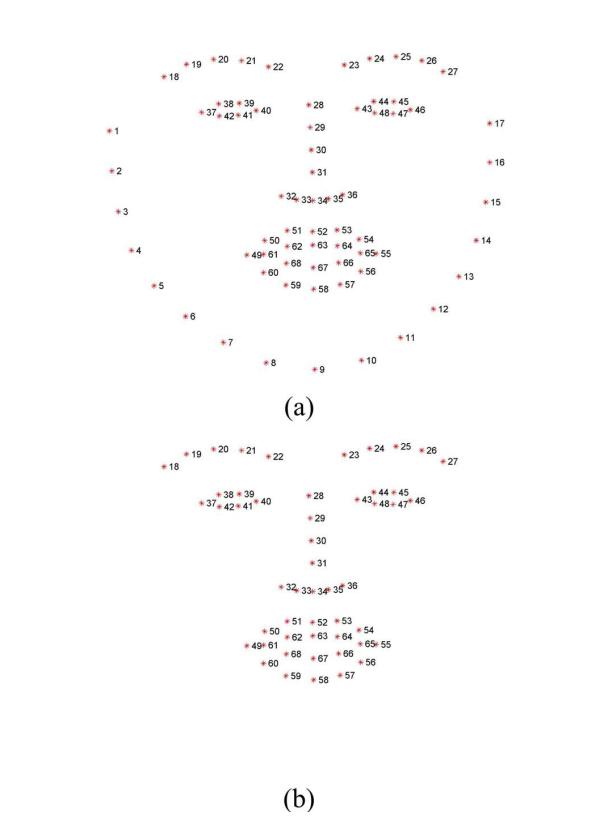
\includegraphics[width=0.8\textwidth]{img/33W.png}
                    \caption{Conjunto de landmarks anotados en el dataset 300W, en la imagen \textit{a} contando el contorno del rostro son un total de 68 landmarks, en la imagen \textit{b} son 51 en total. Imagen extraida de \cite{300W}.}
                    \label{fig:300W}
                \end{figure}
                
                \item \textbf{AFLW}: Se trata de un dataset de $24386$ imágenes \textit{in-the-wild} con un total de 21 landmarks anotados entre las cejas y el mentón, como podemos ver en la imagen \autoref{fig:AFLW}  \cite{AFLW}
                \begin{figure}[!h]
                    \centering
                    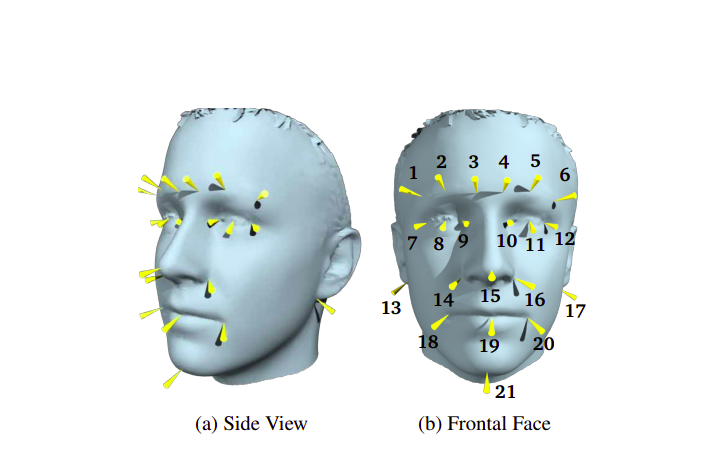
\includegraphics[width=0.8\textwidth]{img/AFLW.png}
                    \caption{Conjunto de landmarks anotados sobre un modelo $3$D que emplea el dataset AFLW. Imagen extraida de \cite{AFLW}.}
                    \label{fig:AFLW}
                \end{figure}
            \end{itemize}
            
            \medskip
            
            \noindent El hecho es que existen actualmente CNN que son capaces de reconocer con un alto grado de precisión estos conjuntos de landmarks marcados por las bases de datos anteriores, lo que nos hace pensar que quizá podría emplearse el conocimiento adquirido por estas redes para reentrenarlas en un proceso de \textit{fine-tuning} sobre una base de datos forense con landmarks anotados por un experto para tratar de resolver el problema de la identificación automática de landmarks. De ahí nace nuestra propuesta, que en cierto modo trata hace como nexo de unión entre las dos vías de investigación.    
\endinput
%------------------------------------------------------------------------------------
% FIN DEL CAPÍTULO. 
%------------------------------------------------------------------------------------


\chapter{Implementación}

\section{Diseño del Sofware}

\noindent El diseño software no se ha orientado a crear un programa funcional para ser empleado por un usuario, sino que tiene como función entrenar los modelos probados y recabar los resultados oportunos del proceso de experimentación. Se ha utilizado el sistema de control de versiones \textit{Git} junto con \textit{GitHub}. En total se han creado dos repositorios:

\begin{enumerate}
    \item Un repositorio con la planificación y elaboración de la memoria junto con los scripts utilziados para el preprocesamiento de los datos: \url{https://github.com/alejbormeg/TFG-LandmarkDetectionAndCNNAnalysis}
    \item Un \textit{fork} a partir del repositorio principal del paper, dónde se han elaborado todas las adaptaciones a nuestro problema: \url{https://github.com/alejbormeg/3FabRec/tree/master}
\end{enumerate}

\medskip

\noindent En primer lugar, se ha programado un \textit{notebook} de Jupyter independiente al proyecto general del framework, en el cual, se realiza el preprocesamiento de los datos, la identificación de las caras y la separación en conjunto de entrenamiento y test. El fichero se denomina \textit{Make-crop-split database.ipynb}.

\medskip

\noindent Por otro lado, en lo que respecta al entrenamiento y diseño de la red, partíamos de un proyecto ya elaborado minuciosamente que se ha tenido que adaptar para aceptar como entrada la nueva base de datos así como alterar ciertas partes de su entrenamiento (para poder hacer el ajuste fino del decoder por ejemplo, realizar técnicas de \textit{cross validation 5-fold}) o introducir nuevos parámetros y funciones para la obtención y manipulación de los datos, y la generación de las gráficas y tablas de resultados que se muestran. Además se tuvieron que alterar las funciones del cálculo de métricas para que tuvieran en cuenta que en todas las imágenes no necesariamente se incluían todos los landmarks, y por lo tanto que solo computasen aquellos presentes en las mismas.

\begin{figure}[!h]
    \centering
    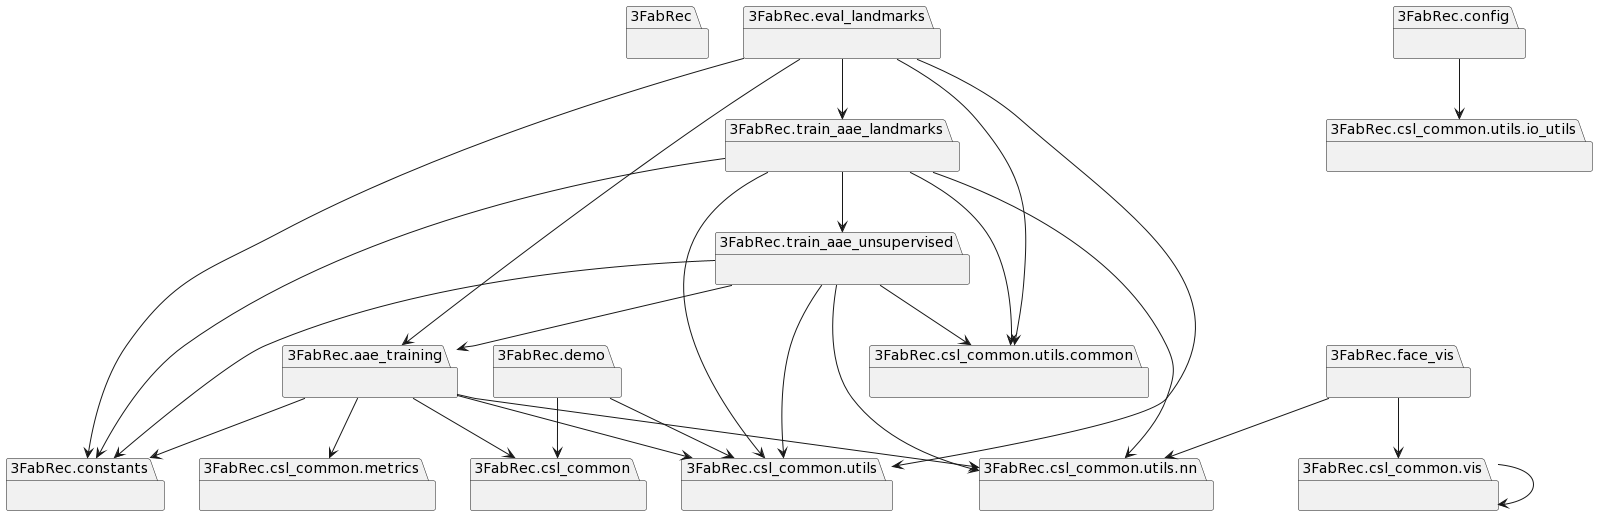
\includegraphics[width=0.99\textwidth]{img/diagrama_paquetes_1.png}
    \caption{Diagrama de paquetes del proyecto generado por \textit{pyreverse}, herramienta incluida en el paquete Pylint}
    \label{fig:Diagrama_paquetes}
\end{figure}

\medskip

\noindent La estructura de paquetes la podemos ver en la \autoref{fig:Diagrama_paquetes}. Los paquetes en color rojo son los que han sido modificados o creados para este trabajo, el resto pertenecen al software original de \cite{browatzki20203fabrec}:

\begin{itemize}
    \item \textcolor{mygreen}{\textbf{3FabRec.eval\_landmarks}}: Se lleva a acabo la evaluación del modelo en el conjunto de test y se extraen las métricas. Se adapta para extraer el \textbf{RMSE} por landmark teniendo en cuenta que cada landmark puede estar no marcado en algunas imágenes.
    \item \textcolor{mygreen}{\textbf{3FabRec.train\_aae\_landmarks}}: Se lleva a cabo todo el proceso del entrenamiento supervisado del marcado de landmarks. Es el fichero que más se ha tenido que modificar, pues hemos cambiado la lógica del entrenamiento con respecto a la del framework original. Los parámetros de ejecución se encuentran en la \autoref{table:Params}.
    \item \textbf{3FabRec.train\_aae\_unsupervised}: En este paquete se lleva a cabo el entrenamiento no supervisado de la red.
    \item Los dos paquetes anteriores, a su vez se combinan en \textbf{3FabRec.aa\_training}, que encapsula toda la lógica del entrenamiento, incluyendo el aprendizaje supervisado y el no supervisado.
    \item El paquete \textbf{3FabRec.landmarks} lleva a cabo todo lo relaitvo a la manipulación de los landmarks, el cálculo de los errores asociados a los mismos, el paso de Heat maps a coordenadas y la inversa, etc... En este fichero se ha tenido que modificar el subpaquete \textcolor{mygreen}{\textbf{3FabRec.lanmarks.lmutils}} y \textcolor{mygreen}{\textbf{3FabRec.landmakrs.lmvis}}. En el caso del primero porque hemos modificado algunas funciones que calculan las métricas de error adaptándolas al problema y en el caso del segundo porque no toda la información que se mostraban en las imágenes de salida era relevante para nuestro estudio, por lo que se han eliminado los datos innecesarios.
    \item El paquete \textbf{3FabRec.constants} contiene variables globales relativas a los conjuntos de datos de entrenamiento, validación y test.
    \item El paquete \textbf{3FabRec.networks} contienen todas las redes que se emplean en la arquitectura de la red. En concreto usaremos \textbf{3FabRec.networks.aae} en la cual se encuentra la estructura general del adversarial autoencoder.
    \item El paquete \textbf{3FabRec.datasets} contiene todos los ficheros relativos a la creación de la clase \textit{Dataset} y \textit{Dataloader} para cada base de datos concreta que se emplea en el framework. Dentro de este paquete se crea el fichero \textcolor{mygreen}{\textbf{3FabRec.datasets.forense\_am}}, que se encarga de la lectura correcta de los datos de entrenamiento de la base de datos proporcionada.
\end{itemize}


\begin{figure}[!h]
    \centering
    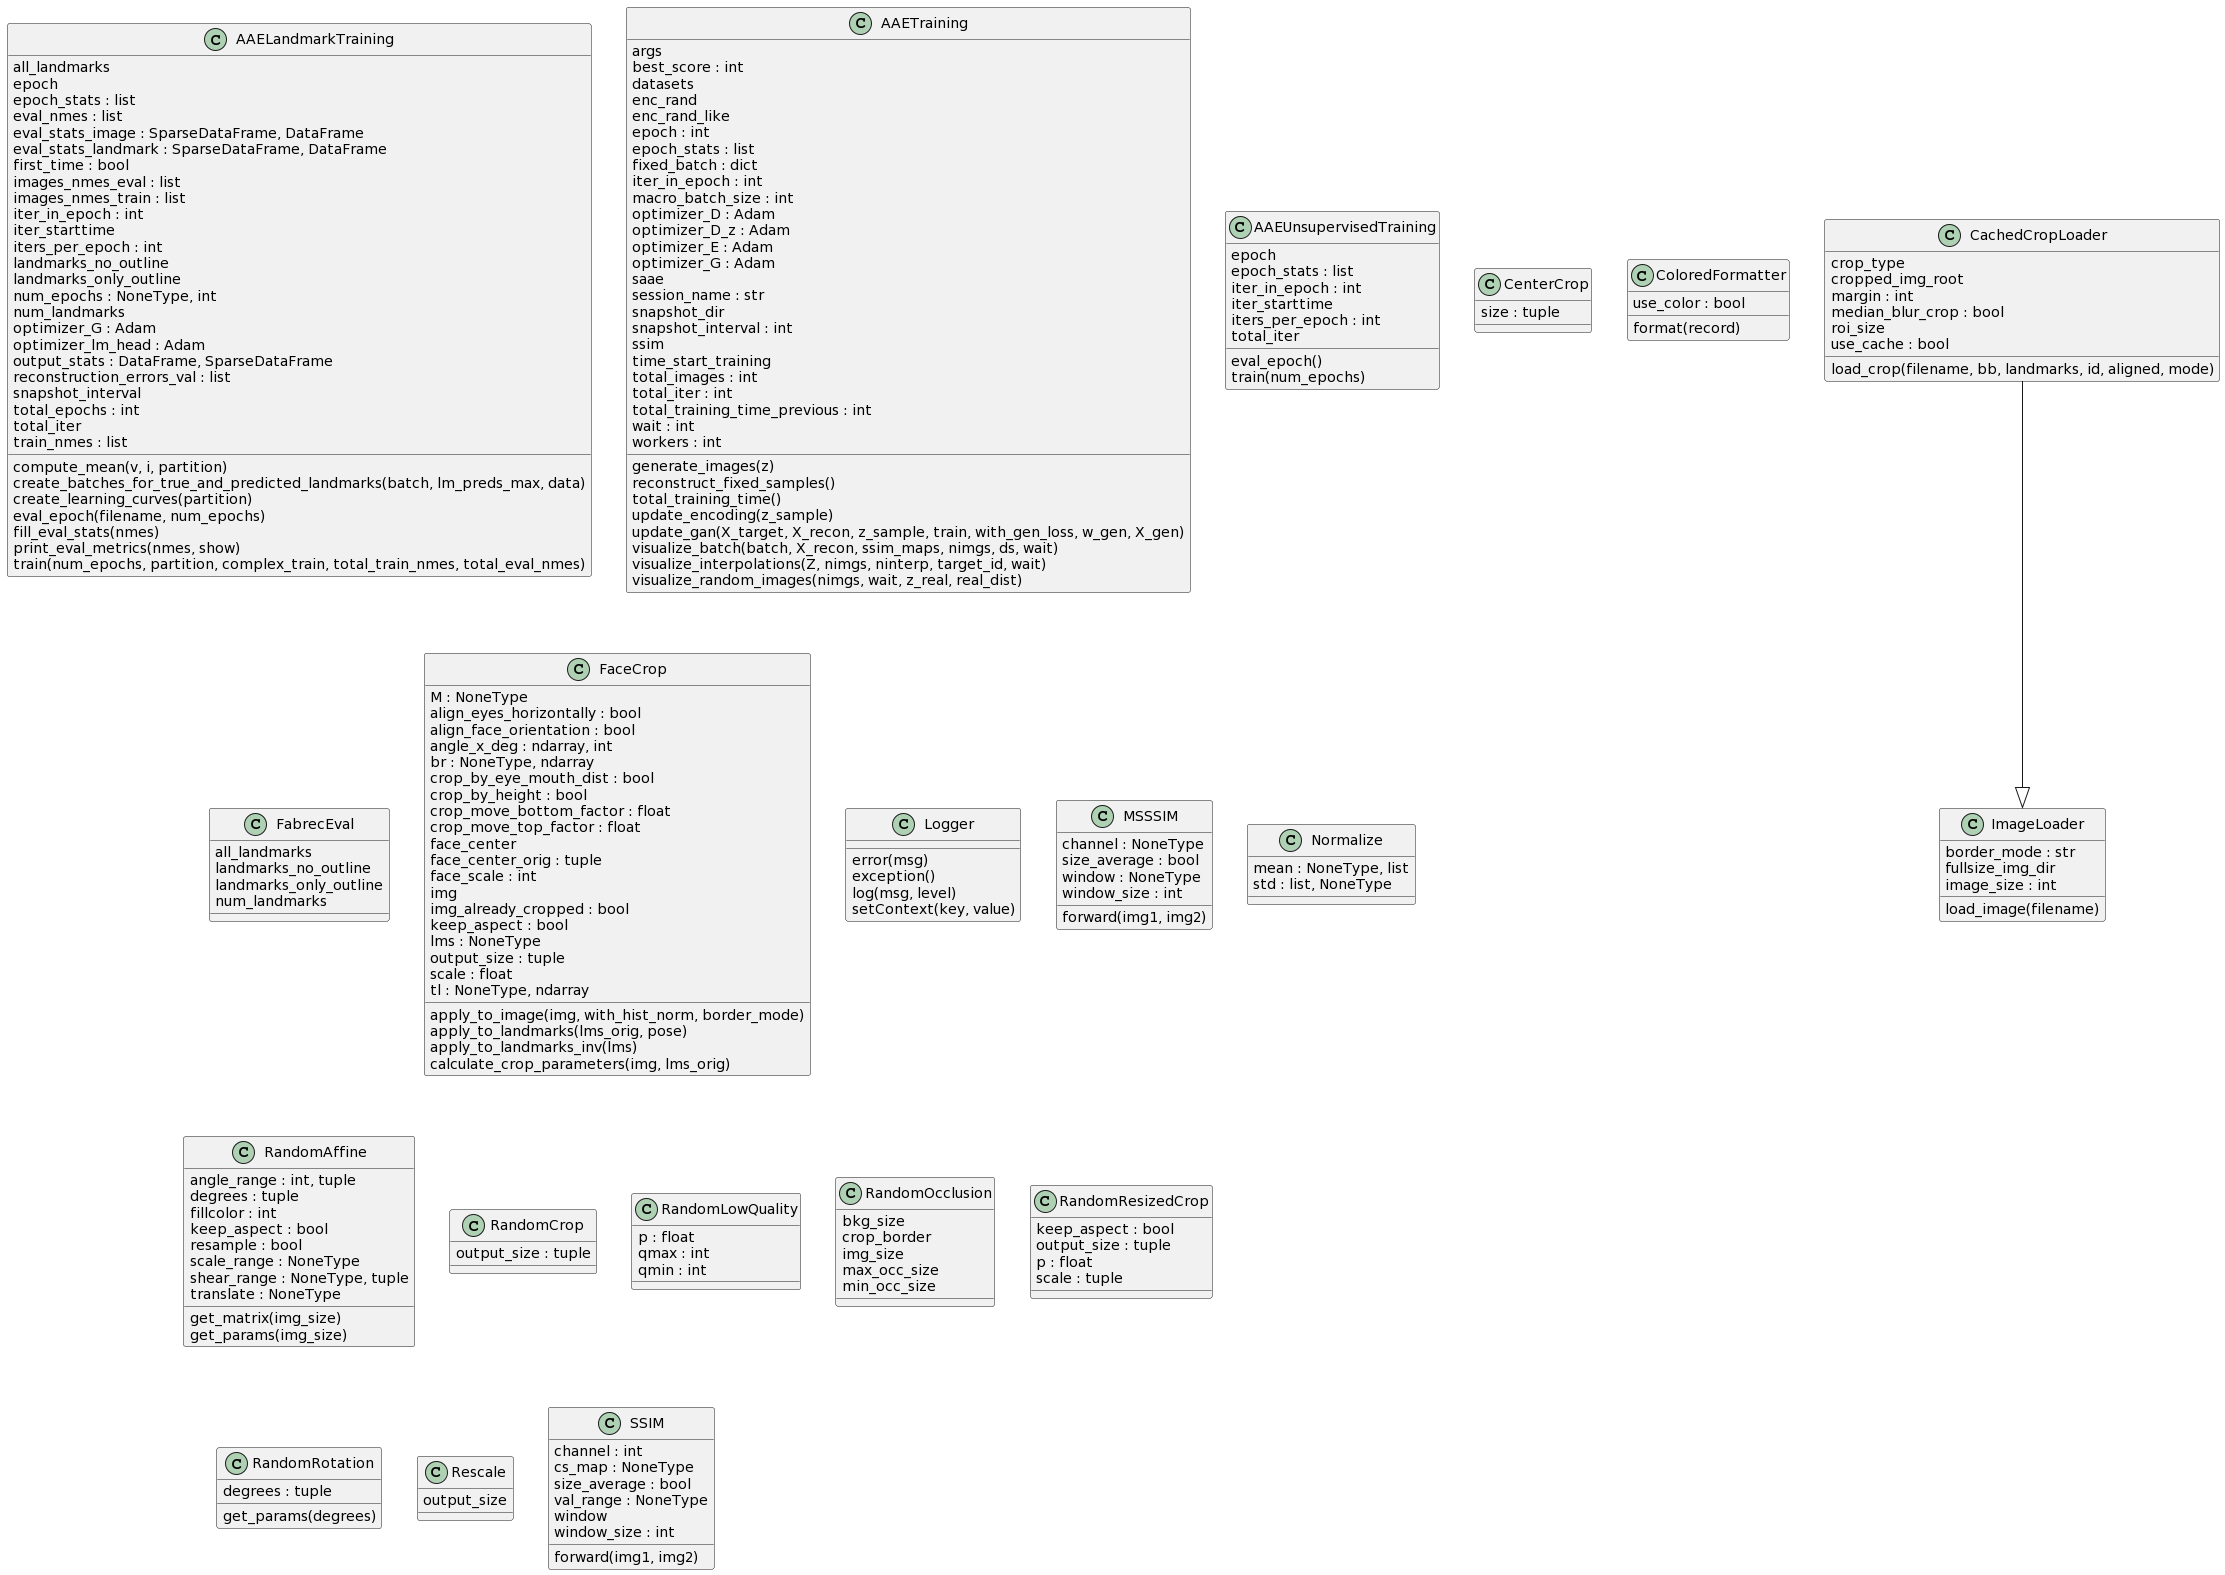
\includegraphics[width=0.99\textwidth]{img/diagrama_clases.png}
    \caption{Diagrama de clases con las principales clases del proyecto.}
    \label{fig:Diagrama_clases}
\end{figure}

\begin{table}[!h]
    \centering
    \caption{Argumentos con los que se ha experimentado en la ejecución del fichero train-aae-landmarks.py}
    \begin{tabular}{|l|l|l|}
    \hline
        Parámetro & Descripción & Valor por defecto \\ \hline
        --train-encoder & Si es True reentrena el encoder & False \\ \hline
        --train-dencoder & Si True reentrena el dencoder & False \\ \hline
        --epochs & Número de épocas que queremos entrenar la red & None \\ \hline
        --batchsize & Tamaño del batchsize para entrenamiento & 50 \\ \hline
        --batchsize-eval & Valor del batchsize para validación & 10 \\ \hline
        --lr & Learning rate para el autoencoder & 0.00002 \\ \hline
        --lr-heatmaps & Learning rate para las ITLs & 0.001 \\ \hline
        --beta1 & Valor de beta 1 para Adam & 0.0 \\ \hline
        --beta2 & Valor de beta 2 para Adam & 0.999 \\ \hline
        --save-freq & Frecuencia de snapshot (en épocas) & 1 \\ \hline
        --dataset & Dataset que se empleará & W300 \\ \hline
        --sigma & Tamaño de los heatmaps & 7 \\ \hline
    \end{tabular}
    \label{table:Params}
\end{table}

\medskip

\noindent Por otro lado, en la \autoref{fig:Diagrama_secuencia} podemos ver el diagrama de secuencia de la ejecución del software 3FabRec para la etapa de entrenamiento y validación y posteriormente para la de evaluación del modelo final. No obstante, remarcamos el hecho de que el software diseñado no tiene como fin su uso por parte de terceros. De ser así, se habría creado una interfaz de usuario amigable en la cual, de manera intuitiva se pudieran elegir las distintas opciones de ejecución.

\newpage

\begin{figure}[!h]
    \centering
    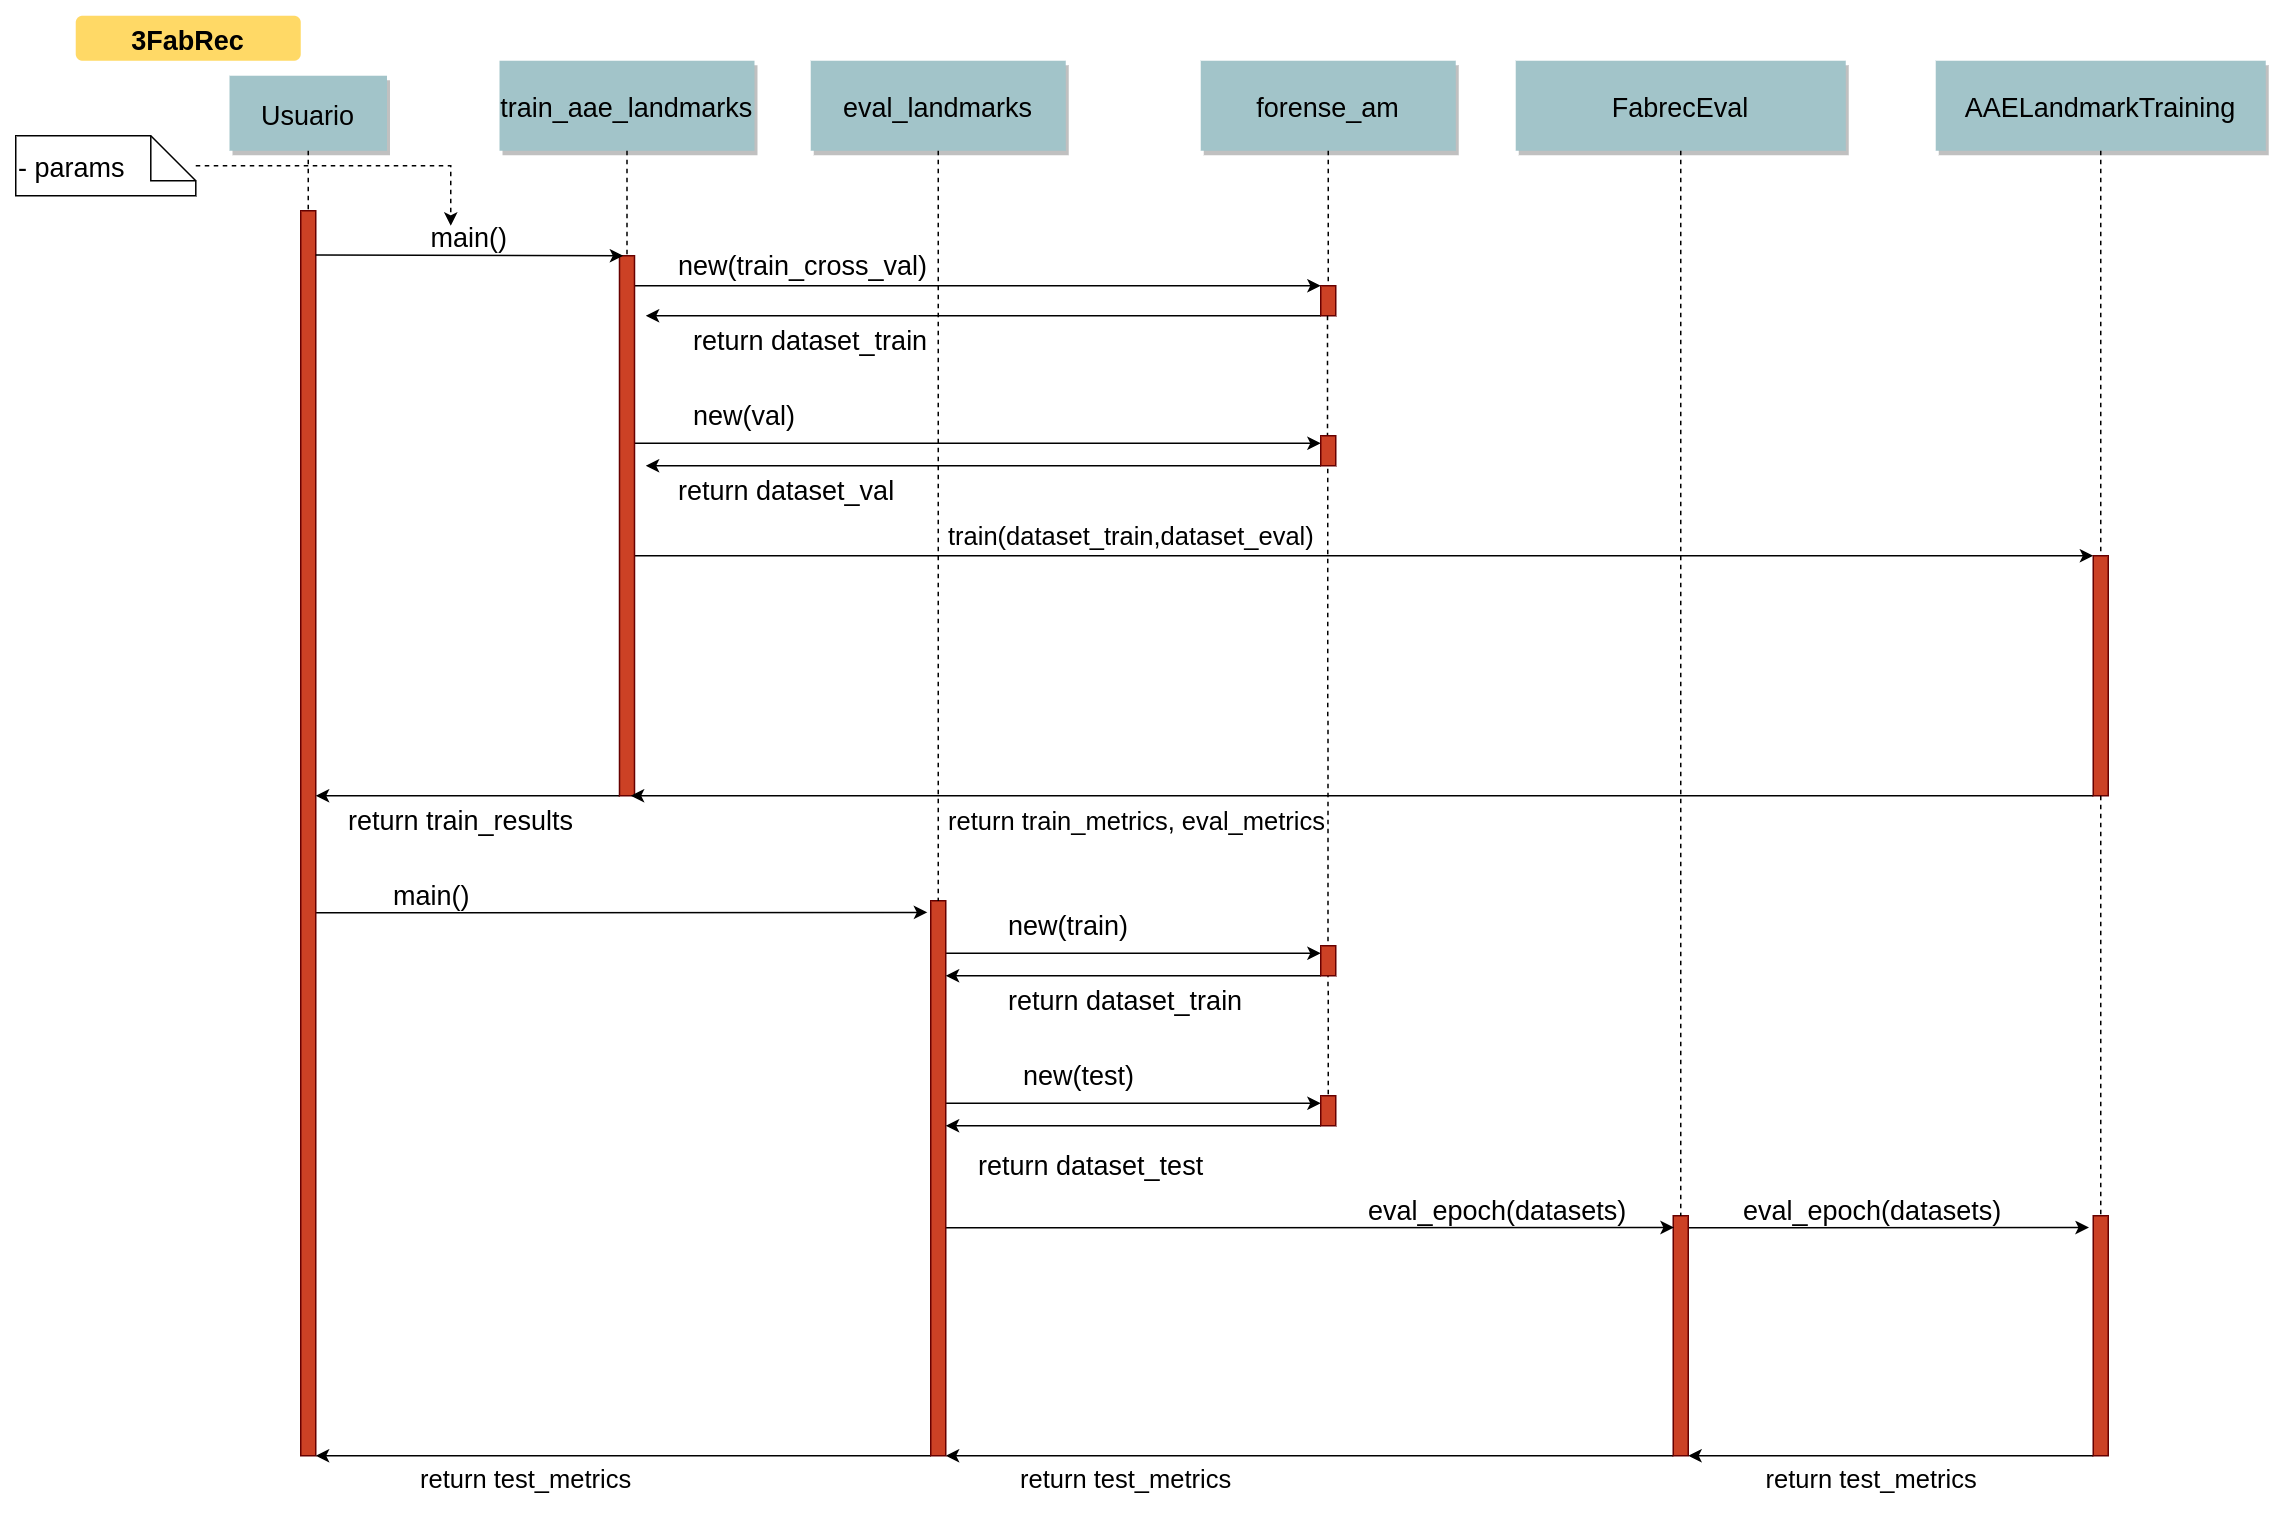
\includegraphics[width=0.99\textwidth]{img/Diagrama_secuencia.png}
    \caption{Diagrama de secuencia del software empleado.}
    \label{fig:Diagrama_secuencia}
\end{figure}

\newpage


\section{Entorno de ejecución}
\noindent Las ejecuciones se han realizado todas en un ordenador portátil \textit{HP Pavilion} con las siguientes características: 

\begin{itemize}
    \item Ubuntu $20.04.5$ LTS $64$ bits.
    \item $8$ GB de RAM
    \item $8$ x Intel® Core™ i$5$-$8300$H CPU @ $2.30$GHz
    \item GPU NVIDIA GeForce GTX $1050$ Mobile
\end{itemize}

\medskip

\noindent Por otro lado, las versiones del software empleado son: 

\begin{itemize}
    \item Python 3.6.13
    \item CUDA 10.1
    \item PyTorch 1.1.0
    \item Numpy 1.17.4
    \item Pandas 0.23.3
    \item Matplotlib 3.3.4
\end{itemize}


\endinput
%------------------------------------------------------------------------------------
% FIN DEL CAPÍTULO. 
%------------------------------------------------------------------------------------


\chapter{Solución propuesta y experimentos realizados}

    \noindent El reconocimiento automático de landmarks faciales es una área de gran importancia en la actualidad en tareas como el reconocimiento de personas y que se está viendo muy desarrollada gracias a las CNN. La principal diferencia entre este enfoque y el forense radica en el tipo de landmarks que se utilizan. Los utilizados en antropología forense son landmarks con justificación biológica. Dichos landmarks se correpsonden con localizaciones concretas del cráneo del ser humano, y los landmarks cefalométricos intentan predecir la posición de estos puntos sobre la piel, a diferencia de los que se emplean en las tareas de reconocimiento facial, que generalmente atienden a puntos de interés de la cara para su correcto reconocimiento y son independientes del cráneo del sujeto. Así pues existen diversas bases de datos empleadas para este cometido con multitud de imágenes etiquetadas, destacamos entre ellas: 

    \begin{itemize}
    \item \textbf{300-W}: Se trata de un dataset compuesto por $3148$ imágenes de entrenamiento y $689$ imágenes de test \textit{in-the-wild}, es decir con multitud de poses, distinta iluminación y expresiones faciales. Está anotada por 51 landmarks o 68 landmarks si contamos el contorno del rostro \cite{300W}. Podemos ver los landmarks en la imagen \autoref{fig:300W}
    
    \begin{figure}[h]
        \centering
        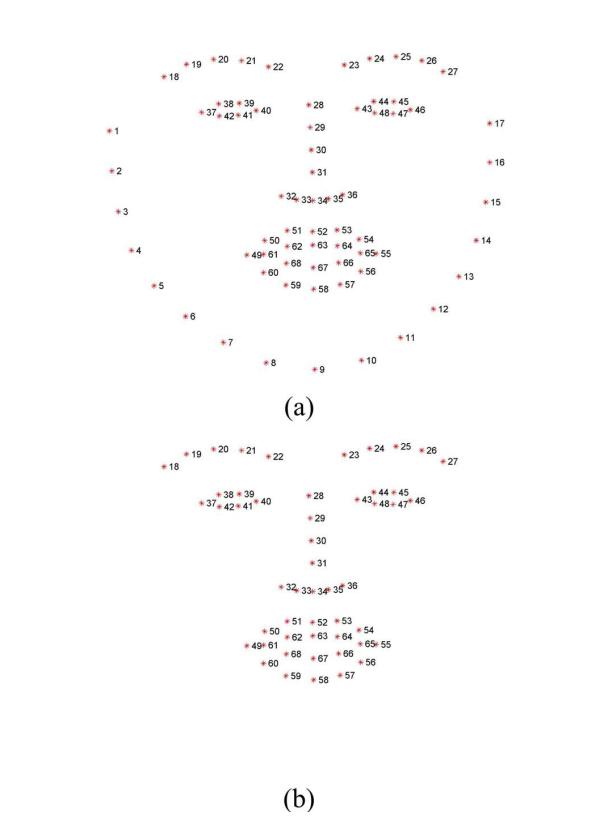
\includegraphics[width=0.5\textwidth]{img/33W.png}
        \caption{Conjunto de landmarks anotados en el dataset 300W, en la imagen \textit{a} contando el contorno del rostro son un total de 68 landmarks, en la imagen \textit{b} son 51 en total. Imagen extraida de \cite{300W}.}
        \label{fig:300W}
    \end{figure}
    
    \item \textbf{AFLW}: Se trata de un dataset de $24386$ imágenes \textit{in-the-wild} con un total de 21 landmarks anotados entre las cejas y el mentón, como podemos ver en la imagen \autoref{fig:AFLW}  \cite{AFLW}
    \begin{figure}[H]
        \centering
        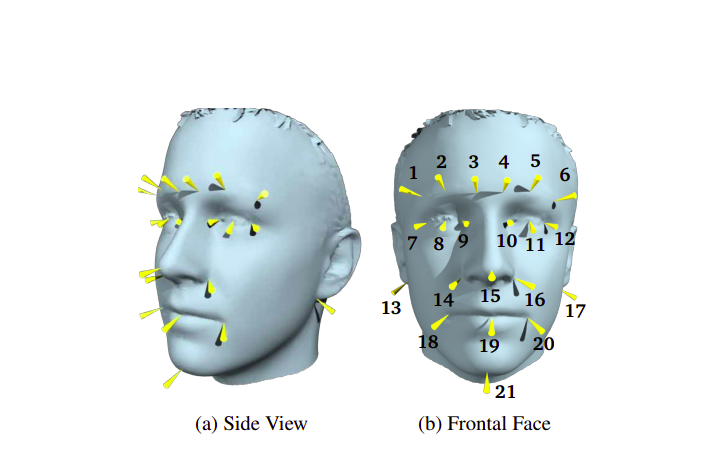
\includegraphics[width=0.8\textwidth]{img/AFLW.png}
        \caption{Conjunto de landmarks anotados sobre un modelo $3$D que emplea el dataset AFLW. Imagen extraida de \cite{AFLW}.}
        \label{fig:AFLW}
    \end{figure}
    \end{itemize}

    \medskip

    \noindent El hecho es que existen actualmente CNN que son capaces de reconocer con un alto grado de precisión estos conjuntos de landmarks marcados por las bases de datos anteriores, lo que nos hace pensar que quizá podría emplearse el conocimiento adquirido por estas redes para reentrenarlas en un proceso de \textit{fine-tuning} sobre una base de datos forense con landmarks anotados por un experto para tratar de resolver el problema de la identificación automática de landmarks. De ahí nace nuestra propuesta, que en cierto modo trata hace como nexo de unión entre las dos vías de investigación. 


\section{Framework empleado: 3FabRec }
        \noindent La red empleada para la resolución del problema es la desarrollada por \textbf{Bjorn Browatzki et al} en $2020$ \cite{browatzki20203fabrec} denominada \textbf{3FabRec}. La red en cuestión es un \textbf{Adversarial Autoencoder} combiando con una red \textit{GAN} (por la presencia de un segundo discriminante propio de las GANs) que puede predecir landmarks gracias a la incorporación de unas capas convolucionales intermedias denominadas \textit{Interleaved Transfer Layers} (ITLs) en la etapa de reconstrucción. Todos estos elementos serán explicados en profundidad más adelante.      

        \medskip

        \noindent Esta red aplica un método \textit{semi-supervisado} en el cual:

        \begin{itemize}
            \item Hay una primera fase de \textbf{aprendizaje no supervisado}, donde se pretende adquirir conocimiento implícito sobre la estructura facial contenida en grandes conjuntos de imágenes de rostros de personas en diversas posiciones, iluminación y etnia. Para ello se codifica todo este conocimiento implícito en un vector de un espacio latente de baja dimensionalidad para posteriormente reconstruir la imagen. Este proceso se hace íntegramente en el \textit{Adversarial Autoencoder}, sin hacer uso de las ITLs.
            \item Posteriormente, en una segunda fase de \textbf{aprendizaje supervisado}, se entrena la red con un conjunto de imágenes etiquetadas con landmarks faciales que la red tratará de predecir. Para ello se intercalan entre las capas del generador capas de convolución. Estas son las ITLs que mencionamos anteriormente, y se encargan de reutilizar el conocimiento estructural aprendido y fijado en la primera fase del entrenamiento para adaptar el generador a la tarea de predecir los mapas de calor.
            \item Finalmente, se puede incluir una tercera fase de \textit{finetuning} en la cual se entrena el Encoder para mejorar el rendimiento en la predicción de landmarks.
        \end{itemize} 

        \begin{figure}[H]
            \centering
            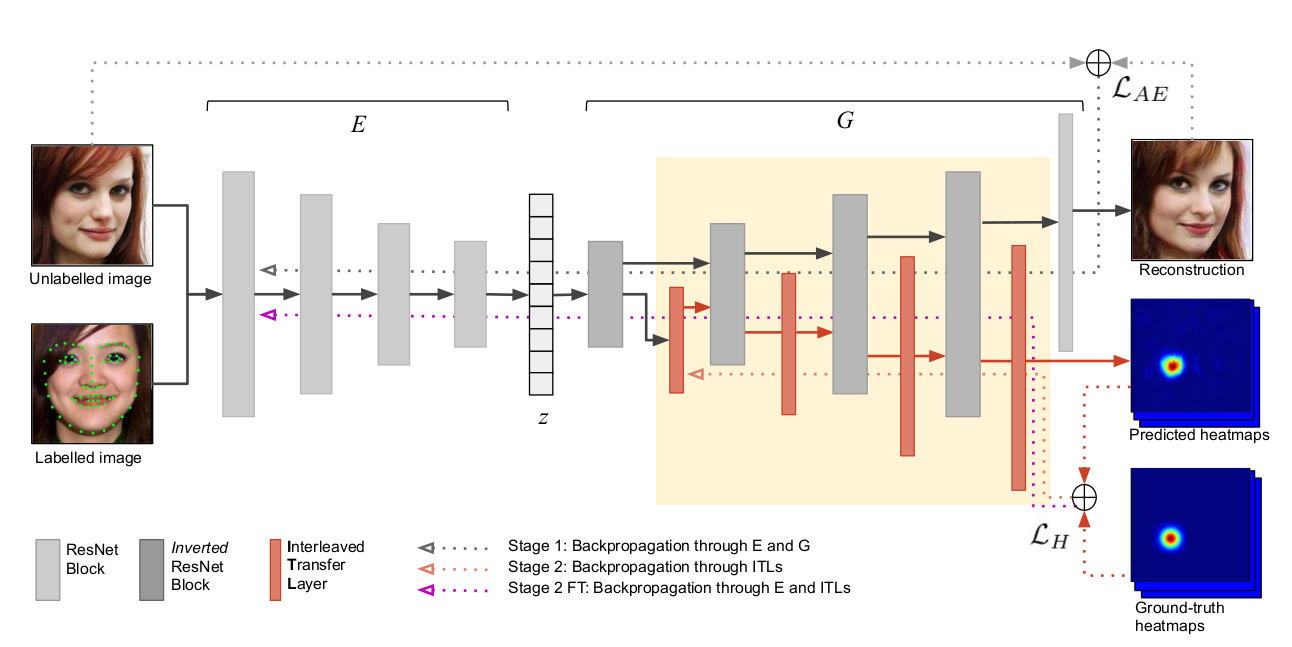
\includegraphics[width=0.98\textwidth]{img/3fabrec_arquitectura.png}
            \caption{Imagen resumen del framework 3FabRec. En ella podemos ver la estructura del \textit{Adversarial Autoencoder}, dividido en un Encoder (región bajo la \textit{E}) y un Generator (región bajo la \textit{G}). En rojo podemos ver las ITLs que se intercalan entre cada capa del Generador y dan como resultado un conjunto de mapas de calor. Imagen extraída de \cite{browatzki20203fabrec}.}
            \label{fig:3FabRec Resumen}
        \end{figure}

        \subsection{Arquitectura Adversarial Autoencoder}
            \noindent Para la construcción del \textit{Adversarial Autoencoder} utilizan:
            
            \begin{itemize}
                \item \textbf{Encoder}: emplean una ResNet-$18$  hasta codificar la entrada en un vector de $99$ dimensiones. Está pensado para imágenes de res $256 \times 256 \times 3$, aunque se adapta también a imágenes de dimensiones $512 \times 512 \times 3$.
                \item \textbf{Decoder}: emplean la misma red ResNet-$18$ pero invertida.
            \end{itemize}

            \noindent Para una mejor comprensión hemos realizado unos diagramas con la herramienta \textit{diagrams.net}. En la \autoref{fig:bloque_encoder} podemos ver la estructura básica de los bloques de la ResNet-$18$. Por otro lado en la \autoref{fig:Paso_encoder} podemos ver el paso de una imagen de entrada de tres canales y resolución $256 \times 256$ por el encoder.

            \begin{figure}[htbp]
                \centering
                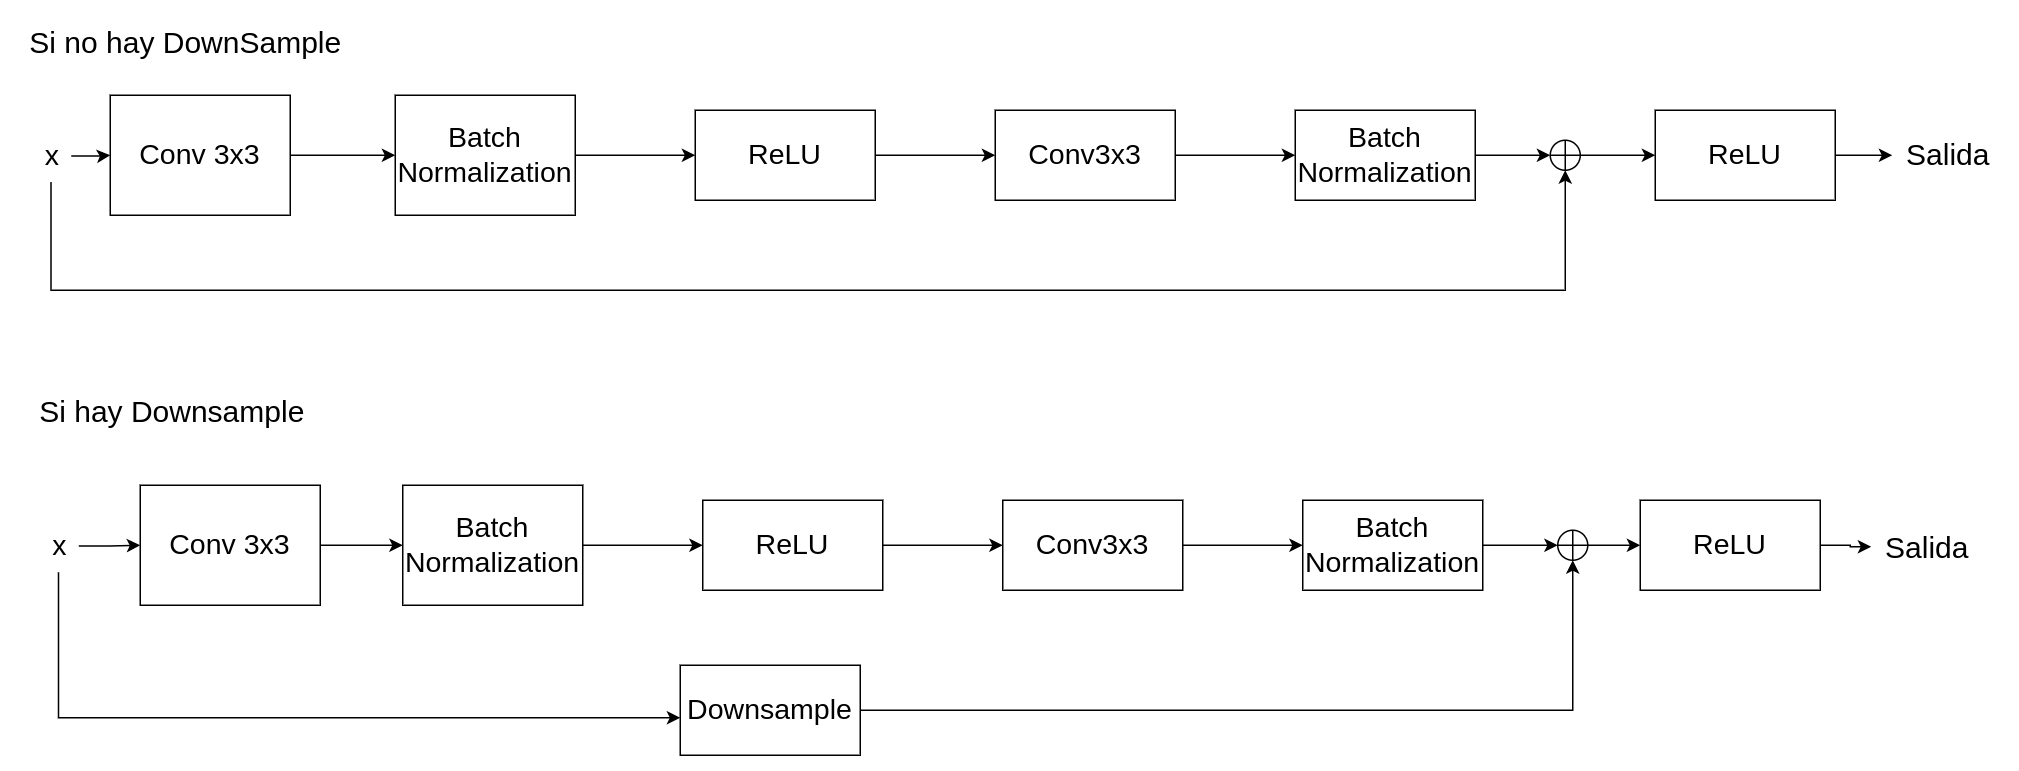
\includegraphics[width=0.95\textwidth]{img/bloque_basico_encoder.png}
                \caption{Bloques básicos que utilza la red ResNet-$18$ en sus capas. Se trata de una sucesión clásica de Convolución 3x3 + Batch Normalization + ReLU que se repite dos veces. En el primer caso los filtros de convolución no reducen las dimensiones del tensor añadiendo un padding de 1. En el segundo caso se reduce la dimensión del tensor a la mitad tras la primera convolución y se manteiene la dimensionalidad en la segunda. En el primer caso, la suma residual puede realizarse con el tensor x sin problema, en el segundo caso el tensor debe reducirse para que casen las dimensiones.}
                \label{fig:bloque_encoder}
            \end{figure}

            \begin{figure}[H]
                \centering
                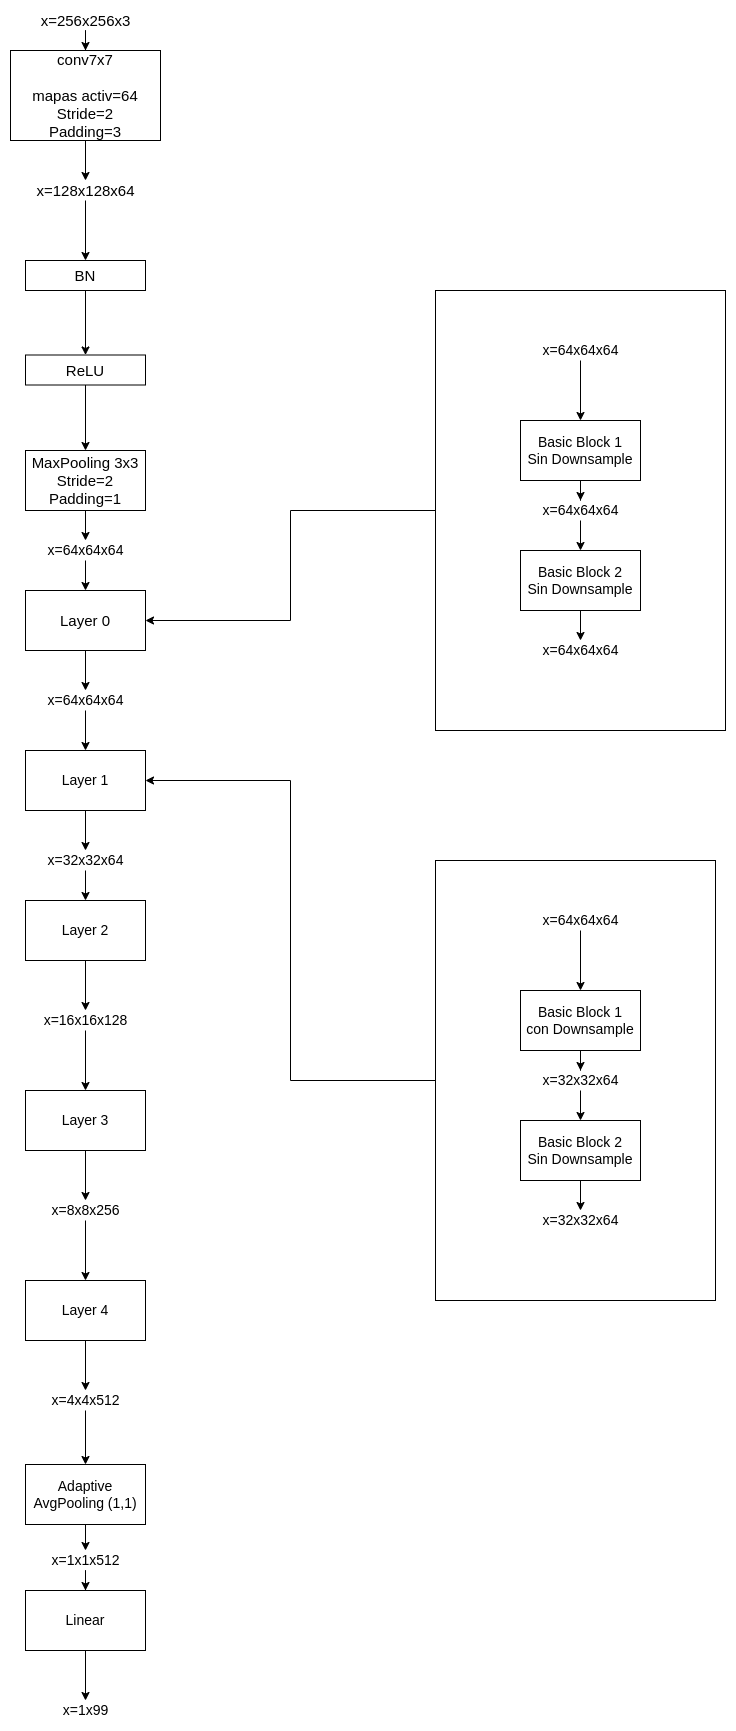
\includegraphics[width=0.7\textwidth]{img/3FabRec-Page-2.drawio.png}
                \caption{Ejemplo de paso de una imagen a través del Encoder. Cabe destacar que a partir de la Layer 1, todos los bloques tienen downsample.}
                \label{fig:Paso_encoder}
            \end{figure}

            \medskip

            \noindent En la \autoref{fig:Bloque_Decoder} podemos ver la estructura básica de un bloque en el Generador \textit{Inverse ResNet}, y un ejemplo del paso de un vector por el generador podemos verlo en la \autoref{fig:Paso_Generator}

            \begin{figure}[H]
                \centering
                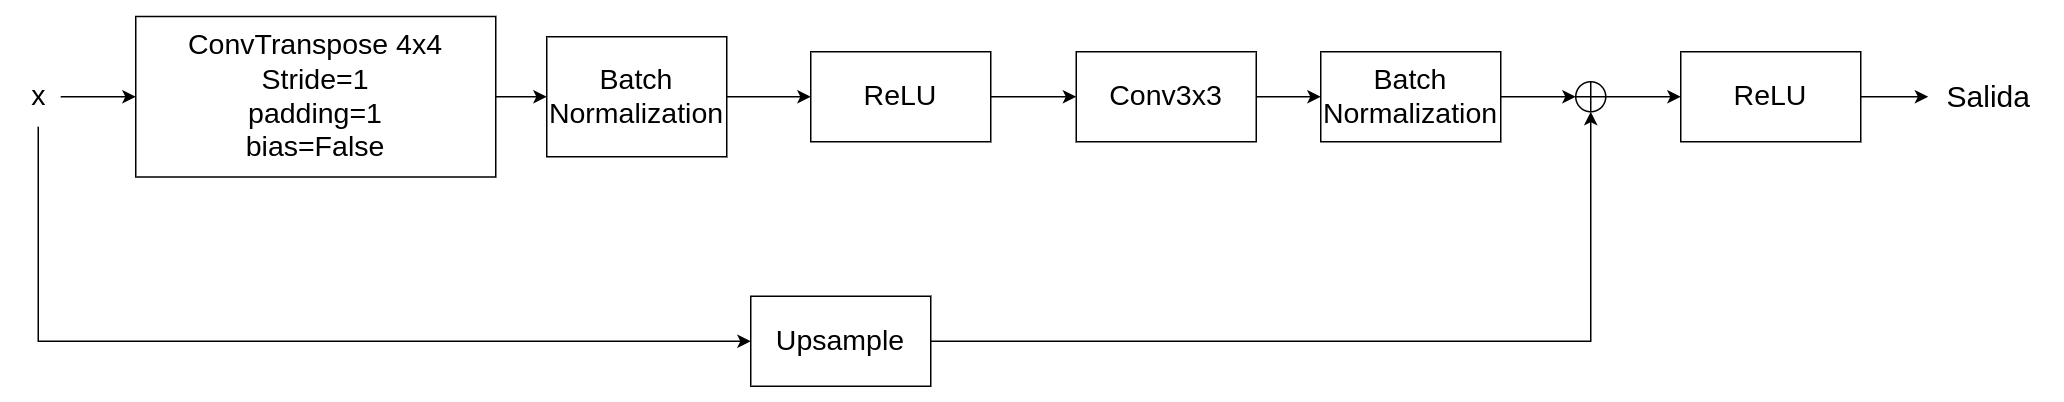
\includegraphics[width=0.96\textwidth]{img/bloque_invresnet.png}
                \caption{En primer lugar se aplica una convolución transpuesta que duplica las dimensiones del tensor de entrada y tras esto se sigue la misma estructura que en el bloque básico de la ResNet-$18$, la segunda convolución $3\times 3$ mantiene las dimensiones. Como consecuencia, para sumar el tensor de entrada con la salida del bloque se aumentan las dimensiones de este.}
                \label{fig:Bloque_Decoder}
            \end{figure}

            \begin{figure}[H]
                \centering
                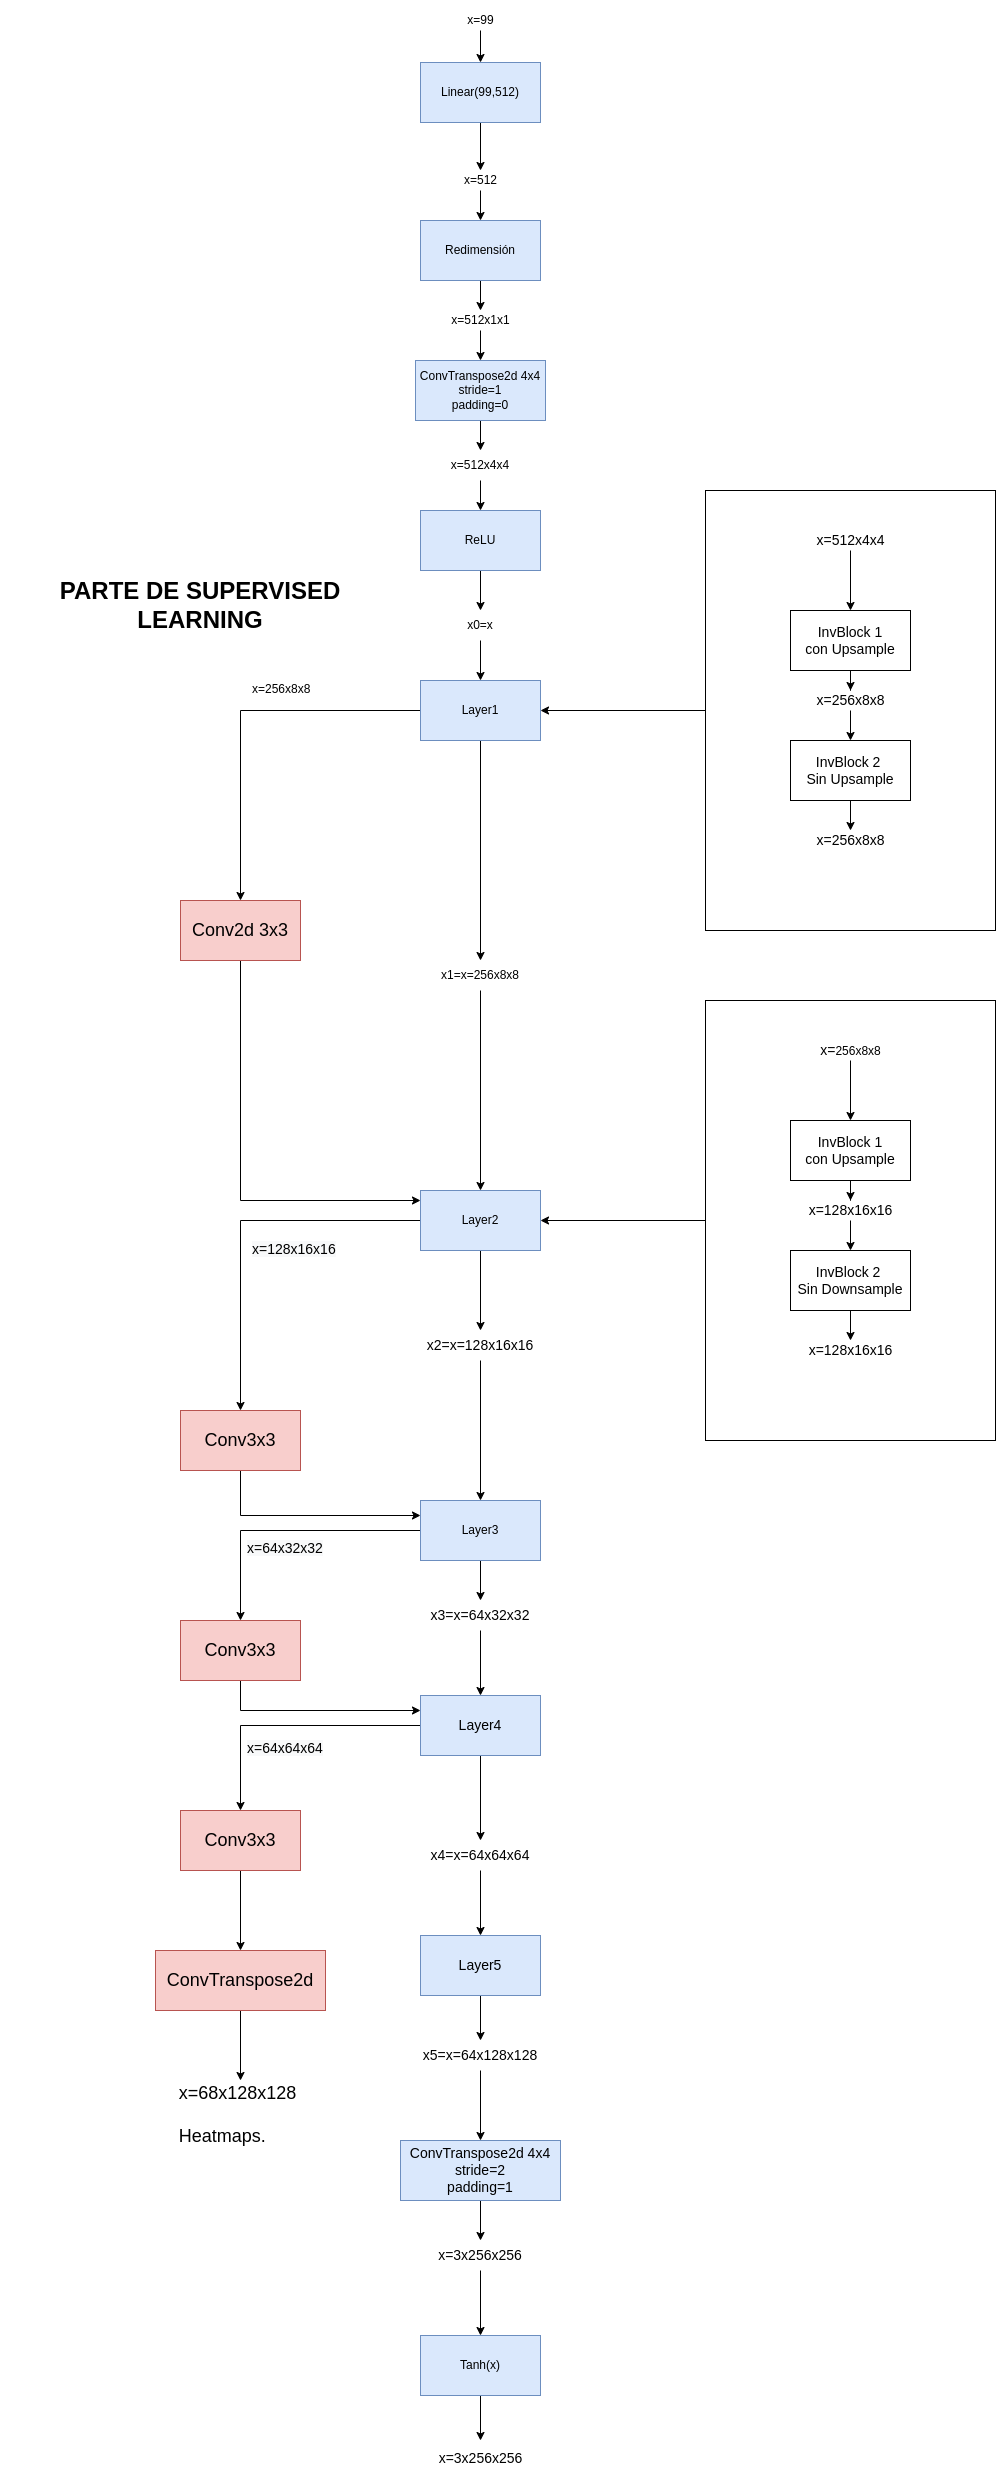
\includegraphics[width=0.95\textwidth]{img/paso_generator.png}
                \caption{Ejemplo del paso de un vector de $99$ dimensiones por el generador hasta reconstruirse la imagen de dimensiones $256 \times 256 \times 3$. La parte correspondiente al aprendizaje supervisado es la de los cuadrados azules, los cuadrados rojos corresponden a las \textit{ITLS} de la parte supervisada que se intercalan entre cada dos capas y dan como resultado los mapas de calor de los landmarks predichos.}
                \label{fig:Paso_Generator}
            \end{figure}

            \noindent Finalmente, necesitamos un Discriminador, que procure que los vectores del espacio vectorial latente sigan una determinada distribución. Dicha distribución será una normal multivariante estándar. Por otro lado, se añadirá un segundo discriminador propio de las redes \textbf{GAN} que nos dirá si la imagen reconstruida procede de la distribución que siguen los píxeles de la imagen de inicio. Este discriminador permite que la red genere imágenes más realistas. En la \autoref{fig:DGaussian} las redes neuronales que definen ambos discriminadores.

            \begin{figure}[H]
                \centering
                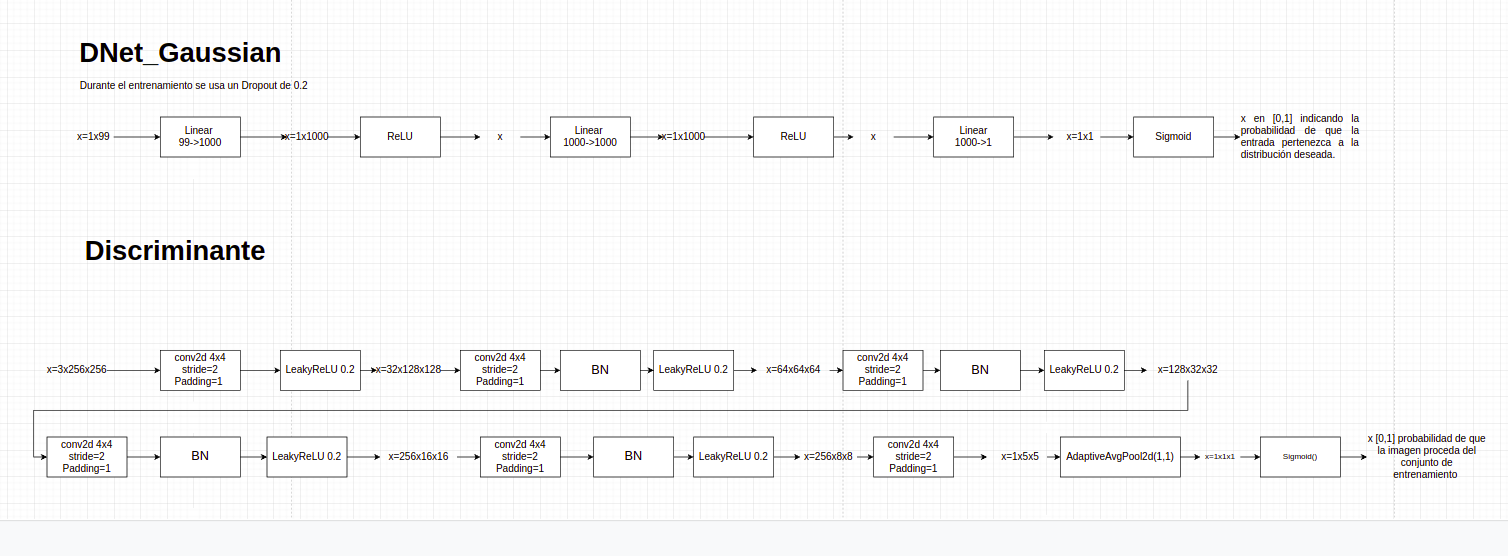
\includegraphics[width=0.95\textwidth]{img/DGaussian.png}
                \caption{En la imagen superior vemos el discriminante que se emplea para los vectores producidos por el Encoder y en la imagen inferior vemos el discriminante que se emplea para las imágenes generadas por el Generador. En ambos casos se da como salida un valor entre $0$ y $1$ que hace referencia a la probabilidad de pertenecer a la distribución deseada en el primer caso o a seguir la distribución de los píxeles de las imágenes en el segundo caso.}
                \label{fig:DGaussian}
            \end{figure}

            \subsubsection{Interleaved Transfer Layer (ITL)}
                \noindent Se denominan ITLs a las capas convolucionales encargadas de la predicción de landmarks. Se tratan de una solución novedosa porque premiten adaptar una AAE pensado originalmente para tareas de aprendizaje no supervisado a un problema de \textbf{regresión}, típico del aprendizaje supervisado.

                \medskip
                
                \noindent Se tratan de simples capas convolucionales que se intercalan entre las capas del Generador. La última de estas capas proporciona como salida un conjunto de mapas de calor, uno por cada landmark predicho. Estos mapas de calor luego se emplean para representar en la imagen reconstruida los landmarks. La arquitectura de esta etapa podemos verla en la \autoref{fig:Paso_Generator}.
            
        \subsection{Función de pérdida}

            \noindent La red utiliza dos funciones de pérdida, la primera que presentaremos se emplea en el entrenamiento del \textit{Adversarial Autoencoder}, en la parte no supervisada, y la segunda se utiliza tanto en la parte de aprendizaje supervisado como en la de \textit{fine-tuning} del Encoder. Debido al interés que tiene en el estudio del framework se van a presentar y explicar ambas funciones de pérdida. Cabe resaltar, que debido a que el problema que vamos a resolver es de \textbf{regresión}, en la fase de experimentación únicamente tendrá interés la segunda función de coste, asociada al entrenamiento de la parte supervisada.

            \medskip

            \noindent La función de pérdida empleada para el entrenamiento del \textit{Adversarial Autoencoder} en la parte de aprendizaje no supervisado es la siguiente: 
            
            \begin{align*}
                \min_{E,G} \max_{D_z,D_x} & \mathcal{L}_{AE}(E,G,D_z,D_x) = \\
                & \lambda_{rec} \mathcal{L}_{rec}(E,G) + \lambda_{cs}\mathcal{L}_{cs}(E,G) \\
                & + \lambda_{enc}\mathcal{L}_{enc}(E,D_z)+ \lambda_{adv} \mathcal{L}_{adv}(E,G,D_x)
            \end{align*}

            \noindent En la cual $\lambda_{enc}$ y $\lambda_{adv}$ toman el valor $1.0$ mientras que $\lambda_{rec}$ y $\lambda{cs}$ se establecen en $1.0$ y $60.0$ respectivamente. El valor de la función de coste se propagará por los pesos de $E$,$G$,$D_z$ y $D_x$ actualizándolos mediante \textit{back-propagation}. 

            \medskip

            \noindent Como podemos observar en la expresión anterior, se trata de una combinación lineal de cuatro funciones de coste distintas: 

            \begin{itemize}
                \item \textit{Error de reconstrucción}: Se trata de un error encargado de asegurarse de que la red reconstruya de forma apropiada las imágenes, para ello calcula la distancia $L_1$ entre la imagen original y la reconstruida pixel a pixel. Tiene la siguiente expresión, que coincide con la presentada en el apartado anterior de métricas.
                \begin{equation}
                    \mathcal{L}_{rec}(E,G)= \mathbb{E}_{x~p(x)}\left[\|x- G(E(x)) \|_1\right]
                \end{equation}
                \item \textit{Error estructural de la imagen}: Se trata de una variante del \textbf{SSIM} encargado de que la imagen real y la reconstruida tengan una estructura similar. La expresión de la función $cs$ que aparece en la fórmula se detalla más adelante.
                \begin{equation}
                    \mathcal{L}_{cs}(E,G)= \mathbb{E}_{x~p(x)}\left[cs(x, G(E(x)))\right]
                \end{equation}
                \item \textit{Error del Encoder}: es el error empleado comunmente en este tipo de redes y que se asegura que el vector latente que genera el encoder siga la distribución impuesta en el discriminador $D_z$. Su expresión es:
                \begin{equation}
                    \mathcal{L}_{enc}(E,D_z)=\mathbb{E}_{z^*~p(z)}[\log(D_z(z^*))] + \mathbb{E}_{x~p(x)}[\log(1-D_z(E(x)))]
                \end{equation}
                \item \textit{Error adversario de imagen}: normalmente las imágenes generadas por los Autoencoders suelen generar imágenes emborronadas. Es por ello que se introduce este error, que añade un discriminador típico de una red \textit{GAN} que pretende discernir entre si la imagen que recibe como salida de la red pertenece al conjunto de imágenes de entrenamiento o si es una imagen generada por la red, de esta forma se generan imágenes más realistas. Su expresión es la siguiente: 
                \begin{equation}
                    \mathcal{L}_{adv}(E,D_z)=\mathbb{E}_{x~p(x)}[\log(D_x(x))] + \mathbb{E}_{x~p(x)}[\log(1-D_x(G(E(x))))]
                \end{equation}
            \end{itemize}

            \medskip

            \noindent Por otro lado, la función de pérdida que se empleará en el \textbf{entrenmiento de las \textit{ITLs}} será la siguiente: 

            \begin{equation} \label{eq::L2}
                \mathcal{L}_H(ITL) = \mathbb{E}_{x ~ p(x)} \left[ \| H-ITL(a)\|_2 \right]
            \end{equation}

            \noindent Dónde $a$ serían los mapas de activación que genera la ResNet invertida para la imagen codificada $z=E(x)$ (siendo $x$ la imagen de entrada a la red). En este caso se computa la distancia \textbf{$L_2$} entre los \textit{Heat-maps} de los lanmarks originales de la imagen $x$ de entrada, y los predichos por las \textit{ITLs}. Propagando el error por los pesos de las \textit{ITLS} solamente, forzando a adaptarse a los pesos ya aprendidos del generador.

            \medskip

            \noindent A modo de aclaración, las imágenes etiquetadas con landmarks a la red suelen proporcionarse con el siguiente formato: 

            \begin{itemize}
                \item Un archivo con la imagen sin etiquetar. 
                \item Un archivo de texto plano con las coordenadas de cada landmark en la imagen.
            \end{itemize}

            \noindent Dados estos archivos, el framework, calcula para cada landmark proporcionado un mapa de calor en una imagen de tamaño $128 \times 128$ en el caso de que las imágenes de entrada sean de $256 \times 256$. Y es a ese conjunto de imágenes (una por cada landmark) a las que denominamos $H$ en la función anterior.

            \medskip

            \noindent Finalmente, en la etapa de \textit{fine-tuning} se computa la misma función de pérdida de antes, con la salvedad de que el error se propaga tanto por las \textit{ITLs} como por los pesos del \textit{Encoder}. Esto permite que el \textit{Encoder} se codifiquen con mayor precisión las imágenes y que se eliminen factores irrelevantes para la predicción de landmarks como son el género, el color de piel o la iluminación. Por otro lado se evita el overfitting ya que durante esta última etapa los pesos del \textit{Decoder} no se actualizan.

        \subsection{Proceso de entrenamiento de la red}

            \subsubsection{Entrenamiento no-supervisado}
                \noindent El framework que empleamos ha sido entrenado durante $50$ épocas con imágenes de tamaño $256x256$ y con un tamaño de batch de $50$. En todas las etapas del entrenamiento se ha empleado un optimizador tipo Adam, el cual durante el entrenamiento del \textit{Adversarial Autoencoder} usó $\beta_1=0.0$ y $\beta_2=0.999$ con un \textit{learning rate} de $2\times 10^{-5}$.

                \medskip

                \noindent Por otra parte, se aplicaron técnicas de \textit{data-augmentation} a las imágenes de entrada como giros horizontales, traslaciones, \textit{resizing} o rotaciones.

            \subsubsection{Entrenamiento supervisado}
                \noindent Para el entrenamiento de la parte supervisada, las imágenes de entrada se recortan de acuerdo a un \textit{bounding-box} creado por el framework a partir de unas coordenadas de entrada o bien de acuerdo a los landmarks que se proporcionan. Tras el recorte, se reescala la imagen hasta tener un tamaño de $256\times256$. 
                
                \medskip

                \noindent Por otro lado se crean los \textit{Heat-maps} para cada landmark. Para esto se crea una imagen de tamaño $128 \times 128$ por cada landmark marcando el punto con ayuda de una distribución normalde dos dimensiones centrada en las coordenadas del landmark y usando una desviación típica de $\sigma=7$.

                \medskip

                \noindent Tras esto se entrenan las cuatro \textit{ITLs}. A los datos de entrada se les aplican técnicas de \textit{data-augmentation} como rotaciones, traslaciones, reescalados y oclusiones. Para esta etapa se usa también un optimizador Adam con un \textit{learning rate} de $0.001$ y los mismos valores para $\beta_1$ y $\beta_2$.

                \medskip

                \noindent Finalmente, durante la etapa de \textit{fine-tuning} se establece un \textit{learning-rate} de $0.0001$ en las \textit{ITLs} mientras que el del \textit{Encoder} se mantiene en su valor por defecto de $2 \times 10^{-5}$ y cambiando el valor de $\beta_1 = 0.9$.

        \subsection{Bases de datos usadas por el framework}
            
            \noindent Para el entrenamiento no supervisado del \textit{AAE}, se emplearon los siguientes datasets unidos: 

            \begin{itemize}
                \item \textbf{VGGFace2} : Contiene un total de $3.3$ millones de imágenes de rostros en distintas poses, edad, iluminación, etnia, etc \ldots  Del dataset eliminaron las imágenes de rostros que tuviera una altura menor a $100$ píxeles, quedando un total de $1.8$ millones de caras.
                \item \textbf{AffectNet} : Se trata de un dataset de $228$ mil imágenes en una gran variedad de poses, iluminación, etc..
            \end{itemize}

            \noindent En total usaron unas $2.1$ millones de imágenes.

            \noindent Para el entrenamiento supervisado se emplearon los siguientes datasets: 

            \begin{itemize}
                \item \textbf{300-W} : une diversos datasets de rostros etiquetados con \textbf{$68$}landmarks de manera semi-automática como son \textbf{LFPW},\textbf{AFW}, \textbf{HELEN} y \textbf{XM2VTS}. Además de añadir datos propios. En total emplearon $3,148$ (aproximadamente el $80 \%$ )imágenes para el entrenamiento y $689$ para test, las cuales se dividieron en dos grupos, uno de $554$ imágenes considerado el grupo test estándar, y otro de $135$ imágenes difíciles.
                \item \textbf{AFLW} : contiene un total de $24,386$ imágenes \textit{in-the-wild} con un amplio rango de poses distintas. Se emplearon $20,000$ (aproximadamente el $80 \%$) imágenes para test y $4,386$ para entrenamiento. Las imágenes vienen etiquetadas con $21$ landmarks, pero en el framework se entrena la red para predecir \textbf{$19$}.
                \item \textbf{WFLW}: Es la más reciente de las empleadas y tiene un total de $10,000$ imágenes. Se usan $7,500$ para entrenamiento y $2,500$ para test. Las imágenes tienen un total de \textbf{$98$} landmarks anotados.
            \end{itemize}

            \medskip

            \noindent Como podemos observar, los conjuntos de datos disponibles para el entrenamiento de redes especializadas en la identificación de landmarks faciales son variados y con muchos ejemplos de entrenamiento. En nuestro caso concreto, no contamos con tantos ejemplos y apenas hay bases de datos forenses con landmarks cefalométricos, lo cual es una dificultad añadida al problema, pues solo podremos entrenar con los datos que se nos proporcionan y como veremos son muy pocos.

\section{Métricas}

\noindent En esta sección, se van a presentar las principales métricas de error que se emplearán para estudiar la bondad de los resultados que se obtengan en futuros capítulos.

    \subsection{Métricas usadas en el entrenamiento}
        \noindent Las métricas que se muestran durante el entrenamiento utilizadas por el modelo son:

        \subsubsection{MSE}
            \noindent Se trata del error cuadrático medio, una función empleada típicamente en problemas de regresión y que tiene la siguiente expresión: 

            \begin{equation}
                MSE = \frac{1}{N} \sum_{i=1}^{N} (y_i - \widehat{y}_i)^2
            \end{equation}

            \noindent En nuestro caso concreto, este error se calcula entre los mapas de calor de los landmarks reales y predichos a nivel de pixel, es decir $y_i$ en la fórmula anterior corresponde a cada pixel del heatmap del landmark real y por tanto $\widehat{y}_i$ es el valor del pixel correspondiente en el heatmap predicho. Dichas diferencias se suman en todos los heatmaps y se divide por $N$ que en este caso es el número total de píxeles juntando todos los Heat-maps.

            \medskip

            \noindent Este error se empleará para realizar \textit{backpropagation} a través de las ITLs de la red y será el responsable del aprendizaje de la red.

    \subsection{Métricas empleadas en validación y testing}

        \subsubsection{Error de reconstrucción}
            \noindent El valor del error de reconstrucción en las imágenes de validación nos llevará en la sección de experimentación a realizar hipótesis sobre la relación entre este error y el NME.

            \medskip

            \noindent Se trata de la función de coste \textbf{L1} que se aplica a la imagen original y la reconstruida  y nos porporciona una medida del error de reconstrucción a nivel de pixel. Su expresión es la siguiente:

            \begin{equation}
                Reconstruction \; Loss = \frac{\sum_{i=1}^n |p_i -q_i|}{N}
            \end{equation}

            \noindent Donde $p_i$ representa cada pixel de la imagen reconstruida por la red, $q_i$ el equivalente en la imagen real y $N$ el total de píxeles presentes en la imagen.

        \subsubsection{Normalized Mean Error}
            \noindent Este será el error utilizado para medir la bondad de los resultados. Tiene la siguiente expresión para cada landmark de los $30$: 

            \begin{equation}
                NME=\frac{\sqrt{\sum_{i=1}^{n}(p_{i,1} -q_{i,1})^2+ (p_{i,2} -q_{i,2})^2}}{N}
            \end{equation}


            \noindent Así, si en total se han identificado en las imágenes de validación un total de $n$ landmarks de cierto tipo en las imágenes de test o validación, se calcula la distancia $L_2$ entre el landmark de la imagen $i$ predicho y el real. Y tras esto se suman todos los valores obtenidos. Como podemos ver, idealmente $n$ debería ser el total de imágenes que hay en validación o test, pero no todos los landmarks aparecen en todas las imágenes, por lo tanto $n\leq M$ siendo $M$ el total de imágenes en validación.

            \noindent En dicha expresión $N$ es el término por el que se normaliza, y varía según el problema. En nuestro caso normalizaremos la media del numerador por el ancho de la imagen que es de $256$ píxeles, ya que la distancia máxima permitida entre dos landmarks sería esta, y así todos los valores quedarían entre $0$ y $1$ siendo $0$ una estimación perfecta del landmark, y $1$ un error total en el marcado. Es importante la normalización debido a la heterogeneidad de los tamaños de los datos de entrada. Así, el NME extraído en cada dato es comparable con los del resto.

            \subsubsection{SSIM}
            \noindent Se trata del \textit{structural similarity index} (SSIM) y da una medida de \textit{similaridad} entre dos imágenes \cite{wang2004image}, su expresión es la siguiente: 

            \begin{equation}
                SSIM(x,y)=[l(x,y)]^\alpha[c(x,y)]^{\beta}[s(x,y)]^{\gamma}
            \end{equation}

            \medskip

            \noindent Dónde $x,y$ son las dos imágenes que van a ser comparadas.

            \medskip

            \noindent La componente $c(x,y)$ hace referencia a la función de comparación del contraste de las dos imágenes y viene dada por la siguiente expresión: 

            \begin{equation}
                c(x,y)=\frac{2\sigma_x \sigma_y + C}{\sigma_x^2+ \sigma_y^2+C}
            \end{equation}

            \noindent Dónde $\sigma_x, \sigma_y$ hacen referencia a la desviación estándar de cada imagen.

            \medskip

            \noindent La componente $s(x,y)$ es la función de comparación estructural entre las dos imágenes y viene dada por la siguiente expresión:

            \begin{equation}
                s(x,y)=\frac{\sigma_{xy}+C/2}{\sigma_x \sigma_y +C/2}
            \end{equation}

            \noindent Dónde $\sigma_{xy}$ denota la covarianza.

            \medskip

            \noindent La componente $l(x,y)$ hace referencia a la \textit{luminosidad}, pero en el caso de 3FabRec se prescinde de esta componente, además los exponentes $\alpha, \beta , \gamma$ se igualan a $1$.

            \medskip

            \noindent Por otra parte siguen las indicaciones del paper original de SSIM que recomiendan usar estas comparaciones en regiones de la imagen y promediarlas en vez de aplicarlas sobre todo el conjunto de píxeles de la imagen, es por ello que la expresión final queda:

            \begin{equation}
                cs(x,y)=\frac{1}{|w|} \sum{c(x_w,y_w)s(x_w,y_w)}_w
            \end{equation}

            \noindent Dónde $w$ representa la ventana sobre la que se aplica la función y $|w|$ el total de ventanas. En nuestro caso se emplean ventanas de tamaño $31\times 31$.

\section{Preprocesamiento de los datos}
        
        \subsection{Identificación de caras en las imágenes}
            \noindent Antes de poder entrenar el modelo, es necesario adecuar el dataset para que pueda usarse modelo. El framework está pensado para recibir como entrada una imagen, a la cual, se le hace un recorte a la región que ocupa el rostro con ayuda de un \textit{bounding box} predefinido y determinado por las coordenadas en la imagen de las cuatro esquinas o bien siguiendo los landmarks descritos por el fichero auxiliar asociado a cada imagen. En nuestro caso, debido a que la mayoría de landmarks son internos y no se suelen situar en los bordes de la cara, hemos pensado que la mejor manera de entrenar la red es que se realice el recorte de la imagen de entrada de acuerdo a un \textit{bounding box}. Para ello fue necesario emplear una red especializada en la detección de caras en imágenes y que nos proporcionaba como salida una lista con los \textit{bounding boxes} de todas las caras detectadas. La red se denomina \textbf{Facenet}, y se puede importar de la librería \textit{facenet} de \textit{pytorch} como \textit{mtcnn}.

            \medskip

            \noindent Así pues, se realizó un primer estudio para determinar los mejores parámetros para \textit{facenet}. Existen muchos parámetros editables, pero la mayoría se dejaron con sus valores por defecto, únicamente se consideró modificar: 

            \begin{enumerate}
                \item \textbf{image\_size}: Determina el tamaño de la imagen de salida.
                \item \textbf{select\_largest}: Si su valor es \textit{true}, se devuelve la cara más grande detectada, y si su valor es \textit{false}, se devuelve la de mayor confianza detectada.
            \end{enumerate}


            \noindent En nuestro caso, primero se probó con un \textit{image\_size} de $256 \times 256$, pero esto tenía problemas pues en ocasiones no podían construirse \textit{bounding boxes} de este tamaño y producían error, por lo que se redujo a $128 \times 128$. Por otro lado, observando las imágenes del dataset de entrenamiento, nos dimos cuenta que en algunas imágenes aparecían varios sujetos, y en ocasiones la cara más \entrecomillado{grande} mo pertenecía al sujeto principal. Es por ello que se decidió establecer el parámetro \textit{select\_largest} a \textit{False}, y así obtener como salida una lista de \textit{bounding boxes} ordenados de mayor a menor según el nivel de confianza. No obstante, en algunos casos se tuvo que elegir con cuidado cuál de los bounding boxes proporcionados se correspondía con el sujeto principal.

            \medskip

            \noindent Una vez establecidos los parámetros, se detectaron problemas en la identificación de caras en algunas imágenes. Debido a que todas las imágenes erróneas estaban en escalas de grises nos dimos cuenta de que la red sólo acepta como entrada imágenes en tres canales, por lo que cada imagen en escala de grises de un solo canal tuvimos que replicar tres veces su canal. 
        
            \medskip
        
            \noindent Tras esto, volvimos a ver que en algunas imágenes no se detectaban \textit{bounding boxes}. Esto nos llevó a realizar un breve estudio sobre si era buena idea continuar usando esta red o buscar otra. En este estudio clasificamos las imágenes en tres grupos y aplicamos la red a cada uno de ellos por separado: 

            \begin{enumerate}
                \item Imágenes de sujetos en posición \textbf{ frontal}: en total hay $87$ imágenes frontales de las cuales se extraen correctamente el \textbf{$100\%$} de los \textit{bounding boxes}.
                \item Imágenes de sujetos en posición de \textbf{$3/4$}: En este caso hay $57$ imágenes de las cuales el \textbf{$100\%$} de los \textit{bounding boxes} extraidos por la red son correctos.
                \item Imágenes de sujetos en posición de \textbf{perfil}: En este caso hay un total de $23$ imágenes y se clasifican correctamente $20$, lo que supone una precisión del \textbf{$87\%$}. Además, las imágenes que fallaban estaban en escala de grises y con malas condiciones de calidad e iluminación.
            \end{enumerate}

            \medskip

            \noindent Por lo tanto, debido al bajo número de ejemplos en los que la red falla, se decidió mantener la red \textbf{Facenet} para determinar los \textit{bounding boxes} y además se excluyeron los tres ejemplos dónde fallaba del dataset, y se descartó otro ejemplo por tener los landmarks marcados de forma incorrecta. Esto hizo que en total se usaran $163$ de las $167$ imágenes originales.

            \medskip 

            \begin{figure}[H]
                \centering
                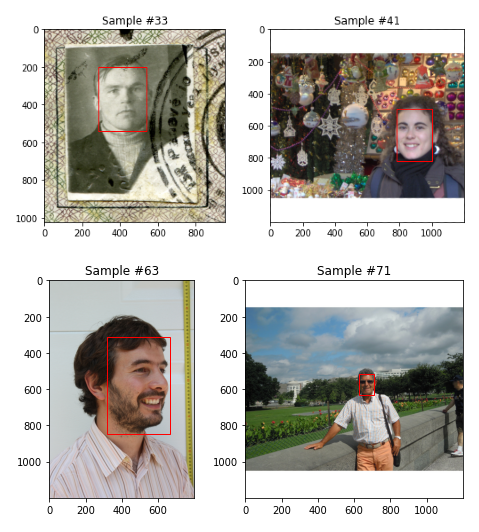
\includegraphics[width=0.7\textwidth]{img/imagenes_ejemplo_bb.png}
                \caption{Imágenes de ejemplo del dataset con los \textit{bounding boxes} marcados por \textit{Facenet}. Como podemos observar, aunque son correctos, los \textit{bounding boxes} marcados recortan excesivamente los límites del rostro, pudiendo incluso eliminar partes en las que hay landmarks marcados. Las imágenes han sido generadas con \textit{matplotlib}.}
                \label{fig:Ejemplo_bb}
            \end{figure}

            \noindent Durante el estudio anterior, se observaron otros hechos dignos de mención. En primer lugar se identificaron dos imágenes repetidas, pero se decidió mantenerlas pues los landmarks presentes en una y otra eran diferentes, lo que podía ayudar al entrenamiento. Por otro lado, durante el entrenamiento se vió cómo había una imagen de un determinado sujeto en la que aprecían simultáneamente dos fotos, una  de frente y otra de perfil. Sin embargo, al estar los landmarks anotados únicamente en la imagen de frente se tomó el \textit{bounding box} de la imagen frontal desechando el otro para el perfil. En otras dos imágenes se pueden ver un conjunto de varias personas, y la red mostraba erróneamente los \textit{bounding boxes} de personas que no eran el sujeto de estudio, por lo que estudiar cuál de todos los \textit{bounding boxes} devueltos pertenecía al sujeto correcto.

            \medskip

            \noindent Además de todo lo anterior, se descubrió que una imagen tenía los landmarks marcados de forma incorrecta. Estp nos llevó a descartarlo para los experimentos, y así empleamos en total $163$ imágenes para el estudio.

        \subsection{Creación del fichero annotations en el dataset}

            \noindent Una vez se identificaban correctamente todos los \textit{bounding boxes}, siguiendo como inspiración el dataset \textit{AFLW}, se generó un fichero denominado \textit{annotations.csv} dentro de la carpeta del proyecto en el que encuentra el dataset. En este fichero se almacenó \textbf{para cada imagen} una serie de datos: 

            \begin{itemize}
                \item El nombre del fichero.
                \item El índice de la imagen dentro del dataset. 
                \item Una lista con las coordenadas $2D$ de cada landmark en la imagen (incluidos los no presentes como situados en la posición $[-1,-1]$). 
                \item Una lista denominada máscara, que representa la visibilidad de cada landmark en la imagen. Los landmarks visibles en la imagen tienen asociado el valor $1$, mientras que los no visibles tienen asociado el valor $0$. Esta máscara será de gra utilidad a la hora de extraer las métricas, pues hay que realizar las medias de acuerdo al número de landmarks visibles de cada tipo, no se puede usar siempre el valor $30$.
                \item Finalmente, se almacena la posición en coordenadas de la esquina inferior izquierda del \textit{bounding box} junto con el ancho y el alto, para que el framework recorte la imagen quedándose con el rostro únicamente. 
            \end{itemize}

        \subsection{Reajuste de los bounding boxes}
            \noindent Finalmente, como parte del proceso de determinar los \textit{bounding boxes}, se vió que en todos los casos, dichos rectángulos cortaban parte de las caras de los sujetos (partes en las que había landmarks marcados). Es por ello, que se tuvo que realizar una transformación del \textit{bounding box} sugerido para que manteniendo el centro del mismo abarcase una mayor superficie y que contuviera el rostro completo del sujeto. 

            \medskip

            \noindent La transfomación consiste en desplazar la esquina superior izquierda del rectángulo una cantidad \textit{m} en el eje de ordenadas y abscisas y establecer el resto de esquinas de acuerdo a este parámetro como se muestra en la \autoref{fig:Transformacion_BB}.


            \begin{figure}[!h]
                \centering
                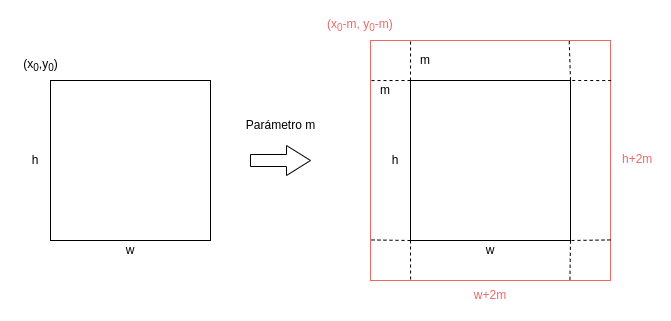
\includegraphics[width=0.8\textwidth]{img/Transformacion_rectangulo.png}
                \caption{Proceso seguido para la transformación.}
                \label{fig:Transformacion_BB}
            \end{figure}

            \begin{figure}[!h]
                \centering
                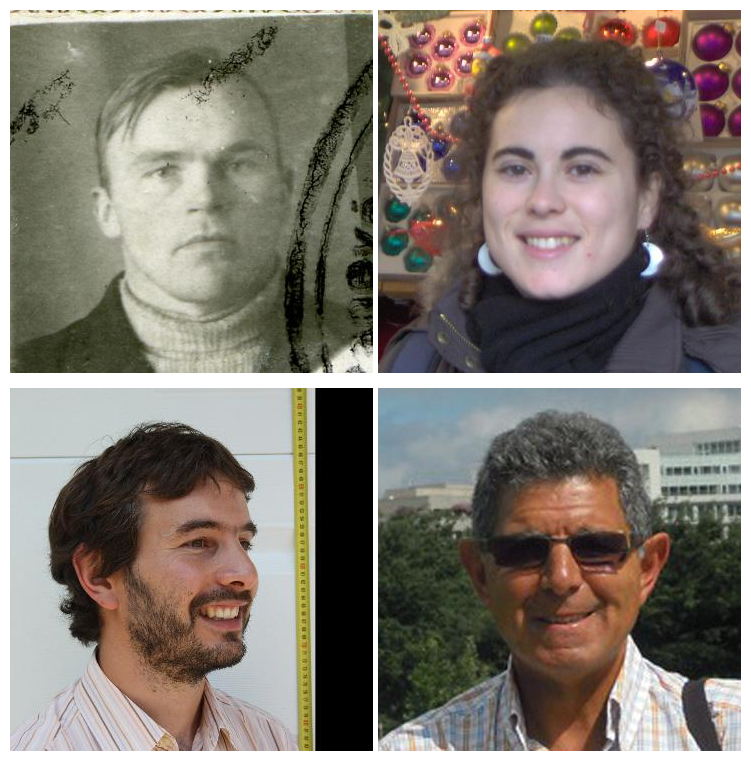
\includegraphics[width=0.7\textwidth]{img/imagenes_ejemplo_cropping.png}
                \caption{Recorte de las caras tras el reajuste del \textit{bounding box}.}
                \label{fig:Reajuste_bb}
            \end{figure}

            \medskip

            \noindent No obstante, el framework 3FabRec dispone de un método de recorte y redimensión automático de las caras empleando \textit{bounding boxes}. En un primer momento, forzamos al framework a respetar los \textit{bounding boxes} construidos durante el preprocesamiento, pero los errores de reconstrucción de estas imágenes eran muy elevados. No resultaba práctico para entrenar la red, pues el framework marca los puntos sobre localizaciones que no guardaban parecido con el lugar real del punto en la imagen original. Podemos ver algunos ejemplos de reconstrucción en la \autoref{fig:bb_custom}.


            \begin{figure}[!h]
                \centering
                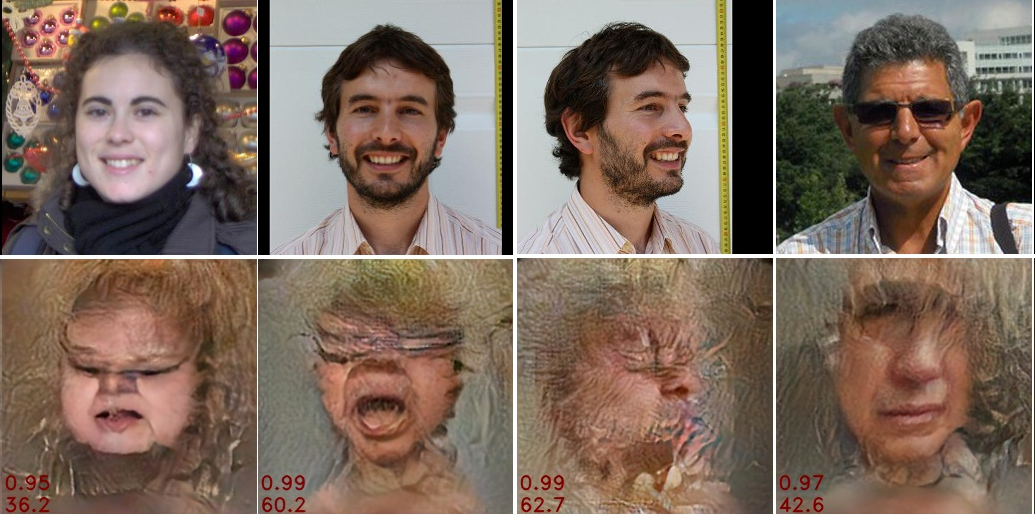
\includegraphics[width=0.7\textwidth]{img/bounding_box_custom.png}
                \caption{Error estructural y de reconstrucción de las imágenes con el bounding box reajustado. El error de reconstrucción se encuentra en la esquina inferior izquierda, y el estructural encima del anterior. Como podemos observar, en todos los casos son muy elevados y la imagen reconstruida apenas guarda relación con la original.}
                \label{fig:bb_custom}
            \end{figure}

            \medskip

            \noindent Se probó entonces a aplicar al \textit{bounding box} definido, el reajuste que realiza 3FabRec. Este nuevo reajuste dejaba en la mayoría de casos mal marcado el \textit{vertex}, pues suele recortar la parte superior de la cabeza. No obstante los errores de reconstrucción eran mucho menores con esta alternativa y los landmarks predichos se localizaban en las imágenes reconstruidas sobre puntos que guardaban una estrecha relación con la localización real en la imagen original (véase la \autoref{fig:bb_3fabrec}). Se decidió entonces estudiar por qué ocurría esto.

            \begin{figure}[!h]
                \centering
                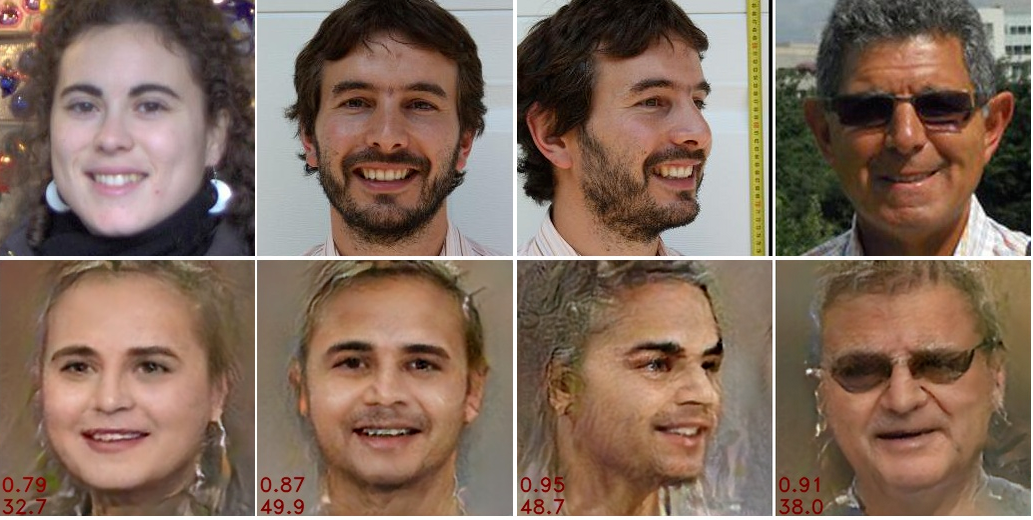
\includegraphics[width=0.7\textwidth]{img/bounding_box_3fabrec.png}
                \caption{Error estructural y de reconstrucción de las imágenes con el reajuste del bounding box de 3FabRec. Como podemos ver, sigue habiendo grandes errores de reconstrucción y estructurales, pero se consigue un mejor resultado de la estructura facial. No obstante, el vertex no se aprecia correctamente en las imágenes.}
                \label{fig:bb_3fabrec}
            \end{figure}

            \noindent El reajuste que realiza 3FabRec es el siguiente:
            \begin{enumerate}
                \item En primer lugar, se determina el tamaño de la región de interés (ROI, del inglés region of interest) en píxeles. Para ello, el framework por defecto calcula la diagonal del tamaño de las imágenes de entrada (en nuestro caso son $256 \times 256$), y lo redondea al entero superior más próximo (el resultado es de $363$ píxeles, en nuestro caso). De este valor se obtienen dos parámetros, el \textit{crop\_size} y el \textit{margin}, de manera que \textit{crop\_size + margin = roi} (en nuestro caso \textit{crop\_size}=$256$ y \textit{margin}=$107$).
                \item En segundo lugar, se reajusta el bounding box convirtiéndolo siempre en cuadrado de lado $\max(ancho,alto)$. Se calcula el factor de escalado $escala = \frac{crop\_size + margin}{crop\_size}$, para ampliar el bounding box original uniformemente, de acuerdo al margin. 
                \item  Finalmente se reescala el resultado a una imagen de tamaño $256\times 256$.
            \end{enumerate}

            \medskip

            \noindent Por otro lado, el entrenamiento no supervisado del \textit{AAE} hizo que la red aprendiera la distribución de un determinado dataset de imágenes. Estudiando minuciosamente los ficheros encargados de preparar los datos de entrenamiento (affectnet.py y vgg2face.py), se vio que en ambos, el tamaño de las imágenes es de $256 \times 256$, pero no se especifica un valor determinado para el ROI, por lo que este se calcula por el framework de la misma manera que hace con nuestras imágenes, realizando un ajuste de los bounding boxes idéntico al nuestro. Además, para el ajuste fino del encoder utilizando las imágenes de \textit{AFLW}, de nuevo se aplicaron estas transformaciones.
            
            \medskip
            
            \noindent Esto, puede explicar por qué en el primer caso no se reconstruyen bien las imágenes, ya que se fuerza a que no se apliquen estas transformaciones a las imágenes de entrada. De esta manera, la distribución de las imágenes de entrada cambia radicalmente con respecto a la distribución con la que fue entrenada la red y su posterior \textit{fine-tuning} con \textit{AFLW}. Sin embargo, si permitimos que 3FabRec realice las transformaciones descritas anteriormente, conseguimos que la distribución de los datos de entrada (pese a seguir siendo diferente) sea lo mas \entrecomillado{parecida} posible a la distribución sobre la que fue entrenada la red, mejorando la reconstrucción de las imágenes. 
            
            \medskip
            
            
            \noindent Por lo expuesto anteriormente, se decide continuar con el reajuste que realiza el framework para lograr una mejor reconstrucción, aunque se pierda el marcado correcto del \textit{vertex}.

    \subsection{Separación en conjuntos de entrenamiento y validación}
        \noindent Separamos la base de datos proporcionada en conjuntos de entrenamiento, validación y test. Por el limitado número de ejemplos que tenemos, será necesario emplear \textbf{validación cruzada} para la elección entre los modelos que se prueben. Así pues, de las \textbf{163 imágenes} que usaremos en total, establecemos una semilla para que los procesos aleatorios sean replicables en cualquier máquina y con ayuda de la función \textit{random-shuffle} de python separamos los datos en: 

        \begin{itemize}
            \item \textbf{Conjunto de test}: 32 imágenes ($20\%$ del total de imágenes).
            \item \textbf{Conjunto de entrenamiento:} 131 imágenes ($80\%$ del total de imágenes).
        \end{itemize}

        \noindent Por otro lado, el conjunto de entrenamiento se subdivide a su vez en cinco subconjuntos, con la idea de realizar \textbf{5-fold cross-validation}. Cada subconjunto estará compuesto por \textbf{26 imágenes} exceptuando el último que tendrá \textbf{27}.
        
        \medskip

        \noindent Para esta técnica se realizan cinco ejecuciones independientes en la cual se toman cuatro de los cinco subconjuntos de entrenamiento para entrenar el modelo y se deja el último subconjunto para validar el modelo. Así, en cada iteración se cambia el conjunto que se empleará para validación, con la finalidad de mejorar la calidad de las decisiones que se tomen sobre el rendimiento, pues la decisión estará mejor informada.

        \medskip

        \noindent Con cada propuesta de modelo, se medirá su rendimiento usando \textbf{5-fold cross-validation}, obteniendo 5 salidas de validación para cada modelo. Cada salida se compone de una tabla en la que aparece el NME medio por landmark (teniendo en cuenta sólamente los marcados en validación), y una tabla en la que para cada imagen de validación se obtiene su NME medio (haciendo la media del NME cometido por cada landmark), y el error de reconstrucción. Para la elección del modelo final se tendrá en cuenta: 

        \begin{itemize}
            \item Una tabla en la que se promedian las cinco tablas obtenidas con el NME medio por landmark.
            \item Una tabla en la para cada imagen del conjunto de entrenamiento, se tiene el NME cometido y el error de reconstrucción. Esta tabla se obtiene concatenando todas las predicciones de cada partición de cross-validation.
        \end{itemize}


\section{Experimentación}
    \subsection{Hipótesis iniciales}
        \noindent Debido a que partimos de \textbf{3FabRec}, un framework diseñado y probado de forma exahustiva por Björn Browatzki y Christian Wallraven, en los experimentos se va a respetar la arquitectura de la red en su totalidad, sin añadir ni eliminar capas. Del mismo modo, debido a que la elección del optimizador \textbf{Adam} empleado por los autores ha sido fruto de un proceso de experimentación exahustiva por parte de los mismos no, se va a probar a cambiarlo. Además, el optimizador Adam es adaptativo y tiene muy buen rendimiento en general, por lo que no tenemos ninguna razón que nos lleve a pensar que lograríamos grandes mejoras cambiando de optimizador.

        \medskip

        \noindent También, en la creación de los \textit{Heat-maps} se ha optado por mantener el valor de $\sigma =7$ que se recomienda en el paper \cite{browatzki20203fabrec}, ya que de nuevo ha sido probado minuciosamente por los autores del framework.
    
    \subsection{Modelo Base}
        \noindent Buscamos un \textbf{modelo base} con el que obtener los primeros resultados, y que iremos refinando hasta obtener la solución. El framework \textbf{3FabRec} viene por defecto con cuatro modelos. Todos ellos han sido entrenados en la fase de aprendizaje no supervisado con la unión explicada de los datasets \textit{VGG2Face} y \textit{Affectnet}. Uno de ellos viene sin entrenamiento posterior de landmarks en ningún dataset, y los otros tres vienen con un entrenamiento y \textit{fine-tuning} del encoder een los datasets \textit{300w}, \textit{AFLW} y \textit{WFLW}.

        \medskip

        \noindent Se ha optado por usar como modelo base el que ha sido entrenado en \textit{AFLW}, porque el número de landmarks que predice este modelo es similar al de nuestro problema (21 landmarks), y la estructura de estos landmarks (visibles y no visibles) es similar a la nuestra.

        \medskip

        \noindent Por otro lado, debido a que no conocemos todavía el efecto que tiene el entrenamiento con la etapa de \textit{ajuste fino} del encoder sobre los datos, vamos a realizar un entrenamiento únicamente de las \textbf{ITLs} durante un total de \textbf{60 épocas}, hasta la convergencia del \textit{mse} (que recordamos, es la medida de error entre los \textit{Heat-maps} predichos por el modelo y los reales), y no utilizaremos técnicas de \textit{data augmentation}. Por otro lado, los parámetros que se han usado han sido los que sugieren por defecto en el framework, ya que aún no tenemos información suficiente sobre el rendimiento como para cambiarlos. Dichos valores son: 

        \begin{itemize}
            \item El \textit{learning rate} para el optimizador Adam usado en el entrenamiento de las ITLs se establece en $0.001$. 
            \item El valor del parámetro $\beta_1$ se establece en $0.9$.
            \item El valor del parámetro $\beta_2$ se establece en $0.999$.
        \end{itemize}

        \subsubsection*{Análisis cuantitativo}

        \noindent La predicción por imagen, que resulta de concatenar la salida de \textbf{cross validation 5-fold } para cada partición, se pueden encontrar en \autoref{ap:apendiceA}. La información relativa a la distribución de los errores, tanto NME como reconstrucción, pueden verse en la \autoref{fig:boxplot_ModeloBase_NME} y la \autoref{table:ModelBase_images_results}.

        \begin{table}[!ht]
            \centering
            \caption{Métricas obtenidas de la distribución de los errores cometidos en el conjunto de entrenamiento con el modelo base.}
            \begin{tabular}{|l|l|l|l|l|l|l|}
            \hline
                \cellcolor{gray!25}\textbf{Error} & \cellcolor{gray!25}\textbf{P25} & \cellcolor{gray!25}\textbf{P50} & \cellcolor{gray!25}\textbf{P75} & \cellcolor{gray!25}\textbf{RI} & \cellcolor{gray!25}\textbf{Media} & \cellcolor{gray!25}\textbf{Valores atípicos} \\ \hline
                NME & 1.839 & 2.18 & 2.860 & 1.021 & 2.974 & 12 \\ \hline
                Reconstrucción & 30.02 & 37.104 & 44.38 & 14.35 & 38.04 & 4 \\ \hline
            \end{tabular}
            \label{table:ModelBase_images_results}
        \end{table}
         
        \medskip

        \noindent Como podemo ver, la distribución del error NME es compacta, lo cual es un buen indicador, pues buscamos un modelo robusto con un rendimiento similar en la mayoría de imágenes y casos del problema. Por otro lado, los outliers representan el $9,16 \%$ de los datos, un porcentaje no muy elevado pero que dada la poca cantidad de datos de la que disponemos, intentaremos reducir. Estos valores suelen corresponderse con imágenes especialmente complejas (de perfil y de baja calidad), en las que el error de reconstrucción también es muy elevado. En cambio, en lo que respecta al error de reconstrucción, la distribución no está tan concentrada, los valores son en general altos, pero el número de outliers es mucho menor ($3.05\%$).

        \begin{figure}[H]
            \centering
            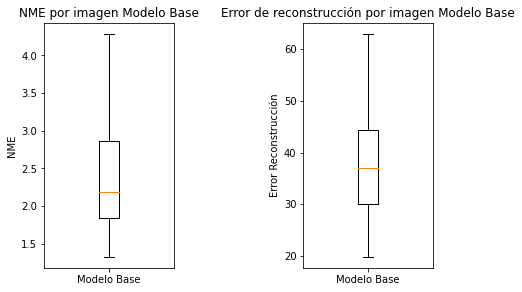
\includegraphics[width=0.9\textwidth]{img/boxplot_modelo_base.png}
            \caption{Diagramas de cajas de los resultados de NME y error de validación en el conjunto de las imágenes de entrenamiento en el Modelo Base. Se han omitido los valores atípicos para una correcta visualización.}
            \label{fig:boxplot_ModeloBase_NME}
        \end{figure}

        \noindent Podemos concluir, que la reconstrucción a nivel de pixel no es adecuada, aunque como vemos en la \autoref{fig:Ejemplo_ModelBase}, la reconstrucción de las caras es apropiada en general, es decir, almacena conocimiento implícito sobre la estructura facial correctamente. Como el framework emplea el conocimiento aprendido sobre la estructura facial para la predicción de landmarks, sería ideal que esta reconstrucción fuese lo más fiel posible. No obstante, el error en el marcado de landmarks cometido es bajo.

        \begin{table}[!ht]
            \centering
            \caption{Media del error NME obtenido por landmark entre todas las particiones de cross-validation. Marcamos en amarillo el vertex pues no está correctamente marcado en todas las imágenes.}
            \begin{tabular}{|l|l|l|}
            \hline
                ~ & \cellcolor{gray!25}\textbf{Landmark} & \cellcolor{gray!25}\textbf{Media NME} \\ \hline
                0 & Menton & 4.176 \\ \hline
                1 & Gnathion & 2.629 \\ \hline
                2 & Pogonion & 2.509 \\ \hline
                3 & Prosthion & 1.178 \\ \hline
                4 & Labiale Superius & 1.965 \\ \hline
                5 & Subnasale & 2.056 \\ \hline
                6 & Nasion & 2.211 \\ \hline
                7 & Glabella & 2.562 \\ \hline
                \cellcolor{yellow!50}8 & \cellcolor{yellow!50}Vertex & \cellcolor{yellow!50}5.904 \\ \hline
                9 & Left Gonion & 5.652 \\ \hline
                10 & Right Gonion & 5.655 \\ \hline
                11 & Left Zygion & 5.351 \\ \hline
                12 & Right Zygion & 6.504 \\ \hline
                13 & Left Alare & 1.972 \\ \hline
                14 & Right Alare & 2.27 \\ \hline
                15 & Left Endocanthion & 1.675 \\ \hline
                16 & Right Endocanthion & 1.731 \\ \hline
                17 & Left Exocanthion & 1.7 \\ \hline
                18 & Right Exocanthion & 1.651 \\ \hline
                19 & Left Tragion & 4.15 \\ \hline
                20 & Right Tragion & 5.639 \\ \hline
                21 & Labiale inferius & 1.734 \\ \hline
                22 & Trichion & 4.445 \\ \hline
                23 & Supramentale & 1.933 \\ \hline
                24 & Left Frontotemporale & 2.37 \\ \hline
                25 & Right Frontotemporale & 2.97 \\ \hline
                26 & Left Frontozygomaticus & 1.566 \\ \hline
                27 & Right Frontozygomaticus & 2.483 \\ \hline
                28 & Left Midsurpaorbital & 1.168 \\ \hline
                29 & Right Midsupraorbital & 1.429 \\ \hline
            \end{tabular}
            \label{table:ModelBase_landmarkresume}
        \end{table}
        \medskip

        \noindent Los resultados por landmark se puden ver en la \autoref{table:ModelBase_landmarkresume} y son buenos en general para tratarse del modelo base. El landmark mejor marcado en media es el \textit{Prosthion}, y el peor el \textit{Right Zygion}. Si recordamos la \autoref{fig:Histograma}, sorprende el hecho de que el \textit{Prosthion} es de los landmarks que menos presencia tiene en las imágenes (aparece en menos de $40$ imágenes), esto nos demuestra la capacidad de 3FabRec de aprender con pocos ejemplos de entrenamiento. Por otro lado, el \textit{Right Zygion}, pese a aparecer en unas $100$ imágenes, resulta más dificil para la red predecirlo. Esto puede deberse a que las imágenes con mayor error de reconstrucción son las de perfil, y es en este tipo de imágenes en las que mejor se aprecia dicho landmark. Por otro lado, pese a que el \textit{Vertex} no se encuentra correctamente marcado en la mayoría de las imágenes, hemos optado por medir su rendimiento también.

        \medskip

        \noindent En la \autoref{fig:Curvas_modelbase} podemos observar las curvas de aprendizaje de cada partición. Podemos observar un rápido descenso del error en entrenamiento y validación hasta la época $30$-$40$, a partir de la cual tiende a estabilizarse el error.

        \begin{figure}[H]
            \centering
            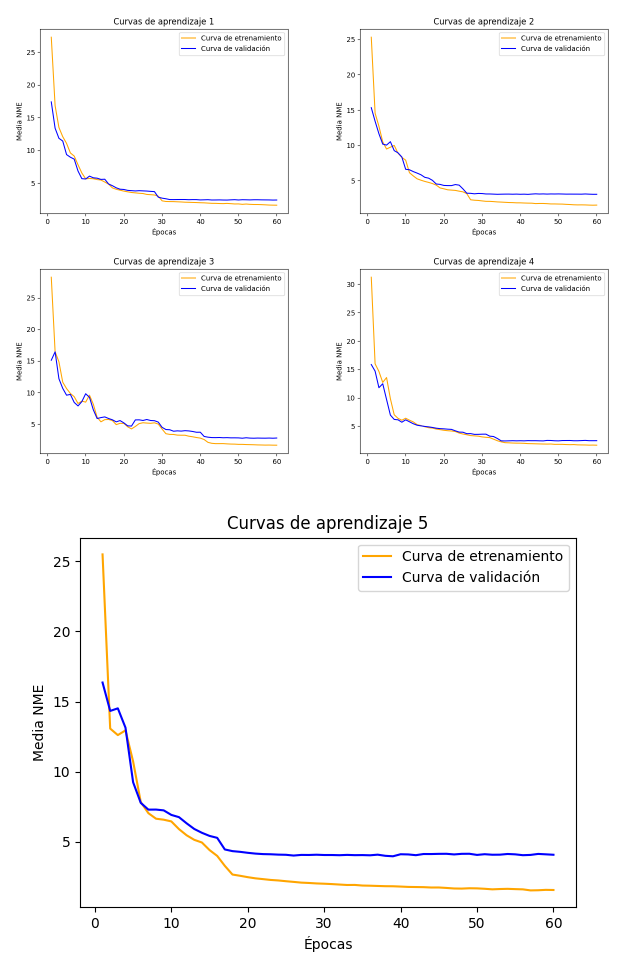
\includegraphics[width=0.9\textwidth]{img/curvas_aprendizaje_modelbase.png}
            \caption{Curvas de aprendizaje en cada partición del modelo base.}
            \label{fig:Curvas_modelbase}
        \end{figure}

        \noindent En resumen, los resultados son esperanzadores para tratarse de una primera aproximación. Sin embargo, consideramos que debido a la gran variabilidad del dataset tanto en posturas, como en calidad e iluminación de imagen, la reconstrucción de las imágenes se ha resentido, especialmente en las imágenes de perfil. Esto provoca que el modelo también marque peor los landmarks, por lo que vamos a intentar mejorar esto en los próximos modelos. 
        
        
        \subsubsection*{Análisis cualitativo}
        
        \medskip Podemos ver el rendimiento del modelo en algunas imágenes en la \autoref{fig:Ejemplo_ModelBase}, en ellas podemos apreciar algunos ejemplos a color y en escalas de grises. Como podemos apreciar, los errores más altos de reconstrucción se producen en las imágenes en escalas de grises y con menor calidad, mientras que los errores más bajos se producen en las imágenes a color, que por lo general tiene mayor resolución. Por otro lado, se puede apreciar que el error cometido por el modelo es bajo en todos los casos, aunque como anticipamos en la sección anterior, el \textit{Vertex} apenas se aprecia en ningún ejemplo.

        \begin{figure}[H]
            \centering
            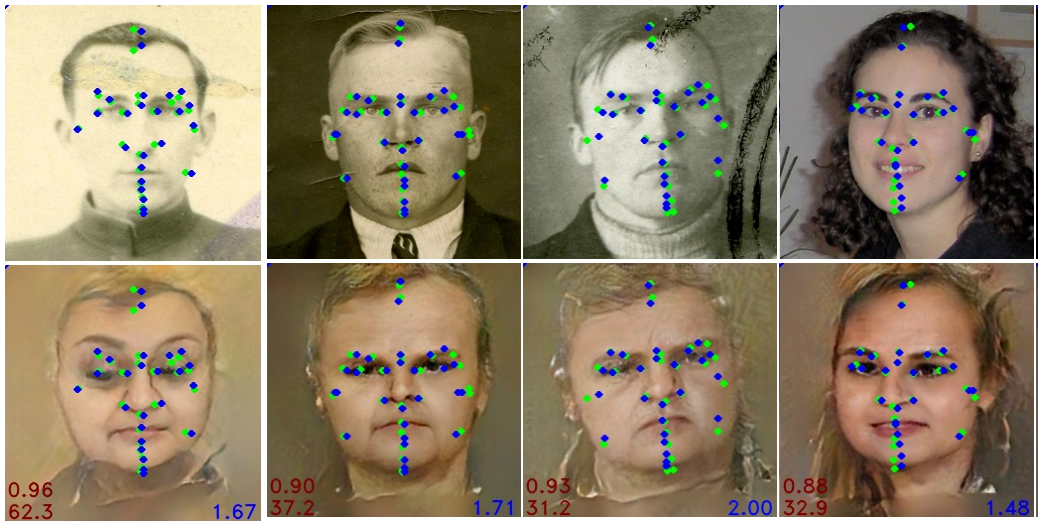
\includegraphics[width=0.9\textwidth]{img/image_basemodel.png}
            \caption{Imágenes pertenecientes a distintos conjuntos de validación para el \textbf{modelo base}. Las imágenes de la fila superior son las imágenes reales, y las de la fila inferior las reconstruidas por la red. El marcado se realiza sobre las reconstruidas y luego se lleva a las superiores. Podemos apreciar en verde los landmarks reales y  en azul los predichos. El valor que aparece en la esquina inferior derecha es el NME global de la imagen (la media de los NMEs de cada landmark) y en la esquina inferior izquierda aparece el error de reconstrucción y encima el SSIM.}
            \label{fig:Ejemplo_ModelBase}
        \end{figure}

    \subsection{Modelo con reentrenamiento del encoder}
        \noindent A la luz de los resultados anteriores, vamos a cambiar el modelo de para entrenar las ITLs (que seguirán usando el mismo optimizador con los mismos parámetros por defecto), junto con los pesos del \textit{encoder}. Con este enfoque, se pretende asociar a cada imagen un vector latente que capte las nuevas variaciones del dataset junto con el entrenamiento en la predicción de landmarks.

        \medskip

        \noindent Este proceso restringe el riesgo de producir \textit{overfitting}, pues durante las etapas de entrenamiento los pesos del \textit{decoder} permanecerán congelados, y serán únicamente los pesos del \textit{encoder} y las ITLs los que se actualicen con backpropagation. El optimizador empleado para el entrenamiento del \textit{encoder} es Adam, junto con sus parámetros por defecto $\beta_1=0.9$ y $\beta_2=0.999$. El \textit{learning rate} se establece a $2^{-6}$, en vez de $2^{-5}$ pues, durante la experimentación, el antiguo \textit{learning rate} quedaba atrapado en extremos locales con facilidad. El entrenamiento duró en total \textbf{100 épocas}, pues como veremos, el modelos mejora más lentamente en el reconocimiento de landmarks.

        \subsubsection*{Análisis Cuantitativo}

        \noindent Como podemos ver en la \autoref{table:ModelEncoder_images_results} y la \autoref{fig:boxplot_ModeloEncoder_NME}, la distribución de los errores de reconstrucción y NME es prácticamente idéntica a la anterior, con la única salvedad de que se ha reducido el número de outliers en una unidad. Las tablas con las predicciones por imagen pueden consultarse en el \autoref{ap:apendiceB}.

        \begin{table}[!ht]
            \centering
            \caption{Métricas obtenidas de la distribución de los errores cometidos en el conjunto de entrenamiento con el modelo de ajuste fino del encoder.}
            \begin{tabular}{|l|l|l|l|l|l|l|}
            \hline
            \cellcolor{gray!25}\textbf{Error} & \cellcolor{gray!25}\textbf{P25} & \cellcolor{gray!25}\textbf{P50} & \cellcolor{gray!25}\textbf{P75} & \cellcolor{gray!25}\textbf{RI} & \cellcolor{gray!25}\textbf{Media} & \cellcolor{gray!25}\textbf{Valores atípicos}\\ \hline
                NME & 1.804 & 2.163 & 2.912 & 1.107 & 2.978 & 11 \\ \hline
                Reconstrucción & 30.128 & 37.225 & 44.1135 & 13.98 & 38.006 & 3 \\ \hline
            \end{tabular}
            \label{table:ModelEncoder_images_results}
        \end{table}

        \begin{figure}[H]
            \centering
            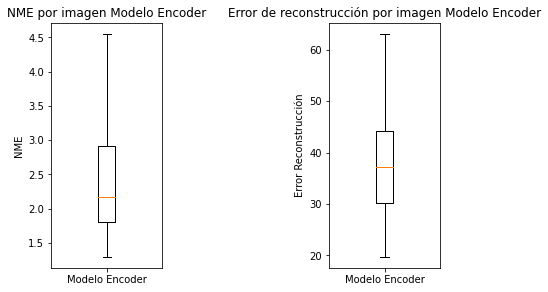
\includegraphics[width=0.9\textwidth]{img/boxplot_encoder.png}
            \caption{Diagramas de cajas de los resultados de NME y error de validación en el conjunto de las imágenes de entrenamiento del modelo de ajuste fino del encoder. Se han omitido los Outliers para una correcta visualización.}
            \label{fig:boxplot_ModeloEncoder_NME}
        \end{figure}

        \begin{table}[!ht]
            \centering
            \caption{Tabla comparativa entre los dos modelos explorados por ahora. Medimos el NME medio a nivel de landmark. En verde se resalta el mejor valor de marcado para cada landmark.}
            \begin{tabular}{|l|l|l|}
            \hline
            \cellcolor{gray!25}\textbf{Landmark} & \cellcolor{gray!25}\textbf{M. Base} & \cellcolor{gray!25}\textbf{M. Encoder} \\ \hline
                Menton & 4.176 & \cellcolor{green!25}3.997 \\ \hline
                Gnathion & 2.629 & \cellcolor{green!25}2.606 \\ \hline
                Pogonion & \cellcolor{green!25}2.509 & 2.546 \\ \hline
                Prosthion & 1.178 & \cellcolor{green!25}1.048 \\ \hline
                Labiale Superius & \cellcolor{green!25}1.965 & 2.04 \\ \hline
                Subnasale & 2.056 & \cellcolor{green!25}1.992 \\ \hline
                Nasion & 2.211 & \cellcolor{green!25}2.099 \\ \hline
                Glabella & \cellcolor{green!25}2.562 & 2.736 \\ \hline
                \cellcolor{yellow!50}Vertex &\cellcolor{yellow!50} 5.904 & \cellcolor{yellow!50}5.89 \\ \hline
                Left Gonion & \cellcolor{green!25}5.652 & 5.789 \\ \hline
                Right Gonion & 5.655 & \cellcolor{green!25}5.301 \\ \hline
                Left Zygion & 5.351 & \cellcolor{green!25}5.288 \\ \hline
                Right Zygion & 6.504 & \cellcolor{green!25}6.291 \\ \hline
                Left Alare & 1.972 & \cellcolor{green!25}1.959 \\ \hline
                Right Alare & 2.27 & \cellcolor{green!25}2.232 \\ \hline
                Left Endocanthion & \cellcolor{green!25}1.675 & 1.71 \\ \hline
                Right Endocanthion & 1.731 & \cellcolor{green!25}1.647 \\ \hline
                Left Exocanthion & \cellcolor{green!25}1.7 & 1.733 \\ \hline
                Right Exocanthion & \cellcolor{green!25}1.651 & 1.746 \\ \hline
                Left Tragion & 4.15 & \cellcolor{green!25}3.633 \\ \hline
                Right Tragion & 5.639 & \cellcolor{green!25}5.252 \\ \hline
                Labiale inferius & 1.734 & \cellcolor{green!25}1.688 \\ \hline
                Trichion & \cellcolor{green!25}4.445 & 4.762 \\ \hline
                Supramentale & \cellcolor{green!25}1.933 & 1.991 \\ \hline
                Left Frontotemporale & \cellcolor{green!25}2.37 & 2.452 \\ \hline
                Right Frontotemporale & \cellcolor{green!25}2.97 & 3.282 \\ \hline
                Left Frontozygomaticus & 1.566 & \cellcolor{green!25}1.499 \\ \hline
                Right Frontozygomaticus & \cellcolor{green!25}2.483 & 2.516 \\ \hline
                Left Midsurpaorbital & \cellcolor{green!25}1.168 & 1.178 \\ \hline
                Right Midsupraorbital & 1.429 & \cellcolor{green!25}1.348 \\ \hline
            \end{tabular}
            \label{table:Encode_landmarkresume}
        \end{table}

    \noindent Como podemos observar en la \autoref{table:Encode_landmarkresume}, los valores son muy similares a los del modelo base, pese a que este ha entrenado durante más épocas. El \textit{Prosthion} sigue siendo el landmark mejor marcado, con un valor del error NME ligeramente inferior al del modelo base. Se puede apreciar una mejora en los landmarks peor marcados, todos ellos asociados a los laterales del rostro y con mayor presencia en imágenes de perfil. Esto confirma la relación entre la mejora de la reconstrucción en imágenes de perfil y el NME asociado a los landmarks de las mismas.
    

    \medskip

    \noindent Finalmente podemos observar las curvas de aprendizaje para este modelo en la \autoref{fig:curvas_encoder}. A diferencia del modelo anterior, comienza a bajar la capacidad de generalización a partir de la época $20$-$30$ aproximadamente. El error de entrenamiento comienza a descender muy lentamente con cada época mientras que el de validación se mantiene constante.

    \begin{figure}[H]
        \centering
        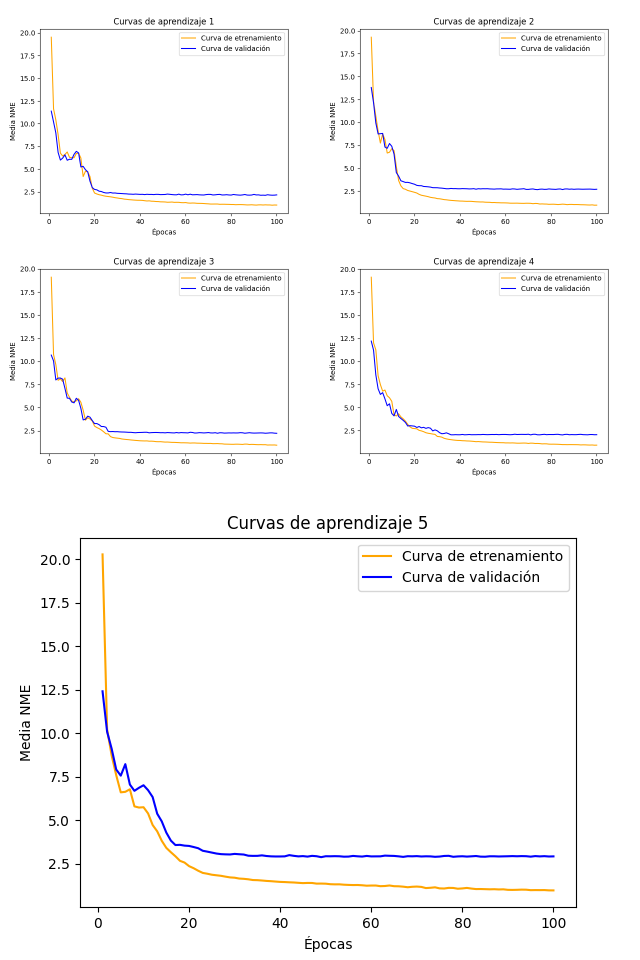
\includegraphics[width=0.9\textwidth]{img/curvas_encoder.png}
        \caption{Curvas de aprendizaje en cada partición del modelo de finetuning del encoder.}
        \label{fig:curvas_encoder}
    \end{figure}

    \medskip

    \noindent Viendo estos resultados, no parece muy prometedora esta línea de investigación. Bien es cierto que hemos mejorado el error de los dos landmarks peor marcados, pero el coste computacional que ha supuesto no compensa para la leve mejora global del modelo. Es por esto por lo que vamos a cambiar el enfoque sobre el \textit{fine-tuning} en el siguiente modelo. 
    
    \medskip
    
    \noindent No obstante, consideramos que un reentrenamiento de los pesos del \textit{AAE} en la fase de aprendizaje no supervisado con imágenes complicadas en escalas de grises y de perfil habría sido una buena alternativa, pero lamentablemente no disponemos de los datos necesarios para realizar este eperimento.
    
    
    \subsubsection*{Análisis Cualitativo}
    
    \noindent Podemos ver el comportamiento del modelo en algunas imágenes de validación de diversas particiones de \textit{cross-validation} en la \autoref{fig:Ejemplo_encoder}. Se puede ver una leve mejora del error de reconstrucción con respecto a las imágenes del modelo anterior. No obstante a nivel visual apenas se notan diferencias significativas tanto en el marcado de los landmarks como en la reconstrucción de las imágenes.

    \begin{figure}[H]
        \centering
        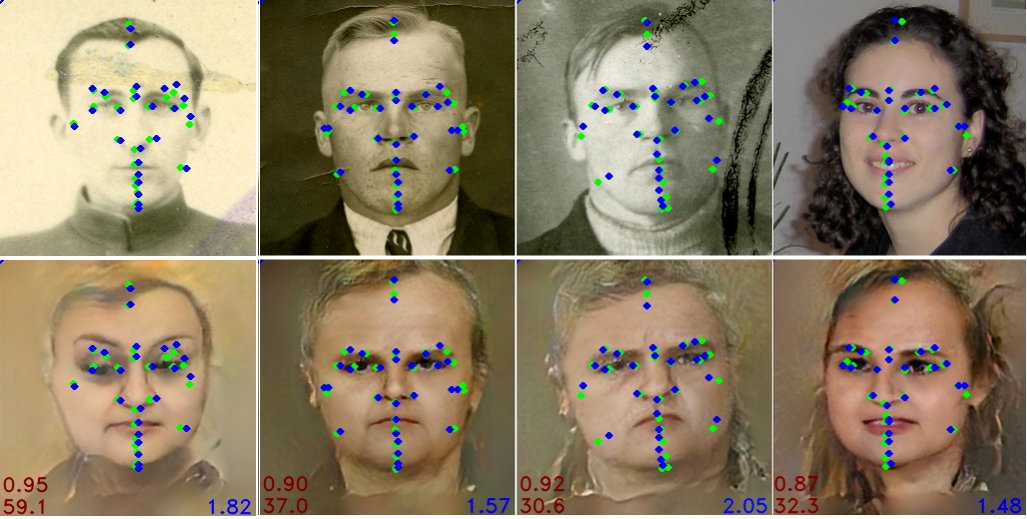
\includegraphics[width=0.9\textwidth]{img/image_encoder.png}
        \caption{Imágenes pertenecientes a distintos conjuntos de validación para el \textbf{modelo de ajuste fino del encoder}.}
        \label{fig:Ejemplo_encoder}
    \end{figure}

    \subsection{Modelo con reentrenamiento del decoder}
        \noindent Del mismo modo en que se experimentó con el \textit{encoder} se hizo con el \textit{decoder}. En este enfoque asumimos que el framework sabe codificar correctamente las imágenes pero que no realiza lo suficientemente bien la reconstrucción de las mismas debido a la alta variabilidad del dataset. Esta etapa es completamente análoga a la del modelo anterior (incluyendo el mismo tipo de optimizadores, parámetros y regiones que permanecen congeladas de la red), pero actualizando los pesos del \textit{decoder} y las ITLs mientras se congelan los pesos del \textit{encoder}.

        \subsubsection*{Análisis Cuantitativo}

        \noindent Podemos observar los resultados obtenidos en la \autoref{fig:boxplot_ModeloDecoder_NME} y la \autoref{table:ModelDecoder_images_results}. Los resultados son muy similares a los anteriores modelos e incluso empeoran ligeramente en el marcado de landmarks, aumentando el número de outliers en la distribución de los errores NME a 13. Las tablas por partición se pueden consultar en \autoref{ap:apendiceC}.

    \begin{table}[!ht]
            \centering
            \caption{Métricas obtenidas de la distribución de los errores cometidos en el conjunto de entrenamiento con el modelo de ajuste fino del decoder.}
            \begin{tabular}{|l|l|l|l|l|l|l|}
            \hline
            \cellcolor{gray!25}\textbf{Error} & \cellcolor{gray!25}\textbf{P25} & \cellcolor{gray!25}\textbf{P50} & \cellcolor{gray!25}\textbf{P75} & \cellcolor{gray!25}\textbf{RI} & \cellcolor{gray!25}\textbf{Media} & \cellcolor{gray!25}\textbf{Valores atípicos}\\ \hline
                NME & 1.868 & 2.249 & 2.925 & 1.057 & 3.039 & 13 \\ \hline
                Reconstrucción & 30.02 & 37.104 & 44.382 & 14.357 & 38.043 & 3 \\ \hline
            \end{tabular}
            \label{table:ModelDecoder_images_results}
        \end{table}

        \begin{figure}[H]
            \centering
            \includegraphics[width=0.9\textwidth]{img/boxplot_decoder.png}
            \caption{Diagramas de cajas de los resultados de NME y error de validación en el conjunto de las imágenes de entrenamiento del modelo de ajuste fino del decoder. Se han omitido los Outliers para una correcta visualización.}
            \label{fig:boxplot_ModeloDecoder_NME}
        \end{figure}

        \begin{table}[!ht]
            \centering
            \caption{Tabla comparativa entre los tres modelos probados. En este caso no se aprecia ninguna mejora considerable con respecto a las introducidas por el modelo de ajuste fino del encoder.}
            \begin{tabular}{|l|l|l|l|}
            \hline
                \cellcolor{gray!25}\textbf{Landmark} & \cellcolor{gray!25}\textbf{M. Base} & \cellcolor{gray!25}\textbf{M. Encoder} & \cellcolor{gray!25}\textbf{M. Decoder} \\ \hline
                Menton & 4.176 & 3.997 & \cellcolor{green!25}3.991 \\ \hline
                Gnathion & 2.629 &  \cellcolor{green!25}2.606 & 2.634 \\ \hline
                Pogonion &  \cellcolor{green!25}2.509 & 2.546 & 2.585 \\ \hline
                Prosthion & 1.178 &  \cellcolor{green!25}1.048 & 0.97 \\ \hline
                Labiale Superius &  \cellcolor{green!25}1.965 & 2.04 & 2.059 \\ \hline
                Subnasale & 2.056 &  \cellcolor{green!25}1.992 & 2.089 \\ \hline
                Nasion & 2.211 &  \cellcolor{green!25}2.099 & 2.275 \\ \hline
                Glabella & 2.562 &  \cellcolor{green!25}2.736 & 2.912 \\ \hline
                \cellcolor{yellow!50}Vertex &\cellcolor{yellow!50} 5.904 &  \cellcolor{yellow!50}5.89 & \cellcolor{yellow!50}6.137 \\ \hline
                Left Gonion & \cellcolor{green!25}5.652 & 5.789 & 5.665 \\ \hline
                Right Gonion & 5.655 & \cellcolor{green!25}5.301 & 5.468 \\ \hline
                Left Zygion & 5.351 & \cellcolor{green!25}5.288 & 5.29 \\ \hline
                Right Zygion & 6.504 & 6.291 & \cellcolor{green!25}6.14 \\ \hline
                Left Alare & 1.972 & \cellcolor{green!25}1.959 & 2.051 \\ \hline
                Right Alare & 2.27 & \cellcolor{green!25}2.232 & 2.295 \\ \hline
                Left Endocanthion & \cellcolor{green!25}1.675 & 1.71 & 1.827 \\ \hline
                Right Endocanthion & 1.731 & 1.647 & \cellcolor{green!25}1.61 \\ \hline
                Left Exocanthion & \cellcolor{green!25}1.7 & 1.733 & 1.809 \\ \hline
                Right Exocanthion & \cellcolor{green!25}1.651 & 1.746 & 1.734 \\ \hline
                Left Tragion & 4.15 & \cellcolor{green!25}3.633 & 4.163 \\ \hline
                Right Tragion & 5.639 & 5.252 & \cellcolor{green!25}4.791 \\ \hline
                Labiale inferius & 1.734 & 1.688 & \cellcolor{green!25}1.627 \\ \hline
                Trichion & \cellcolor{green!25}4.445 & 4.762 & 5.196 \\ \hline
                Supramentale & 1.933 & 1.991 & \cellcolor{green!25}1.839 \\ \hline
                Left Frontotemporale & \cellcolor{green!25}2.37 & 2.452 & 2.474 \\ \hline
                Right Frontotemporale & \cellcolor{green!25}2.97 & 3.282 & 3.009 \\ \hline
                Left Frontozygomaticus & 1.566 & \cellcolor{green!25}1.499 & 1.525 \\ \hline
                Right Frontozygomaticus & 2.483 & 2.516 & \cellcolor{green!25}2.395 \\ \hline
                Left Midsurpaorbital & \cellcolor{green!25}1.168 & 1.178 & 1.191 \\ \hline
                Right Midsupraorbital & 1.429 & \cellcolor{green!25}1.348 & 1.48 \\ \hline
            \end{tabular}
            \label{table:Decoder_landmarksresume}
        \end{table}
        \medskip 

        \noindent De nuevo los errores por landmark que se muestran en la tabla \autoref{table:Decoder_landmarksresume} es muy similar a la de los dos modelos anteriores, por lo que no hemos logrado una gran mejora con este modelo tampoco.

        \medskip

        \noindent Las curvas de aprendizaje se pueden ver en la \autoref{fig:curvas_decoder}, y vuelven a mostrar un ligero overfitting a partir de la época $30$-$40$, en la mayoría de casos. 
        
        \begin{figure}[H]
            \centering
            \includegraphics[width=0.9\textwidth]{img/curvas_decoder.png}
            \caption{Curvas de aprendizaje en cada partición del modelo de finetuning del encoder.}
            \label{fig:curvas_decoder}
        \end{figure}

        \medskip

        \noindent Tras los resultados obtenidos se ha optado por abandonar también esta línea de investigación pues se obtienen resultados muy similares al modelo base y se debe entrenar por mucho más tiempo ($100$ épocas frente a $40$ del modelo base). 
        
        \subsubsection*{Análisis Cualitativo}
        
        Los resultados del modelo sobre algunas imágenes pueden verse en \autoref{fig:Ejemplo_decoder}. Las conclusiones a extraer son las mismas que en el modelo anterior: Apenas mejora el error de reconstrucción (incluso empeora en el caso de la imagen a color), y no se aprecian diferencias significativas en el marcado de landmarks con respecto a los modelos anteriores.

        \begin{figure}[H]
            \centering
            \includegraphics[width=0.9\textwidth]{img/image_decoder.png}
            \caption{Imágenes pertenecientes a distintos conjuntos de validación para el \textbf{modelo de ajuste fino del decoder}.}
            \label{fig:Ejemplo_decoder}
        \end{figure}

    \subsection{Modelo con Data Augmentation}
        \noindent Vamos a optar a continuación por un nuevo enfoque. En lugar de mejorar el error de reconstrucción, vamos a centrarnos en mejorar el marcado de landmarks en las imágenes reconstruidas que genera el modelo preentrenado. Como pudimos ver en el modelo base, se consiguieron buenos resultados del \textit{NME} pese a haber entrenado sin realizar técnicas de \textit{data augmentation}. Es por ello que en este segundo experimento vamos a realizar los siguientes cambios en el entrenamiento: 
        
        \begin{itemize}
            \item Se realizará un entrenamiento del modelo similar al del modelo base durante $40$ épocas, ya que vimos que el error convergía tras la época 40.
            \item Tras esto, se entrenará el modelo con el dataset al cual se le aplicarán técnicas de data augmentation, para aumentar el número de datos de entrenamiento e incrementar aún más la variabilidad de los mismos, de manera que cada imagen del dataset sufrirá de manera aleatoria una traslación ($\pm 4\%$), un reescalado ($\pm 5\%$), una rotación ($\pm 30$ grados) y oclusiones parciales. El entrenamiento en este nuevo dataset será durante $40$ épocas tras acabar las de la etapa anterior.
            \item En total serán \textbf{$80$ épocas} de entrenamiento sumando las dos etapas anteriores.
        \end{itemize}

        \medskip

        \noindent De nuevo, el resto de parámetros continuarán con los valores por defecto de la etapa anterior, pues los resultados obtenidos han sido buenos hasta el momento y nada sugiere tener que cambiarlos.

        \medskip

        \noindent Los resultados por imagen de \textbf{cross-validation}, pueden consultarse en la \autoref{table:ModelDaug_images_results} y la \autoref{fig:boxplot_ModeloDaug_NME}. En este caso, se aprecia una considerable mejora en el error del NME, compactando mucho la distribución, como vemos, el rango intercuartílico (RI) es de $0,371$. Los valores atípicos suben a los $13$, lo que suponen un $10\%$ de los datos aproximadamente. No obstante, podemos concluir que le modelo es robusto, a pesar de la gran variabilidad de los datos empleados. Por otro lado, la distribución del error de reconstrucción es idéntica a la del modelo base, ya que no entrenamos los pesos del encoder ni decoder.

        \begin{table}[!ht]
            \centering
            \caption{Métricas obtenidas de la distribución de los errores cometidos en el conjunto de entrenamiento con el modelo de data augmentation.}
            \begin{tabular}{|l|l|l|l|l|l|l|}
            \hline
            \cellcolor{gray!25}\textbf{Error} & \cellcolor{gray!25}\textbf{P25} & \cellcolor{gray!25}\textbf{P50} & \cellcolor{gray!25}\textbf{P75} & \cellcolor{gray!25}\textbf{RI} & \cellcolor{gray!25}\textbf{Media} & \cellcolor{gray!25}\textbf{Valores atípicos}\\ \hline
                NME & 1.1 & 1.253 & 1.472 & 0.371 & 1.706 & 13 \\ \hline
                Reconstrucción & 30.024 & 37.104 & 44.382 & 14.357 & 38.043 & 3 \\ \hline
            \end{tabular}
            \label{table:ModelDaug_images_results}
        \end{table}

        \begin{figure}[H]
            \centering
            \includegraphics[width=0.9\textwidth]{img/boxplot_daug.png}
            \caption{Diagramas de cajas de los resultados de NME y error de validación en el conjunto de las imágenes de entrenamiento del modelo de data augmentation. Se han omitido los Outliers para una correcta visualización.}
            \label{fig:boxplot_ModeloDaug_NME}
        \end{figure}

        \begin{table}[!ht]
            \centering
            \caption{Tabla comparativa entre todos los modelos probados.}
            \begin{tabular}{|l|l|l|l|l|}
            \hline
                \cellcolor{gray!25}\textbf{Landmark} & \cellcolor{gray!25}\textbf{M. Base} & \cellcolor{gray!25}\textbf{M. Encoder} & \cellcolor{gray!25}\textbf{M. Decoder} & \cellcolor{gray!25}\textbf{M. Data Augmentation} \\ \hline
                Menton & 4.176 & 3.997 & 3.991 & \cellcolor{green!25}3.006 \\ \hline
                Gnathion & 2.629 & 2.606 & 2.634 & \cellcolor{green!25}1.497 \\ \hline
                Pogonion & 2.509 & 2.546 & 2.585 & \cellcolor{green!25}1.359 \\ \hline
                Prosthion & 1.178 & 1.048 & 0.97 & \cellcolor{green!25}0.815 \\ \hline
                Labiale Superius & 1.965 & 2.04 & 2.059 & \cellcolor{green!25}1.531 \\ \hline
                Subnasale & 2.056 & 1.992 & 2.089 & \cellcolor{green!25}1.272 \\ \hline
                Nasion & 2.211 & 2.099 & 2.275 & \cellcolor{green!25}1.241 \\ \hline
                Glabella & 2.562 & 2.736 & 2.912 & \cellcolor{green!25}1.545 \\ \hline
                \cellcolor{yellow!50}Vertex & \cellcolor{yellow!50}5.904 & \cellcolor{yellow!50}5.89 & \cellcolor{yellow!50}6.137 & \cellcolor{yellow!50}3.99 \\ \hline
                Left Gonion & 5.652 & 5.789 & 5.665 & \cellcolor{green!50}1.846 \\ \hline
                Right Gonion & 5.655 & 5.301 & 5.468 & \cellcolor{green!50}1.673 \\ \hline
                Left Zygion & 5.351 & 5.288 & 5.29 & \cellcolor{green!50}3.322 \\ \hline
                Right Zygion & 6.504 & 6.291 & 6.14 & \cellcolor{green!50}4.441 \\ \hline
                Left Alare & 1.972 & 1.959 & 2.051 & \cellcolor{green!25}1.585 \\ \hline
                Right Alare & 2.27 & 2.232 & 2.295 & \cellcolor{green!25}1.362 \\ \hline
                Left Endocanthion & 1.675 & 1.71 & 1.827 & \cellcolor{green!25}1.227 \\ \hline
                Right Endocanthion & 1.731 & 1.647 & 1.61 & \cellcolor{green!25}1.129 \\ \hline
                Left Exocanthion & 1.7 & 1.733 & 1.809 & \cellcolor{green!25}1.186 \\ \hline
                Right Exocanthion & 1.651 & 1.746 & 1.734 & \cellcolor{green!25}1.12 \\ \hline
                Left Tragion & 4.15 & 3.633 & 4.163 & \cellcolor{green!25}2.066 \\ \hline
                Right Tragion & 5.639 & 5.252 & 4.791 & \cellcolor{green!25}2.234 \\ \hline
                Labiale inferius & 1.734 & 1.688 & 1.627 & \cellcolor{green!25}1.032 \\ \hline
                Trichion & 4.445 & 4.762 & 5.196 & \cellcolor{green!25}3.37 \\ \hline
                Supramentale & 1.933 & 1.991 & 1.839 & \cellcolor{green!25}1.109 \\ \hline
                Left Frontotemporale & 2.37 & 2.452 & 2.474 & \cellcolor{green!25}1.386 \\ \hline
                Right Frontotemporale & 2.97 & 3.282 & 3.009 & \cellcolor{green!25}1.826 \\ \hline
                Left Frontozygomaticus & 1.566 & 1.499 & 1.525 & \cellcolor{green!25}1.036 \\ \hline
                Right Frontozygomaticus & 2.483 & 2.516 & 2.395 & \cellcolor{green!25}1.057 \\ \hline
                Left Midsurpaorbital & 1.168 & 1.178 & 1.191 &\cellcolor{green!25} 0.854 \\ \hline
                Right Midsupraorbital & 1.429 & 1.348 & 1.48 & \cellcolor{green!25}0.945 \\ \hline
            \end{tabular}
            \label{table:Daugmentation_landmarksresume}
        \end{table}

        \medskip

        \noindent Como podemos ver en la \autoref{table:Daugmentation_landmarksresume}, los errores se han reducido en todos los landmarks. Además, la red ha conseguido aprender a marcar con un alto grado de precisión los puntos que se ven en el perfil, siendo esta alternativa menos costosa que la de los dos modelos anteriores tanto en número de épocas como en parámetros que se actualizan de la red (en este nuevo modelo sólo se actualizan los pesos de las ITLs). El punto mejor marcado sería el \textit{prosthion} de nuevo, y el peor marcado el \textit{right zygion}. Sin embargo, la diferencia en términos de error entre ambos es mucho menor que en el caso del modelo base. 

        
        \subsubsection*{Análisis Cualitativo}
        \noindent Finalmente las curvas de aprendizaje obtenidas se pueden observar en \autoref{fig:curvas_daugmentation}. Como vemos presentan una gran capacidad de generalización, pues el error de entrenamiento y validación decrecen de forma continua y muy próxima. Algunas imágenes de ejemplo podemos verlas en la \autoref{fig:Ejemplo_daug}.

        \begin{figure}[H]
            \centering
            \includegraphics[width=0.9\textwidth]{img/curvas_daugmentation.png}
            \caption{Curvas de aprendizaje en cada partición del modelo de data augmentation.}
            \label{fig:curvas_daugmentation}
        \end{figure}

        \begin{figure}[H]
            \centering
            \includegraphics[width=0.9\textwidth]{img/image_daug.png}
            \caption{Imágenes pertenecientes a distintos conjuntos de validación para el \textbf{modelo data augmentation}.}
            \label{fig:Ejemplo_daug}
        \end{figure}

    \subsection{Elección de modelo y obtención de resultados}

        \noindent Una vez analizados los distintos modelos que se proponen para resolver el problema, vemos que la alternativa más prometedora resulta ser la última. Podemos ver una comparación de la distribución de los errores de NME y reconstrucción de todos los modelos en la \autoref{fig:boxplot_summary}, aquí podemos ver mejor la gran reducción del error NME lograda por el último modelo. Por otro lado, la distribución de los errores de reconstrucción apenas varía en los cuatro modelos probados. 
        

        \begin{figure}[H]
            \centering
            \includegraphics[width=0.9\textwidth]{img/boxplot_sumarize.png}
            \caption{Diagramas de cajas de todos los modelos probados concatenados. Para una correcta visualización se eliminan los outliers del gráfico.}
            \label{fig:boxplot_summary}
        \end{figure}

        
        \subsubsection*{Análisis Cuantitativo}
        

        \noindent Una vez elegido el modelo, tomamos el conjunto de entrenamiento en su totalidad (sin realizar particiones) y vamos a usarlo para entrenar el modelo durante las mismas épocas que en la sección anterior y con los mismos parámetros y transformaciones. Posteriormente usaremos el conjunto de test de $32$ imágenes que separamos al principio de esta sección, y que hasta ahora no hemos visto para evitar \textit{data snooping}, para validar el modelo.


        \begin{table}[!ht]
            \centering
            \caption{Tabla comparativa entre los resultados del modelo de data augmentation en el conjunto de validación y test.}
            \begin{tabular}{|l|l|l|}
            \hline
                \cellcolor{gray!25}\textbf{Landmark} & \cellcolor{gray!25}\textbf{NME Test} & \cellcolor{gray!25}\textbf{NME Validación} \\ \hline
                \textbf{Menton} & \cellcolor{green!25}0.929 & 3.006 \\ \hline
                \textbf{Gnathion} & \cellcolor{green!25}1.13 & 1.497 \\ \hline
                \textbf{Pogonion} & \cellcolor{green!25}1.262 & 1.359 \\ \hline
                \textbf{Prosthion} & 1.24 & \cellcolor{green!25}0.815 \\ \hline
                \textbf{Labiale Superius} & \cellcolor{green!25}1.135 & 1.531 \\ \hline
                \textbf{Subnasale} & \cellcolor{green!25}0.863 & 1.272 \\ \hline
                \textbf{Nasion} & \cellcolor{green!25}0.871 & 1.241 \\ \hline
                \textbf{Glabella} & \cellcolor{green!25}1.161 & 1.545 \\ \hline
                \textbf{Vertex} & \cellcolor{green!25}2.558 & 3.99 \\ \hline
                \textbf{Left Gonion} & \cellcolor{green!25}1.406 & 1.846 \\ \hline
                \textbf{Right Gonion} & \cellcolor{green!25}1.242 & 1.673 \\ \hline
                \textbf{Left Zygion} & \cellcolor{green!25}1.585 & 3.322 \\ \hline
                \textbf{Right Zygion} & \cellcolor{green!25}1.607 & 4.441 \\ \hline
                \textbf{Left Alare} & \cellcolor{green!25}0.804 & 1.585 \\ \hline
                \textbf{Right Alare} & \cellcolor{green!25}0.835 & 1.362 \\ \hline
                \textbf{Left Endocanthion} & 1.377 & \cellcolor{green!25}1.227 \\ \hline
                \textbf{Right Endocanthion} & 1.656 & \cellcolor{green!25}1.129 \\ \hline
                \textbf{Left Exocanthion} & 1.772 & \cellcolor{green!25}1.186 \\ \hline
                \textbf{Right Exocanthion} & 2.132 & \cellcolor{green!25}1.12 \\ \hline
                \textbf{Left Tragion} & \cellcolor{green!25}1.47 & 2.066 \\ \hline
                \textbf{Right Tragion} & \cellcolor{green!25}1.557 & 2.234 \\ \hline
                \textbf{Labiale inferius} & 1.103 & \cellcolor{green!25}1.032 \\ \hline
                \textbf{Trichion} & \cellcolor{green!25}1.544 & 3.37 \\ \hline
                \textbf{Supramentale} & 1.241 & \cellcolor{green!25}1.109 \\ \hline
                \textbf{Left Frontotemporale} & \cellcolor{green!25}1.293 & 1.386 \\ \hline
                \textbf{Right Frontotemporale} & \cellcolor{green!25}1.17 & 1.826 \\ \hline
                \textbf{Left Frontozygomaticus} & 1.038 & \cellcolor{green!25}1.036 \\ \hline
                \textbf{Right Frontozygomaticus} & \cellcolor{green!25}1.031 & 1.057 \\ \hline
                \textbf{Left Midsurpaorbital} & 0.864 & \cellcolor{green!25}0.854 \\ \hline
                \textbf{Right Midsupraorbital} & 1.92 & \cellcolor{green!25}0.945 \\ \hline
            \end{tabular}
            \label{table:FinalModel_landmarks}
        \end{table}
        
        \medskip

        \noindent En primer lugar, como se puede apreciar en la \autoref{table:FinalModel_landmarks} obtenemos: 

        \begin{itemize}
            \item A primera vista los errores son similares en el conjunto de test que los obtenidos en validación, ligeramente mejores en algunos casos y peores en otros.  
            \item Realizamos un test de \textbf{Kolmogorov-Smirnov} para ver si ambas distribuciones de errores proceden de la misma distribución (que será nuestra hipótesis nula) o no con un $95\%$ de confianza. Para ello empleamos la función \textit{ks\_2samp
            } de la librería \textit{scipy} de python. Esta función nos permite realizar con facilidad el test descrito anteriormente obteniendo un $p-valor=0.594 > 0.05$, por lo que no tenemos evidencias para rechazar la hipótesis nula. Esto es algo deseable, pues los errores de test y validación  deberían seguir la misma distribución.

        \end{itemize}

        \medskip

        \noindent Por otro lado, las curvas de aprendizaje durante el entrenamiento del modelo se pueden observar en la \autoref{fig:curvas_FinalModel}. En ellas podemos observar una gran capacidad de generalización del modelo, pues en todo momento la curva de entrenamiento y la de validación descienden tras cada época y cuando convergen parecen hacerlo al mismo valor. 

        \begin{figure}[H]
            \centering
            \includegraphics[width=0.9\textwidth]{img/curvas_FinalModel.png}
            \caption{Curvas de aprendizaje durante el entrenamiento del modelo de data augmentation validado en el conjunto de test.}
            \label{fig:curvas_FinalModel}
        \end{figure}
        
        \subsubsection*{Análisis Cualitativo}

        \noindent Podemos ver el rendimiento del modelo en algunas imágenes en \autoref{fig:Ejemplo_finalmodel}. Como podemo ver, la reconstrucción de las imágenes continua siendo adecuada y la precisión en el marcado de landmarks es muy elevada. Las imágenes más complicadas siguen siendo las de perfil, debido a la poca calidad de la reconstrucción del \textit{AAE} en este tipo de ejemplos. No obstante, los resultados en global son satisfactorios.

        \begin{figure}[H]
            \centering
            \includegraphics[width=0.9\textwidth]{img/image_finalmodel.png}
            \caption{Rendimiento del modelo final elegido con data augmentation en imágenes del conjunto de test.}
            \label{fig:Ejemplo_finalmodel}
        \end{figure}

        \medskip

        \subsubsection*{Análisis de requisitos}

        \noindent Vamos a ver a continuación si el modelo elegido cumple con los requisitos deseables que nos habíamos impuesto al comienzo del trabajo: 
        \begin{itemize}
            \item Se trata de un modelo \textbf{robusto}, pues tiene un buen comportamiento en la mayoría de ejemplos de test empleados.
            \item Es capaz de operar con un \textbf{pequeño conjunto de datos}, ya que los resultados obtenidos son muy prometedores pese a haber sido entrenado con $131$ imágenes (recordemos que modelos para la predicción de landmarks faciales cuentan con miles de ejemplos de entrenamiento en los datasets).
            \item Proporciona una solución muy próxima a la \textbf{correcta}. Aunque falta la supervisión de un experto antropólogo forense para afirmarlo.
            \item Se trata de un proceso \textbf{eficaz} y \textbf{eficiente}, pues se obtienen buenos resultados en apenas unos segundos de ejecución.
        \end{itemize}

        \medskip

        \noindent Como podemos ver, en general el modelo cumple los requisitos que le habíamos impuesto, y podemos concluir que el modelo resuleve la tarea que nos habíamos propuesto con éxito. No obstante, insistimos en que el éxito real del modelo debe supervisarlo un experto forense, pues no sabemos si los errores cometidos en la identificación de landmarks son errores asumibles o si se requiere un mayor grado de precisión en el marcado.

    \section{Comparativa entre 3FabRec y HyperFace-ResNet101}
        \noindent Vamos a comparar ahora el modelo final obtenido a partir de \textbf{3FabRec} con otro que fue diseñado para el mismo propósito basado en \textbf{HyperFace-Resnet101}, otra red especializada en el marcado de landmarks, realizado por Guillermo Gómez y que supone el estado del arte en el campo.

        \subsection{Preprocesamiento y base de datos empleada}
            \noindent En lo que respecta al preprocesamiento de los datos, nuestro modelo basado en \textit{3FabRec} únicamente emplea como etapa de preprocesamiento la identificación de bounding boxes en el conjunto de datos inicial de cara a poder entrenar la red. Por otro lado, este estudio se limita a usar las $167$ imágenes proporcionadas.

            \medskip

            \noindent En cambio, el modelo basado en \textit{HF-ResNet} además de emplear también un detector de caras para los bounding boxes, contaba con un dataset auxiliar de modelos $3D$ de personas sobre las que estaban marcados $27$ de los $30$ landmarks que se predicen. Lo cual sirvió para aumentar considerablemente el conjunto de datos de entrenamiento realizando proyecciones $2D$ a partir de estos modelos.

        \subsection{Métricas empleadas}
            \noindent La métrica empleada en el trabajo dónde se presenta el modelo es el \textbf{RMSE}. Se trata de la raíz del error cuadrático medio y su expresión es la siguiente: 

            \begin{equation}
                RMSE(y,\widehat{y})= \sqrt{\frac{1}{N} \sum_{i=1}^{N} (y_i-\widehat{y}_i)^2}
            \end{equation}

            \noindent donde $y_i$ representa las coordenadas del landmark real y $\widehat{y_i}$ el predicho homólogo número $i$ del total de $N$ landmarks marcados. Esta métrica nos proporciona el error en píxeles cometido en la predicción de cada landmark.

            \medskip

            \noindent Para poder realizar una comparación entre ambos métodos, se extrae esta métrica del rendimiento del modelo final en el conjunto de test. 

        \subsection{Comparación de resultados}
            \noindent En primer lugar comparamos ambos modelos calculando la mediana del \textit{RMSE} producido en cada landmark, así como los percentiles $25$, $50$ y $75$. Podemos ver estos resultados en la \autoref{table:comparativa-global}.

            \begin{table}[!ht]
                \centering
                \caption{Tabla comparativa a nivel global entre los dos modelos. Como podemos observar, el modelo basado en \textbf{HyperFace-Resnet101} obtiene mejores resultados en global en todos los campos.}
                \begin{tabular}{|l|l|l|l|l|}
                \hline
                    \cellcolor{gray!25}\textbf{Modelo} & \cellcolor{gray!25}\textbf{RMSE} & \cellcolor{gray!25}\textbf{P25} & \cellcolor{gray!25}\textbf{P50} & \cellcolor{gray!25}\textbf{P75} \\ \hline
                    \textbf{Modelo HyperFace-Resnet101} & 3.4106 & \cellcolor{green!25}1.802 & 2.7569 & 4.2849 \\ \hline
                    \textbf{Modelo 3FabRec} & \cellcolor{green!25} 2.7666 & 1.9561 & \cellcolor{green!25}2.3812 & \cellcolor{green!25}3.1201 \\ \hline
                \end{tabular}
                \label{table:comparativa-global}
            \end{table}
            
            \medskip

            \noindent A nivel general, parece que el modelo basado en \textit{3FabRec} es mejor que el basado en \textit{HF-Resnet101}. Como podemos ver en los resultados de la \autoref{table:comparativa-global}, a nivel de distribución del error RMSE en las imágenes de test, el RI en el modelo de \textit{HF-Resnet101} es de $2.48$ píxeles, mientras que en el modelo de \textit{3FabRec} es de $1.164$ píxeles, lo que supone una mejora considerable. No obstante, vamos a realizar una comparativa a nivel de landmark entre los dos modelos. Podemos ver esta comparativa en la \autoref{table:comparativa-Landmarks}.

            \begin{table}[!ht]
                \centering
                \caption{Tabla comparativa a nivel de landmarks entre el modelo final basado en 3FabRec y el de HyperFace-REsNet101.}
                \begin{tabular}{|l|l|l|}
                \hline
                    \cellcolor{gray!25}\textbf{Landmark} & \cellcolor{gray!25}\textbf{RMSE 3FabRec} & \cellcolor{gray!25}\textbf{RMSE HyperFace-Resnet101} \\ \hline
                    \textbf{Menton} & \cellcolor{green!25}1.79 &  4.97 \\ \hline
                    \textbf{Gnathion} & \cellcolor{green!25}2.28 & 3.84 \\ \hline
                    \textbf{Pogonion} & \cellcolor{green!25}2.86 & 3.99 \\ \hline
                    \textbf{Prosthion} & \cellcolor{green!25}1.73 & 3.23 \\ \hline
                    \textbf{Labiale Superius} & \cellcolor{green!25}2.24 & 2.35 \\ \hline
                    \textbf{Subnasale} & \cellcolor{green!25}1.56 & 3.33 \\ \hline
                    \textbf{Nasion} & \cellcolor{green!25}1.51 & 3.12 \\ \hline
                    \textbf{Glabella} & \cellcolor{green!25}2.4 & 3.89 \\ \hline
                    \textbf{Vertex} & \cellcolor{green!25}4.3 & 8.83 \\ \hline
                    \textbf{Left Gonion} & \cellcolor{green!25}3.38 & 7.12 \\ \hline
                    \textbf{Right Gonion} & \cellcolor{green!25}2.3 & 6.11 \\ \hline
                    \textbf{Left Zygion} & \cellcolor{green!25}2.93 & 5.78 \\ \hline
                    \textbf{Right Zygion} & \cellcolor{green!25}3.23 & 6.94 \\ \hline
                    \textbf{Left Alare} & \cellcolor{green!25}1.17 & 3.50 \\ \hline
                    \textbf{Right Alare} & \cellcolor{green!25}1.42 & 2.84 \\ \hline
                    \textbf{Left Endocanthion} & 3.18 & \cellcolor{green!25}2.40 \\ \hline
                    \textbf{Right Endocanthion} & 4.56 & \cellcolor{green!25}2.32 \\ \hline
                    \textbf{Left Exocanthion} & 4.92 & \cellcolor{green!25}3.73 \\ \hline
                    \textbf{Right Exocanthion} & 6.98 & \cellcolor{green!25}3.62 \\ \hline
                    \textbf{Left Tragion} & \cellcolor{green!25}2.87 & 7.01 \\ \hline
                    \textbf{Right Tragion} & \cellcolor{green!25}2.65 & 6.41 \\ \hline
                    \textbf{Labiale inferius} & \cellcolor{green!25}2.02 & 3.11 \\ \hline
                    \textbf{Trichion} & \cellcolor{green!25}2.68 & 7.02 \\ \hline
                    \textbf{Supramentale} & \cellcolor{green!25}2.19 & 3.43 \\ \hline
                    \textbf{Left Frontotemporale} & \cellcolor{green!25}2.59 & 3.78 \\ \hline
                    \textbf{Right Frontotemporale} & \cellcolor{green!25}2.37 & 3.27 \\ \hline
                    \textbf{Left Frontozygomaticus} & \cellcolor{green!25}1.79 & 2.75 \\ \hline
                    \textbf{Right Frontozygomaticus} & \cellcolor{green!25}1.94 & 2.80 \\ \hline
                    \textbf{Left Midsurpaorbital} & \cellcolor{green!25}1.44 & 2.57 \\ \hline
                    \textbf{Right Midsupraorbital} & 5.46 & \cellcolor{green!25}2.24 \\ \hline
                \end{tabular}
                \label{table:comparativa-Landmarks}
            \end{table}

            \medskip
            
            \begin{itemize}
                \item En total $25$ landmarks se marcan con mayor precisión con el modelo basado en \textit{3FabRec}.
                \item En total $5$ landmarks se marcan mejor en con el modelo basado en \textit{HyperFace-ResNet101}.
            \end{itemize}

            \noindent Como podemos observar, en su mayoría los landmarks marcados por el modelo basado en \textit{3FabRec} son más precisos. Sin embargo el \textit{Endocathion} y \textit{Exocanthion} son mejor marcados por el modelo basado en \textit{HF-Resnet101}.
           
            \subsubsection*{Análisis Cualitativo}

            \noindent A continuación vamos a ver una comparativa en el rendimiento entre ambos modelos en el conjunto de text (véase la \autoref{fig:comparativa_estado_arte}). En esta imagen podemos ver cómo la distancia euclídea se reduce en ambos ejemplos. 
            
            \begin{itemize}
                \item En el primer caso, la imagen esta dentro del promedio del error cometido por el modelo de \textit{HF-ResNet101}. Como vemos la media de la distancia euclídea entre el punto real y predicho mejora levemente.
                \item En el segundo ejemplo, vemos una mejora más considerable, pues el error cometido en el marcado de los landmarks se reduce hasta $10$ veces en el modelo de \textit{3FabRec} frente al modelo de \textit{HF-ResNet101}. 
                \item Por otro lado, vemos cómo la visibilidad de algunos landmarks mejora en el caso del modelo de \textit{3FabRec}. Por ejemplo, en la segunda imagen el \textit{vertex} queda fuera en la imagen del modelo de \textit{HF-Resnet101}, mientras que en nuestro modelo se aprecia perfectamente.
            \end{itemize}

            \begin{figure}[h]
                \centering
                \includegraphics[width=0.9\textwidth]{img/compativa_cualitativa.png}
                \caption{A la izquierda podemos ver las imágenes obtenidas con el modelo basado en \textit{3FabRec}, a la derecha las extraidas del TFG de Guillermo Gómez utilizando \textit{HF-ResNet}.}
                \label{fig:comparativa_estado_arte}
            \end{figure}
            
        \subsection{Conclusiones extraídas}

            \noindent Hemos visto que en el problema del marcado de landmarks cefalométricos, la mayor dificultad reside en la obtención de datos etiquetados, es decir, con landmarks marcados por un experto. Para el modelo basado en \textit{HF-Resnet101} se logró ampliar notablemente el dataset gracias a las proyecciones $2D$ de un conjunto de $99$ modelos $3D$, y pese a estar sesgada la información de este dataset (en lo referente a condiciones de luminosidad, ángulo y expresión facial), lo cierto es que se logró ampliar notablemente el conjunto de entrenamiento. En cambio, no es frecuente que todos los laboratorios forenses dispongan de una base de datos de modelos $3D$ etiquetados con los que ampliar el conjunto de entrenamiento. Es ahí donde crece el interés por el modelo presentado en este trabajo, pues en nuestro caso nos hemos ceñido exclusivamente a un pequeño dataset de apenas $167$ imágenes, que es un volumen de datos más frecuente en este tipo de problemas.
            
            \medskip

            \noindent El rendimiento a nivel de landmark, es muy satisfactorio por parte del modelo presentado, pues mejor en global el error cometido por el modelo de \textit{HF-Resnet101} y en particular, la mayoría de landmakrs reducen su error. Por todo lo mencionado anteriormente, podemos considerar el modelo basado en \textit{3FabRec} como el estado del arte en el campo. 
            
            
            \medskip
            
            \noindent Sin embargo, considero que una buena alternativa para mejorar aún más los resultados sería conseguir un gran conjunto de datos de imágenes sin etiquetar con la misma variabilidad que la que teníamos presente en nuestro dataset y realizar un ajuste fino del \textit{AAE} con este dataset para aprender la distribución de imágenes que define este tipo de bases de datos. La obtención de este tipo de imágenes no es tan complicada como la de conseguir imágenes etiquetadas, la capacidad para \textit{few-shot} learning de $3FabRec$ considero probable que se mejoren estos resultados notablemente, en especial en las imágenes de perfil.
            

\endinput
%------------------------------------------------------------------------------------
% FIN DEL CAPÍTULO. 
%------------------------------------------------------------------------------------




\chapter{Conclusiones y Trabajos Futuros}

\noindent La elaboración de este TFG ha sido un proceso de constante cambio y aprendizaje. Al comienzo constó de un periodo de asimilación de conceptos clave, familiarización con las CNN y con la arquitectura de red que se emplearía: el Adversarial Autoencoder. Tras esto comenzó una etapa de estudio minucioso del artículo donde se presentaba 3FabRec, a fin de comprender su funcionamiento a la perfección. Durante este periodo también se investigó acerca de los \textit{landmarks} faciales y su utilización en la resolución de problemas actuales de identificación de personas. Después se profundizó en el problema del marcado de \textit{landmarks} cefalométricos, entendiendo la diferencia entre estos y los faciales, investigando el estado del arte y aprendiendo su utilidad en procedimientos forenses. Se implementaron todas las técnicas presentes en las distintas etapas de la experimentación: el preprocesamiento de los datos, el entrenamiento usando \textit{cross-validation 5 fold}, las técnicas de data augmentation y el ajuste fino del encoder y decoder. Tras esto se obtuvo un modelo final que obtenía en validación un NME promedio en el conjunto de test de $0.92$.

\medskip

\noindent Los resultados obtenidos con el modelo presentado son prometedores y mejoran los resultados del modelo basado en \textit{HF-Resnet}. Cabe destacar el hecho de que el dataset empleado para esta tarea se ha ceñido únicamente a las $167$ proporcionadas, sin añadir ejemplos, como los modelos $3D$ que se emplearon en el otro trabajo para aumentar el dataset, a excepción de técnicas de \textit{data augmentation} que únicamente duplicaron el conjunto de datos de entrenamiento. La media del RMSE cometido por nuestro modelo es de $2.7$ píxeles de error, frente a los $3.41$ del modelo basado en \textit{HyperFace}. Podemos así concluir que esta alternativa de \textit{few-shot} learning es prometedora, pues con muchos menos ejemplos de entrenamiento se consiguen resultados competentes. Además resuelve un problema importante y que, como hemos explicado, conlleva mucho tiempo para el experto forense. Con este método el experto tendría que revisar los landmarks predichos para evitar errores, pero ahorraría tiempo.

\medskip

\noindent Por otra parte, no es frecuente contar con modelos $3D$ en los laboratorios forenses con los que ampliar el dataset de entrenamiento del modelo. Esto hace de nuestro modelo basado en \textit{3FabRec} una alternativa más realista para este tipo de tareas, que logra buenos resultados con pocos ejemplos.

\medskip

\noindent Finalmente, cabe destacar la adaptación del framework \textit{3FabRec} para poder realizar el entrenamiento de imágenes con landmarks faltantes. Recordemos que en los datasets de landmarks faciales empleados durante el entrenamiento original del framework (\textit{AFLW}, \textit{300W} o \textit{WFLW}), en cada imagen de entrenamiento se encontraban todos los landmarks que se iban a predecir marcados. En nuestro caso hemos modificado la función de coste de la fase de aprendizaje supervisado de la red (el MSE entre los mapas de calor) para que, en cada mini batch de entrenamiento, tome en consideración únicamente los landmarks realmente presentes en las imágenes, aquellos cuyas coordenadas no son $(-1,-1)$. Esto aumenta el potencial y la capacidad del framework para entrenar datasets más complejos y realistas, en los que hay valores perdidos.

\section{Objetivos Satisfechos}

Todos los objetivos que se habían propuesto al comienzo de este trabajo se han visto realizados con éxito:

\begin{enumerate}
    \item Se ha realizado una minuciosa investigación sobre el \textbf{estado del arte}, concluyendo que estamos en una vía de estudio de la que apenas hay artículos publicados. Además, hemos resumido y estudiado todas las propuestas de los pocos trabajos encontrados relacionados con el problema de forma directa, con el fin de conocer qué vías se han explorado para su resolución con anterioridad.
    \item Hemos realizado un estudio para observar la \textbf{evolución} de los Autoencoders y las redes Adversarias, comenzando por describir lo que es un Autoencoder clásico, las novedades que incorporan las GANs, la aparición de los VAE, y finalmente la combinación de ambos en la arquitectura del AAE.
    \item Se ha realizado un \textbf{estudio de la base de datos} proporcionada viendo la frecuencia de aparición de landmarks en cada imagen, así como el rendimiento del detector de caras sobre las imágenes del dataset agrupadas por frontales, de perfil o $3/4$. Con esto se pudo hacer una estimación de los landmarks que serían más difíciles de predecir y se descartaron tres imágenes debido a que el detector de caras no pudo reconocer ninguna en las mismas. Con estos resultados, se construyó un \textbf{nuevo dataset} compuesto por las imágenes usadas finalmente junto con los \textit{bounding boxes} asociados a fin de que el framework realizara el cropping sobre las imágenes antes de ser usadas por la red.
    \item Finalmente, se realizó un \textbf{estudio experimental} en el cual se probaron diversas técnicas para predecir los landmarks. En primer, lugar se optó por entrenar las ITLs de la red a partir del conocimiento previo en el dataset \textit{AFLW} (elegido por compartir características con el nuestro), los resultados obtenidos eran buenos, pero los errores de reconstrucción altos. Tras esto, se optó por tratar de reducir los errores de reconstrucción a ver si así mejoraba el marcado de landmarks. Entrenamos las ITLs de la red junto con el \textit{encoder} dejando congelados los pesos del \textit{decoder} y luego se repitió el mismo experimento pero entrenando el \textit{decoder} y congelando el \textit{encoder}. Los resultados de estos experimentos no fueron satisfactorios, pues el error de reconstrucción apenas bajó y el marcado de landmarks no mejoró. Finalmente, se optó por aplicar técnicas de \textit{data augmentation} sobre el dataset original duplicándolo en tamaño, realizando traslaciones, rotaciones y oclusiones parciales de forma aleatoria sobre cada imagen. Este último modelo fue entrenado durante $80$ épocas en total. Obtuvimos una mejora considerable de los resultados con respecto a los anteriores y fue el elegido como modelo final. Los resultados por landmark pueden consultarse en la \autoref{table:FinalModel_landmarks}.
\end{enumerate}


\section{Trabajos Futuros y comentarios}

\noindent Ante los resultados obtenidos en esta investigación, posibles vías de trabajo futuras podrían ser:

\begin{enumerate}
    \item La integración del modelo en un proceso real de detección del landmarks cefalométricos por parte de un equipo de expertos y estudiar su rendimiento y precisión.
    \item Realizar un ajuste fino previo de la parte no supervisada de la red para aprender a mejorar la reconstrucción de caras en imágenes de baja calidad, en escalas de grises y en distintas posiciones. Además, emplear un bounding box apropiado que permita ver correctamente todos los landmarks presentes en la imagen. Con todos estos cambios, ver el impacto en la mejora de la reconstrucción de las imágenes en el marcado de landmarks.
    \item Extender el conjunto de datos proporcionado aplicando diversas técnicas de \textit{data augmentation} a cada imagen del dataset, con el fin de mejorar aún más la precisión del marcado con más ejemplos de entrenamiento para el modelo.
\end{enumerate}

\medskip

\noindent Para finalizar, la realización de este trabajo fin de grado ha sido todo un reto. Hemos abordado un problema de la vida real abierto, del cual no hay artículos publicados y apenas técnicas que automaticen dicho proceso. El trabajo me ha permitido combinar todo el conocimiento adquirido en la carrera, sobre todo en el ámbito del aprendizaje automático y la visión por computador con otras nuevas destrezas propias de un trabajo de iniciación a la investigación y ponerlo en práctica con un caso práctico real, así como aprender a tomar decisiones sobre distintos procesos del problema. También he aprendido que en la vida real no siempre vamos a contar con todos los recursos necesarios para poder experimentar todo lo que se quiera, esto lleva a tener que decidir sobre qué vale la pena y que no explorar. Podemos concluir con este trabajo, que el aprendizaje automático, y más concretamente el \textit{deep learning}, tiene herramientas muy potentes que pueden ser de gran utilidad para tareas relacionadas con el procesamiento de imágenes. Como vimos, hay muchos artículos relacionado con el marcado de landmarks en imágenes por medio de técnicas de \textit{deep learning}. Sin embargo, estas herramientas también pueden tener un gran rendimiento en tareas más especializadas como por ejemplo en el marcado de landmarks \textit{cefalométricos} dentro del ámbito de la Antropología Forense y sin tener que contar con un gran número de ejemplos de entrenamiento, como ha quedado de manifiesto en los resultados obtenidos.


\endinput
%------------------------------------------------------------------------------------
% FIN DEL CAPÍTULO. 
%------------------------------------------------------------------------------------



% --------------------------------------------------------------------
% APPENDIX: Opcional
% --------------------------------------------------------------------

\appendix % Reinicia la numeración de los capítulos y usa letras para numerarlos
\pdfbookmark[-1]{Apéndices}{appendix} % Alternativamente podemos agrupar los apéndices con un nuevo \part{Apéndices}

% !TeX root = ../libro.tex
% !TeX encoding = utf8

\chapter{Apéndice A}\label{ap:apendiceA}

\section{Resultados por imagen durante el entrenamiento del modelo base}

\noindent A continuación se proporciona (en tablas separadas) la concatenación de los resultados de cross-validation. Para cada imagen se obtiente el NME medio de todos los landmarks presentes en la imagen junto con el error de reconstrucción.

\begin{table}[!ht]
    \centering
    \caption{Concatenación de los resultados de cross-validation para el modelo base. Primera tabla.}
    \begin{tabular}{|l|l|l|}
    \hline
        \cellcolor{gray!25}\textbf{ID} & \cellcolor{gray!25}\textbf{Media NME} & \cellcolor{gray!25}\textbf{Error de Reconstrucción} \\ \hline
        0 & 1.671 & 62.333 \\ \hline
        1 & 1.191 & 55.231 \\ \hline
        2 & 5.091 & 52.382 \\ \hline
        3 & 3.378 & 52.769 \\ \hline
        4 & 2.369 & 49.806 \\ \hline
        5 & 2.357 & 53.961 \\ \hline
        6 & 4.577 & 49.137 \\ \hline
        7 & 1.446 & 76.537 \\ \hline
        8 & 1.891 & 41.652 \\ \hline
        9 & 1.425 & 64.47 \\ \hline
        10 & 2.154 & 52.711 \\ \hline
        11 & 1.718 & 49.45 \\ \hline
        12 & 3.448 & 47.871 \\ \hline
        13 & 2.7 & 43.918 \\ \hline
        14 & 1.765 & 39.072 \\ \hline
        15 & 2.463 & 40.392 \\ \hline
        16 & 1.199 & 46.557 \\ \hline
        17 & 1.464 & 44.502 \\ \hline
        18 & 2.648 & 43.513 \\ \hline
        19 & 4.033 & 31.415 \\ \hline
        20 & 1.439 & 71.835 \\ \hline
        21 & 1.826 & 46.34 \\ \hline
        22 & 3.568 & 44.096 \\ \hline
        23 & 1.43 & 46.231 \\ \hline
        24 & 3.091 & 36.191 \\ \hline
        25 & 2.057 & 33.31 \\ \hline
    \end{tabular}
    \label{table:ModelBase_landmarkresume}
\end{table}


\begin{table}[!ht]
    \centering
    \caption{Concatenación de los resultados de cross-validation para el modelo base. Segunda tabla.}
    \begin{tabular}{|l|l|l|}
    \hline
        \cellcolor{gray!25}\textbf{ID} & \cellcolor{gray!25}\textbf{Media NME} & \cellcolor{gray!25}\textbf{Error de Reconstrucción} \\ \hline
        26 & 1.35 & 61.829 \\ \hline
        27 & 11.783 & 62.811 \\ \hline
        28 & 1.711 & 37.165 \\ \hline
        29 & 1.997 & 31.183 \\ \hline
        30 & 1.9 & 45.111 \\ \hline
        31 & 4.435 & 45.346 \\ \hline
        32 & 2.286 & 46.335 \\ \hline
        33 & 4.405 & 51.752 \\ \hline
        34 & 1.479 & 32.918 \\ \hline
        35 & 3.201 & 55.939 \\ \hline
        36 & 4.002 & 51.203 \\ \hline
        37 & 1.978 & 26.621 \\ \hline
        38 & 1.466 & 57.168 \\ \hline
        39 & 2.014 & 45.182 \\ \hline
        40 & 8.988 & 58.429 \\ \hline
        41 & 1.853 & 40.349 \\ \hline
        42 & 1.752 & 50.61 \\ \hline
        43 & 1.475 & 43.075 \\ \hline
        44 & 3.315 & 48.979 \\ \hline
        45 & 2.017 & 36.183 \\ \hline
        46 & 2.132 & 33.238 \\ \hline
        47 & 2.096 & 27.111 \\ \hline
        48 & 2.035 & 40.755 \\ \hline
        49 & 1.598 & 48.036 \\ \hline
        50 & 3.337 & 40.552 \\ \hline
        51 & 1.693 & 63.363 \\ \hline
    \end{tabular}
    \label{table:ModelBase_landmarkresume}
\end{table}


\begin{table}[!ht]
    \centering
    \caption{Concatenación de los resultados de cross-validation para el modelo base. Tercera tabla.}
    \begin{tabular}{|l|l|l|}
    \hline
        \cellcolor{gray!25}\textbf{ID} & \cellcolor{gray!25}\textbf{Media NME} & \cellcolor{gray!25}\textbf{Error de Reconstrucción} \\ \hline
        52 & 5.477 & 51.512 \\ \hline
        53 & 2.188 & 36.43 \\ \hline
        54 & 9.351 & 46.899 \\ \hline
        55 & 1.688 & 28.396 \\ \hline
        56 & 1.476 & 60.652 \\ \hline
        57 & 3.476 & 51.462 \\ \hline
        58 & 1.935 & 47.474 \\ \hline
        59 & 2.044 & 62.974 \\ \hline
        60 & 1.222 & 55.591 \\ \hline
        61 & 1.553 & 58.814 \\ \hline
        62 & 1.335 & 60.77 \\ \hline
        63 & 1.22 & 68.34 \\ \hline
        64 & 4.324 & 53.501 \\ \hline
        65 & 1.434 & 50.215 \\ \hline
        66 & 1.663 & 49.528 \\ \hline
        67 & 1.86 & 52.362 \\ \hline
        68 & 2.283 & 82.896 \\ \hline
        69 & 2.703 & 73.403 \\ \hline
        70 & 1.63 & 52.429 \\ \hline
        71 & 1.829 & 49.589 \\ \hline
        72 & 1.477 & 42.478 \\ \hline
        73 & 2.389 & 49.489 \\ \hline
        74 & 2.123 & 51.318 \\ \hline
        75 & 1.477 & 37.666 \\ \hline
        76 & 1.589 & 43.745 \\ \hline
        77 & 1.869 & 42.662 \\ \hline
    \end{tabular}
    \label{table:ModelBase_landmarkresume}
\end{table}


\begin{table}[!ht]
    \centering
    \caption{Concatenación de los resultados de cross-validation para el modelo base. Cuarta tabla.}
    \begin{tabular}{|l|l|l|}
    \hline
        \cellcolor{gray!25}\textbf{ID} & \cellcolor{gray!25}\textbf{Media NME} & \cellcolor{gray!25}\textbf{Error de Reconstrucción} \\ \hline
        78 & 3.11 & 63.585 \\ \hline
        79 & 1.363 & 47.201 \\ \hline
        80 & 1.413 & 44.513 \\ \hline
        81 & 2.243 & 48.612 \\ \hline
        82 & 4.621 & 52.28 \\ \hline
        83 & 1.867 & 27.896 \\ \hline
        84 & 1.161 & 47.895 \\ \hline
        85 & 3.495 & 50.835 \\ \hline
        86 & 1.338 & 53.082 \\ \hline
        87 & 2.453 & 57.804 \\ \hline
        88 & 2.27 & 45.531 \\ \hline
        89 & 1.572 & 36.698 \\ \hline
        90 & 1.714 & 29.453 \\ \hline
        91 & 1.569 & 50.898 \\ \hline
        92 & 1.574 & 50.67 \\ \hline
        93 & 5.59 & 46.483 \\ \hline
        94 & 1.686 & 49.133 \\ \hline
        95 & 2.049 & 37.793 \\ \hline
        96 & 1.342 & 53.05 \\ \hline
        97 & 2.031 & 87.339 \\ \hline
        98 & 1.362 & 50.949 \\ \hline
        99 & 1.905 & 48.402 \\ \hline
        100 & 1.309 & 56.478 \\ \hline
        101 & 1.674 & 46.446 \\ \hline
        102 & 1.561 & 31.386 \\ \hline
        103 & 1.57 & 39.871 \\ \hline
    \end{tabular}
    \label{table:ModelBase_landmarkresume}
\end{table}

\begin{table}[!ht]
    \centering
    \caption{Concatenación de los resultados de cross-validation para el modelo base. Quinta tabla.}
    \begin{tabular}{|l|l|l|}
    \hline
        \cellcolor{gray!25}\textbf{ID} & \cellcolor{gray!25}\textbf{Media NME} & \cellcolor{gray!25}\textbf{Error de Reconstrucción} \\ \hline
        104 & 3.417 & 41.742 \\ \hline
        105 & 1.388 & 55.06 \\ \hline
        106 & 1.795 & 39.304 \\ \hline
        107.0 & 35.526 & ~ \\ \hline
        108 & 2.131 & 34.198 \\ \hline
        109 & 1.77 & 60.102 \\ \hline
        110 & 1.895 & 34.299 \\ \hline
        111 & 2.377 & 51.133 \\ \hline
        112 & 1.392 & 63.587 \\ \hline
        113 & 1.778 & 48.282 \\ \hline
        114 & 2.249 & 45.355 \\ \hline
        115 & 2.117 & 35.883 \\ \hline
        116 & 9.982 & 42.86 \\ \hline
        117 & 3.894 & 31.391 \\ \hline
        118 & 12.849 & 44.49 \\ \hline
        119 & 2.321 & 37.059 \\ \hline
        120 & 1.705 & 33.746 \\ \hline
        121 & 3.592 & 31.478 \\ \hline
        122 & 1.713 & 40.416 \\ \hline
        123 & 1.6 & 52.714 \\ \hline
        124 & 2.09 & 61.097 \\ \hline
        125 & 3.897 & 34.297 \\ \hline
        126 & 2.916 & 62.242 \\ \hline
        127 & 2.135 & 33.898 \\ \hline
        128 & 1.946 & 53.727 \\ \hline
        129 & 2.036 & 29.903 \\ \hline
        130 & 1.533 & 35.592 \\ \hline
    \end{tabular}
    \label{table:ModelBase_landmarkresume}
\end{table}

\endinput
%------------------------------------------------------------------------------------
% FIN DEL APÉNDICE. 
%------------------------------------------------------------------------------------

% !TeX root = ../libro.tex
% !TeX encoding = utf8

\chapter{Apéndice B}\label{ap:apendiceB}

\section{Resultados por imagen durante el entrenamiento del modelo de entrenamiento del encoder}

\begin{table}[!ht]
    \centering
    \caption{Tabla con los resultados por imagen obtenidos en validación para la primera partición de cross validation en la última validación.}
    \begin{tabular}{|l|l|l|}
    \hline
        ID imagen & Media NME & Error de Reconstrucción \\ \hline
        0.0 & 1.917 & 59.224 \\ \hline
        1.0 & 1.601 & 48.894 \\ \hline
        2.0 & 4.7 & 48.865 \\ \hline
        3.0 & 3.051 & 48.772 \\ \hline
        4.0 & 2.204 & 36.999 \\ \hline
        5.0 & 2.248 & 36.486 \\ \hline
        6.0 & 1.752 & 43.42 \\ \hline
        7.0 & 2.067 & 57.024 \\ \hline
        8.0 & 2.219 & 30.838 \\ \hline
        9.0 & 1.371 & 52.661 \\ \hline
        10.0 & 2.39 & 44.856 \\ \hline
        11.0 & 3.138 & 31.588 \\ \hline
        12.0 & 4.299 & 40.125 \\ \hline
        13.0 & 2.876 & 38.606 \\ \hline
        14.0 & 2.007 & 29.139 \\ \hline
        15.0 & 1.921 & 32.303 \\ \hline
        16.0 & 1.4 & 33.311 \\ \hline
        17.0 & 1.88 & 28.922 \\ \hline
        18.0 & 3.6 & 34.225 \\ \hline
        19.0 & 3.138 & 28.305 \\ \hline
        20.0 & 1.296 & 54.197 \\ \hline
        21.0 & 2.009 & 22.738 \\ \hline
        22.0 & 4.088 & 28.035 \\ \hline
        23.0 & 1.85 & 31.188 \\ \hline
        24.0 & 4.686 & 24.579 \\ \hline
        25.0 & 2.687 & 25.556 \\ \hline
    \end{tabular}
    \label{table:Encoder_images_1}
\end{table}

\begin{table}[!ht]
    \centering
    \caption{Tabla con los resultados por imagen obtenidos en validación para la segunda partición de cross validation en la última validación.}
    \begin{tabular}{|l|l|l|}
    \hline
        ID imagen & Media NME & Error de Reconstrucción \\ \hline
        0.0 & 1.424 & 39.145 \\ \hline
        1.0 & 4.347 & 55.074 \\ \hline
        2.0 & 1.942 & 24.493 \\ \hline
        3.0 & 2.07 & 32.785 \\ \hline
        4.0 & 2.033 & 37.225 \\ \hline
        5.0 & 3.657 & 38.844 \\ \hline
        6.0 & 2.907 & 32.204 \\ \hline
        7.0 & 3.203 & 47.254 \\ \hline
        8.0 & 1.754 & 27.563 \\ \hline
        9.0 & 4.244 & 41.532 \\ \hline
        10.0 & 4.496 & 39.766 \\ \hline
        11.0 & 2.949 & 19.764 \\ \hline
        12.0 & 2.032 & 43.229 \\ \hline
        13.0 & 2.902 & 36.356 \\ \hline
        14.0 & 12.066 & 39.045 \\ \hline
        15.0 & 2.335 & 25.173 \\ \hline
        16.0 & 2.34 & 39.39 \\ \hline
        17.0 & 1.858 & 35.206 \\ \hline
        18.0 & 3.63 & 37.226 \\ \hline
        19.0 & 2.401 & 20.641 \\ \hline
        20.0 & 2.196 & 28.644 \\ \hline
        21.0 & 2.241 & 21.356 \\ \hline
        22.0 & 2.354 & 30.385 \\ \hline
        23.0 & 2.042 & 45.022 \\ \hline
        24.0 & 2.899 & 37.786 \\ \hline
        25.0 & 2.13 & 44.0 \\ \hline
    \end{tabular}
    \label{table:Encode_images_2}

\end{table}

\begin{table}[!ht]
    \centering
    \caption{Tabla con los resultados por imagen obtenidos en validación para la tercera partición de cross validation en la última validación.}
    \begin{tabular}{|l|l|l|}
    \hline
        ID imagen & Media NME & Error de Reconstrucción \\ \hline
        0.0 & 7.06 & 43.425 \\ \hline
        1.0 & 2.554 & 28.555 \\ \hline
        2.0 & 12.688 & 41.915 \\ \hline
        3.0 & 1.827 & 30.817 \\ \hline
        4.0 & 1.548 & 39.959 \\ \hline
        5.0 & 3.624 & 42.032 \\ \hline
        6.0 & 2.775 & 37.252 \\ \hline
        7.0 & 2.015 & 47.492 \\ \hline
        8.0 & 1.56 & 41.173 \\ \hline
        9.0 & 1.629 & 44.076 \\ \hline
        10.0 & 1.739 & 42.661 \\ \hline
        11.0 & 1.439 & 51.864 \\ \hline
        12.0 & 4.549 & 50.651 \\ \hline
        13.0 & 1.353 & 42.501 \\ \hline
        14.0 & 1.941 & 36.81 \\ \hline
        15.0 & 1.922 & 49.144 \\ \hline
        16.0 & 2.302 & 72.716 \\ \hline
        17.0 & 2.137 & 69.931 \\ \hline
        18.0 & 1.691 & 34.2 \\ \hline
        19.0 & 1.851 & 38.853 \\ \hline
        20.0 & 1.746 & 25.028 \\ \hline
        21.0 & 2.672 & 46.017 \\ \hline
        22.0 & 2.9 & 46.945 \\ \hline
        23.0 & 1.523 & 30.754 \\ \hline
        24.0 & 2.097 & 30.42 \\ \hline
        25.0 & 2.316 & 31.522 \\ \hline
    \end{tabular}
    \label{table:Encode_images_3}
\end{table}

\begin{table}[!ht]
    \centering
    \caption{Tabla con los resultados por imagen obtenidos en validación para la cuarta partición de cross validation en la última validación.}
    \begin{tabular}{|l|l|l|}
    \hline
        ID imagen & Media NME & Error de Reconstrucción \\ \hline
        0.0 & 2.154 & 56.145 \\ \hline
        1.0 & 1.81 & 27.876 \\ \hline
        2.0 & 2.001 & 30.508 \\ \hline
        3.0 & 2.185 & 41.829 \\ \hline
        4.0 & 5.209 & 46.52 \\ \hline
        5.0 & 2.363 & 21.926 \\ \hline
        6.0 & 1.611 & 41.132 \\ \hline
        7.0 & 3.391 & 40.146 \\ \hline
        8.0 & 1.699 & 40.159 \\ \hline
        9.0 & 3.795 & 54.544 \\ \hline
        10.0 & 2.872 & 43.514 \\ \hline
        11.0 & 1.86 & 27.676 \\ \hline
        12.0 & 1.993 & 28.741 \\ \hline
        13.0 & 1.418 & 45.016 \\ \hline
        14.0 & 2.208 & 36.163 \\ \hline
        15.0 & 7.974 & 49.997 \\ \hline
        16.0 & 1.644 & 35.049 \\ \hline
        17.0 & 2.019 & 29.871 \\ \hline
        18.0 & 1.762 & 42.234 \\ \hline
        19.0 & 2.101 & 73.189 \\ \hline
        20.0 & 1.659 & 38.425 \\ \hline
        21.0 & 1.886 & 30.874 \\ \hline
        22.0 & 1.346 & 44.76 \\ \hline
        23.0 & 1.745 & 33.919 \\ \hline
        24.0 & 1.656 & 23.325 \\ \hline
        25.0 & 1.618 & 26.856 \\ \hline
    \end{tabular}
    \label{table:Encode_images_4}
\end{table}

\begin{table}[!ht]
    \centering
    \caption{Tabla con los resultados por imagen obtenidos en validación para la quinta partición de cross validation en la última validación.}
    \begin{tabular}{|l|l|l|}
    \hline
        ID imagen & Media NME & Error de Reconstrucción \\ \hline
        0.0 & 5.533 & 31.555 \\ \hline
        1.0 & 1.521 & 44.151 \\ \hline
        2.0 & 2.917 & 32.84 \\ \hline
        3.0 & 8.755 & 38.414 \\ \hline
        4.0 & 2.119 & 32.667 \\ \hline
        5.0 & 1.756 & 50.634 \\ \hline
        6.0 & 1.429 & 24.228 \\ \hline
        7.0 & 2.301 & 39.335 \\ \hline
        8.0 & 1.599 & 48.683 \\ \hline
        9.0 & 1.581 & 34.454 \\ \hline
        10.0 & 2.163 & 29.64 \\ \hline
        11.0 & 2.508 & 25.183 \\ \hline
        12.0 & 13.395 & 27.301 \\ \hline
        13.0 & 3.217 & 28.529 \\ \hline
        14.0 & 31.308 & 26.59 \\ \hline
        15.0 & 3.007 & 34.393 \\ \hline
        16.0 & 2.167 & 25.252 \\ \hline
        17.0 & 3.956 & 29.492 \\ \hline
        18.0 & 2.371 & 35.544 \\ \hline
        19.0 & 1.962 & 44.177 \\ \hline
        20.0 & 1.902 & 50.071 \\ \hline
        21.0 & 3.87 & 32.492 \\ \hline
        22.0 & 2.407 & 63.048 \\ \hline
        23.0 & 2.21 & 36.392 \\ \hline
        24.0 & 1.648 & 49.032 \\ \hline
        25.0 & 2.498 & 22.041 \\ \hline
        26.0 & 1.798 & 25.626 \\ \hline
    \end{tabular}
    \label{table:Encode_images_5}
\end{table}

\endinput
%------------------------------------------------------------------------------------
% FIN DEL APÉNDICE. 
%------------------------------------------------------------------------------------

% !TeX root = ../libro.tex
% !TeX encoding = utf8

\chapter{Apéndice C}\label{ap:apendiceC}

\section{Resultados por imagen durante el entrenamiento del modelo de entrenamiento del decoder}

\begin{table}[!ht]
    \centering
    \caption{Predicciones cross-validation modelo de ajuste fino del decoder. Primera partición.}
    \begin{tabular}{|l|l|l|}
    \hline
    \cellcolor{gray!25}\textbf{ID} & \cellcolor{gray!25}\textbf{Media NME} & \cellcolor{gray!25}\textbf{Error de Reconstrucción} \\ \hline
        0 & 1.74 & 59.029 \\ \hline
        1 & 1.495 & 49.309 \\ \hline
        2 & 4.38 & 48.867 \\ \hline
        3 & 3.608 & 48.995 \\ \hline
        4 & 2.305 & 37.154 \\ \hline
        5 & 2.171 & 36.851 \\ \hline
        6 & 1.249 & 43.12 \\ \hline
        7 & 2.173 & 57.298 \\ \hline
        8 & 2.521 & 30.655 \\ \hline
        9 & 1.421 & 53.025 \\ \hline
        10 & 2.343 & 45.171 \\ \hline
        11 & 2.757 & 31.648 \\ \hline
        12 & 4.683 & 39.924 \\ \hline
        13 & 3.019 & 38.365 \\ \hline
        14 & 1.912 & 29.392 \\ \hline
        15 & 2.075 & 32.506 \\ \hline
        16 & 1.507 & 33.544 \\ \hline
        17 & 1.88 & 28.871 \\ \hline
        18 & 2.943 & 34.425 \\ \hline
        19 & 3.625 & 28.18 \\ \hline
        20 & 1.435 & 54.29 \\ \hline
        21 & 2.245 & 22.775 \\ \hline
        22 & 3.629 & 27.938 \\ \hline
        23 & 1.974 & 31.185 \\ \hline
        24 & 4.935 & 24.655 \\ \hline
        25 & 2.63 & 25.516 \\ \hline
    \end{tabular}
\end{table}

\begin{table}[!ht]
    \centering
    \caption{Predicciones cross-validation modelo de ajuste fino del  decoder. Segunda partición.}
    \begin{tabular}{|l|l|l|}
    \hline
    \cellcolor{gray!25}\textbf{ID} & \cellcolor{gray!25}\textbf{Media NME} & \cellcolor{gray!25}\textbf{Error de Reconstrucción} \\ \hline
        26 & 1.541 & 38.902 \\ \hline
        27 & 4.566 & 54.938 \\ \hline
        28 & 1.99 & 24.286 \\ \hline
        29 & 2.282 & 32.746 \\ \hline
        30 & 2.102 & 36.961 \\ \hline
        31 & 4.094 & 38.756 \\ \hline
        32 & 2.949 & 32.132 \\ \hline
        33 & 3.795 & 47.616 \\ \hline
        34 & 1.903 & 27.53 \\ \hline
        35 & 4.455 & 41.67 \\ \hline
        36 & 4.723 & 39.631 \\ \hline
        37 & 2.78 & 19.852 \\ \hline
        38 & 2.117 & 43.37 \\ \hline
        39 & 3.331 & 36.613 \\ \hline
        40 & 12.22 & 38.841 \\ \hline
        41 & 2.339 & 25.26 \\ \hline
        42 & 2.438 & 39.435 \\ \hline
        43 & 1.852 & 35.23 \\ \hline
        44 & 3.785 & 37.037 \\ \hline
        45 & 2.073 & 20.661 \\ \hline
        46 & 2.125 & 28.849 \\ \hline
        47 & 2.226 & 21.42 \\ \hline
        48 & 2.325 & 30.455 \\ \hline
        49 & 2.15 & 45.255 \\ \hline
        50 & 2.61 & 37.816 \\ \hline
        51 & 2.328 & 43.994 \\ \hline
    \end{tabular}
\end{table}

\begin{table}[!ht]
    \centering
    \caption{Predicciones cross-validation modelo de ajuste fino del  decoder. Tercera partición.}
    \begin{tabular}{|l|l|l|}
    \hline
    \cellcolor{gray!25}\textbf{ID} & \cellcolor{gray!25}\textbf{Media NME} & \cellcolor{gray!25}\textbf{Error de Reconstrucción} \\ \hline
        52 & 6.784 & 43.496 \\ \hline
        53 & 2.543 & 28.569 \\ \hline
        54 & 13.249 & 41.94 \\ \hline
        55 & 1.942 & 31.216 \\ \hline
        56 & 1.699 & 40.274 \\ \hline
        57 & 3.863 & 42.132 \\ \hline
        58 & 2.699 & 37.619 \\ \hline
        59 & 2.202 & 47.622 \\ \hline
        60 & 1.603 & 41.383 \\ \hline
        61 & 1.661 & 44.416 \\ \hline
        62 & 1.675 & 42.827 \\ \hline
        63 & 1.467 & 52.38 \\ \hline
        64 & 4.13 & 51.004 \\ \hline
        65 & 1.395 & 42.414 \\ \hline
        66 & 2.306 & 37.104 \\ \hline
        67 & 1.929 & 48.9 \\ \hline
        68 & 2.113 & 72.624 \\ \hline
        69 & 2.275 & 69.777 \\ \hline
        70 & 1.929 & 34.079 \\ \hline
        71 & 1.896 & 38.541 \\ \hline
        72 & 1.78 & 24.832 \\ \hline
        73 & 2.869 & 46.039 \\ \hline
        74 & 3.001 & 46.884 \\ \hline
        75 & 1.855 & 30.904 \\ \hline
        76 & 2.19 & 30.559 \\ \hline
        77 & 2.895 & 31.542 \\ \hline
    \end{tabular}
\end{table}

\begin{table}[!ht]
    \centering
    \caption{Predicciones cross-validation modelo de ajuste fino del  decoder. Cuarta partición.}
    \begin{tabular}{|l|l|l|}
    \hline
    \cellcolor{gray!25}\textbf{ID} & \cellcolor{gray!25}\textbf{Media NME} & \cellcolor{gray!25}\textbf{Error de Reconstrucción} \\ \hline
        78 & 2.513 & 55.734 \\ \hline
        79 & 1.632 & 27.689 \\ \hline
        80 & 1.927 & 30.204 \\ \hline
        81 & 2.423 & 41.558 \\ \hline
        82 & 4.714 & 45.978 \\ \hline
        83 & 2.328 & 21.946 \\ \hline
        84 & 1.486 & 41.306 \\ \hline
        85 & 2.908 & 39.967 \\ \hline
        86 & 1.706 & 40.419 \\ \hline
        87 & 3.82 & 54.48 \\ \hline
        88 & 2.51 & 43.632 \\ \hline
        89 & 2.08 & 27.707 \\ \hline
        90 & 2.146 & 28.605 \\ \hline
        91 & 1.743 & 44.906 \\ \hline
        92 & 2.388 & 35.898 \\ \hline
        93 & 7.939 & 50.387 \\ \hline
        94 & 1.463 & 35.117 \\ \hline
        95 & 2.296 & 29.609 \\ \hline
        96 & 1.836 & 42.435 \\ \hline
        97 & 2.317 & 73.033 \\ \hline
        98 & 1.901 & 38.801 \\ \hline
        99 & 1.878 & 30.82 \\ \hline
        100 & 1.45 & 45.025 \\ \hline
        101 & 1.859 & 34.025 \\ \hline
        102 & 1.817 & 23.429 \\ \hline
        103 & 1.673 & 26.619 \\ \hline
    \end{tabular}
\end{table}

\begin{table}[!ht]
    \centering
    \caption{Predicciones cross-validation modelo de ajuste fino del  decoder. Quinta partición.}
    \begin{tabular}{|l|l|l|}
    \hline
    \cellcolor{gray!25}\textbf{ID}\textbf{ID} & \cellcolor{gray!25}\textbf{ID}\textbf{Media NME} & \cellcolor{gray!25}\textbf{ID}\textbf{Error de Reconstrucción} \\ \hline
        104 & 4.835 & 31.75 \\ \hline
        105 & 1.596 & 44.35 \\ \hline
        106 & 3.057 & 32.826 \\ \hline
        107 & 12.16 & 38.213 \\ \hline
        108 & 2.441 & 32.732 \\ \hline
        109 & 1.883 & 50.615 \\ \hline
        110 & 1.49 & 24.202 \\ \hline
        111 & 2.171 & 39.788 \\ \hline
        112 & 1.549 & 48.653 \\ \hline
        113 & 1.4 & 34.597 \\ \hline
        114 & 2.588 & 29.845 \\ \hline
        115 & 2.336 & 25.377 \\ \hline
        116 & 13.375 & 27.322 \\ \hline
        117 & 3.405 & 28.844 \\ \hline
        118 & 31.204 & 26.396 \\ \hline
        119 & 2.717 & 34.194 \\ \hline
        120 & 2.035 & 25.476 \\ \hline
        121 & 3.081 & 29.49 \\ \hline
        122 & 2.329 & 35.292 \\ \hline
        123 & 1.848 & 44.414 \\ \hline
        124 & 2.068 & 49.988 \\ \hline
        125 & 4.124 & 32.894 \\ \hline
        126 & 2.249 & 62.936 \\ \hline
        127 & 2.052 & 36.35 \\ \hline
        128 & 1.491 & 48.889 \\ \hline
        129 & 2.483 & 22.253 \\ \hline
        130 & 1.734 & 25.704 \\ \hline
    \end{tabular}
\end{table}


\endinput
%------------------------------------------------------------------------------------
% FIN DEL APÉNDICE. 
%------------------------------------------------------------------------------------

% !TeX root = ../libro.tex
% !TeX encoding = utf8

\chapter{Apéndice D}\label{ap:apendiceD}

\section{Resultados por imagen durante el entrenamiento del modelo con data augmentation}

\begin{table}[!ht]
    \centering
    \caption{Concatenación de los resultados de cross-validation para el modelo con Data Augmentation. Primera tabla.}
    \begin{tabular}{|l|l|l|}
    \hline
    \cellcolor{gray!25}\textbf{ID} & \cellcolor{gray!25}\textbf{Media NME} & \cellcolor{gray!25}\textbf{Error de Reconstrucción} \\ \hline
        0 & 1.134 & 62.333 \\ \hline
        1 & 1.199 & 55.231 \\ \hline
        2 & 1.849 & 52.382 \\ \hline
        3 & 1.046 & 52.769 \\ \hline
        4 & 1.312 & 49.806 \\ \hline
        5 & 1.079 & 53.961 \\ \hline
        6 & 0.753 & 49.137 \\ \hline
        7 & 1.242 & 76.537 \\ \hline
        8 & 1.033 & 41.652 \\ \hline
        9 & 0.842 & 64.47 \\ \hline
        10 & 1.092 & 52.711 \\ \hline
        11 & 1.007 & 49.45 \\ \hline
        12 & 1.416 & 47.871 \\ \hline
        13 & 1.045 & 43.918 \\ \hline
        14 & 0.878 & 39.072 \\ \hline
        15 & 1.059 & 40.392 \\ \hline
        16 & 1.186 & 46.557 \\ \hline
        17 & 1.114 & 44.502 \\ \hline
        18 & 0.897 & 43.513 \\ \hline
        19 & 1.56 & 31.415 \\ \hline
        20 & 1.047 & 71.835 \\ \hline
        21 & 1.291 & 46.34 \\ \hline
        22 & 1.064 & 44.096 \\ \hline
        23 & 1.074 & 46.231 \\ \hline
        24 & 1.211 & 36.191 \\ \hline
        25 & 1.226 & 33.31 \\ \hline
    \end{tabular}
\end{table}

\begin{table}[!ht]
    \centering
    \caption{Concatenación de los resultados de cross-validation para el modelo con Data Augmentation. Segunda tabla.}
    \begin{tabular}{|l|l|l|}
    \hline
    \cellcolor{gray!25}\textbf{ID} & \cellcolor{gray!25}\textbf{Media NME} & \cellcolor{gray!25}\textbf{Error de Reconstrucción} \\ \hline
        26 & 0.924 & 61.829 \\ \hline
        27 & 0.989 & 62.811 \\ \hline
        28 & 1.207 & 37.165 \\ \hline
        29 & 0.987 & 31.183 \\ \hline
        30 & 1.31 & 45.111 \\ \hline
        31 & 1.5 & 45.346 \\ \hline
        32 & 1.536 & 46.335 \\ \hline
        33 & 1.131 & 51.752 \\ \hline
        34 & 1.025 & 32.918 \\ \hline
        35 & 3.245 & 55.939 \\ \hline
        36 & 1.226 & 51.203 \\ \hline
        37 & 1.251 & 26.621 \\ \hline
        38 & 0.939 & 57.168 \\ \hline
        39 & 0.733 & 45.182 \\ \hline
        40 & 8.15 & 58.429 \\ \hline
        41 & 1.425 & 40.349 \\ \hline
        42 & 1.132 & 50.61 \\ \hline
        43 & 0.898 & 43.075 \\ \hline
        44 & 1.341 & 48.979 \\ \hline
        45 & 1.012 & 36.183 \\ \hline
        46 & 0.952 & 33.238 \\ \hline
        47 & 0.915 & 27.111 \\ \hline
        48 & 1.073 & 40.755 \\ \hline
        49 & 1.088 & 48.036 \\ \hline
        50 & 1.28 & 40.552 \\ \hline
        51 & 0.929 & 63.363 \\ \hline
    \end{tabular}
\end{table}

\begin{table}[!ht]
    \centering
    \caption{Concatenación de los resultados de cross-validation para el modelo con Data Augmentation. Tercera tabla.}
    \begin{tabular}{|l|l|l|}
    \hline
    \cellcolor{gray!25}\textbf{ID} & \cellcolor{gray!25}\textbf{Media NME} & \cellcolor{gray!25}\textbf{Error de Reconstrucción} \\ \hline
        52 & 1.45 & 51.512 \\ \hline
        53 & 1.098 & 36.43 \\ \hline
        54 & 7.877 & 46.899 \\ \hline
        55 & 1.274 & 28.396 \\ \hline
        56 & 1.18 & 60.652 \\ \hline
        57 & 1.255 & 51.462 \\ \hline
        58 & 1.393 & 47.474 \\ \hline
        59 & 1.024 & 62.974 \\ \hline
        60 & 0.909 & 55.591 \\ \hline
        61 & 1.064 & 58.814 \\ \hline
        62 & 1.202 & 60.77 \\ \hline
        63 & 0.981 & 68.34 \\ \hline
        64 & 1.146 & 53.501 \\ \hline
        65 & 1.033 & 50.215 \\ \hline
        66 & 1.131 & 49.528 \\ \hline
        67 & 1.187 & 52.362 \\ \hline
        68 & 1.364 & 82.896 \\ \hline
        69 & 1.246 & 73.403 \\ \hline
        70 & 0.954 & 52.429 \\ \hline
        71 & 0.919 & 49.589 \\ \hline
        72 & 1.023 & 42.478 \\ \hline
        73 & 1.193 & 49.489 \\ \hline
        74 & 1.137 & 51.318 \\ \hline
        75 & 0.95 & 37.666 \\ \hline
        76 & 1.188 & 43.745 \\ \hline
        77 & 0.866 & 42.662 \\ \hline
    \end{tabular}
\end{table}

\begin{table}[!ht]
    \centering
    \caption{Concatenación de los resultados de cross-validation para el modelo con Data Augmentation. Cuarta tabla.}
    \begin{tabular}{|l|l|l|}
    \hline
    \cellcolor{gray!25}\textbf{ID} & \cellcolor{gray!25}\textbf{Media NME} & \cellcolor{gray!25}\textbf{Error de Reconstrucción} \\ \hline
        78 & 1.091 & 63.585 \\ \hline
        79 & 0.961 & 47.201 \\ \hline
        80 & 1.001 & 44.513 \\ \hline
        81 & 0.833 & 48.612 \\ \hline
        82 & 1.652 & 52.28 \\ \hline
        83 & 1.245 & 27.896 \\ \hline
        84 & 1.177 & 47.895 \\ \hline
        85 & 1.482 & 50.835 \\ \hline
        86 & 0.986 & 53.082 \\ \hline
        87 & 1.088 & 57.804 \\ \hline
        88 & 0.669 & 45.531 \\ \hline
        89 & 1.208 & 36.698 \\ \hline
        90 & 1.2 & 29.453 \\ \hline
        91 & 0.696 & 50.898 \\ \hline
        92 & 1.17 & 50.67 \\ \hline
        93 & 5.203 & 46.483 \\ \hline
        94 & 0.736 & 49.133 \\ \hline
        95 & 0.914 & 37.793 \\ \hline
        96 & 1.113 & 53.05 \\ \hline
        97 & 0.92 & 87.339 \\ \hline
        98 & 1.101 & 50.949 \\ \hline
        99 & 1.13 & 48.402 \\ \hline
        100 & 1.082 & 56.478 \\ \hline
        101 & 0.924 & 46.446 \\ \hline
        102 & 1.07 & 31.386 \\ \hline
        103 & 1.133 & 39.871 \\ \hline
    \end{tabular}
\end{table}

\begin{table}[!ht]
    \centering
    \caption{Concatenación de los resultados de cross-validation para el modelo con Data Augmentation. Quinta tabla.}
    \begin{tabular}{|l|l|l|}
    \hline
    \cellcolor{gray!25}\textbf{ID} & \cellcolor{gray!25}\textbf{Media NME} & \cellcolor{gray!25}\textbf{Error de Reconstrucción} \\ \hline
        104 & 0.748 & 41.742 \\ \hline
        105 & 1.044 & 55.06 \\ \hline
        106 & 1.242 & 39.304 \\ \hline
        107 & 1.189 & 35.526 \\ \hline
        108 & 1.349 & 34.198 \\ \hline
        109 & 0.923 & 60.102 \\ \hline
        110 & 1.141 & 34.299 \\ \hline
        111 & 1.066 & 51.133 \\ \hline
        112 & 1.046 & 63.587 \\ \hline
        113 & 0.78 & 48.282 \\ \hline
        114 & 0.796 & 45.355 \\ \hline
        115 & 0.8 & 35.883 \\ \hline
        116 & 7.809 & 42.86 \\ \hline
        117 & 1.226 & 31.391 \\ \hline
        118 & 3.626 & 44.49 \\ \hline
        119 & 1.025 & 37.059 \\ \hline
        120 & 0.834 & 33.746 \\ \hline
        121 & 0.691 & 31.478 \\ \hline
        122 & 0.913 & 40.416 \\ \hline
        123 & 0.942 & 52.714 \\ \hline
        124 & 0.874 & 61.097 \\ \hline
        125 & 1.147 & 34.297 \\ \hline
        126 & 0.742 & 62.242 \\ \hline
        127 & 0.719 & 33.898 \\ \hline
        128 & 0.881 & 53.727 \\ \hline
        129 & 0.946 & 29.903 \\ \hline
        130 & 0.835 & 35.592 \\ \hline
    \end{tabular}
\end{table}

\endinput
%------------------------------------------------------------------------------------
% FIN DEL APÉNDICE. 
%------------------------------------------------------------------------------------

% Añadir tantos apéndices como sea necesario 

% --------------------------------------------------------------------
% GLOSARIO: Opcional
% --------------------------------------------------------------------
% \pdfbookmark[-1]{Glosario}{glosario}
% % !TeX root = ../libro.tex
% !TeX encoding = utf8

\chapter*{Glosario}
\addcontentsline{toc}{chapter}{Glosario} % Añade el glosario a la tabla de contenidos

La inclusión de un glosario es opcional.

Archivo: \texttt{glosario.tex}

\begin{description} 
  \item[$\mathbb{R}$] Conjunto de números reales.

  \item[$\mathbb{C}$] Conjunto de números complejos.

  \item[$\mathbb{Z}$] Conjunto de números enteros.
\end{description}
\endinput
 

% -------------------------------------------------------------------
% BACKMATTER
% -------------------------------------------------------------------

\backmatter % Desactiva la numeración de los capítulos
\pdfbookmark[-1]{Referencias e índices}{BM-Referencias}

% BIBLIOGRAFÍA
%-------------------------------------------------------------------

\setbibpreamble{Las referencias se listan por orden alfabético. Aquellas referencias con más de un autor están ordenadas de acuerdo con el primer autor.\par\bigskip}
\bibliographystyle{alpha} 
\begin{small} % Normalmente la bibliografía se imprime en un tamaño de letra más pequeño.
\bibliography{library.bib}
\end{small}


% ÍNDICE TERMINOLÓGICO  (Opcional) 
%------------------------------------------------------------------- 

% Para incluir el índice terminológico es necesario descomentar los siguientes comandos. Incluir un índice terminológico es opcional

% \cleardoublepage 
% \begin{footnotesize} % Normalmente el índice se imprime en un tamaño de letra más pequeño.
% \printindex 
% \end{footnotesize}

\end{document}
